\documentclass[twoside]{book}

% Packages required by doxygen
\usepackage{fixltx2e}
\usepackage{calc}
\usepackage{doxygen}
\usepackage[export]{adjustbox} % also loads graphicx
\usepackage{graphicx}
\usepackage[utf8]{inputenc}
\usepackage{makeidx}
\usepackage{multicol}
\usepackage{multirow}
\PassOptionsToPackage{warn}{textcomp}
\usepackage{textcomp}
\usepackage[nointegrals]{wasysym}
\usepackage[table]{xcolor}

% Font selection
\usepackage[T1]{fontenc}
\usepackage[scaled=.90]{helvet}
\usepackage{courier}
\usepackage{amssymb}
\usepackage{sectsty}
\renewcommand{\familydefault}{\sfdefault}
\allsectionsfont{%
  \fontseries{bc}\selectfont%
  \color{darkgray}%
}
\renewcommand{\DoxyLabelFont}{%
  \fontseries{bc}\selectfont%
  \color{darkgray}%
}
\newcommand{\+}{\discretionary{\mbox{\scriptsize$\hookleftarrow$}}{}{}}

% Page & text layout
\usepackage{geometry}
\geometry{%
  a4paper,%
  top=2.5cm,%
  bottom=2.5cm,%
  left=2.5cm,%
  right=2.5cm%
}
\tolerance=750
\hfuzz=15pt
\hbadness=750
\setlength{\emergencystretch}{15pt}
\setlength{\parindent}{0cm}
\setlength{\parskip}{3ex plus 2ex minus 2ex}
\makeatletter
\renewcommand{\paragraph}{%
  \@startsection{paragraph}{4}{0ex}{-1.0ex}{1.0ex}{%
    \normalfont\normalsize\bfseries\SS@parafont%
  }%
}
\renewcommand{\subparagraph}{%
  \@startsection{subparagraph}{5}{0ex}{-1.0ex}{1.0ex}{%
    \normalfont\normalsize\bfseries\SS@subparafont%
  }%
}
\makeatother

% Headers & footers
\usepackage{fancyhdr}
\pagestyle{fancyplain}
\fancyhead[LE]{\fancyplain{}{\bfseries\thepage}}
\fancyhead[CE]{\fancyplain{}{}}
\fancyhead[RE]{\fancyplain{}{\bfseries\leftmark}}
\fancyhead[LO]{\fancyplain{}{\bfseries\rightmark}}
\fancyhead[CO]{\fancyplain{}{}}
\fancyhead[RO]{\fancyplain{}{\bfseries\thepage}}
\fancyfoot[LE]{\fancyplain{}{}}
\fancyfoot[CE]{\fancyplain{}{}}
\fancyfoot[RE]{\fancyplain{}{\bfseries\scriptsize Generated by Doxygen }}
\fancyfoot[LO]{\fancyplain{}{\bfseries\scriptsize Generated by Doxygen }}
\fancyfoot[CO]{\fancyplain{}{}}
\fancyfoot[RO]{\fancyplain{}{}}
\renewcommand{\footrulewidth}{0.4pt}
\renewcommand{\chaptermark}[1]{%
  \markboth{#1}{}%
}
\renewcommand{\sectionmark}[1]{%
  \markright{\thesection\ #1}%
}

% Indices & bibliography
\usepackage{natbib}
\usepackage[titles]{tocloft}
\setcounter{tocdepth}{3}
\setcounter{secnumdepth}{5}
\makeindex

% Hyperlinks (required, but should be loaded last)
\usepackage{ifpdf}
\ifpdf
  \usepackage[pdftex,pagebackref=true]{hyperref}
\else
  \usepackage[ps2pdf,pagebackref=true]{hyperref}
\fi
\hypersetup{%
  colorlinks=true,%
  linkcolor=blue,%
  citecolor=blue,%
  unicode%
}

% Custom commands
\newcommand{\clearemptydoublepage}{%
  \newpage{\pagestyle{empty}\cleardoublepage}%
}

\usepackage{caption}
\captionsetup{labelsep=space,justification=centering,font={bf},singlelinecheck=off,skip=4pt,position=top}

%===== C O N T E N T S =====

\begin{document}

% Titlepage & ToC
\hypersetup{pageanchor=false,
             bookmarksnumbered=true,
             pdfencoding=unicode
            }
\pagenumbering{alph}
\begin{titlepage}
\vspace*{7cm}
\begin{center}%
{\Large targeter \\[1ex]\large 1 }\\
\vspace*{1cm}
{\large Generated by Doxygen 1.8.13}\\
\end{center}
\end{titlepage}
\clearemptydoublepage
\pagenumbering{roman}
\tableofcontents
\clearemptydoublepage
\pagenumbering{arabic}
\hypersetup{pageanchor=true}

%--- Begin generated contents ---
\chapter{Namespace Index}
\section{Namespace List}
Here is a list of all documented namespaces with brief descriptions\+:\begin{DoxyCompactList}
\item\contentsline{section}{\hyperlink{namespacealgo_type}{algo\+Type} }{\pageref{namespacealgo_type}}{}
\item\contentsline{section}{\hyperlink{namespacedrawing_mode}{drawing\+Mode} }{\pageref{namespacedrawing_mode}}{}
\item\contentsline{section}{\hyperlink{namespaceimage_type}{image\+Type} }{\pageref{namespaceimage_type}}{}
\end{DoxyCompactList}

\chapter{Hierarchical Index}
\section{Class Hierarchy}
This inheritance list is sorted roughly, but not completely, alphabetically\+:\begin{DoxyCompactList}
\item \contentsline{section}{drawing\+Shape}{\pageref{structdrawing_shape}}{}
\item \contentsline{section}{entropy\+Cluster}{\pageref{structentropy_cluster}}{}
\item \contentsline{section}{Focus\+Stack}{\pageref{class_focus_stack}}{}
\item \contentsline{section}{Haar}{\pageref{class_haar}}{}
\item \contentsline{section}{Helper\+Functions}{\pageref{class_helper_functions}}{}
\item \contentsline{section}{hist\+Cluster}{\pageref{structhist_cluster}}{}
\item \contentsline{section}{histogram\+Bar}{\pageref{structhistogram_bar}}{}
\item \contentsline{section}{Image\+Processing}{\pageref{class_image_processing}}{}
\item \contentsline{section}{Images\+Container}{\pageref{class_images_container}}{}
\item \contentsline{section}{Open\+C\+Vtrilateral\+Filter}{\pageref{class_open_c_vtrilateral_filter}}{}
\item Q\+Dialog\begin{DoxyCompactList}
\item \contentsline{section}{Merge\+Settings\+Dialog}{\pageref{class_merge_settings_dialog}}{}
\item \contentsline{section}{Settings\+Dialog}{\pageref{class_settings_dialog}}{}
\end{DoxyCompactList}
\item \contentsline{section}{qimage\+\_\+to\+\_\+mat$<$ Policy $>$}{\pageref{structqimage__to__mat}}{}
\item \contentsline{section}{qimage\+\_\+to\+\_\+mat\+\_\+cpy\+\_\+policy}{\pageref{structqimage__to__mat__cpy__policy}}{}
\item \contentsline{section}{qimage\+\_\+to\+\_\+mat\+\_\+ref\+\_\+policy}{\pageref{structqimage__to__mat__ref__policy}}{}
\item Q\+Label\begin{DoxyCompactList}
\item \contentsline{section}{Paint\+Q\+Label}{\pageref{class_paint_q_label}}{}
\item \contentsline{section}{Super\+Slider\+Handle}{\pageref{class_super_slider_handle}}{}
\end{DoxyCompactList}
\item Q\+Main\+Window\begin{DoxyCompactList}
\item \contentsline{section}{Main\+Window}{\pageref{class_main_window}}{}
\end{DoxyCompactList}
\item Q\+Object\begin{DoxyCompactList}
\item \contentsline{section}{Slider\+Event\+Filter}{\pageref{class_slider_event_filter}}{}
\end{DoxyCompactList}
\item Q\+Proxy\+Style\begin{DoxyCompactList}
\item \contentsline{section}{Slider\+Proxy}{\pageref{class_slider_proxy}}{}
\end{DoxyCompactList}
\item Q\+Slider\begin{DoxyCompactList}
\item \contentsline{section}{Super\+Slider}{\pageref{class_super_slider}}{}
\end{DoxyCompactList}
\item \contentsline{section}{qt\+\_\+meta\+\_\+stringdata\+\_\+\+Main\+Window\+\_\+t}{\pageref{structqt__meta__stringdata___main_window__t}}{}
\item \contentsline{section}{qt\+\_\+meta\+\_\+stringdata\+\_\+\+Paint\+Q\+Label\+\_\+t}{\pageref{structqt__meta__stringdata___paint_q_label__t}}{}
\item \contentsline{section}{qt\+\_\+meta\+\_\+stringdata\+\_\+\+Settings\+Dialog\+\_\+t}{\pageref{structqt__meta__stringdata___settings_dialog__t}}{}
\item \contentsline{section}{Settings\+Values}{\pageref{struct_settings_values}}{}
\item \contentsline{section}{targeter\+Image}{\pageref{classtargeter_image}}{}
\item \contentsline{section}{Ui\+\_\+\+Main\+Window}{\pageref{class_ui___main_window}}{}
\begin{DoxyCompactList}
\item \contentsline{section}{Ui\+:\+:Main\+Window}{\pageref{class_ui_1_1_main_window}}{}
\end{DoxyCompactList}
\item \contentsline{section}{Ui\+\_\+\+Settings\+Dialog}{\pageref{class_ui___settings_dialog}}{}
\begin{DoxyCompactList}
\item \contentsline{section}{Ui\+:\+:Settings\+Dialog}{\pageref{class_ui_1_1_settings_dialog}}{}
\end{DoxyCompactList}
\end{DoxyCompactList}

\chapter{Class Index}
\section{Class List}
Here are the classes, structs, unions and interfaces with brief descriptions\+:\begin{DoxyCompactList}
\item\contentsline{section}{\hyperlink{structdrawing_shape}{drawing\+Shape} }{\pageref{structdrawing_shape}}{}
\item\contentsline{section}{\hyperlink{structentropy_cluster}{entropy\+Cluster} }{\pageref{structentropy_cluster}}{}
\item\contentsline{section}{\hyperlink{class_focus_stack}{Focus\+Stack} }{\pageref{class_focus_stack}}{}
\item\contentsline{section}{\hyperlink{class_haar}{Haar} }{\pageref{class_haar}}{}
\item\contentsline{section}{\hyperlink{class_helper_functions}{Helper\+Functions} }{\pageref{class_helper_functions}}{}
\item\contentsline{section}{\hyperlink{structhist_cluster}{hist\+Cluster} }{\pageref{structhist_cluster}}{}
\item\contentsline{section}{\hyperlink{structhistogram_bar}{histogram\+Bar} }{\pageref{structhistogram_bar}}{}
\item\contentsline{section}{\hyperlink{class_image_processing}{Image\+Processing} }{\pageref{class_image_processing}}{}
\item\contentsline{section}{\hyperlink{class_images_container}{Images\+Container} }{\pageref{class_images_container}}{}
\item\contentsline{section}{\hyperlink{class_main_window}{Main\+Window} }{\pageref{class_main_window}}{}
\item\contentsline{section}{\hyperlink{class_ui_1_1_main_window}{Ui\+::\+Main\+Window} }{\pageref{class_ui_1_1_main_window}}{}
\item\contentsline{section}{\hyperlink{class_merge_settings_dialog}{Merge\+Settings\+Dialog} }{\pageref{class_merge_settings_dialog}}{}
\item\contentsline{section}{\hyperlink{class_open_c_vtrilateral_filter}{Open\+C\+Vtrilateral\+Filter} }{\pageref{class_open_c_vtrilateral_filter}}{}
\item\contentsline{section}{\hyperlink{class_paint_q_label}{Paint\+Q\+Label} }{\pageref{class_paint_q_label}}{}
\item\contentsline{section}{\hyperlink{structqimage__to__mat}{qimage\+\_\+to\+\_\+mat$<$ Policy $>$} }{\pageref{structqimage__to__mat}}{}
\item\contentsline{section}{\hyperlink{structqimage__to__mat__cpy__policy}{qimage\+\_\+to\+\_\+mat\+\_\+cpy\+\_\+policy} }{\pageref{structqimage__to__mat__cpy__policy}}{}
\item\contentsline{section}{\hyperlink{structqimage__to__mat__ref__policy}{qimage\+\_\+to\+\_\+mat\+\_\+ref\+\_\+policy} }{\pageref{structqimage__to__mat__ref__policy}}{}
\item\contentsline{section}{\hyperlink{structqt__meta__stringdata___main_window__t}{qt\+\_\+meta\+\_\+stringdata\+\_\+\+Main\+Window\+\_\+t} }{\pageref{structqt__meta__stringdata___main_window__t}}{}
\item\contentsline{section}{\hyperlink{structqt__meta__stringdata___paint_q_label__t}{qt\+\_\+meta\+\_\+stringdata\+\_\+\+Paint\+Q\+Label\+\_\+t} }{\pageref{structqt__meta__stringdata___paint_q_label__t}}{}
\item\contentsline{section}{\hyperlink{structqt__meta__stringdata___settings_dialog__t}{qt\+\_\+meta\+\_\+stringdata\+\_\+\+Settings\+Dialog\+\_\+t} }{\pageref{structqt__meta__stringdata___settings_dialog__t}}{}
\item\contentsline{section}{\hyperlink{class_settings_dialog}{Settings\+Dialog} }{\pageref{class_settings_dialog}}{}
\item\contentsline{section}{\hyperlink{class_ui_1_1_settings_dialog}{Ui\+::\+Settings\+Dialog} }{\pageref{class_ui_1_1_settings_dialog}}{}
\item\contentsline{section}{\hyperlink{struct_settings_values}{Settings\+Values} }{\pageref{struct_settings_values}}{}
\item\contentsline{section}{\hyperlink{class_slider_event_filter}{Slider\+Event\+Filter} }{\pageref{class_slider_event_filter}}{}
\item\contentsline{section}{\hyperlink{class_slider_proxy}{Slider\+Proxy} }{\pageref{class_slider_proxy}}{}
\item\contentsline{section}{\hyperlink{class_super_slider}{Super\+Slider} }{\pageref{class_super_slider}}{}
\item\contentsline{section}{\hyperlink{class_super_slider_handle}{Super\+Slider\+Handle} }{\pageref{class_super_slider_handle}}{}
\item\contentsline{section}{\hyperlink{classtargeter_image}{targeter\+Image} }{\pageref{classtargeter_image}}{}
\item\contentsline{section}{\hyperlink{class_ui___main_window}{Ui\+\_\+\+Main\+Window} }{\pageref{class_ui___main_window}}{}
\item\contentsline{section}{\hyperlink{class_ui___settings_dialog}{Ui\+\_\+\+Settings\+Dialog} }{\pageref{class_ui___settings_dialog}}{}
\end{DoxyCompactList}

\chapter{Namespace Documentation}
\hypertarget{namespacealgo_type}{}\section{algo\+Type Namespace Reference}
\label{namespacealgo_type}\index{algo\+Type@{algo\+Type}}
\subsection*{Enumerations}
\begin{DoxyCompactItemize}
\item 
\mbox{\Hypertarget{namespacealgo_type_a3a8b99ab772e18c650e34b6e08cbd4af}\label{namespacealgo_type_a3a8b99ab772e18c650e34b6e08cbd4af}} 
enum {\bfseries algo\+Type} \{ \newline
{\bfseries C\+O\+OC}, 
{\bfseries L\+A\+P\+L\+A\+C\+I\+AN}, 
{\bfseries S\+Q\+D\+I\+FF}, 
{\bfseries S\+Q\+D\+I\+F\+F\+\_\+\+N\+O\+R\+M\+ED}, 
\newline
{\bfseries C\+C\+O\+RR}, 
{\bfseries C\+C\+O\+R\+R\+\_\+\+N\+O\+R\+M\+ED}, 
{\bfseries C\+C\+O\+E\+FF}, 
{\bfseries C\+C\+O\+E\+F\+F\+\_\+\+N\+O\+R\+M\+ED}
 \}
\end{DoxyCompactItemize}


\subsection{Detailed Description}
enum to set algorithm type for target detection 
\hypertarget{namespacedrawing_mode}{}\section{drawing\+Mode Namespace Reference}
\label{namespacedrawing_mode}\index{drawing\+Mode@{drawing\+Mode}}
\subsection*{Enumerations}
\begin{DoxyCompactItemize}
\item 
\mbox{\Hypertarget{namespacedrawing_mode_a837b7ad68d5b9f106bd4ee713bd70fae}\label{namespacedrawing_mode_a837b7ad68d5b9f106bd4ee713bd70fae}} 
enum {\bfseries drawing\+Mode} \{ {\bfseries rect}, 
{\bfseries poly}, 
{\bfseries circle}, 
{\bfseries none}
 \}
\end{DoxyCompactItemize}


\subsection{Detailed Description}
enum to set drawing mode of drawing object 
\hypertarget{namespaceimage_type}{}\section{image\+Type Namespace Reference}
\label{namespaceimage_type}\index{image\+Type@{image\+Type}}
\subsection*{Enumerations}
\begin{DoxyCompactItemize}
\item 
\mbox{\Hypertarget{namespaceimage_type_a99984ff735c04c93abbe1c8557821068}\label{namespaceimage_type_a99984ff735c04c93abbe1c8557821068}} 
enum {\bfseries image\+Type} \{ \newline
{\bfseries display}, 
{\bfseries target}, 
{\bfseries test}, 
{\bfseries mask}, 
\newline
{\bfseries roi}, 
{\bfseries cclabels}, 
{\bfseries score}, 
{\bfseries centroids}
 \}
\end{DoxyCompactItemize}


\subsection{Detailed Description}
enum to set type of image 
\chapter{Class Documentation}
\hypertarget{structdrawing_shape}{}\section{drawing\+Shape Struct Reference}
\label{structdrawing_shape}\index{drawing\+Shape@{drawing\+Shape}}


{\ttfamily \#include $<$globals.\+h$>$}



Collaboration diagram for drawing\+Shape\+:
\nopagebreak
\begin{figure}[H]
\begin{center}
\leavevmode
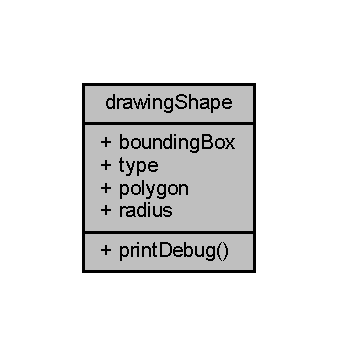
\includegraphics[width=162pt]{structdrawing_shape__coll__graph}
\end{center}
\end{figure}
\subsection*{Public Member Functions}
\begin{DoxyCompactItemize}
\item 
\mbox{\Hypertarget{structdrawing_shape_ad8778d93fedbd79a2ae09fa26bf73a63}\label{structdrawing_shape_ad8778d93fedbd79a2ae09fa26bf73a63}} 
void {\bfseries print\+Debug} ()
\end{DoxyCompactItemize}
\subsection*{Public Attributes}
\begin{DoxyCompactItemize}
\item 
\mbox{\Hypertarget{structdrawing_shape_a74c409162ad339b0475ece5f15d6f043}\label{structdrawing_shape_a74c409162ad339b0475ece5f15d6f043}} 
Q\+Rect {\bfseries bounding\+Box}
\item 
\mbox{\Hypertarget{structdrawing_shape_af3c271d20fd62c4e619d1ff7390b63e8}\label{structdrawing_shape_af3c271d20fd62c4e619d1ff7390b63e8}} 
drawing\+Mode\+::drawing\+Mode {\bfseries type}
\item 
\mbox{\Hypertarget{structdrawing_shape_a3aae768e541c892d7b03e935ecd0b2b9}\label{structdrawing_shape_a3aae768e541c892d7b03e935ecd0b2b9}} 
Q\+Polygon {\bfseries polygon}
\item 
\mbox{\Hypertarget{structdrawing_shape_a0dba9c87b530e092a592eeaa49afc21d}\label{structdrawing_shape_a0dba9c87b530e092a592eeaa49afc21d}} 
int {\bfseries radius}
\end{DoxyCompactItemize}


\subsection{Detailed Description}
structure to represent shape being drawn 

Definition at line 218 of file globals.\+h.



The documentation for this struct was generated from the following file\+:\begin{DoxyCompactItemize}
\item 
H\+:/\+Code\+Projects/\+Q\+T\+Projects/\+Targeter-\/msvc/globals.\+h\end{DoxyCompactItemize}

\hypertarget{structentropy_cluster}{}\section{entropy\+Cluster Struct Reference}
\label{structentropy_cluster}\index{entropy\+Cluster@{entropy\+Cluster}}


Collaboration diagram for entropy\+Cluster\+:
\nopagebreak
\begin{figure}[H]
\begin{center}
\leavevmode
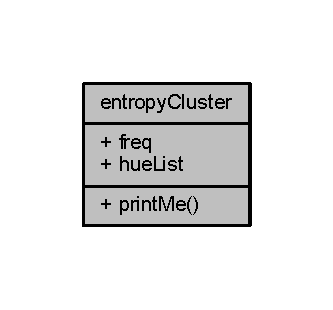
\includegraphics[width=160pt]{structentropy_cluster__coll__graph}
\end{center}
\end{figure}
\subsection*{Public Member Functions}
\begin{DoxyCompactItemize}
\item 
\mbox{\Hypertarget{structentropy_cluster_ac7bd664b978fbd56bea06eeadea3811c}\label{structentropy_cluster_ac7bd664b978fbd56bea06eeadea3811c}} 
void {\bfseries print\+Me} (std\+::string s=\char`\"{}\char`\"{})
\end{DoxyCompactItemize}
\subsection*{Public Attributes}
\begin{DoxyCompactItemize}
\item 
\mbox{\Hypertarget{structentropy_cluster_a3c49f6a3e21a396c409973ddf5a6c93e}\label{structentropy_cluster_a3c49f6a3e21a396c409973ddf5a6c93e}} 
float {\bfseries freq}
\item 
\mbox{\Hypertarget{structentropy_cluster_a3883cd312666c9aa28dfdd57f7bb5496}\label{structentropy_cluster_a3883cd312666c9aa28dfdd57f7bb5496}} 
std\+::vector$<$ int $>$ {\bfseries hue\+List}
\end{DoxyCompactItemize}


\subsection{Detailed Description}


Definition at line 199 of file globals.\+h.



The documentation for this struct was generated from the following file\+:\begin{DoxyCompactItemize}
\item 
H\+:/\+Code\+Projects/\+Q\+T\+Projects/\+Targeter-\/msvc/globals.\+h\end{DoxyCompactItemize}

\hypertarget{class_focus_stack}{}\section{Focus\+Stack Class Reference}
\label{class_focus_stack}\index{Focus\+Stack@{Focus\+Stack}}


{\ttfamily \#include $<$Focus\+Stack.\+h$>$}



Collaboration diagram for Focus\+Stack\+:
\nopagebreak
\begin{figure}[H]
\begin{center}
\leavevmode
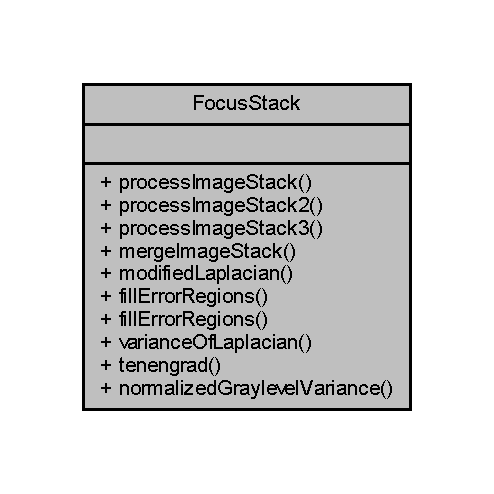
\includegraphics[width=237pt]{class_focus_stack__coll__graph}
\end{center}
\end{figure}
\subsection*{Static Public Member Functions}
\begin{DoxyCompactItemize}
\item 
static cv\+::\+Mat $\ast$ \hyperlink{class_focus_stack_aca40f92aa05f5aa0a2e58c846bb69a75}{process\+Image\+Stack} (std\+::vector$<$ \hyperlink{classtargeter_image}{targeter\+Image} $>$ \&image\+Stack, std\+::vector$<$ int $>$ \&image\+Indexes, \hyperlink{class_main_window}{Main\+Window} $\ast$p\+Main\+Window)
\item 
static cv\+::\+Mat $\ast$ \hyperlink{class_focus_stack_a6342aff10617c4346b32f61ea549b378}{process\+Image\+Stack2} (std\+::vector$<$ \hyperlink{classtargeter_image}{targeter\+Image} $>$ \&image\+Stack, std\+::vector$<$ int $>$ \&image\+Indexes, \hyperlink{class_main_window}{Main\+Window} $\ast$p\+Main\+Window)
\item 
static cv\+::\+Mat $\ast$ \hyperlink{class_focus_stack_a141b4869671825fed21068a9c9f2c150}{process\+Image\+Stack3} (std\+::vector$<$ \hyperlink{classtargeter_image}{targeter\+Image} $>$ \&image\+Stack, std\+::vector$<$ int $>$ \&image\+Indexes, \hyperlink{class_main_window}{Main\+Window} $\ast$p\+Main\+Window)
\item 
static cv\+::\+Mat $\ast$ \hyperlink{class_focus_stack_ac55d6cde57441ffd9b023fc936529802}{merge\+Image\+Stack} (std\+::vector$<$ \hyperlink{classtargeter_image}{targeter\+Image} $>$ \&image\+Stack, cv\+::\+Mat index\+Image, int w, int h)
\item 
static double \hyperlink{class_focus_stack_a4aaf824aa1df503f99c24e3cf9a40189}{modified\+Laplacian} (const cv\+::\+Mat \&src)
\item 
static void \hyperlink{class_focus_stack_a1ab8c45eab892975ad3dbdf039add315}{fill\+Error\+Regions} (int $\ast$im, int w, int h, int f\+Size, int No\+Focus\+Images)
\item 
\mbox{\Hypertarget{class_focus_stack_ae47c1a7f8114be3d4b75949516e49002}\label{class_focus_stack_ae47c1a7f8114be3d4b75949516e49002}} 
static void {\bfseries fill\+Error\+Regions} (cv\+::\+Mat \&im, int w, int h, int f\+Size, int No\+Focus\+Images)
\item 
static double \hyperlink{class_focus_stack_afc9e634d57f2b2f0df1d6d615cd44c15}{variance\+Of\+Laplacian} (const cv\+::\+Mat \&src)
\item 
static double \hyperlink{class_focus_stack_a6b65715e671ef5a016d9e216705d687d}{tenengrad} (const cv\+::\+Mat \&src, int ksize)
\item 
static double \hyperlink{class_focus_stack_ad1ceb7d7b721e11b2861332823c0b09d}{normalized\+Graylevel\+Variance} (const cv\+::\+Mat \&src)
\end{DoxyCompactItemize}


\subsection{Detailed Description}
class that manages performing focus stack, ie. takes image sequence and combines them into single in focus image 

Definition at line 12 of file Focus\+Stack.\+h.



\subsection{Member Function Documentation}
\mbox{\Hypertarget{class_focus_stack_a1ab8c45eab892975ad3dbdf039add315}\label{class_focus_stack_a1ab8c45eab892975ad3dbdf039add315}} 
\index{Focus\+Stack@{Focus\+Stack}!fill\+Error\+Regions@{fill\+Error\+Regions}}
\index{fill\+Error\+Regions@{fill\+Error\+Regions}!Focus\+Stack@{Focus\+Stack}}
\subsubsection{\texorpdfstring{fill\+Error\+Regions()}{fillErrorRegions()}}
{\footnotesize\ttfamily void Focus\+Stack\+::fill\+Error\+Regions (\begin{DoxyParamCaption}\item[{int $\ast$}]{im,  }\item[{int}]{w,  }\item[{int}]{h,  }\item[{int}]{f\+Size,  }\item[{int}]{No\+Focus\+Images }\end{DoxyParamCaption})\hspace{0.3cm}{\ttfamily [static]}}

Compares neighbouring pixels to determine best value for focusing

\begin{DoxyAuthor}{Author}
David Watts 
\end{DoxyAuthor}
\begin{DoxySince}{Since}
2017/03/07
\end{DoxySince}
Full\+Name \hyperlink{class_focus_stack_a1ab8c45eab892975ad3dbdf039add315}{Focus\+Stack\+::fill\+Error\+Regions} Qualifier 
\begin{DoxyParams}{Parameters}
{\em int} & $\ast$ im \\
\hline
{\em int} & w \\
\hline
{\em int} & h \\
\hline
{\em int} & f\+Size \\
\hline
{\em int} & No\+Focus\+Images \\
\hline
\end{DoxyParams}
\begin{DoxyReturn}{Returns}
void Access public 
\end{DoxyReturn}


Definition at line 456 of file Focus\+Stack.\+cpp.

Here is the caller graph for this function\+:
\nopagebreak
\begin{figure}[H]
\begin{center}
\leavevmode
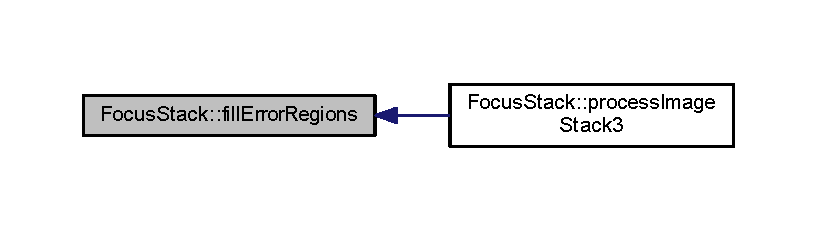
\includegraphics[width=350pt]{class_focus_stack_a1ab8c45eab892975ad3dbdf039add315_icgraph}
\end{center}
\end{figure}
\mbox{\Hypertarget{class_focus_stack_ac55d6cde57441ffd9b023fc936529802}\label{class_focus_stack_ac55d6cde57441ffd9b023fc936529802}} 
\index{Focus\+Stack@{Focus\+Stack}!merge\+Image\+Stack@{merge\+Image\+Stack}}
\index{merge\+Image\+Stack@{merge\+Image\+Stack}!Focus\+Stack@{Focus\+Stack}}
\subsubsection{\texorpdfstring{merge\+Image\+Stack()}{mergeImageStack()}}
{\footnotesize\ttfamily Mat $\ast$ Focus\+Stack\+::merge\+Image\+Stack (\begin{DoxyParamCaption}\item[{std\+::vector$<$ \hyperlink{classtargeter_image}{targeter\+Image} $>$ \&}]{image\+Stack,  }\item[{cv\+::\+Mat}]{index\+Image,  }\item[{int}]{w,  }\item[{int}]{h }\end{DoxyParamCaption})\hspace{0.3cm}{\ttfamily [static]}}

Merges images based on indexing the vector using the values in index\+Image

\begin{DoxyAuthor}{Author}
David Watts 
\end{DoxyAuthor}
\begin{DoxySince}{Since}
2017/03/07
\end{DoxySince}
Full\+Name \hyperlink{class_focus_stack_ac55d6cde57441ffd9b023fc936529802}{Focus\+Stack\+::merge\+Image\+Stack} Qualifier 
\begin{DoxyParams}{Parameters}
{\em Q\+Vector$<$targeter\+Image$>$} & \& image\+Stack \\
\hline
{\em Mat} & index\+Image \\
\hline
{\em int} & w \\
\hline
{\em int} & h \\
\hline
\end{DoxyParams}
\begin{DoxyReturn}{Returns}
cv\+::\+Mat$\ast$ Access public 
\end{DoxyReturn}


Definition at line 408 of file Focus\+Stack.\+cpp.

Here is the caller graph for this function\+:
\nopagebreak
\begin{figure}[H]
\begin{center}
\leavevmode
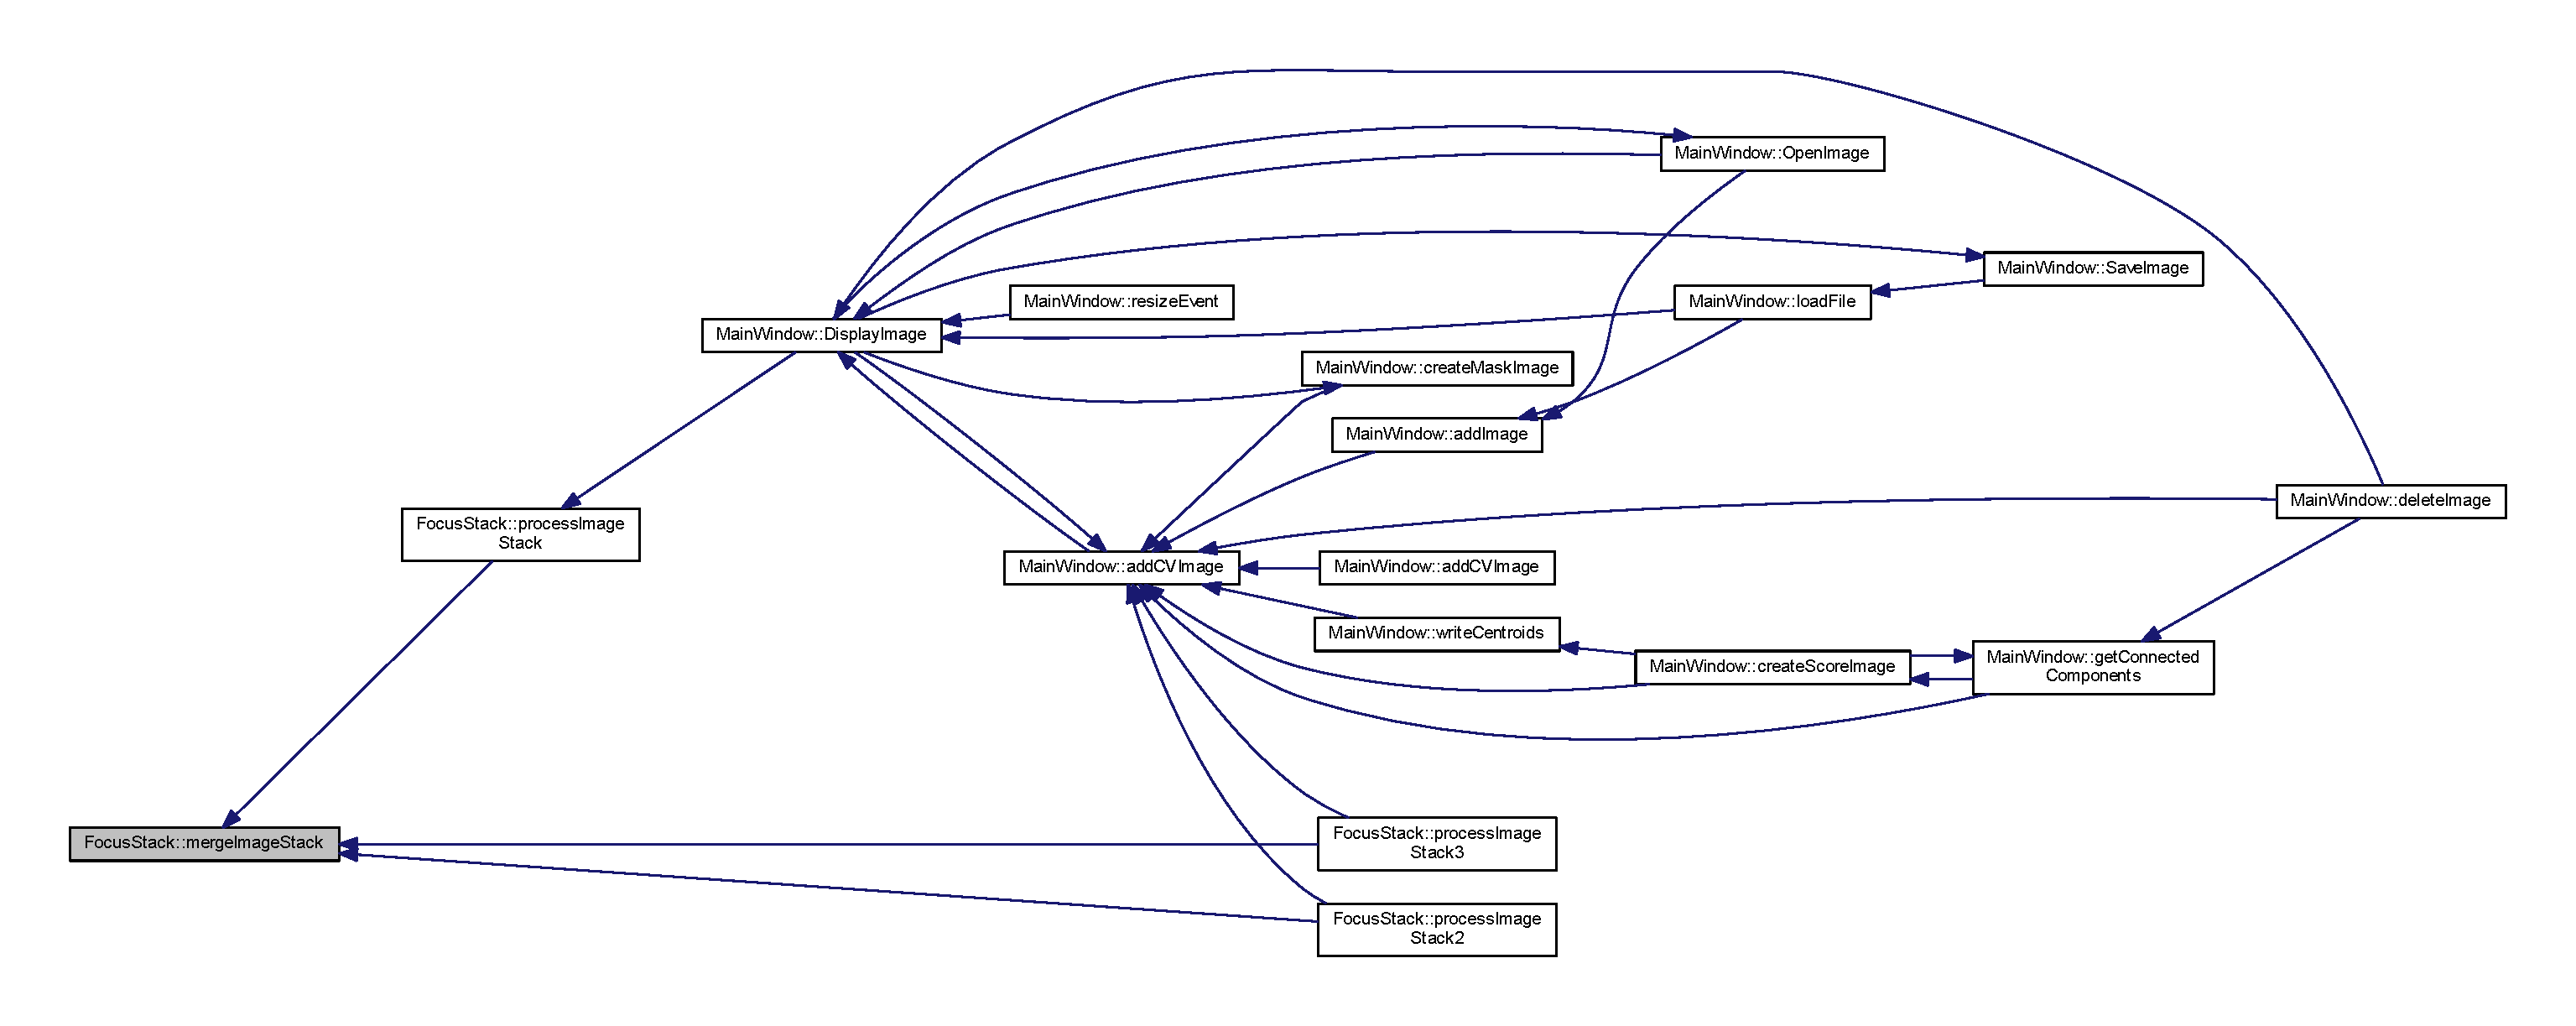
\includegraphics[width=350pt]{class_focus_stack_ac55d6cde57441ffd9b023fc936529802_icgraph}
\end{center}
\end{figure}
\mbox{\Hypertarget{class_focus_stack_a4aaf824aa1df503f99c24e3cf9a40189}\label{class_focus_stack_a4aaf824aa1df503f99c24e3cf9a40189}} 
\index{Focus\+Stack@{Focus\+Stack}!modified\+Laplacian@{modified\+Laplacian}}
\index{modified\+Laplacian@{modified\+Laplacian}!Focus\+Stack@{Focus\+Stack}}
\subsubsection{\texorpdfstring{modified\+Laplacian()}{modifiedLaplacian()}}
{\footnotesize\ttfamily double Focus\+Stack\+::modified\+Laplacian (\begin{DoxyParamCaption}\item[{const cv\+::\+Mat \&}]{src }\end{DoxyParamCaption})\hspace{0.3cm}{\ttfamily [static]}}

Open\+CV port of \textquotesingle{}L\+A\+PM\textquotesingle{} algorithm (Nayar89)

\begin{DoxyAuthor}{Author}
David Watts 
\end{DoxyAuthor}
\begin{DoxySince}{Since}
2017/03/07
\end{DoxySince}
Full\+Name \hyperlink{class_focus_stack_a4aaf824aa1df503f99c24e3cf9a40189}{Focus\+Stack\+::modified\+Laplacian} Qualifier 
\begin{DoxyParams}{Parameters}
{\em const} & cv\+::\+Mat \& src \\
\hline
\end{DoxyParams}
\begin{DoxyReturn}{Returns}
double Access public 
\end{DoxyReturn}


Definition at line 610 of file Focus\+Stack.\+cpp.

\mbox{\Hypertarget{class_focus_stack_ad1ceb7d7b721e11b2861332823c0b09d}\label{class_focus_stack_ad1ceb7d7b721e11b2861332823c0b09d}} 
\index{Focus\+Stack@{Focus\+Stack}!normalized\+Graylevel\+Variance@{normalized\+Graylevel\+Variance}}
\index{normalized\+Graylevel\+Variance@{normalized\+Graylevel\+Variance}!Focus\+Stack@{Focus\+Stack}}
\subsubsection{\texorpdfstring{normalized\+Graylevel\+Variance()}{normalizedGraylevelVariance()}}
{\footnotesize\ttfamily double Focus\+Stack\+::normalized\+Graylevel\+Variance (\begin{DoxyParamCaption}\item[{const cv\+::\+Mat \&}]{src }\end{DoxyParamCaption})\hspace{0.3cm}{\ttfamily [static]}}

Open\+CV port of \textquotesingle{}G\+L\+VN\textquotesingle{} algorithm (Santos97)

\begin{DoxyAuthor}{Author}
David Watts 
\end{DoxyAuthor}
\begin{DoxySince}{Since}
2017/03/07
\end{DoxySince}
Full\+Name \hyperlink{class_focus_stack_ad1ceb7d7b721e11b2861332823c0b09d}{Focus\+Stack\+::normalized\+Graylevel\+Variance} Qualifier 
\begin{DoxyParams}{Parameters}
{\em const} & cv\+::\+Mat \& src \\
\hline
\end{DoxyParams}
\begin{DoxyReturn}{Returns}
double Access public 
\end{DoxyReturn}


Definition at line 698 of file Focus\+Stack.\+cpp.

\mbox{\Hypertarget{class_focus_stack_aca40f92aa05f5aa0a2e58c846bb69a75}\label{class_focus_stack_aca40f92aa05f5aa0a2e58c846bb69a75}} 
\index{Focus\+Stack@{Focus\+Stack}!process\+Image\+Stack@{process\+Image\+Stack}}
\index{process\+Image\+Stack@{process\+Image\+Stack}!Focus\+Stack@{Focus\+Stack}}
\subsubsection{\texorpdfstring{process\+Image\+Stack()}{processImageStack()}}
{\footnotesize\ttfamily Mat $\ast$ Focus\+Stack\+::process\+Image\+Stack (\begin{DoxyParamCaption}\item[{std\+::vector$<$ \hyperlink{classtargeter_image}{targeter\+Image} $>$ \&}]{image\+Stack,  }\item[{std\+::vector$<$ int $>$ \&}]{image\+Indexes,  }\item[{\hyperlink{class_main_window}{Main\+Window} $\ast$}]{p\+Main\+Window }\end{DoxyParamCaption})\hspace{0.3cm}{\ttfamily [static]}}

Creates a single \textquotesingle{}in focus\textquotesingle{} image from a vector of images partially in focus (focus stack)

\begin{DoxyAuthor}{Author}
David Watts 
\end{DoxyAuthor}
\begin{DoxySince}{Since}
2017/03/07
\end{DoxySince}
Full\+Name \hyperlink{class_focus_stack_aca40f92aa05f5aa0a2e58c846bb69a75}{Focus\+Stack\+::process\+Image\+Stack} Qualifier 
\begin{DoxyParams}{Parameters}
{\em Q\+Vector$<$targeter\+Image$>$} & \& image\+Stack \\
\hline
{\em Q\+Vector$<$int$>$} & \& image\+Indexes \\
\hline
{\em \hyperlink{class_main_window}{Main\+Window}} & $\ast$ p\+Main\+Window \\
\hline
\end{DoxyParams}
\begin{DoxyReturn}{Returns}
cv\+::\+Mat$\ast$ Access public 
\end{DoxyReturn}


Definition at line 35 of file Focus\+Stack.\+cpp.

Here is the call graph for this function\+:
\nopagebreak
\begin{figure}[H]
\begin{center}
\leavevmode
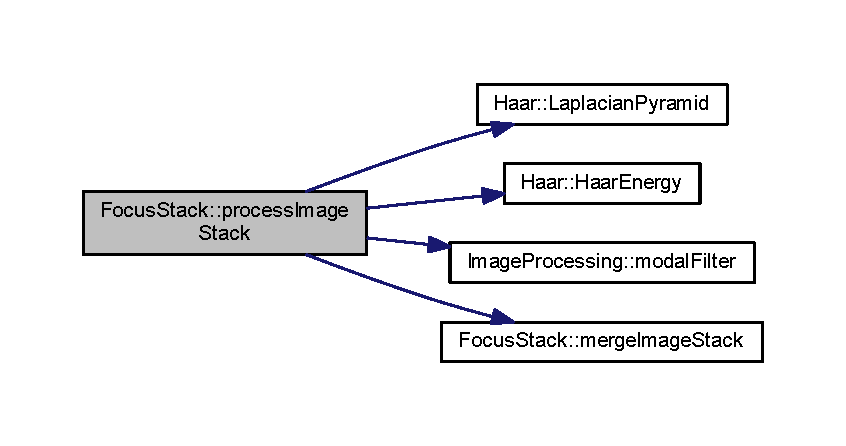
\includegraphics[width=350pt]{class_focus_stack_aca40f92aa05f5aa0a2e58c846bb69a75_cgraph}
\end{center}
\end{figure}
Here is the caller graph for this function\+:
\nopagebreak
\begin{figure}[H]
\begin{center}
\leavevmode
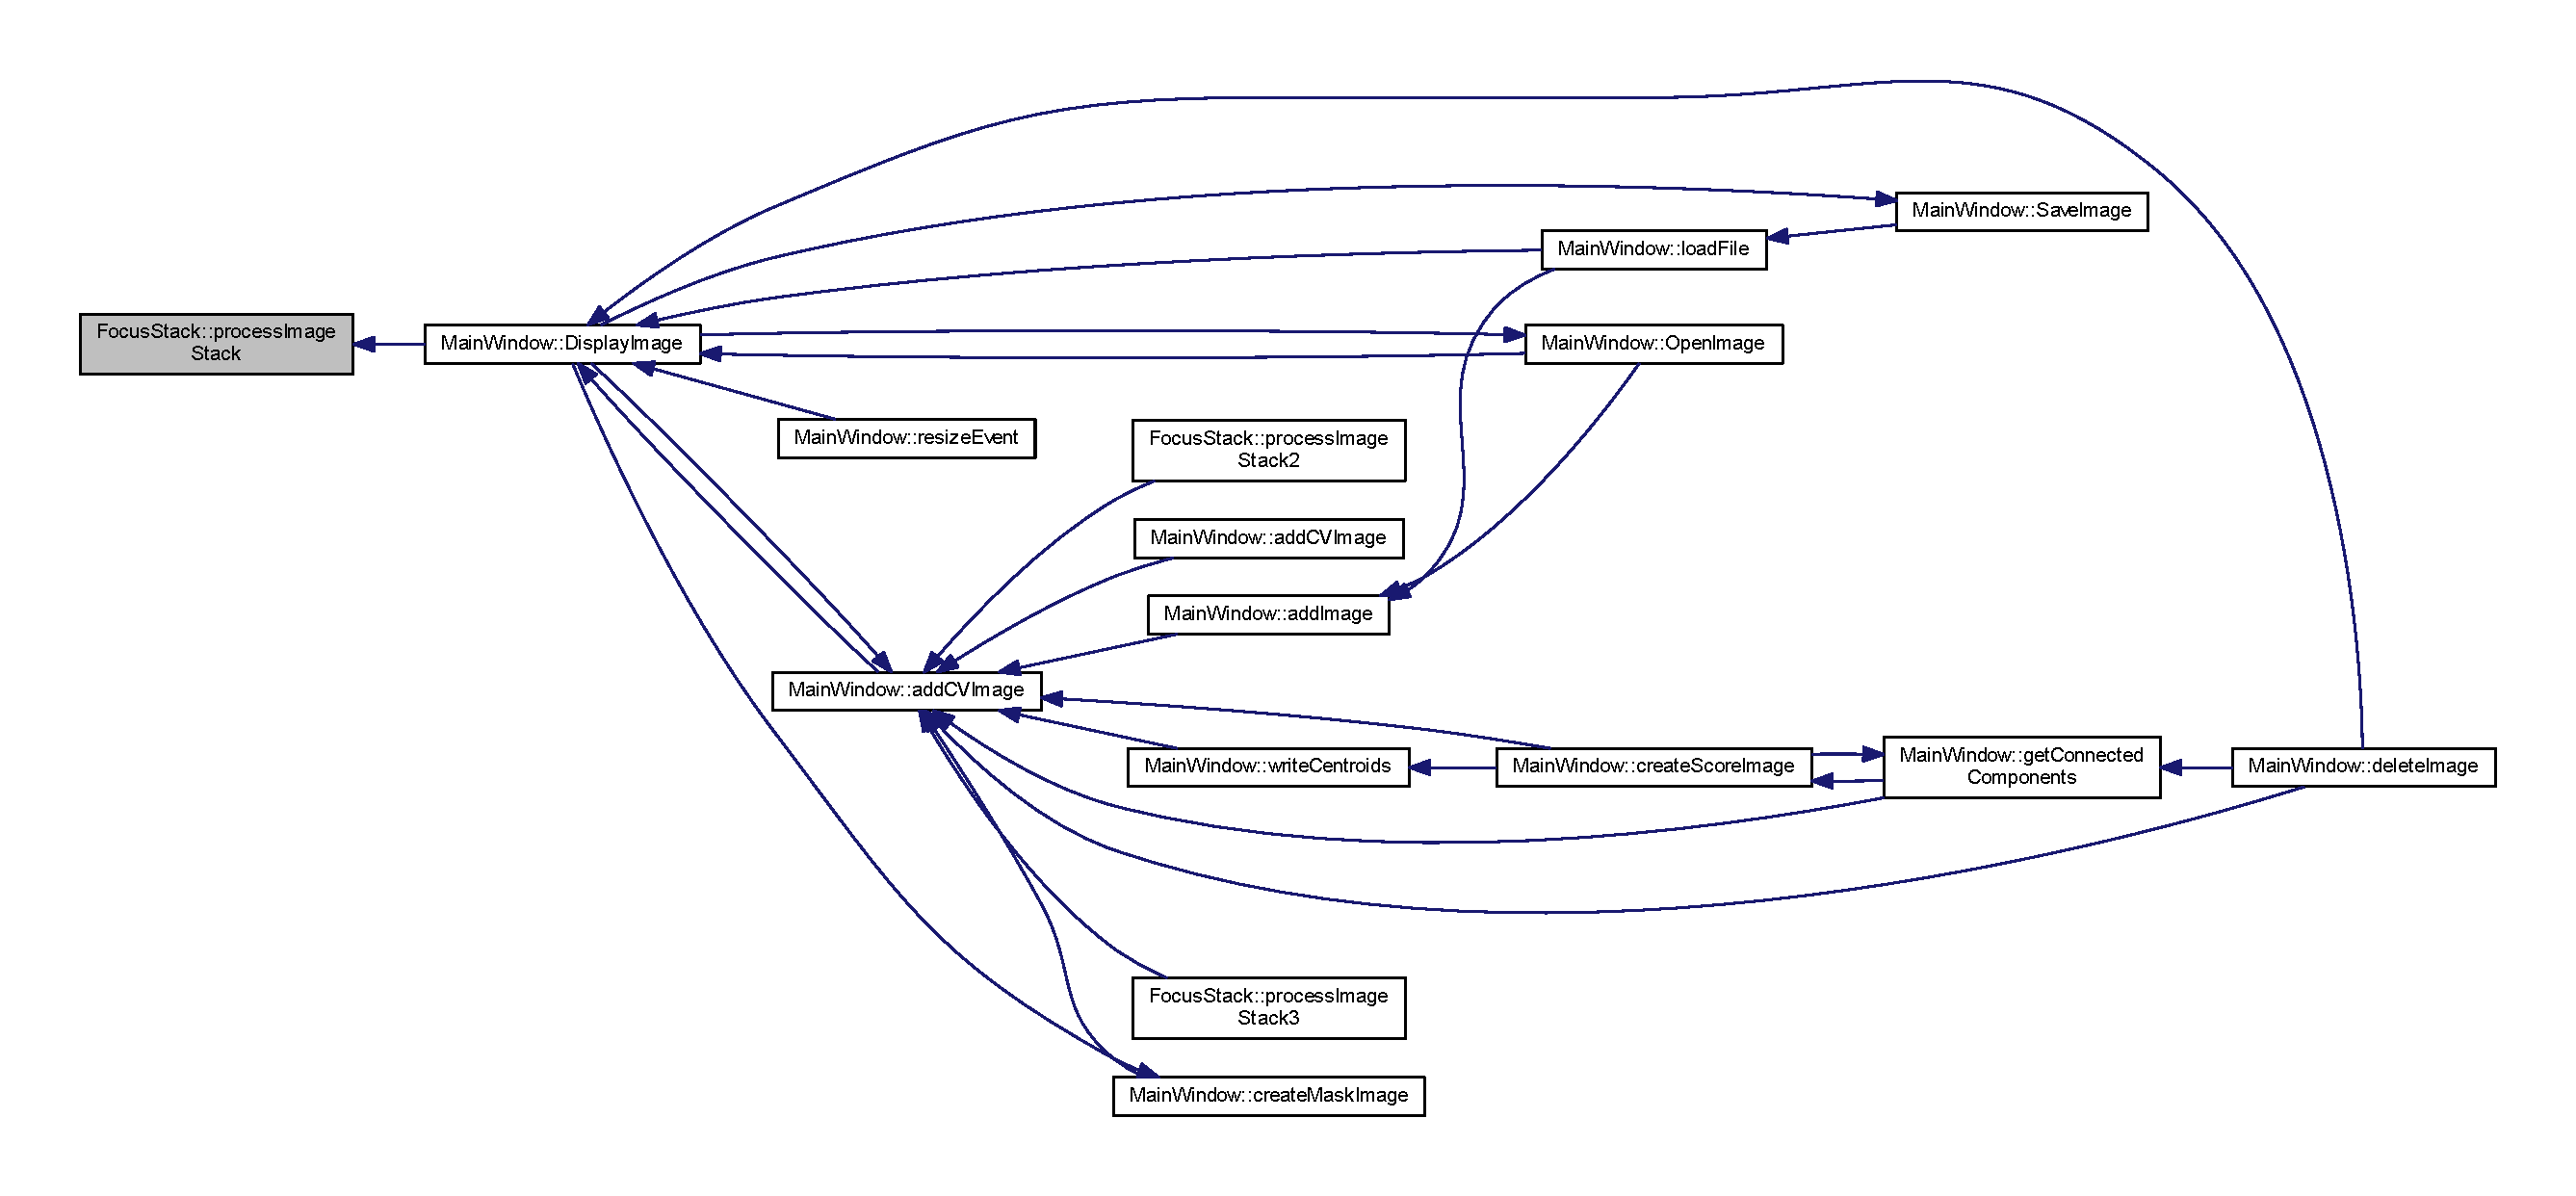
\includegraphics[width=350pt]{class_focus_stack_aca40f92aa05f5aa0a2e58c846bb69a75_icgraph}
\end{center}
\end{figure}
\mbox{\Hypertarget{class_focus_stack_a6342aff10617c4346b32f61ea549b378}\label{class_focus_stack_a6342aff10617c4346b32f61ea549b378}} 
\index{Focus\+Stack@{Focus\+Stack}!process\+Image\+Stack2@{process\+Image\+Stack2}}
\index{process\+Image\+Stack2@{process\+Image\+Stack2}!Focus\+Stack@{Focus\+Stack}}
\subsubsection{\texorpdfstring{process\+Image\+Stack2()}{processImageStack2()}}
{\footnotesize\ttfamily cv\+::\+Mat $\ast$ Focus\+Stack\+::process\+Image\+Stack2 (\begin{DoxyParamCaption}\item[{std\+::vector$<$ \hyperlink{classtargeter_image}{targeter\+Image} $>$ \&}]{image\+Stack,  }\item[{std\+::vector$<$ int $>$ \&}]{image\+Indexes,  }\item[{\hyperlink{class_main_window}{Main\+Window} $\ast$}]{p\+Main\+Window }\end{DoxyParamCaption})\hspace{0.3cm}{\ttfamily [static]}}

Creates a single \textquotesingle{}in focus\textquotesingle{} image from a vector of images partially in focus (focus stack) (alternative implementation)

\begin{DoxyAuthor}{Author}
David Watts 
\end{DoxyAuthor}
\begin{DoxySince}{Since}
2017/03/07
\end{DoxySince}
Full\+Name \hyperlink{class_focus_stack_a6342aff10617c4346b32f61ea549b378}{Focus\+Stack\+::process\+Image\+Stack2} Qualifier 
\begin{DoxyParams}{Parameters}
{\em Q\+Vector$<$targeter\+Image$>$} & \& image\+Stack \\
\hline
{\em Q\+Vector$<$int$>$} & \& image\+Indexes \\
\hline
{\em \hyperlink{class_main_window}{Main\+Window}} & $\ast$ p\+Main\+Window \\
\hline
\end{DoxyParams}
\begin{DoxyReturn}{Returns}
cv\+::\+Mat$\ast$ Access public 
\end{DoxyReturn}


Definition at line 290 of file Focus\+Stack.\+cpp.

Here is the call graph for this function\+:
\nopagebreak
\begin{figure}[H]
\begin{center}
\leavevmode
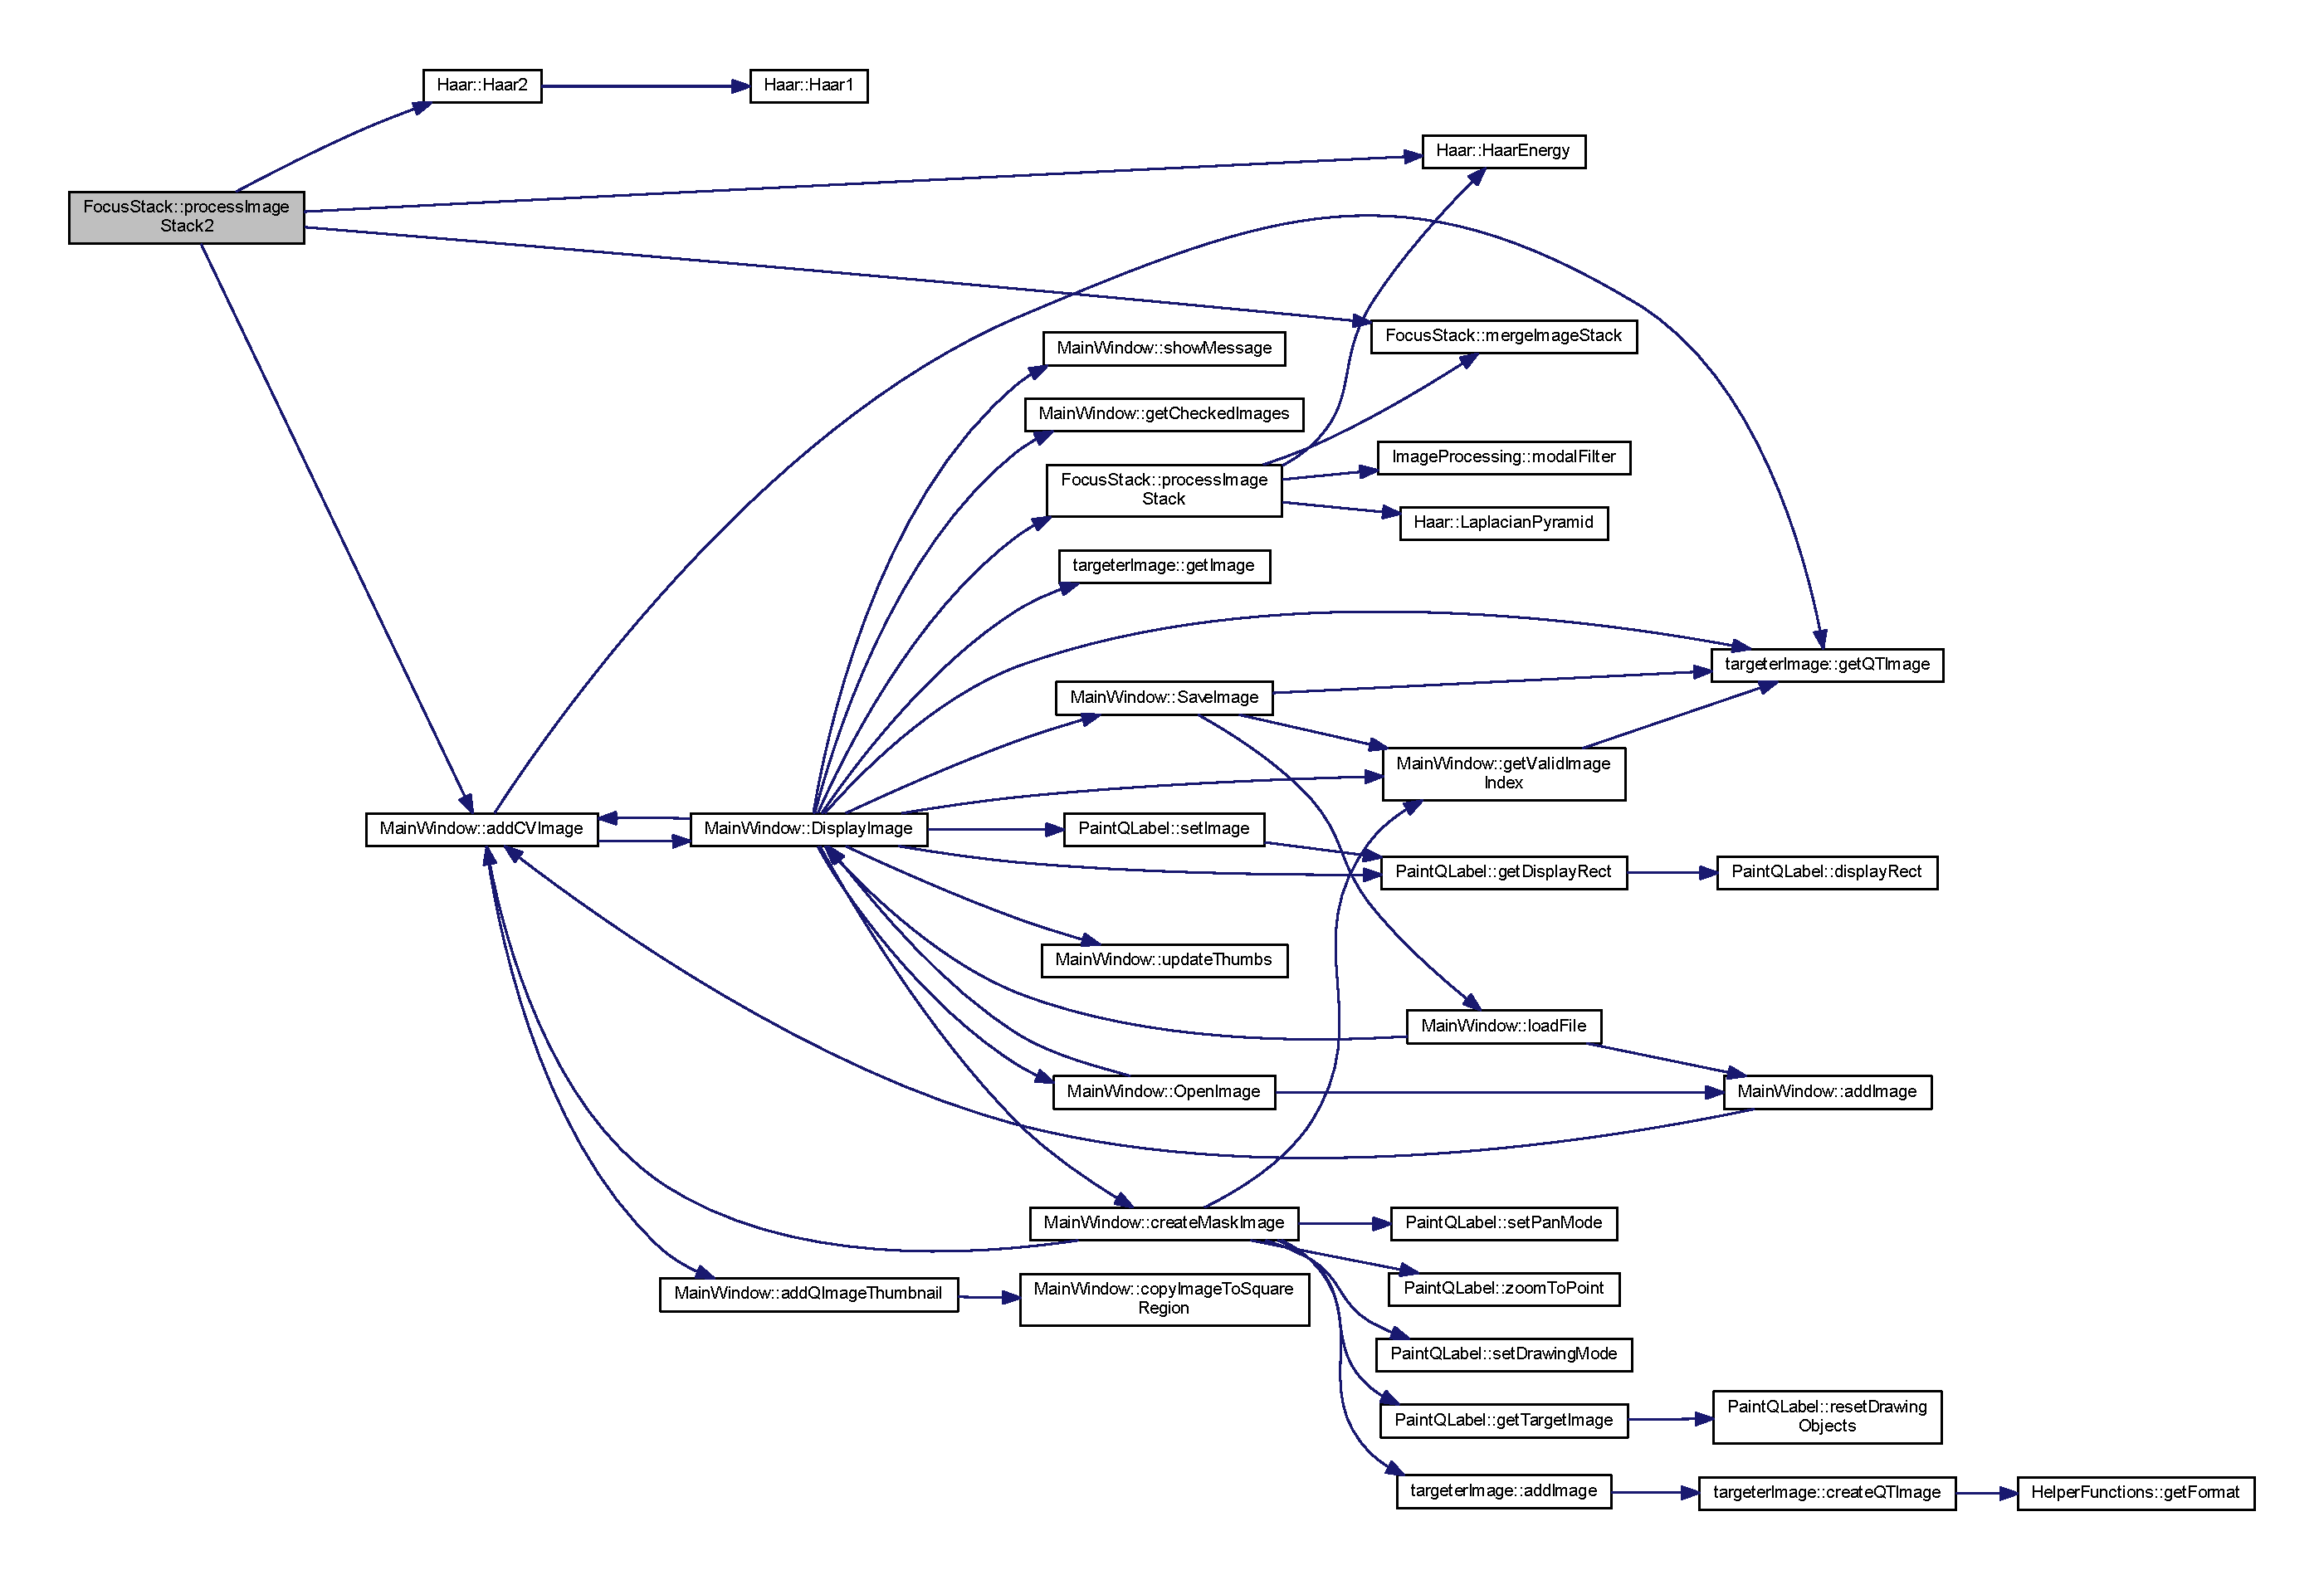
\includegraphics[width=350pt]{class_focus_stack_a6342aff10617c4346b32f61ea549b378_cgraph}
\end{center}
\end{figure}
\mbox{\Hypertarget{class_focus_stack_a141b4869671825fed21068a9c9f2c150}\label{class_focus_stack_a141b4869671825fed21068a9c9f2c150}} 
\index{Focus\+Stack@{Focus\+Stack}!process\+Image\+Stack3@{process\+Image\+Stack3}}
\index{process\+Image\+Stack3@{process\+Image\+Stack3}!Focus\+Stack@{Focus\+Stack}}
\subsubsection{\texorpdfstring{process\+Image\+Stack3()}{processImageStack3()}}
{\footnotesize\ttfamily cv\+::\+Mat $\ast$ Focus\+Stack\+::process\+Image\+Stack3 (\begin{DoxyParamCaption}\item[{std\+::vector$<$ \hyperlink{classtargeter_image}{targeter\+Image} $>$ \&}]{image\+Stack,  }\item[{std\+::vector$<$ int $>$ \&}]{image\+Indexes,  }\item[{\hyperlink{class_main_window}{Main\+Window} $\ast$}]{p\+Main\+Window }\end{DoxyParamCaption})\hspace{0.3cm}{\ttfamily [static]}}

Creates a single \textquotesingle{}in focus\textquotesingle{} image from a vector of images partially in focus (focus stack) (alternative implementation)

\begin{DoxyAuthor}{Author}
David Watts 
\end{DoxyAuthor}
\begin{DoxySince}{Since}
2017/03/07
\end{DoxySince}
Full\+Name \hyperlink{class_focus_stack_a141b4869671825fed21068a9c9f2c150}{Focus\+Stack\+::process\+Image\+Stack3} Qualifier 
\begin{DoxyParams}{Parameters}
{\em Q\+Vector$<$targeter\+Image$>$} & \& image\+Stack \\
\hline
{\em Q\+Vector$<$int$>$} & \& image\+Indexes \\
\hline
{\em \hyperlink{class_main_window}{Main\+Window}} & $\ast$ p\+Main\+Window \\
\hline
\end{DoxyParams}
\begin{DoxyReturn}{Returns}
cv\+::\+Mat$\ast$ Access public 
\end{DoxyReturn}


Definition at line 164 of file Focus\+Stack.\+cpp.

Here is the call graph for this function\+:
\nopagebreak
\begin{figure}[H]
\begin{center}
\leavevmode
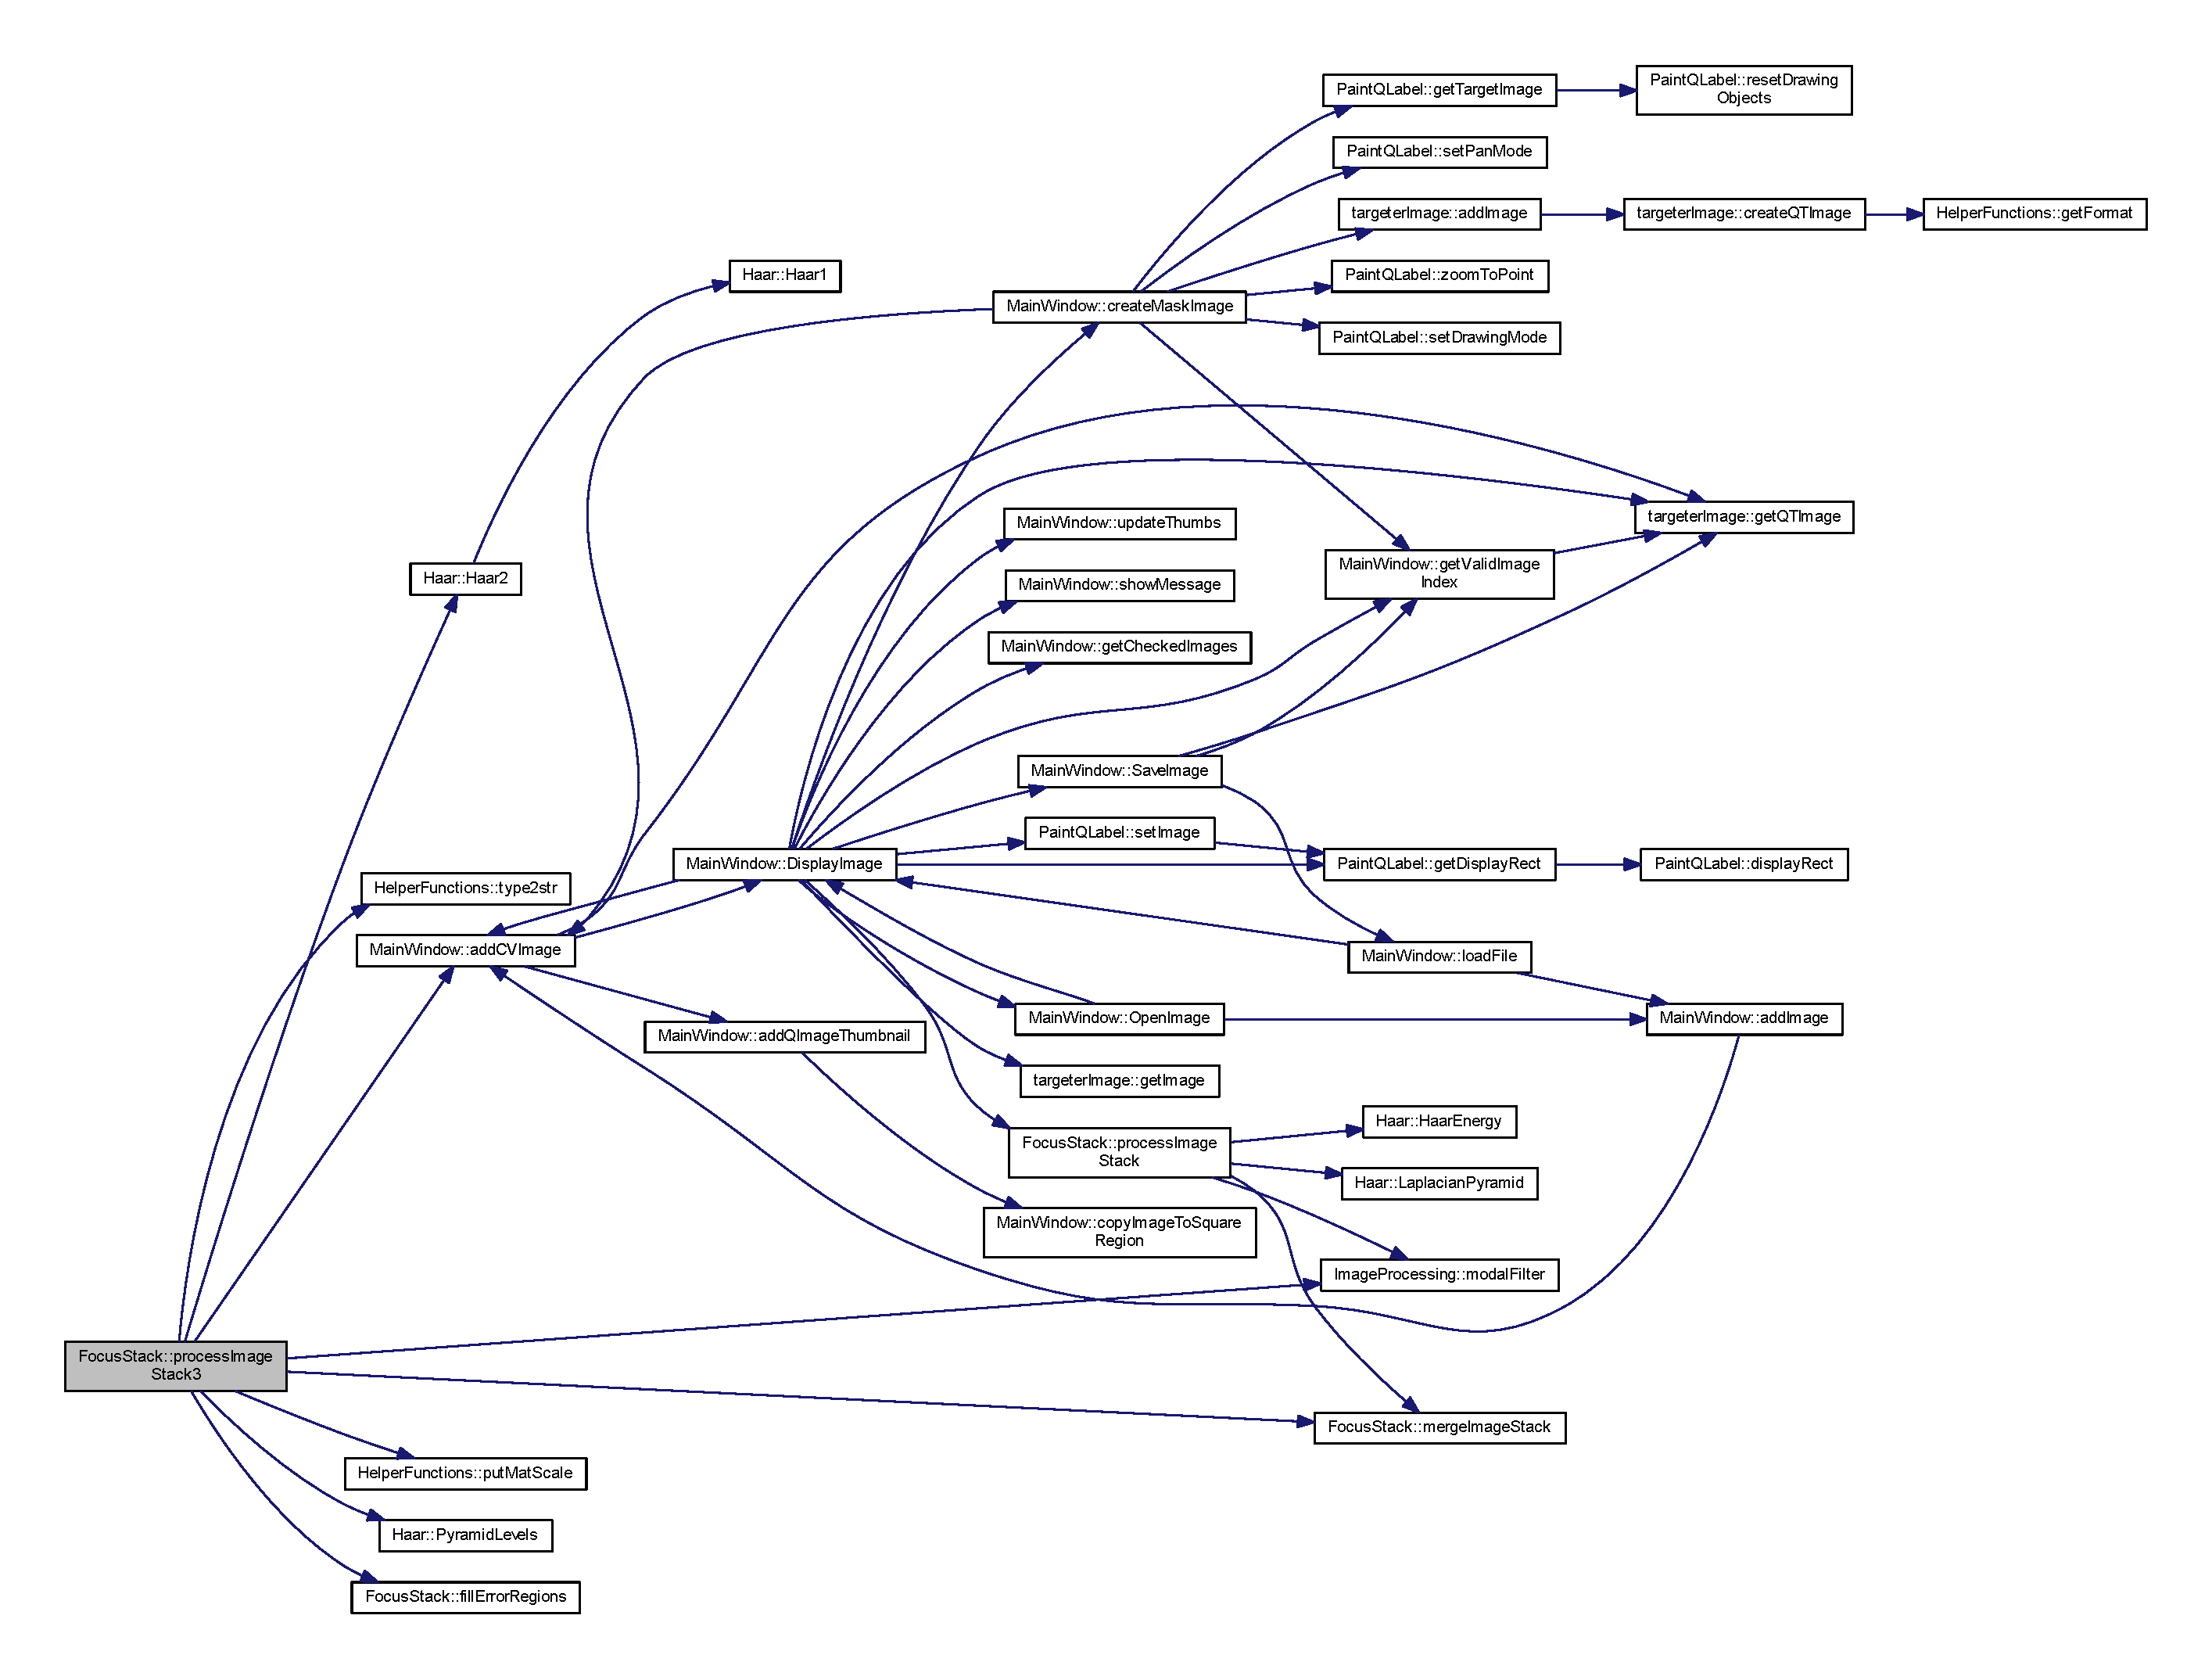
\includegraphics[width=350pt]{class_focus_stack_a141b4869671825fed21068a9c9f2c150_cgraph}
\end{center}
\end{figure}
\mbox{\Hypertarget{class_focus_stack_a6b65715e671ef5a016d9e216705d687d}\label{class_focus_stack_a6b65715e671ef5a016d9e216705d687d}} 
\index{Focus\+Stack@{Focus\+Stack}!tenengrad@{tenengrad}}
\index{tenengrad@{tenengrad}!Focus\+Stack@{Focus\+Stack}}
\subsubsection{\texorpdfstring{tenengrad()}{tenengrad()}}
{\footnotesize\ttfamily double Focus\+Stack\+::tenengrad (\begin{DoxyParamCaption}\item[{const cv\+::\+Mat \&}]{src,  }\item[{int}]{ksize }\end{DoxyParamCaption})\hspace{0.3cm}{\ttfamily [static]}}

Open\+CV port of \textquotesingle{}T\+E\+NG\textquotesingle{} algorithm (Krotkov86)

\begin{DoxyAuthor}{Author}
David Watts 
\end{DoxyAuthor}
\begin{DoxySince}{Since}
2017/03/07
\end{DoxySince}
Full\+Name \hyperlink{class_focus_stack_a6b65715e671ef5a016d9e216705d687d}{Focus\+Stack\+::tenengrad} Qualifier 
\begin{DoxyParams}{Parameters}
{\em const} & cv\+::\+Mat \& src \\
\hline
{\em int} & ksize \\
\hline
\end{DoxyParams}
\begin{DoxyReturn}{Returns}
double Access public 
\end{DoxyReturn}


Definition at line 671 of file Focus\+Stack.\+cpp.

\mbox{\Hypertarget{class_focus_stack_afc9e634d57f2b2f0df1d6d615cd44c15}\label{class_focus_stack_afc9e634d57f2b2f0df1d6d615cd44c15}} 
\index{Focus\+Stack@{Focus\+Stack}!variance\+Of\+Laplacian@{variance\+Of\+Laplacian}}
\index{variance\+Of\+Laplacian@{variance\+Of\+Laplacian}!Focus\+Stack@{Focus\+Stack}}
\subsubsection{\texorpdfstring{variance\+Of\+Laplacian()}{varianceOfLaplacian()}}
{\footnotesize\ttfamily double Focus\+Stack\+::variance\+Of\+Laplacian (\begin{DoxyParamCaption}\item[{const cv\+::\+Mat \&}]{src }\end{DoxyParamCaption})\hspace{0.3cm}{\ttfamily [static]}}

Open\+CV port of \textquotesingle{}L\+A\+PV\textquotesingle{} algorithm (Pech2000)

\begin{DoxyAuthor}{Author}
David Watts 
\end{DoxyAuthor}
\begin{DoxySince}{Since}
2017/03/07
\end{DoxySince}
Full\+Name \hyperlink{class_focus_stack_afc9e634d57f2b2f0df1d6d615cd44c15}{Focus\+Stack\+::variance\+Of\+Laplacian} Qualifier 
\begin{DoxyParams}{Parameters}
{\em const} & cv\+::\+Mat \& src \\
\hline
\end{DoxyParams}
\begin{DoxyReturn}{Returns}
double Access public 
\end{DoxyReturn}


Definition at line 643 of file Focus\+Stack.\+cpp.



The documentation for this class was generated from the following files\+:\begin{DoxyCompactItemize}
\item 
H\+:/\+Code\+Projects/\+Q\+T\+Projects/\+Targeter-\/msvc/Focus\+Stack.\+h\item 
H\+:/\+Code\+Projects/\+Q\+T\+Projects/\+Targeter-\/msvc/Focus\+Stack.\+cpp\end{DoxyCompactItemize}

\hypertarget{class_haar}{}\section{Haar Class Reference}
\label{class_haar}\index{Haar@{Haar}}


Collaboration diagram for Haar\+:
\nopagebreak
\begin{figure}[H]
\begin{center}
\leavevmode
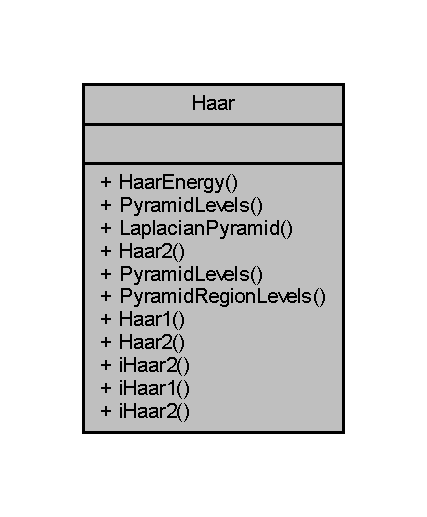
\includegraphics[width=205pt]{class_haar__coll__graph}
\end{center}
\end{figure}
\subsection*{Static Public Member Functions}
\begin{DoxyCompactItemize}
\item 
static void \hyperlink{class_haar_afa323789e73c94995eba32e09d9aa026}{Haar\+Energy} (cv\+::\+Mat data, cv\+::\+Mat \&energy\+Image, int width, int height, int iterations, bool laplace=false, bool b\+Square=true)
\item 
static cv\+::\+Mat \hyperlink{class_haar_a5a0726cb9e3a28295ba4ac64f654aa36}{Pyramid\+Levels} (cv\+::\+Mat data, int width, int height, int iterations, const int No\+Focus\+Images)
\item 
static cv\+::\+Mat \hyperlink{class_haar_ad85443bf4bbe9d65be10acbd0d89093b}{Laplacian\+Pyramid} (cv\+::\+Mat im, int levels, bool include\+Scale=true)
\item 
static void \hyperlink{class_haar_afde8fa7a1d65b505185a29fc7eaf4b2d}{Haar2} (cv\+::\+Mat \&data, int iterations)
\item 
{\footnotesize template$<$class T $>$ }\\static T $\ast$ \hyperlink{class_haar_a6724557f8d0a1660df2a9de85d7ce523}{Pyramid\+Levels} (T $\ast$data, int width, int height, int iterations, int No\+Focus\+Images)
\item 
{\footnotesize template$<$class T $>$ }\\static T $\ast$ \hyperlink{class_haar_a4f48761ec2f91c74df7ef6b501238d2a}{Pyramid\+Region\+Levels} (T $\ast$data, int width, int height, int iterations, int No\+Focus\+Images)
\item 
{\footnotesize template$<$class T $>$ }\\static void \hyperlink{class_haar_a44ab3d3043f2a9c2145629a242e6ed0f}{Haar1} (T $\ast$data, int n)
\item 
{\footnotesize template$<$class T $>$ }\\static void \hyperlink{class_haar_a4b2951fd5ec6f760fc94bd4273e2c544}{Haar2} (T $\ast$data, int width, int height, int iterations, bool Abs\+Image=false)
\item 
{\footnotesize template$<$class T $>$ }\\static void \hyperlink{class_haar_ab2c372ee9f5eec084066ba52de18fbbe}{i\+Haar2} (T $\ast$data, int width, int height, int iterations)
\item 
{\footnotesize template$<$class T $>$ }\\static void \hyperlink{class_haar_aedd7102138b5f942b7fbd539b1ff8143}{i\+Haar1} (T $\ast$data, int n)
\item 
{\footnotesize template$<$class T $>$ }\\static void \hyperlink{class_haar_a4516357f347f25499ac6aebb717e4f48}{i\+Haar2} (cv\+::\+Mat \&data, int iterations)
\end{DoxyCompactItemize}


\subsection{Detailed Description}


Definition at line 18 of file haar.\+h.



\subsection{Member Function Documentation}
\mbox{\Hypertarget{class_haar_a44ab3d3043f2a9c2145629a242e6ed0f}\label{class_haar_a44ab3d3043f2a9c2145629a242e6ed0f}} 
\index{Haar@{Haar}!Haar1@{Haar1}}
\index{Haar1@{Haar1}!Haar@{Haar}}
\subsubsection{\texorpdfstring{Haar1()}{Haar1()}}
{\footnotesize\ttfamily template$<$class T $>$ \\
static void Haar\+::\+Haar1 (\begin{DoxyParamCaption}\item[{T $\ast$}]{data,  }\item[{int}]{n }\end{DoxyParamCaption})\hspace{0.3cm}{\ttfamily [inline]}, {\ttfamily [static]}}

Perform 1D \hyperlink{class_haar}{Haar} wavelet transform

\begin{DoxyAuthor}{Author}
David Watts 
\end{DoxyAuthor}
\begin{DoxySince}{Since}
2017/03/08
\end{DoxySince}
Full\+Name \hyperlink{class_haar_a44ab3d3043f2a9c2145629a242e6ed0f}{Haar\+::\+Haar1} Qualifier 
\begin{DoxyParams}{Parameters}
{\em T} & $\ast$ data \\
\hline
{\em int} & n \\
\hline
\end{DoxyParams}
\begin{DoxyReturn}{Returns}
void Access private 
\end{DoxyReturn}


Definition at line 259 of file haar.\+h.

Here is the caller graph for this function\+:
\nopagebreak
\begin{figure}[H]
\begin{center}
\leavevmode
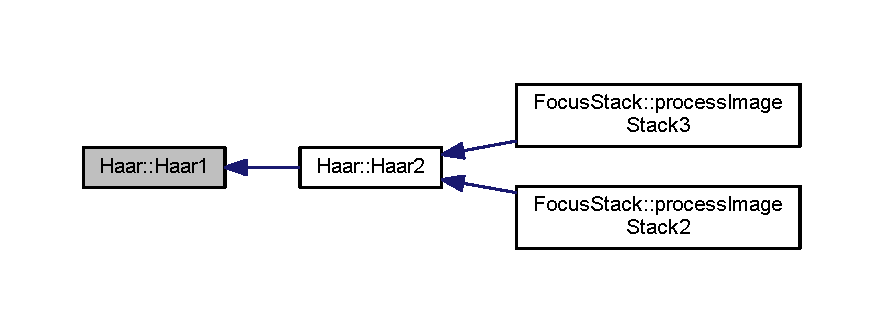
\includegraphics[width=350pt]{class_haar_a44ab3d3043f2a9c2145629a242e6ed0f_icgraph}
\end{center}
\end{figure}
\mbox{\Hypertarget{class_haar_afde8fa7a1d65b505185a29fc7eaf4b2d}\label{class_haar_afde8fa7a1d65b505185a29fc7eaf4b2d}} 
\index{Haar@{Haar}!Haar2@{Haar2}}
\index{Haar2@{Haar2}!Haar@{Haar}}
\subsubsection{\texorpdfstring{Haar2()}{Haar2()}\hspace{0.1cm}{\footnotesize\ttfamily [1/2]}}
{\footnotesize\ttfamily void Haar\+::\+Haar2 (\begin{DoxyParamCaption}\item[{cv\+::\+Mat \&}]{data,  }\item[{int}]{iterations }\end{DoxyParamCaption})\hspace{0.3cm}{\ttfamily [static]}}

Perform 2D \hyperlink{class_haar}{Haar} wavelet pyramid transform with Open\+CV image

\begin{DoxyAuthor}{Author}
David Watts 
\end{DoxyAuthor}
\begin{DoxySince}{Since}
2017/03/08
\end{DoxySince}
Full\+Name \hyperlink{class_haar_afde8fa7a1d65b505185a29fc7eaf4b2d}{Haar\+::\+Haar2} Qualifier 
\begin{DoxyParams}{Parameters}
{\em cv\+::\+Mat} & \& data \\
\hline
{\em int} & iterations (no of levels) \\
\hline
\end{DoxyParams}
\begin{DoxyReturn}{Returns}
void Access private 
\end{DoxyReturn}


Definition at line 214 of file haar.\+cpp.

Here is the call graph for this function\+:
\nopagebreak
\begin{figure}[H]
\begin{center}
\leavevmode
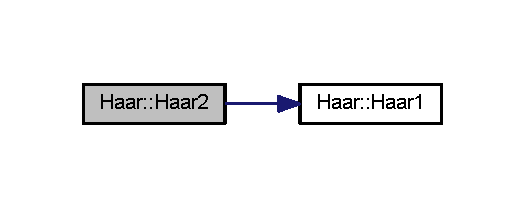
\includegraphics[width=252pt]{class_haar_afde8fa7a1d65b505185a29fc7eaf4b2d_cgraph}
\end{center}
\end{figure}
Here is the caller graph for this function\+:
\nopagebreak
\begin{figure}[H]
\begin{center}
\leavevmode
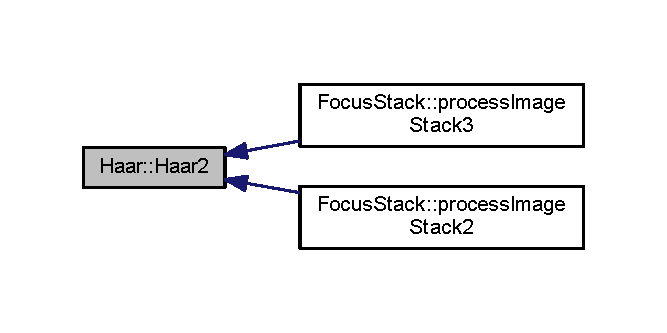
\includegraphics[width=320pt]{class_haar_afde8fa7a1d65b505185a29fc7eaf4b2d_icgraph}
\end{center}
\end{figure}
\mbox{\Hypertarget{class_haar_a4b2951fd5ec6f760fc94bd4273e2c544}\label{class_haar_a4b2951fd5ec6f760fc94bd4273e2c544}} 
\index{Haar@{Haar}!Haar2@{Haar2}}
\index{Haar2@{Haar2}!Haar@{Haar}}
\subsubsection{\texorpdfstring{Haar2()}{Haar2()}\hspace{0.1cm}{\footnotesize\ttfamily [2/2]}}
{\footnotesize\ttfamily template$<$class T $>$ \\
static void Haar\+::\+Haar2 (\begin{DoxyParamCaption}\item[{T $\ast$}]{data,  }\item[{int}]{width,  }\item[{int}]{height,  }\item[{int}]{iterations,  }\item[{bool}]{Abs\+Image = {\ttfamily false} }\end{DoxyParamCaption})\hspace{0.3cm}{\ttfamily [inline]}, {\ttfamily [static]}}

Perform 1D \hyperlink{class_haar}{Haar} wavelet transform on 1D image

\begin{DoxyAuthor}{Author}
David Watts 
\end{DoxyAuthor}
\begin{DoxySince}{Since}
2017/03/08
\end{DoxySince}
Full\+Name \hyperlink{class_haar_afde8fa7a1d65b505185a29fc7eaf4b2d}{Haar\+::\+Haar2} Qualifier 
\begin{DoxyParams}{Parameters}
{\em T} & $\ast$ data \\
\hline
{\em int} & width \\
\hline
{\em int} & height \\
\hline
{\em int} & iterations \\
\hline
{\em bool} & Abs\+Image \\
\hline
\end{DoxyParams}
\begin{DoxyReturn}{Returns}
void Access private 
\end{DoxyReturn}


Definition at line 297 of file haar.\+h.

Here is the call graph for this function\+:
\nopagebreak
\begin{figure}[H]
\begin{center}
\leavevmode
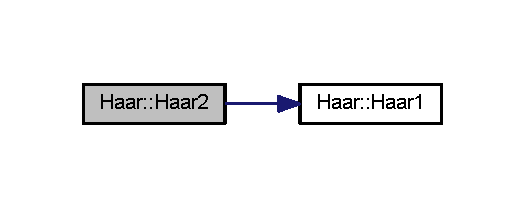
\includegraphics[width=252pt]{class_haar_a4b2951fd5ec6f760fc94bd4273e2c544_cgraph}
\end{center}
\end{figure}
\mbox{\Hypertarget{class_haar_afa323789e73c94995eba32e09d9aa026}\label{class_haar_afa323789e73c94995eba32e09d9aa026}} 
\index{Haar@{Haar}!Haar\+Energy@{Haar\+Energy}}
\index{Haar\+Energy@{Haar\+Energy}!Haar@{Haar}}
\subsubsection{\texorpdfstring{Haar\+Energy()}{HaarEnergy()}}
{\footnotesize\ttfamily void Haar\+::\+Haar\+Energy (\begin{DoxyParamCaption}\item[{cv\+::\+Mat}]{data,  }\item[{cv\+::\+Mat \&}]{energy\+Image,  }\item[{int}]{width,  }\item[{int}]{height,  }\item[{int}]{iterations,  }\item[{bool}]{laplace = {\ttfamily false},  }\item[{bool}]{b\+Square = {\ttfamily true} }\end{DoxyParamCaption})\hspace{0.3cm}{\ttfamily [static]}}

Get energy image (summed coefficient magnitude) from haar wavelet pyramid

\begin{DoxyAuthor}{Author}
David Watts 
\end{DoxyAuthor}
\begin{DoxySince}{Since}
2017/03/08
\end{DoxySince}
Full\+Name \hyperlink{class_haar_afa323789e73c94995eba32e09d9aa026}{Haar\+::\+Haar\+Energy} Qualifier 
\begin{DoxyParams}{Parameters}
{\em cv\+::\+Mat} & data \\
\hline
{\em cv\+::\+Mat} & \& energy\+Image \\
\hline
{\em int} & width \\
\hline
{\em int} & height \\
\hline
{\em int} & iterations \\
\hline
{\em bool} & laplace \\
\hline
{\em bool} & b\+Square \\
\hline
\end{DoxyParams}
\begin{DoxyReturn}{Returns}
void Access private 
\end{DoxyReturn}


Definition at line 29 of file haar.\+cpp.

Here is the caller graph for this function\+:
\nopagebreak
\begin{figure}[H]
\begin{center}
\leavevmode
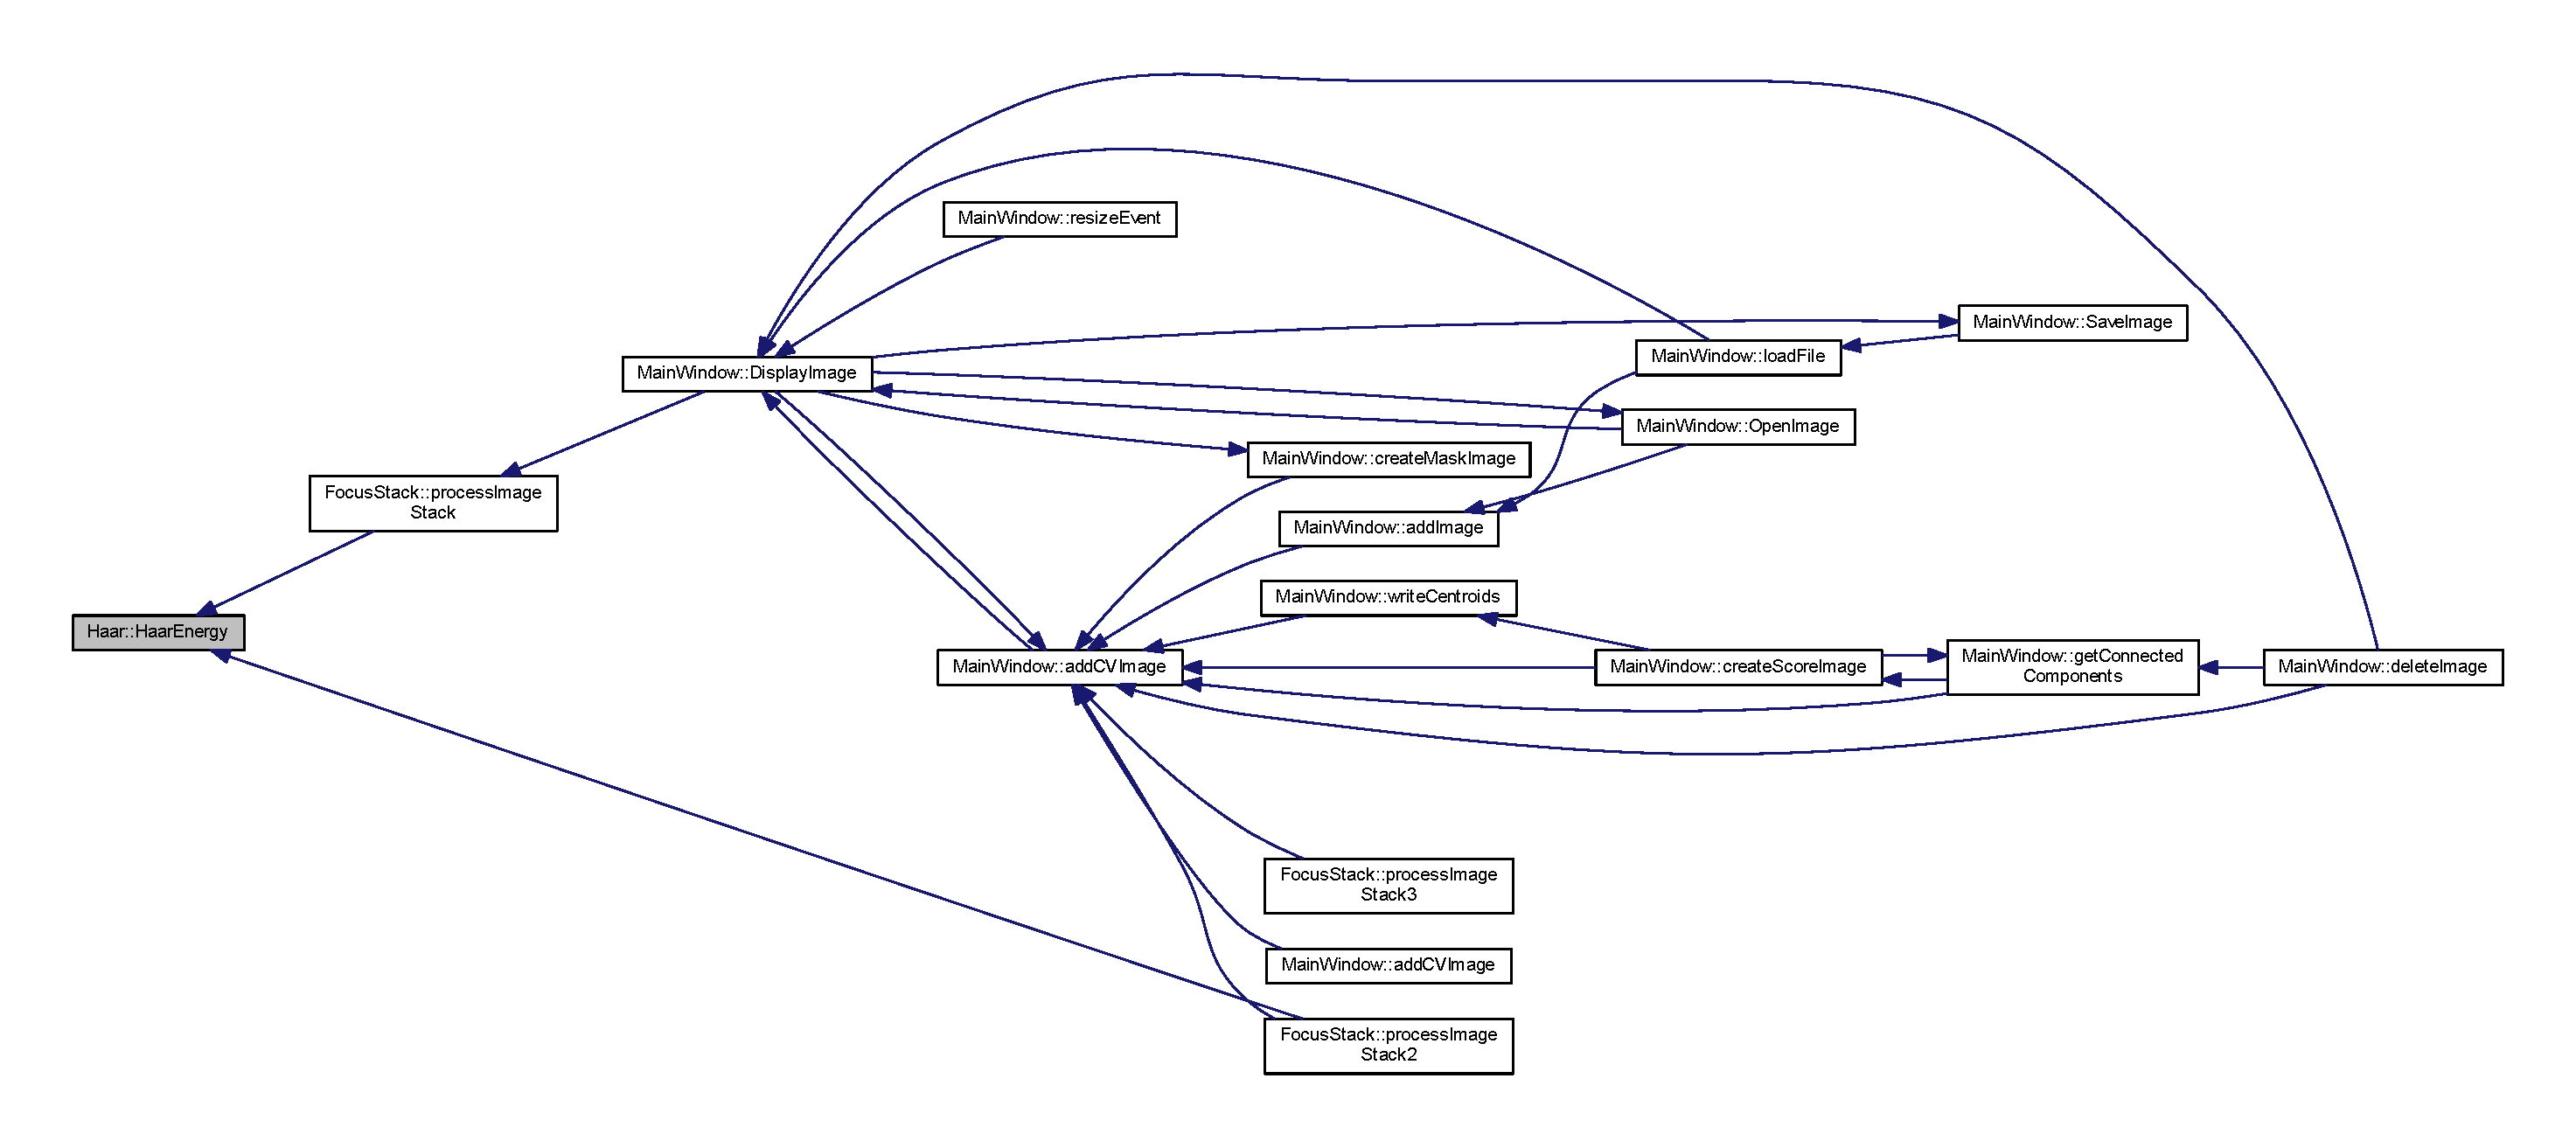
\includegraphics[width=350pt]{class_haar_afa323789e73c94995eba32e09d9aa026_icgraph}
\end{center}
\end{figure}
\mbox{\Hypertarget{class_haar_aedd7102138b5f942b7fbd539b1ff8143}\label{class_haar_aedd7102138b5f942b7fbd539b1ff8143}} 
\index{Haar@{Haar}!i\+Haar1@{i\+Haar1}}
\index{i\+Haar1@{i\+Haar1}!Haar@{Haar}}
\subsubsection{\texorpdfstring{i\+Haar1()}{iHaar1()}}
{\footnotesize\ttfamily template$<$class T $>$ \\
static void Haar\+::i\+Haar1 (\begin{DoxyParamCaption}\item[{T $\ast$}]{data,  }\item[{int}]{n }\end{DoxyParamCaption})\hspace{0.3cm}{\ttfamily [inline]}, {\ttfamily [static]}}

Perform inverse \hyperlink{class_haar}{Haar} wavelet transform on 1D image

\begin{DoxyAuthor}{Author}
David Watts 
\end{DoxyAuthor}
\begin{DoxySince}{Since}
2017/03/08
\end{DoxySince}
Full\+Name \hyperlink{class_haar_aedd7102138b5f942b7fbd539b1ff8143}{Haar\+::i\+Haar1} Qualifier 
\begin{DoxyParams}{Parameters}
{\em T} & $\ast$ data \\
\hline
{\em int} & n \\
\hline
\end{DoxyParams}
\begin{DoxyReturn}{Returns}
void Access private 
\end{DoxyReturn}


Definition at line 422 of file haar.\+h.

Here is the caller graph for this function\+:
\nopagebreak
\begin{figure}[H]
\begin{center}
\leavevmode
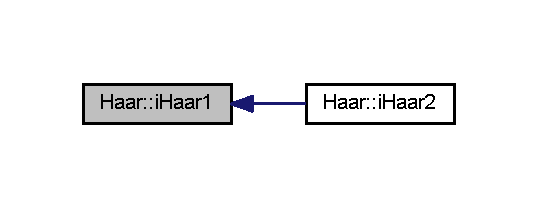
\includegraphics[width=258pt]{class_haar_aedd7102138b5f942b7fbd539b1ff8143_icgraph}
\end{center}
\end{figure}
\mbox{\Hypertarget{class_haar_ab2c372ee9f5eec084066ba52de18fbbe}\label{class_haar_ab2c372ee9f5eec084066ba52de18fbbe}} 
\index{Haar@{Haar}!i\+Haar2@{i\+Haar2}}
\index{i\+Haar2@{i\+Haar2}!Haar@{Haar}}
\subsubsection{\texorpdfstring{i\+Haar2()}{iHaar2()}\hspace{0.1cm}{\footnotesize\ttfamily [1/2]}}
{\footnotesize\ttfamily template$<$class T $>$ \\
static void Haar\+::i\+Haar2 (\begin{DoxyParamCaption}\item[{T $\ast$}]{data,  }\item[{int}]{width,  }\item[{int}]{height,  }\item[{int}]{iterations }\end{DoxyParamCaption})\hspace{0.3cm}{\ttfamily [inline]}, {\ttfamily [static]}}

Perform inverse \hyperlink{class_haar}{Haar} wavelet transform on 2D image

\begin{DoxyAuthor}{Author}
David Watts 
\end{DoxyAuthor}
\begin{DoxySince}{Since}
2017/03/08
\end{DoxySince}
Full\+Name \hyperlink{class_haar_ab2c372ee9f5eec084066ba52de18fbbe}{Haar\+::i\+Haar2} Qualifier 
\begin{DoxyParams}{Parameters}
{\em T} & $\ast$ data \\
\hline
{\em int} & width \\
\hline
{\em int} & height \\
\hline
{\em int} & iterations \\
\hline
\end{DoxyParams}
\begin{DoxyReturn}{Returns}
void Access private 
\end{DoxyReturn}


Definition at line 363 of file haar.\+h.

Here is the call graph for this function\+:
\nopagebreak
\begin{figure}[H]
\begin{center}
\leavevmode
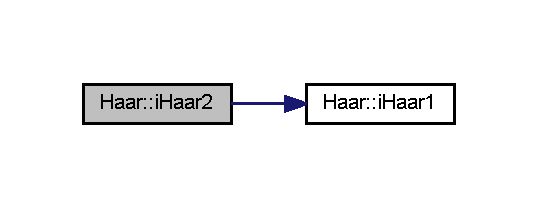
\includegraphics[width=258pt]{class_haar_ab2c372ee9f5eec084066ba52de18fbbe_cgraph}
\end{center}
\end{figure}
\mbox{\Hypertarget{class_haar_a4516357f347f25499ac6aebb717e4f48}\label{class_haar_a4516357f347f25499ac6aebb717e4f48}} 
\index{Haar@{Haar}!i\+Haar2@{i\+Haar2}}
\index{i\+Haar2@{i\+Haar2}!Haar@{Haar}}
\subsubsection{\texorpdfstring{i\+Haar2()}{iHaar2()}\hspace{0.1cm}{\footnotesize\ttfamily [2/2]}}
{\footnotesize\ttfamily template$<$class T $>$ \\
static void Haar\+::i\+Haar2 (\begin{DoxyParamCaption}\item[{cv\+::\+Mat \&}]{data,  }\item[{int}]{iterations }\end{DoxyParamCaption})\hspace{0.3cm}{\ttfamily [inline]}, {\ttfamily [static]}}

Perform inverse \hyperlink{class_haar}{Haar} wavelet transform on 2D Open\+CV image

\begin{DoxyAuthor}{Author}
David Watts 
\end{DoxyAuthor}
\begin{DoxySince}{Since}
2017/03/08
\end{DoxySince}
Full\+Name \hyperlink{class_haar_ab2c372ee9f5eec084066ba52de18fbbe}{Haar\+::i\+Haar2} Qualifier 
\begin{DoxyParams}{Parameters}
{\em cv\+::\+Mat} & \& data \\
\hline
{\em int} & iterations \\
\hline
\end{DoxyParams}
\begin{DoxyReturn}{Returns}
void Access private 
\end{DoxyReturn}


Definition at line 455 of file haar.\+h.

Here is the call graph for this function\+:
\nopagebreak
\begin{figure}[H]
\begin{center}
\leavevmode
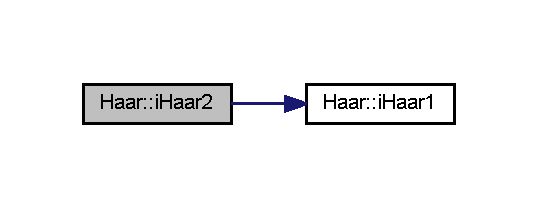
\includegraphics[width=258pt]{class_haar_a4516357f347f25499ac6aebb717e4f48_cgraph}
\end{center}
\end{figure}
\mbox{\Hypertarget{class_haar_ad85443bf4bbe9d65be10acbd0d89093b}\label{class_haar_ad85443bf4bbe9d65be10acbd0d89093b}} 
\index{Haar@{Haar}!Laplacian\+Pyramid@{Laplacian\+Pyramid}}
\index{Laplacian\+Pyramid@{Laplacian\+Pyramid}!Haar@{Haar}}
\subsubsection{\texorpdfstring{Laplacian\+Pyramid()}{LaplacianPyramid()}}
{\footnotesize\ttfamily cv\+::\+Mat Haar\+::\+Laplacian\+Pyramid (\begin{DoxyParamCaption}\item[{cv\+::\+Mat}]{im,  }\item[{int}]{levels,  }\item[{bool}]{include\+Scale = {\ttfamily true} }\end{DoxyParamCaption})\hspace{0.3cm}{\ttfamily [static]}}

perform Laplacian pyramid

\begin{DoxyAuthor}{Author}
David Watts 
\end{DoxyAuthor}
\begin{DoxySince}{Since}
2017/03/08
\end{DoxySince}
Full\+Name \hyperlink{class_haar_ad85443bf4bbe9d65be10acbd0d89093b}{Haar\+::\+Laplacian\+Pyramid} Qualifier 
\begin{DoxyParams}{Parameters}
{\em cv\+::\+Mat} & im \\
\hline
{\em int} & levels \\
\hline
{\em bool} & include\+Scale \\
\hline
\end{DoxyParams}
\begin{DoxyReturn}{Returns}
cv\+::\+Mat Access private 
\end{DoxyReturn}


Definition at line 81 of file haar.\+cpp.

Here is the caller graph for this function\+:
\nopagebreak
\begin{figure}[H]
\begin{center}
\leavevmode
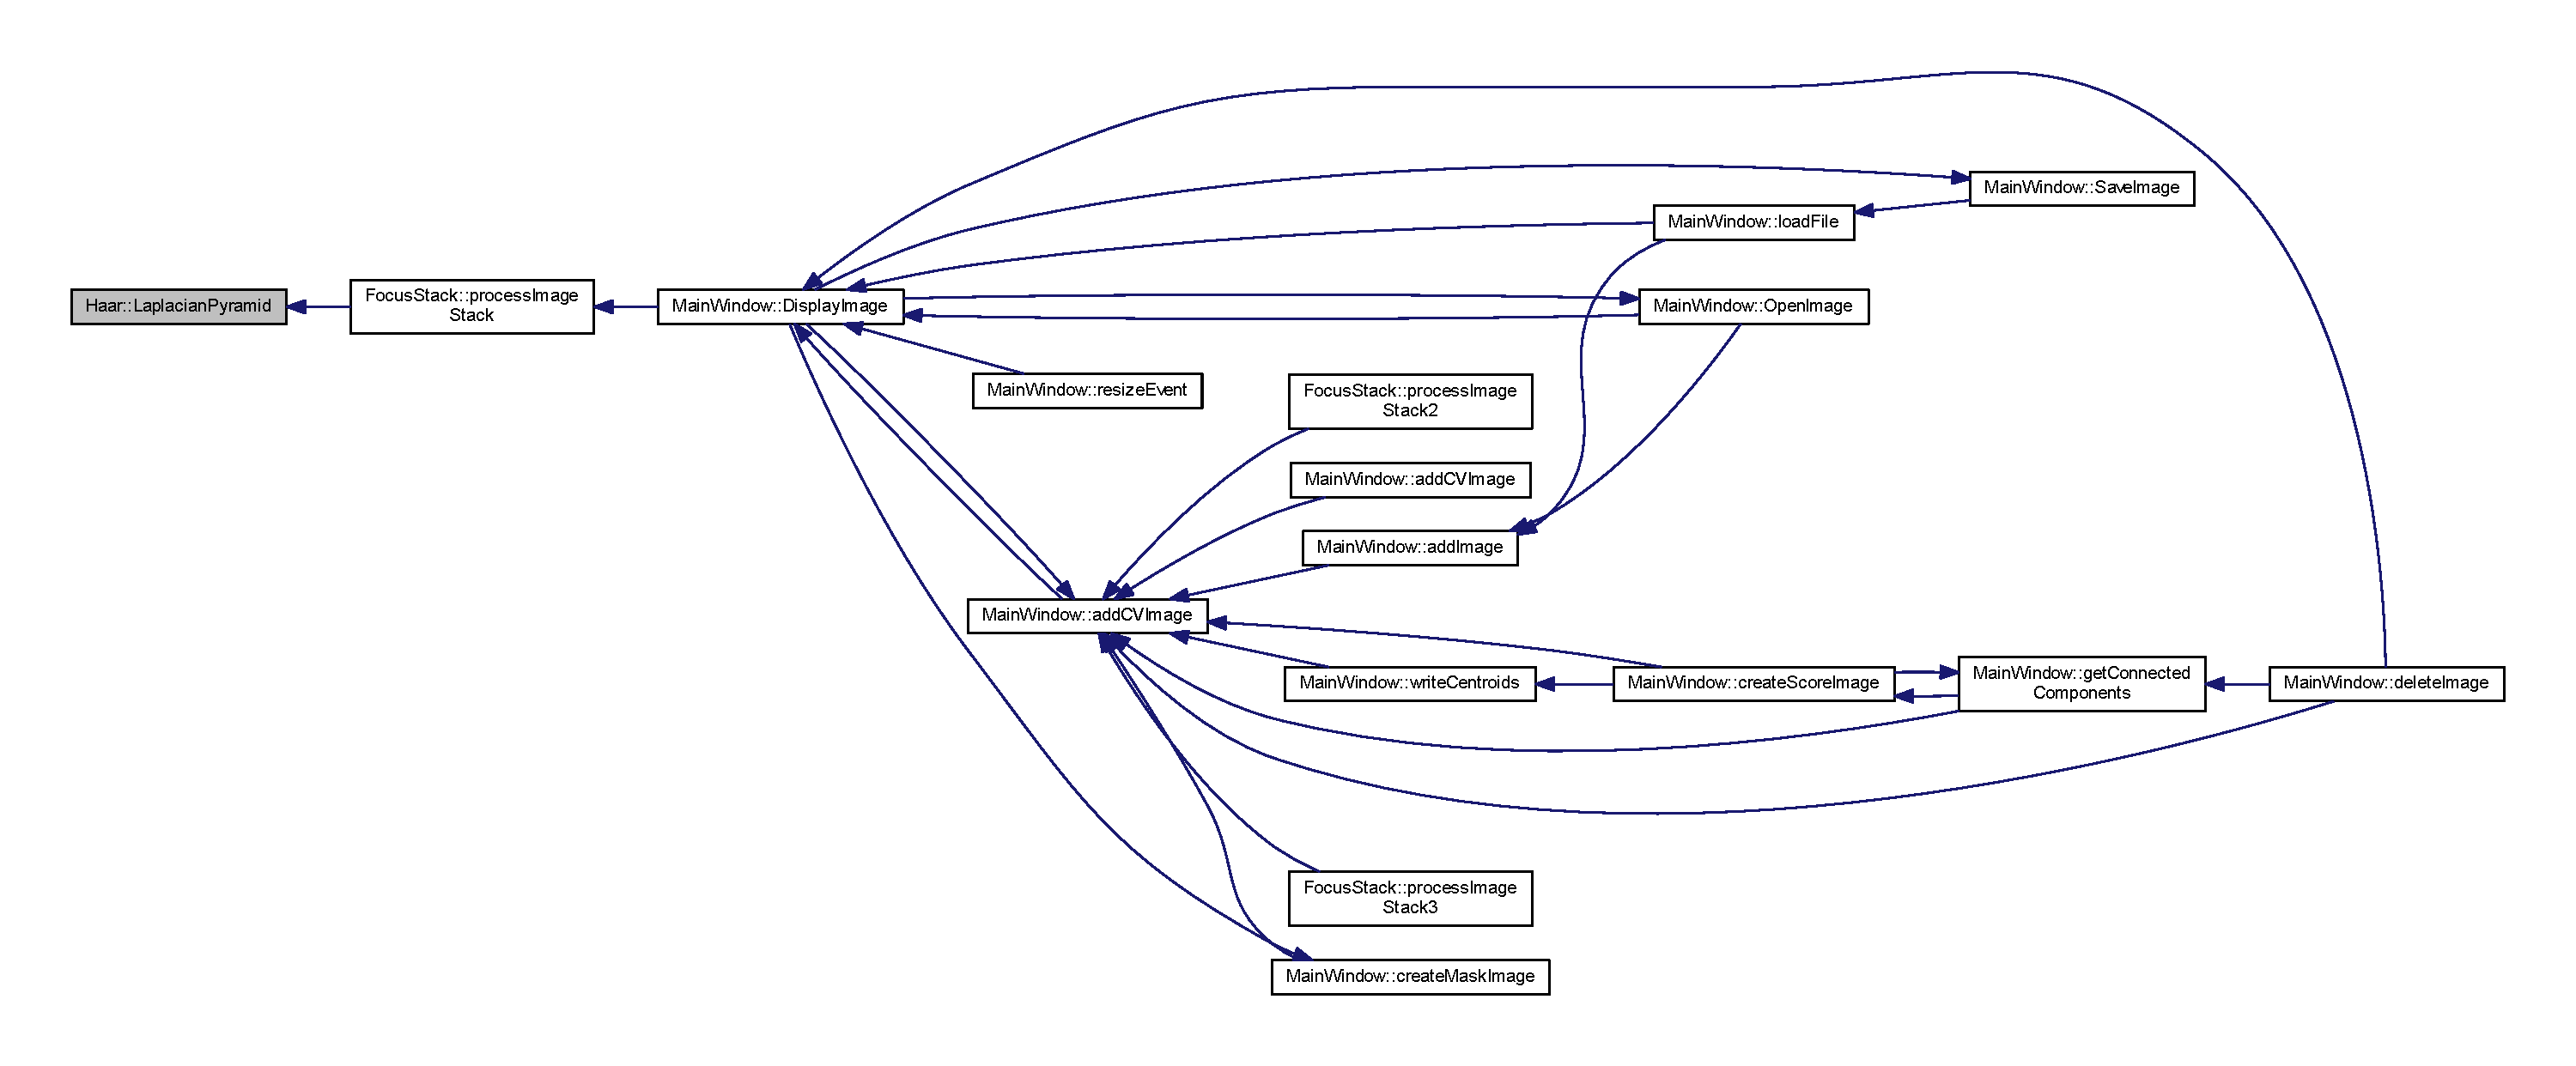
\includegraphics[width=350pt]{class_haar_ad85443bf4bbe9d65be10acbd0d89093b_icgraph}
\end{center}
\end{figure}
\mbox{\Hypertarget{class_haar_a5a0726cb9e3a28295ba4ac64f654aa36}\label{class_haar_a5a0726cb9e3a28295ba4ac64f654aa36}} 
\index{Haar@{Haar}!Pyramid\+Levels@{Pyramid\+Levels}}
\index{Pyramid\+Levels@{Pyramid\+Levels}!Haar@{Haar}}
\subsubsection{\texorpdfstring{Pyramid\+Levels()}{PyramidLevels()}\hspace{0.1cm}{\footnotesize\ttfamily [1/2]}}
{\footnotesize\ttfamily cv\+::\+Mat Haar\+::\+Pyramid\+Levels (\begin{DoxyParamCaption}\item[{cv\+::\+Mat}]{data,  }\item[{int}]{width,  }\item[{int}]{height,  }\item[{int}]{iterations,  }\item[{const int}]{No\+Focus\+Images }\end{DoxyParamCaption})\hspace{0.3cm}{\ttfamily [static]}}

Get Open\+CV image of best (modal) values from Pyramid composition

\begin{DoxyAuthor}{Author}
David Watts 
\end{DoxyAuthor}
\begin{DoxySince}{Since}
2017/03/08
\end{DoxySince}
Full\+Name \hyperlink{class_haar_a5a0726cb9e3a28295ba4ac64f654aa36}{Haar\+::\+Pyramid\+Levels} Qualifier 
\begin{DoxyParams}{Parameters}
{\em cv\+::\+Mat} & data \\
\hline
{\em int} & width \\
\hline
{\em int} & height \\
\hline
{\em int} & iterations \\
\hline
{\em const} & int No\+Focus\+Images \\
\hline
\end{DoxyParams}
\begin{DoxyReturn}{Returns}
cv\+::\+Mat Access private 
\end{DoxyReturn}


Definition at line 139 of file haar.\+cpp.

Here is the caller graph for this function\+:
\nopagebreak
\begin{figure}[H]
\begin{center}
\leavevmode
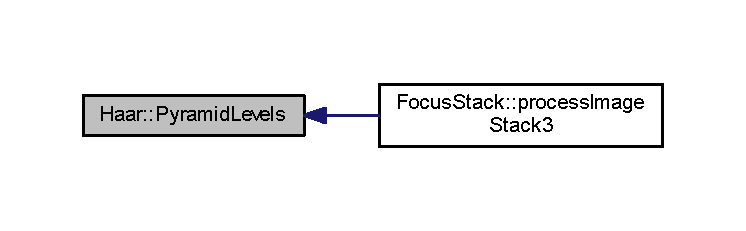
\includegraphics[width=350pt]{class_haar_a5a0726cb9e3a28295ba4ac64f654aa36_icgraph}
\end{center}
\end{figure}
\mbox{\Hypertarget{class_haar_a6724557f8d0a1660df2a9de85d7ce523}\label{class_haar_a6724557f8d0a1660df2a9de85d7ce523}} 
\index{Haar@{Haar}!Pyramid\+Levels@{Pyramid\+Levels}}
\index{Pyramid\+Levels@{Pyramid\+Levels}!Haar@{Haar}}
\subsubsection{\texorpdfstring{Pyramid\+Levels()}{PyramidLevels()}\hspace{0.1cm}{\footnotesize\ttfamily [2/2]}}
{\footnotesize\ttfamily template$<$class T $>$ \\
static T$\ast$ Haar\+::\+Pyramid\+Levels (\begin{DoxyParamCaption}\item[{T $\ast$}]{data,  }\item[{int}]{width,  }\item[{int}]{height,  }\item[{int}]{iterations,  }\item[{int}]{No\+Focus\+Images }\end{DoxyParamCaption})\hspace{0.3cm}{\ttfamily [inline]}, {\ttfamily [static]}}

Get image of best (modal) values from Pyramid composition

\begin{DoxyAuthor}{Author}
David Watts 
\end{DoxyAuthor}
\begin{DoxySince}{Since}
2017/03/08
\end{DoxySince}
Full\+Name \hyperlink{class_haar_a5a0726cb9e3a28295ba4ac64f654aa36}{Haar\+::\+Pyramid\+Levels} Qualifier 
\begin{DoxyParams}{Parameters}
{\em T} & $\ast$ data \\
\hline
{\em int} & width \\
\hline
{\em int} & height \\
\hline
{\em int} & iterations \\
\hline
{\em int} & No\+Focus\+Images \\
\hline
\end{DoxyParams}
\begin{DoxyReturn}{Returns}
T$\ast$ Access private 
\end{DoxyReturn}


Definition at line 44 of file haar.\+h.

\mbox{\Hypertarget{class_haar_a4f48761ec2f91c74df7ef6b501238d2a}\label{class_haar_a4f48761ec2f91c74df7ef6b501238d2a}} 
\index{Haar@{Haar}!Pyramid\+Region\+Levels@{Pyramid\+Region\+Levels}}
\index{Pyramid\+Region\+Levels@{Pyramid\+Region\+Levels}!Haar@{Haar}}
\subsubsection{\texorpdfstring{Pyramid\+Region\+Levels()}{PyramidRegionLevels()}}
{\footnotesize\ttfamily template$<$class T $>$ \\
static T$\ast$ Haar\+::\+Pyramid\+Region\+Levels (\begin{DoxyParamCaption}\item[{T $\ast$}]{data,  }\item[{int}]{width,  }\item[{int}]{height,  }\item[{int}]{iterations,  }\item[{int}]{No\+Focus\+Images }\end{DoxyParamCaption})\hspace{0.3cm}{\ttfamily [inline]}, {\ttfamily [static]}}

Get image of best (modal) values from local 8 connected neighbours of Pyramid composition

\begin{DoxyAuthor}{Author}
David Watts 
\end{DoxyAuthor}
\begin{DoxySince}{Since}
2017/03/08
\end{DoxySince}
Full\+Name \hyperlink{class_haar_a4f48761ec2f91c74df7ef6b501238d2a}{Haar\+::\+Pyramid\+Region\+Levels} Qualifier 
\begin{DoxyParams}{Parameters}
{\em T} & $\ast$ data \\
\hline
{\em int} & width \\
\hline
{\em int} & height \\
\hline
{\em int} & iterations \\
\hline
{\em int} & No\+Focus\+Images \\
\hline
\end{DoxyParams}
\begin{DoxyReturn}{Returns}
T$\ast$ Access private 
\end{DoxyReturn}


Definition at line 122 of file haar.\+h.



The documentation for this class was generated from the following files\+:\begin{DoxyCompactItemize}
\item 
H\+:/\+Code\+Projects/\+Q\+T\+Projects/\+Targeter-\/msvc/haar.\+h\item 
H\+:/\+Code\+Projects/\+Q\+T\+Projects/\+Targeter-\/msvc/haar.\+hpp\item 
H\+:/\+Code\+Projects/\+Q\+T\+Projects/\+Targeter-\/msvc/haar.\+cpp\end{DoxyCompactItemize}

\hypertarget{class_helper_functions}{}\section{Helper\+Functions Class Reference}
\label{class_helper_functions}\index{Helper\+Functions@{Helper\+Functions}}


{\ttfamily \#include $<$Helper\+Functions.\+h$>$}



Collaboration diagram for Helper\+Functions\+:
\nopagebreak
\begin{figure}[H]
\begin{center}
\leavevmode
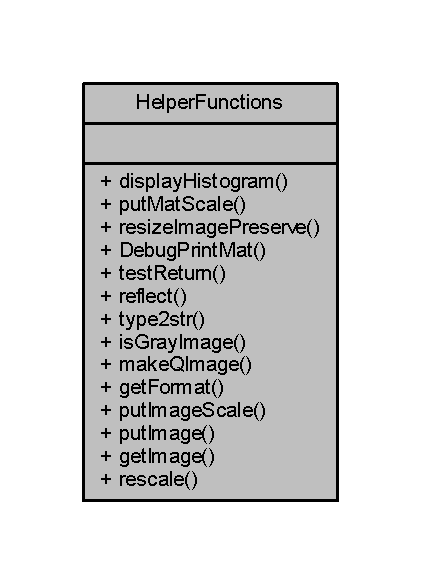
\includegraphics[width=202pt]{class_helper_functions__coll__graph}
\end{center}
\end{figure}
\subsection*{Static Public Member Functions}
\begin{DoxyCompactItemize}
\item 
static cv\+::\+Mat \hyperlink{class_helper_functions_a5c5283b1bdbfff78c4381a93161effe5}{display\+Histogram} (int hist\+Size, cv\+::\+Mat b\+\_\+hist, int hist\+\_\+w=512, int hist\+\_\+h=400)
\item 
static cv\+::\+Mat \hyperlink{class_helper_functions_ad960d64773884aa54332b6b72ab5b876}{put\+Mat\+Scale} (cv\+::\+Mat im, bool scale=true, bool b\+Red=true)
\item 
static void \hyperlink{class_helper_functions_a7afac4bb91186ab522a3a1d640589e7e}{resize\+Image\+Preserve} (cv\+::\+Mat \&image\+In, cv\+::\+Mat \&image\+Out, int new\+Width, int new\+Height)
\item 
static void \hyperlink{class_helper_functions_a375b456c83eb7d8b7746a700e1ec38d1}{Debug\+Print\+Mat} (cv\+::\+Mat mat)
\item 
\mbox{\Hypertarget{class_helper_functions_a9f86f713dcf72f162c085e88e26c9d08}\label{class_helper_functions_a9f86f713dcf72f162c085e88e26c9d08}} 
static cv\+::\+Mat {\bfseries test\+Return} (cv\+::\+Mat \&im)
\item 
static int \hyperlink{class_helper_functions_af83ef83dc647e660335bf5564f5fdda7}{reflect} (int M, int x)
\item 
static std\+::string \hyperlink{class_helper_functions_a0b9d882eaf6b7d85aad907ee3e94d197}{type2str} (int type)
\item 
static bool \hyperlink{class_helper_functions_aa04bae06c901791851f8d84607927001}{is\+Gray\+Image} (cv\+::\+Mat img)
\item 
static Q\+Image \hyperlink{class_helper_functions_a905e9fa464584f31d1537a84d8d348ae}{make\+Q\+Image} (cv\+::\+Mat im, bool b\+R\+G\+B\+Swap=true)
\item 
static Q\+Image\+::\+Format \hyperlink{class_helper_functions_a64c4fa7fceb347bc87600d926ab9a6dc}{get\+Format} (int type)
\item 
{\footnotesize template$<$typename T $>$ }\\static cv\+::\+Mat \hyperlink{class_helper_functions_a3bd3b4664ce50153abfb3b75a6fc51ba}{put\+Image\+Scale} (T $\ast$im, int w, int h)
\item 
{\footnotesize template$<$typename T $>$ }\\static cv\+::\+Mat \hyperlink{class_helper_functions_ae2a270fba6b59601060ec8ab2e338cc1}{put\+Image} (T $\ast$im, int width, int height)
\item 
{\footnotesize template$<$typename T $>$ }\\static T $\ast$ \hyperlink{class_helper_functions_a1d33065de9de137025c132c3c9766130}{get\+Image} (cv\+::\+Mat \&m)
\item 
{\footnotesize template$<$typename T $>$ }\\static void \hyperlink{class_helper_functions_a7807daf795fa0056e924f191be8abaf9}{rescale} (T $\ast$im, int w, int h)
\end{DoxyCompactItemize}


\subsection{Detailed Description}
class for useful helper image manipulation functions 

Definition at line 11 of file Helper\+Functions.\+h.



\subsection{Member Function Documentation}
\mbox{\Hypertarget{class_helper_functions_a375b456c83eb7d8b7746a700e1ec38d1}\label{class_helper_functions_a375b456c83eb7d8b7746a700e1ec38d1}} 
\index{Helper\+Functions@{Helper\+Functions}!Debug\+Print\+Mat@{Debug\+Print\+Mat}}
\index{Debug\+Print\+Mat@{Debug\+Print\+Mat}!Helper\+Functions@{Helper\+Functions}}
\subsubsection{\texorpdfstring{Debug\+Print\+Mat()}{DebugPrintMat()}}
{\footnotesize\ttfamily void Helper\+Functions\+::\+Debug\+Print\+Mat (\begin{DoxyParamCaption}\item[{cv\+::\+Mat}]{mat }\end{DoxyParamCaption})\hspace{0.3cm}{\ttfamily [static]}}

prints 2D matrix to screen

\begin{DoxyAuthor}{Author}
David Watts 
\end{DoxyAuthor}
\begin{DoxySince}{Since}
2017/03/07
\end{DoxySince}
Full\+Name \hyperlink{class_helper_functions_a375b456c83eb7d8b7746a700e1ec38d1}{Helper\+Functions\+::\+Debug\+Print\+Mat} Qualifier 
\begin{DoxyParams}{Parameters}
{\em cv\+::\+Mat} & mat \\
\hline
\end{DoxyParams}
\begin{DoxyReturn}{Returns}
void Access public 
\end{DoxyReturn}


Definition at line 342 of file Helper\+Functions.\+cpp.

\mbox{\Hypertarget{class_helper_functions_a5c5283b1bdbfff78c4381a93161effe5}\label{class_helper_functions_a5c5283b1bdbfff78c4381a93161effe5}} 
\index{Helper\+Functions@{Helper\+Functions}!display\+Histogram@{display\+Histogram}}
\index{display\+Histogram@{display\+Histogram}!Helper\+Functions@{Helper\+Functions}}
\subsubsection{\texorpdfstring{display\+Histogram()}{displayHistogram()}}
{\footnotesize\ttfamily cv\+::\+Mat Helper\+Functions\+::display\+Histogram (\begin{DoxyParamCaption}\item[{int}]{hist\+Size,  }\item[{cv\+::\+Mat}]{b\+\_\+hist,  }\item[{int}]{hist\+\_\+w = {\ttfamily 512},  }\item[{int}]{hist\+\_\+h = {\ttfamily 400} }\end{DoxyParamCaption})\hspace{0.3cm}{\ttfamily [static]}}

Returns an Open\+CV image from a histogram (b\+\_\+hist)

\begin{DoxyAuthor}{Author}
David Watts 
\end{DoxyAuthor}
\begin{DoxySince}{Since}
2017/03/07
\end{DoxySince}
Full\+Name \hyperlink{class_helper_functions_a5c5283b1bdbfff78c4381a93161effe5}{Helper\+Functions\+::display\+Histogram} Qualifier 
\begin{DoxyParams}{Parameters}
{\em int} & hist\+Size \\
\hline
{\em cv\+::\+Mat} & b\+\_\+hist \\
\hline
{\em int} & hist\+\_\+w \\
\hline
{\em int} & hist\+\_\+h \\
\hline
\end{DoxyParams}
\begin{DoxyReturn}{Returns}
cv\+::\+Mat Access public 
\end{DoxyReturn}
Draw for each channel

Draw for each channel 

Definition at line 71 of file Helper\+Functions.\+cpp.

Here is the caller graph for this function\+:
\nopagebreak
\begin{figure}[H]
\begin{center}
\leavevmode
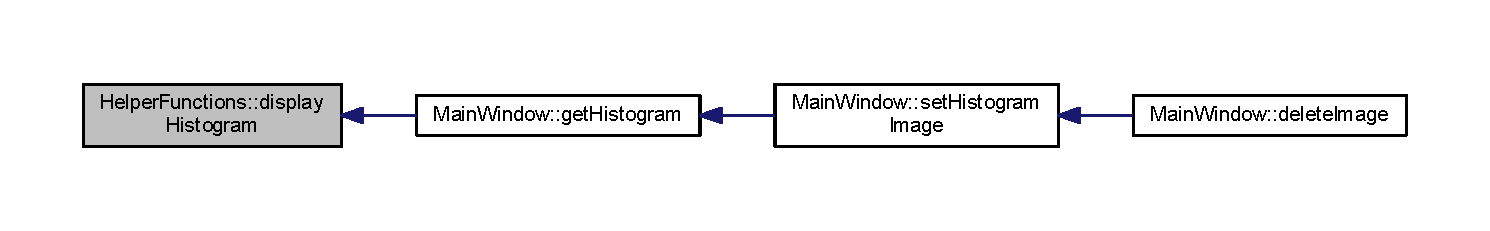
\includegraphics[width=350pt]{class_helper_functions_a5c5283b1bdbfff78c4381a93161effe5_icgraph}
\end{center}
\end{figure}
\mbox{\Hypertarget{class_helper_functions_a64c4fa7fceb347bc87600d926ab9a6dc}\label{class_helper_functions_a64c4fa7fceb347bc87600d926ab9a6dc}} 
\index{Helper\+Functions@{Helper\+Functions}!get\+Format@{get\+Format}}
\index{get\+Format@{get\+Format}!Helper\+Functions@{Helper\+Functions}}
\subsubsection{\texorpdfstring{get\+Format()}{getFormat()}}
{\footnotesize\ttfamily Q\+Image\+::\+Format Helper\+Functions\+::get\+Format (\begin{DoxyParamCaption}\item[{int}]{type }\end{DoxyParamCaption})\hspace{0.3cm}{\ttfamily [static]}}

Returns QT Image type for Open\+CV type

\begin{DoxyAuthor}{Author}
David Watts 
\end{DoxyAuthor}
\begin{DoxySince}{Since}
2017/03/07
\end{DoxySince}
Full\+Name \hyperlink{class_helper_functions_a64c4fa7fceb347bc87600d926ab9a6dc}{Helper\+Functions\+::get\+Format} Qualifier 
\begin{DoxyParams}{Parameters}
{\em int} & type \\
\hline
\end{DoxyParams}
\begin{DoxyReturn}{Returns}
Q\+T\+\_\+\+N\+A\+M\+E\+S\+P\+A\+C\+E\+::\+Q\+Image\+::\+Format Access public 
\end{DoxyReturn}


Definition at line 207 of file Helper\+Functions.\+cpp.

Here is the caller graph for this function\+:
\nopagebreak
\begin{figure}[H]
\begin{center}
\leavevmode
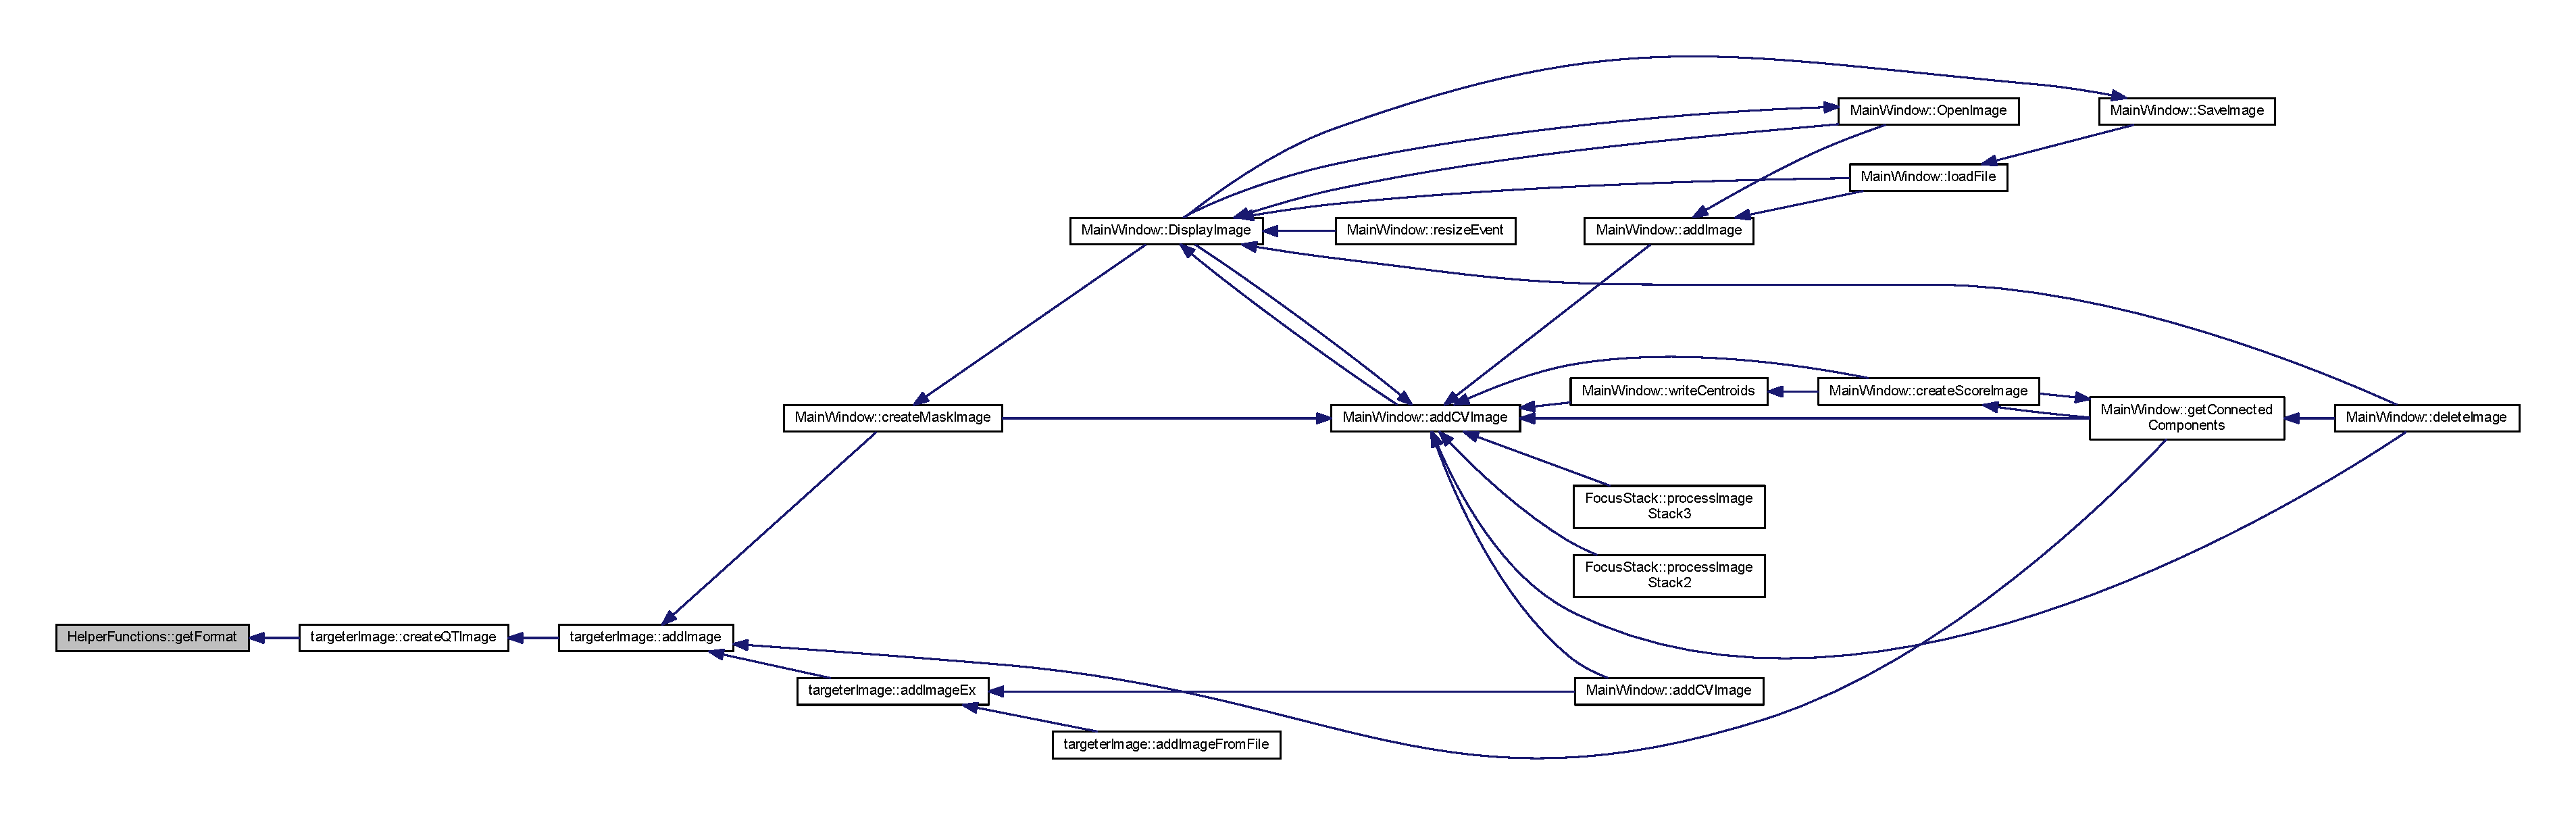
\includegraphics[width=350pt]{class_helper_functions_a64c4fa7fceb347bc87600d926ab9a6dc_icgraph}
\end{center}
\end{figure}
\mbox{\Hypertarget{class_helper_functions_a1d33065de9de137025c132c3c9766130}\label{class_helper_functions_a1d33065de9de137025c132c3c9766130}} 
\index{Helper\+Functions@{Helper\+Functions}!get\+Image@{get\+Image}}
\index{get\+Image@{get\+Image}!Helper\+Functions@{Helper\+Functions}}
\subsubsection{\texorpdfstring{get\+Image()}{getImage()}}
{\footnotesize\ttfamily template$<$typename T $>$ \\
static T$\ast$ Helper\+Functions\+::get\+Image (\begin{DoxyParamCaption}\item[{cv\+::\+Mat \&}]{m }\end{DoxyParamCaption})\hspace{0.3cm}{\ttfamily [inline]}, {\ttfamily [static]}}

Returns a greyscale 1D int$\ast$ image array from an Open\+CV image

\begin{DoxyAuthor}{Author}
David Watts 
\end{DoxyAuthor}
\begin{DoxySince}{Since}
2017/03/07
\end{DoxySince}
Full\+Name \hyperlink{class_helper_functions_a1d33065de9de137025c132c3c9766130}{Helper\+Functions\+::get\+Image} Qualifier 
\begin{DoxyParams}{Parameters}
{\em cv\+::\+Mat} & \& m \\
\hline
\end{DoxyParams}
\begin{DoxyReturn}{Returns}
T$\ast$ Access public 
\end{DoxyReturn}


Definition at line 135 of file Helper\+Functions.\+h.

\mbox{\Hypertarget{class_helper_functions_aa04bae06c901791851f8d84607927001}\label{class_helper_functions_aa04bae06c901791851f8d84607927001}} 
\index{Helper\+Functions@{Helper\+Functions}!is\+Gray\+Image@{is\+Gray\+Image}}
\index{is\+Gray\+Image@{is\+Gray\+Image}!Helper\+Functions@{Helper\+Functions}}
\subsubsection{\texorpdfstring{is\+Gray\+Image()}{isGrayImage()}}
{\footnotesize\ttfamily bool Helper\+Functions\+::is\+Gray\+Image (\begin{DoxyParamCaption}\item[{cv\+::\+Mat}]{img }\end{DoxyParamCaption})\hspace{0.3cm}{\ttfamily [static]}}

determines if image is greyscale

\begin{DoxyAuthor}{Author}
David Watts 
\end{DoxyAuthor}
\begin{DoxySince}{Since}
2017/03/07
\end{DoxySince}
Full\+Name \hyperlink{class_helper_functions_aa04bae06c901791851f8d84607927001}{Helper\+Functions\+::is\+Gray\+Image} Qualifier // returns true if the given 3 channel image is B = G = R 
\begin{DoxyParams}{Parameters}
{\em cv\+::\+Mat} & img \\
\hline
\end{DoxyParams}
\begin{DoxyReturn}{Returns}
bool Access public 
\end{DoxyReturn}


Definition at line 242 of file Helper\+Functions.\+cpp.

\mbox{\Hypertarget{class_helper_functions_a905e9fa464584f31d1537a84d8d348ae}\label{class_helper_functions_a905e9fa464584f31d1537a84d8d348ae}} 
\index{Helper\+Functions@{Helper\+Functions}!make\+Q\+Image@{make\+Q\+Image}}
\index{make\+Q\+Image@{make\+Q\+Image}!Helper\+Functions@{Helper\+Functions}}
\subsubsection{\texorpdfstring{make\+Q\+Image()}{makeQImage()}}
{\footnotesize\ttfamily Q\+Image Helper\+Functions\+::make\+Q\+Image (\begin{DoxyParamCaption}\item[{cv\+::\+Mat}]{im,  }\item[{bool}]{b\+R\+G\+B\+Swap = {\ttfamily true} }\end{DoxyParamCaption})\hspace{0.3cm}{\ttfamily [static]}}

make Q\+Image from Open\+CV image

\begin{DoxyAuthor}{Author}
David Watts 
\end{DoxyAuthor}
\begin{DoxySince}{Since}
2017/03/07
\end{DoxySince}
Full\+Name \hyperlink{class_helper_functions_a905e9fa464584f31d1537a84d8d348ae}{Helper\+Functions\+::make\+Q\+Image} Qualifier 
\begin{DoxyParams}{Parameters}
{\em cv\+::\+Mat} & im \\
\hline
{\em bool} & b\+R\+G\+B\+Swap \\
\hline
\end{DoxyParams}
\begin{DoxyReturn}{Returns}
Q\+T\+\_\+\+N\+A\+M\+E\+S\+P\+A\+C\+E\+::\+Q\+Image Access public 
\end{DoxyReturn}


Definition at line 181 of file Helper\+Functions.\+cpp.

Here is the caller graph for this function\+:
\nopagebreak
\begin{figure}[H]
\begin{center}
\leavevmode
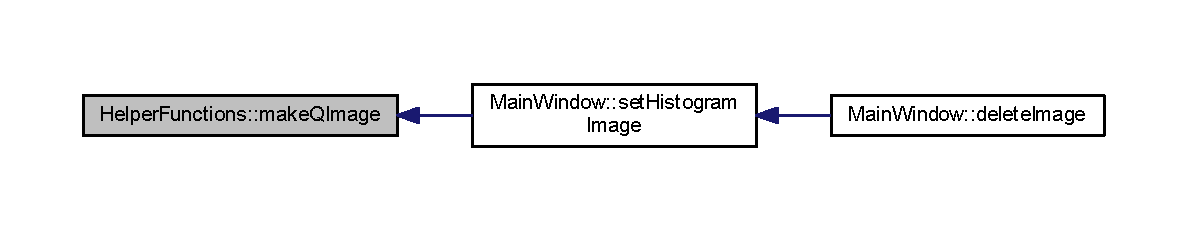
\includegraphics[width=350pt]{class_helper_functions_a905e9fa464584f31d1537a84d8d348ae_icgraph}
\end{center}
\end{figure}
\mbox{\Hypertarget{class_helper_functions_ae2a270fba6b59601060ec8ab2e338cc1}\label{class_helper_functions_ae2a270fba6b59601060ec8ab2e338cc1}} 
\index{Helper\+Functions@{Helper\+Functions}!put\+Image@{put\+Image}}
\index{put\+Image@{put\+Image}!Helper\+Functions@{Helper\+Functions}}
\subsubsection{\texorpdfstring{put\+Image()}{putImage()}}
{\footnotesize\ttfamily template$<$typename T $>$ \\
static cv\+::\+Mat Helper\+Functions\+::put\+Image (\begin{DoxyParamCaption}\item[{T $\ast$}]{im,  }\item[{int}]{width,  }\item[{int}]{height }\end{DoxyParamCaption})\hspace{0.3cm}{\ttfamily [inline]}, {\ttfamily [static]}}

creates a opencv image from int$\ast$ 1D image array

\begin{DoxyAuthor}{Author}
David Watts 
\end{DoxyAuthor}
\begin{DoxySince}{Since}
2017/03/08
\end{DoxySince}
Full\+Name put\+Image Qualifier 
\begin{DoxyParams}{Parameters}
{\em T} & $\ast$ im \\
\hline
{\em int} & width \\
\hline
{\em int} & height \\
\hline
\end{DoxyParams}
\begin{DoxyReturn}{Returns}
cv\+::\+Mat Access public static 
\end{DoxyReturn}


Definition at line 104 of file Helper\+Functions.\+h.

\mbox{\Hypertarget{class_helper_functions_a3bd3b4664ce50153abfb3b75a6fc51ba}\label{class_helper_functions_a3bd3b4664ce50153abfb3b75a6fc51ba}} 
\index{Helper\+Functions@{Helper\+Functions}!put\+Image\+Scale@{put\+Image\+Scale}}
\index{put\+Image\+Scale@{put\+Image\+Scale}!Helper\+Functions@{Helper\+Functions}}
\subsubsection{\texorpdfstring{put\+Image\+Scale()}{putImageScale()}}
{\footnotesize\ttfamily template$<$typename T $>$ \\
static cv\+::\+Mat Helper\+Functions\+::put\+Image\+Scale (\begin{DoxyParamCaption}\item[{T $\ast$}]{im,  }\item[{int}]{w,  }\item[{int}]{h }\end{DoxyParamCaption})\hspace{0.3cm}{\ttfamily [inline]}, {\ttfamily [static]}}

creates a scaled opencv image from int$\ast$ 1D image array

\begin{DoxyAuthor}{Author}
David Watts 
\end{DoxyAuthor}
\begin{DoxySince}{Since}
2017/03/08
\end{DoxySince}
Full\+Name put\+Image\+Scale Qualifier 
\begin{DoxyParams}{Parameters}
{\em T} & $\ast$ im \\
\hline
{\em int} & w \\
\hline
{\em int} & h \\
\hline
\end{DoxyParams}
\begin{DoxyReturn}{Returns}
cv\+::\+Mat Access public static 
\end{DoxyReturn}


Definition at line 51 of file Helper\+Functions.\+h.

\mbox{\Hypertarget{class_helper_functions_ad960d64773884aa54332b6b72ab5b876}\label{class_helper_functions_ad960d64773884aa54332b6b72ab5b876}} 
\index{Helper\+Functions@{Helper\+Functions}!put\+Mat\+Scale@{put\+Mat\+Scale}}
\index{put\+Mat\+Scale@{put\+Mat\+Scale}!Helper\+Functions@{Helper\+Functions}}
\subsubsection{\texorpdfstring{put\+Mat\+Scale()}{putMatScale()}}
{\footnotesize\ttfamily cv\+::\+Mat Helper\+Functions\+::put\+Mat\+Scale (\begin{DoxyParamCaption}\item[{cv\+::\+Mat}]{im,  }\item[{bool}]{scale = {\ttfamily true},  }\item[{bool}]{b\+Red = {\ttfamily true} }\end{DoxyParamCaption})\hspace{0.3cm}{\ttfamily [static]}}

returns a 0-\/255 scaled opencv image

\begin{DoxyAuthor}{Author}
David Watts 
\end{DoxyAuthor}
\begin{DoxySince}{Since}
2017/03/07
\end{DoxySince}
Full\+Name \hyperlink{class_helper_functions_ad960d64773884aa54332b6b72ab5b876}{Helper\+Functions\+::put\+Mat\+Scale} Qualifier 
\begin{DoxyParams}{Parameters}
{\em cv\+::\+Mat} & im \\
\hline
{\em bool} & scale \\
\hline
{\em bool} & b\+Red \\
\hline
\end{DoxyParams}
\begin{DoxyReturn}{Returns}
cv\+::\+Mat Access public 
\end{DoxyReturn}


Definition at line 301 of file Helper\+Functions.\+cpp.

Here is the caller graph for this function\+:
\nopagebreak
\begin{figure}[H]
\begin{center}
\leavevmode
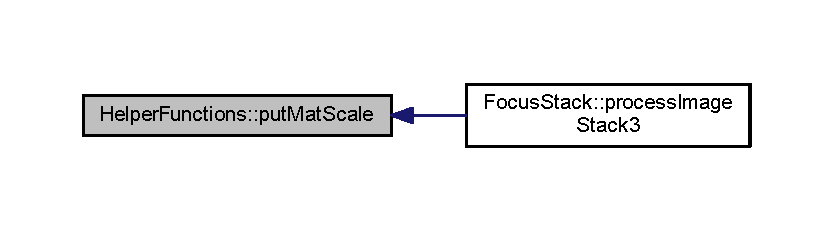
\includegraphics[width=350pt]{class_helper_functions_ad960d64773884aa54332b6b72ab5b876_icgraph}
\end{center}
\end{figure}
\mbox{\Hypertarget{class_helper_functions_af83ef83dc647e660335bf5564f5fdda7}\label{class_helper_functions_af83ef83dc647e660335bf5564f5fdda7}} 
\index{Helper\+Functions@{Helper\+Functions}!reflect@{reflect}}
\index{reflect@{reflect}!Helper\+Functions@{Helper\+Functions}}
\subsubsection{\texorpdfstring{reflect()}{reflect()}}
{\footnotesize\ttfamily int Helper\+Functions\+::reflect (\begin{DoxyParamCaption}\item[{int}]{M,  }\item[{int}]{x }\end{DoxyParamCaption})\hspace{0.3cm}{\ttfamily [static]}}

Handles vector boundaries by reflecting values

\begin{DoxyAuthor}{Author}
David Watts 
\end{DoxyAuthor}
\begin{DoxySince}{Since}
2017/03/07
\end{DoxySince}
Full\+Name \hyperlink{class_helper_functions_af83ef83dc647e660335bf5564f5fdda7}{Helper\+Functions\+::reflect} Qualifier 
\begin{DoxyParams}{Parameters}
{\em int} & M \\
\hline
{\em int} & x \\
\hline
\end{DoxyParams}
\begin{DoxyReturn}{Returns}
int Access public 
\end{DoxyReturn}


Definition at line 271 of file Helper\+Functions.\+cpp.

Here is the caller graph for this function\+:
\nopagebreak
\begin{figure}[H]
\begin{center}
\leavevmode
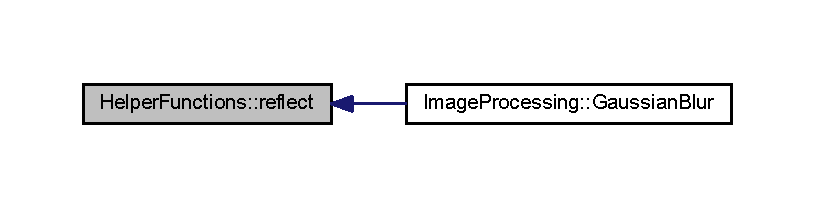
\includegraphics[width=350pt]{class_helper_functions_af83ef83dc647e660335bf5564f5fdda7_icgraph}
\end{center}
\end{figure}
\mbox{\Hypertarget{class_helper_functions_a7807daf795fa0056e924f191be8abaf9}\label{class_helper_functions_a7807daf795fa0056e924f191be8abaf9}} 
\index{Helper\+Functions@{Helper\+Functions}!rescale@{rescale}}
\index{rescale@{rescale}!Helper\+Functions@{Helper\+Functions}}
\subsubsection{\texorpdfstring{rescale()}{rescale()}}
{\footnotesize\ttfamily template$<$typename T $>$ \\
static void Helper\+Functions\+::rescale (\begin{DoxyParamCaption}\item[{T $\ast$}]{im,  }\item[{int}]{w,  }\item[{int}]{h }\end{DoxyParamCaption})\hspace{0.3cm}{\ttfamily [inline]}, {\ttfamily [static]}}

rescales image pixel values

\begin{DoxyAuthor}{Author}
David Watts 
\end{DoxyAuthor}
\begin{DoxySince}{Since}
2017/03/07
\end{DoxySince}
Full\+Name \hyperlink{class_helper_functions_a7807daf795fa0056e924f191be8abaf9}{Helper\+Functions\+::rescale} Qualifier 
\begin{DoxyParams}{Parameters}
{\em T} & $\ast$ im \\
\hline
{\em int} & w \\
\hline
{\em int} & h \\
\hline
\end{DoxyParams}
\begin{DoxyReturn}{Returns}
void Access public 
\end{DoxyReturn}


Definition at line 182 of file Helper\+Functions.\+h.

\mbox{\Hypertarget{class_helper_functions_a7afac4bb91186ab522a3a1d640589e7e}\label{class_helper_functions_a7afac4bb91186ab522a3a1d640589e7e}} 
\index{Helper\+Functions@{Helper\+Functions}!resize\+Image\+Preserve@{resize\+Image\+Preserve}}
\index{resize\+Image\+Preserve@{resize\+Image\+Preserve}!Helper\+Functions@{Helper\+Functions}}
\subsubsection{\texorpdfstring{resize\+Image\+Preserve()}{resizeImagePreserve()}}
{\footnotesize\ttfamily void Helper\+Functions\+::resize\+Image\+Preserve (\begin{DoxyParamCaption}\item[{cv\+::\+Mat \&}]{image\+In,  }\item[{cv\+::\+Mat \&}]{image\+Out,  }\item[{int}]{new\+Width,  }\item[{int}]{new\+Height }\end{DoxyParamCaption})\hspace{0.3cm}{\ttfamily [static]}}

Resizes image while preserving aspect ratio

\begin{DoxyAuthor}{Author}
David Watts 
\end{DoxyAuthor}
\begin{DoxySince}{Since}
2017/03/07
\end{DoxySince}
Full\+Name \hyperlink{class_helper_functions_a7afac4bb91186ab522a3a1d640589e7e}{Helper\+Functions\+::resize\+Image\+Preserve} Qualifier 
\begin{DoxyParams}{Parameters}
{\em cv\+::\+Mat} & \& image\+In \\
\hline
{\em cv\+::\+Mat} & \& image\+Out \\
\hline
{\em int} & new\+Width \\
\hline
{\em int} & new\+Height \\
\hline
\end{DoxyParams}
\begin{DoxyReturn}{Returns}
void Access public 
\end{DoxyReturn}


Definition at line 151 of file Helper\+Functions.\+cpp.

\mbox{\Hypertarget{class_helper_functions_a0b9d882eaf6b7d85aad907ee3e94d197}\label{class_helper_functions_a0b9d882eaf6b7d85aad907ee3e94d197}} 
\index{Helper\+Functions@{Helper\+Functions}!type2str@{type2str}}
\index{type2str@{type2str}!Helper\+Functions@{Helper\+Functions}}
\subsubsection{\texorpdfstring{type2str()}{type2str()}}
{\footnotesize\ttfamily string Helper\+Functions\+::type2str (\begin{DoxyParamCaption}\item[{int}]{type }\end{DoxyParamCaption})\hspace{0.3cm}{\ttfamily [static]}}

Returns a string representation of the opencv image type

\begin{DoxyAuthor}{Author}
David Watts 
\end{DoxyAuthor}
\begin{DoxySince}{Since}
2017/03/07
\end{DoxySince}
Full\+Name \hyperlink{class_helper_functions_a0b9d882eaf6b7d85aad907ee3e94d197}{Helper\+Functions\+::type2str} Qualifier 
\begin{DoxyParams}{Parameters}
{\em int} & type \\
\hline
\end{DoxyParams}
\begin{DoxyReturn}{Returns}
std\+::string Access public 
\end{DoxyReturn}


Definition at line 31 of file Helper\+Functions.\+cpp.

Here is the caller graph for this function\+:
\nopagebreak
\begin{figure}[H]
\begin{center}
\leavevmode
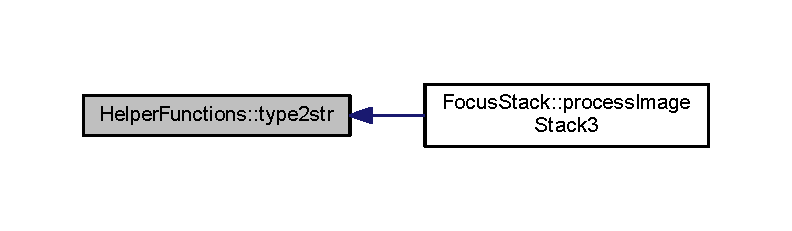
\includegraphics[width=350pt]{class_helper_functions_a0b9d882eaf6b7d85aad907ee3e94d197_icgraph}
\end{center}
\end{figure}


The documentation for this class was generated from the following files\+:\begin{DoxyCompactItemize}
\item 
H\+:/\+Code\+Projects/\+Q\+T\+Projects/\+Targeter-\/msvc/Helper\+Functions.\+h\item 
H\+:/\+Code\+Projects/\+Q\+T\+Projects/\+Targeter-\/msvc/Helper\+Functions.\+cpp\end{DoxyCompactItemize}

\hypertarget{structhist_cluster}{}\section{hist\+Cluster Struct Reference}
\label{structhist_cluster}\index{hist\+Cluster@{hist\+Cluster}}


{\ttfamily \#include $<$globals.\+h$>$}



Collaboration diagram for hist\+Cluster\+:
\nopagebreak
\begin{figure}[H]
\begin{center}
\leavevmode
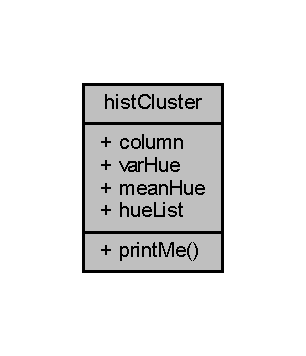
\includegraphics[width=147pt]{structhist_cluster__coll__graph}
\end{center}
\end{figure}
\subsection*{Public Member Functions}
\begin{DoxyCompactItemize}
\item 
\mbox{\Hypertarget{structhist_cluster_ad101156d19fc78ca6e33e3c08e98bb39}\label{structhist_cluster_ad101156d19fc78ca6e33e3c08e98bb39}} 
void {\bfseries print\+Me} (std\+::string s=\char`\"{}\char`\"{})
\end{DoxyCompactItemize}
\subsection*{Public Attributes}
\begin{DoxyCompactItemize}
\item 
\mbox{\Hypertarget{structhist_cluster_af783140907cf13bc6bdfabfecd70311b}\label{structhist_cluster_af783140907cf13bc6bdfabfecd70311b}} 
std\+::vector$<$ \hyperlink{structhistogram_bar}{histogram\+Bar} $>$ {\bfseries column}
\item 
\mbox{\Hypertarget{structhist_cluster_a9eda24704dde33b207b2fd5682b505ee}\label{structhist_cluster_a9eda24704dde33b207b2fd5682b505ee}} 
float \hyperlink{structhist_cluster_a9eda24704dde33b207b2fd5682b505ee}{var\+Hue}
\begin{DoxyCompactList}\small\item\em each histogram column as vector \end{DoxyCompactList}\item 
\mbox{\Hypertarget{structhist_cluster_af92ce9628948aec76afa20f7776caff2}\label{structhist_cluster_af92ce9628948aec76afa20f7776caff2}} 
float \hyperlink{structhist_cluster_af92ce9628948aec76afa20f7776caff2}{mean\+Hue}
\begin{DoxyCompactList}\small\item\em variance \end{DoxyCompactList}\item 
\mbox{\Hypertarget{structhist_cluster_a21a6b3ad886acdf8ab396ac5ec87875b}\label{structhist_cluster_a21a6b3ad886acdf8ab396ac5ec87875b}} 
std\+::vector$<$ int $>$ \hyperlink{structhist_cluster_a21a6b3ad886acdf8ab396ac5ec87875b}{hue\+List}
\begin{DoxyCompactList}\small\item\em mean \end{DoxyCompactList}\end{DoxyCompactItemize}


\subsection{Detailed Description}
structure to represent vector of histogram bars, ie. whole histogram 

Definition at line 172 of file globals.\+h.



The documentation for this struct was generated from the following file\+:\begin{DoxyCompactItemize}
\item 
H\+:/\+Code\+Projects/\+Q\+T\+Projects/\+Targeter-\/msvc/globals.\+h\end{DoxyCompactItemize}

\hypertarget{structhistogram_bar}{}\section{histogram\+Bar Struct Reference}
\label{structhistogram_bar}\index{histogram\+Bar@{histogram\+Bar}}


{\ttfamily \#include $<$globals.\+h$>$}



Collaboration diagram for histogram\+Bar\+:
\nopagebreak
\begin{figure}[H]
\begin{center}
\leavevmode
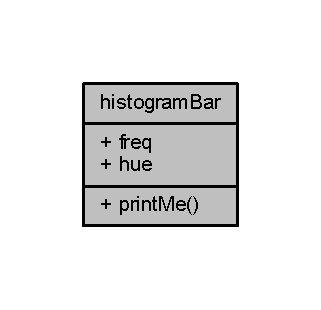
\includegraphics[width=154pt]{structhistogram_bar__coll__graph}
\end{center}
\end{figure}
\subsection*{Public Member Functions}
\begin{DoxyCompactItemize}
\item 
\mbox{\Hypertarget{structhistogram_bar_a8202ebe23bca4d5f765a9af5947f6a3c}\label{structhistogram_bar_a8202ebe23bca4d5f765a9af5947f6a3c}} 
void \hyperlink{structhistogram_bar_a8202ebe23bca4d5f765a9af5947f6a3c}{print\+Me} (std\+::string s=\char`\"{}\char`\"{})
\begin{DoxyCompactList}\small\item\em position of histogram (hue or grayscale) \end{DoxyCompactList}\end{DoxyCompactItemize}
\subsection*{Public Attributes}
\begin{DoxyCompactItemize}
\item 
\mbox{\Hypertarget{structhistogram_bar_aabef82c0a6adc7d9e999f4da203cf97c}\label{structhistogram_bar_aabef82c0a6adc7d9e999f4da203cf97c}} 
float {\bfseries freq}
\item 
\mbox{\Hypertarget{structhistogram_bar_a39a1bed319d0844a832dc30852caaeda}\label{structhistogram_bar_a39a1bed319d0844a832dc30852caaeda}} 
double \hyperlink{structhistogram_bar_a39a1bed319d0844a832dc30852caaeda}{hue}
\begin{DoxyCompactList}\small\item\em count of histogram (normalised) \end{DoxyCompactList}\end{DoxyCompactItemize}


\subsection{Detailed Description}
structure to represent histogram bar 

Definition at line 159 of file globals.\+h.



The documentation for this struct was generated from the following file\+:\begin{DoxyCompactItemize}
\item 
H\+:/\+Code\+Projects/\+Q\+T\+Projects/\+Targeter-\/msvc/globals.\+h\end{DoxyCompactItemize}

\hypertarget{class_image_processing}{}\section{Image\+Processing Class Reference}
\label{class_image_processing}\index{Image\+Processing@{Image\+Processing}}


{\ttfamily \#include $<$imageprocessing.\+h$>$}



Collaboration diagram for Image\+Processing\+:
\nopagebreak
\begin{figure}[H]
\begin{center}
\leavevmode
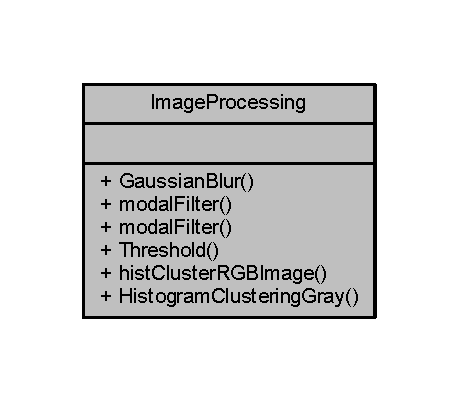
\includegraphics[width=220pt]{class_image_processing__coll__graph}
\end{center}
\end{figure}
\subsection*{Static Public Member Functions}
\begin{DoxyCompactItemize}
\item 
static void \hyperlink{class_image_processing_a07eb3c4d3eb55ea7bb8dd9e57190bb3a}{Gaussian\+Blur} (int $\ast$im, int w, int h, int repeat)
\item 
static void \hyperlink{class_image_processing_ae1460831474adb16ed769cd6956ddbff}{modal\+Filter} (int $\ast$im, int w, int h, int f\+Size, int No\+Focus\+Images)
\item 
\mbox{\Hypertarget{class_image_processing_a67b372b99a529c42c825623f49f58d4d}\label{class_image_processing_a67b372b99a529c42c825623f49f58d4d}} 
static void {\bfseries modal\+Filter} (cv\+::\+Mat \&im, int w, int h, int f\+Size, int No\+Focus\+Images)
\item 
static cv\+::\+Mat \hyperlink{class_image_processing_ae664598cc3952b81d2bbe59dfd0f0d94}{Threshold} (cv\+::\+Mat \&im, int min, int max)
\item 
static int $\ast$ \hyperlink{class_image_processing_ad95299703a3db5104a65c162dd07d5f9}{hist\+Cluster\+R\+G\+B\+Image} (cv\+::\+Mat hue\+Hist, int hist\+Size, int No\+Cluster=2)
\item 
static cv\+::\+Mat \hyperlink{class_image_processing_a4f0e35a8e54832a3d447c6fbeba5f11a}{Histogram\+Clustering\+Gray} (cv\+::\+Mat im, int No\+Clusters=2)
\end{DoxyCompactItemize}


\subsection{Detailed Description}
class to for image processing functionality shared by other classes 

Definition at line 11 of file imageprocessing.\+h.



\subsection{Member Function Documentation}
\mbox{\Hypertarget{class_image_processing_a07eb3c4d3eb55ea7bb8dd9e57190bb3a}\label{class_image_processing_a07eb3c4d3eb55ea7bb8dd9e57190bb3a}} 
\index{Image\+Processing@{Image\+Processing}!Gaussian\+Blur@{Gaussian\+Blur}}
\index{Gaussian\+Blur@{Gaussian\+Blur}!Image\+Processing@{Image\+Processing}}
\subsubsection{\texorpdfstring{Gaussian\+Blur()}{GaussianBlur()}}
{\footnotesize\ttfamily void Image\+Processing\+::\+Gaussian\+Blur (\begin{DoxyParamCaption}\item[{int $\ast$}]{im,  }\item[{int}]{w,  }\item[{int}]{h,  }\item[{int}]{repeat }\end{DoxyParamCaption})\hspace{0.3cm}{\ttfamily [static]}}

Performs Guassian blur filter on 1D int$\ast$ image

\begin{DoxyAuthor}{Author}
David Watts 
\end{DoxyAuthor}
\begin{DoxySince}{Since}
2017/03/07
\end{DoxySince}
Full\+Name \hyperlink{class_image_processing_a07eb3c4d3eb55ea7bb8dd9e57190bb3a}{Image\+Processing\+::\+Gaussian\+Blur} Qualifier 
\begin{DoxyParams}{Parameters}
{\em int} & $\ast$ im \\
\hline
{\em int} & w \\
\hline
{\em int} & h \\
\hline
{\em int} & repeat \\
\hline
\end{DoxyParams}
\begin{DoxyReturn}{Returns}
void Access public 
\end{DoxyReturn}


Definition at line 504 of file imageprocessing.\+cpp.

Here is the call graph for this function\+:
\nopagebreak
\begin{figure}[H]
\begin{center}
\leavevmode
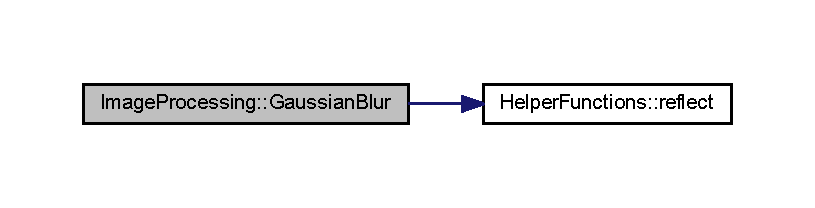
\includegraphics[width=350pt]{class_image_processing_a07eb3c4d3eb55ea7bb8dd9e57190bb3a_cgraph}
\end{center}
\end{figure}
\mbox{\Hypertarget{class_image_processing_ad95299703a3db5104a65c162dd07d5f9}\label{class_image_processing_ad95299703a3db5104a65c162dd07d5f9}} 
\index{Image\+Processing@{Image\+Processing}!hist\+Cluster\+R\+G\+B\+Image@{hist\+Cluster\+R\+G\+B\+Image}}
\index{hist\+Cluster\+R\+G\+B\+Image@{hist\+Cluster\+R\+G\+B\+Image}!Image\+Processing@{Image\+Processing}}
\subsubsection{\texorpdfstring{hist\+Cluster\+R\+G\+B\+Image()}{histClusterRGBImage()}}
{\footnotesize\ttfamily int $\ast$ Image\+Processing\+::hist\+Cluster\+R\+G\+B\+Image (\begin{DoxyParamCaption}\item[{cv\+::\+Mat}]{hue\+Hist,  }\item[{int}]{hist\+Size,  }\item[{int}]{No\+Clusters = {\ttfamily 2} }\end{DoxyParamCaption})\hspace{0.3cm}{\ttfamily [static]}}

Returns image that has been posterized based on method of histogram variances

\begin{DoxyAuthor}{Author}
David Watts 
\end{DoxyAuthor}
\begin{DoxySince}{Since}
2017/03/07
\end{DoxySince}
Full\+Name \hyperlink{class_image_processing_ad95299703a3db5104a65c162dd07d5f9}{Image\+Processing\+::hist\+Cluster\+R\+G\+B\+Image} Qualifier 
\begin{DoxyParams}{Parameters}
{\em cv\+::\+Mat} & hue\+Hist \\
\hline
{\em int} & hist\+Size \\
\hline
{\em int} & No\+Clusters \\
\hline
\end{DoxyParams}
\begin{DoxyReturn}{Returns}
int$\ast$ Access public 
\end{DoxyReturn}


Definition at line 169 of file imageprocessing.\+cpp.

Here is the call graph for this function\+:
\nopagebreak
\begin{figure}[H]
\begin{center}
\leavevmode
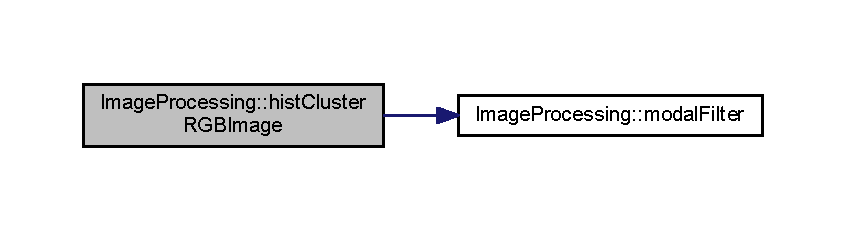
\includegraphics[width=350pt]{class_image_processing_ad95299703a3db5104a65c162dd07d5f9_cgraph}
\end{center}
\end{figure}
\mbox{\Hypertarget{class_image_processing_a4f0e35a8e54832a3d447c6fbeba5f11a}\label{class_image_processing_a4f0e35a8e54832a3d447c6fbeba5f11a}} 
\index{Image\+Processing@{Image\+Processing}!Histogram\+Clustering\+Gray@{Histogram\+Clustering\+Gray}}
\index{Histogram\+Clustering\+Gray@{Histogram\+Clustering\+Gray}!Image\+Processing@{Image\+Processing}}
\subsubsection{\texorpdfstring{Histogram\+Clustering\+Gray()}{HistogramClusteringGray()}}
{\footnotesize\ttfamily cv\+::\+Mat Image\+Processing\+::\+Histogram\+Clustering\+Gray (\begin{DoxyParamCaption}\item[{cv\+::\+Mat}]{im,  }\item[{int}]{No\+Clusters = {\ttfamily 2} }\end{DoxyParamCaption})\hspace{0.3cm}{\ttfamily [static]}}

Returns posterized opencv image which has No\+Clusters numbers of levels

\begin{DoxyAuthor}{Author}
David Watts 
\end{DoxyAuthor}
\begin{DoxySince}{Since}
2017/03/07
\end{DoxySince}
Full\+Name \hyperlink{class_image_processing_a4f0e35a8e54832a3d447c6fbeba5f11a}{Image\+Processing\+::\+Histogram\+Clustering\+Gray} Qualifier 
\begin{DoxyParams}{Parameters}
{\em cv\+::\+Mat} & im \\
\hline
{\em int} & No\+Clusters \\
\hline
\end{DoxyParams}
\begin{DoxyReturn}{Returns}
cv\+::\+Mat Access public 
\end{DoxyReturn}


Definition at line 80 of file imageprocessing.\+cpp.

Here is the caller graph for this function\+:
\nopagebreak
\begin{figure}[H]
\begin{center}
\leavevmode
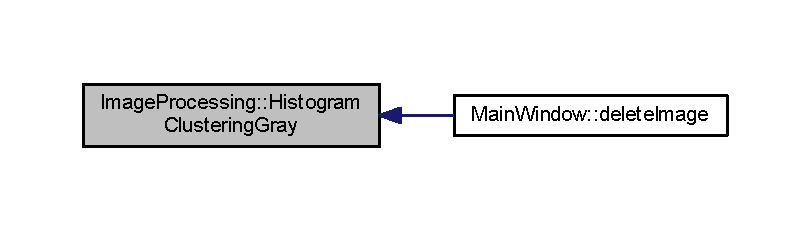
\includegraphics[width=350pt]{class_image_processing_a4f0e35a8e54832a3d447c6fbeba5f11a_icgraph}
\end{center}
\end{figure}
\mbox{\Hypertarget{class_image_processing_ae1460831474adb16ed769cd6956ddbff}\label{class_image_processing_ae1460831474adb16ed769cd6956ddbff}} 
\index{Image\+Processing@{Image\+Processing}!modal\+Filter@{modal\+Filter}}
\index{modal\+Filter@{modal\+Filter}!Image\+Processing@{Image\+Processing}}
\subsubsection{\texorpdfstring{modal\+Filter()}{modalFilter()}}
{\footnotesize\ttfamily void Image\+Processing\+::modal\+Filter (\begin{DoxyParamCaption}\item[{int $\ast$}]{im,  }\item[{int}]{w,  }\item[{int}]{h,  }\item[{int}]{f\+Size,  }\item[{int}]{No\+Focus\+Images }\end{DoxyParamCaption})\hspace{0.3cm}{\ttfamily [static]}}

performs modal filter on 1D int$\ast$ image

\begin{DoxyAuthor}{Author}
David Watts 
\end{DoxyAuthor}
\begin{DoxySince}{Since}
2017/03/07
\end{DoxySince}
Full\+Name \hyperlink{class_image_processing_ae1460831474adb16ed769cd6956ddbff}{Image\+Processing\+::modal\+Filter} Qualifier 
\begin{DoxyParams}{Parameters}
{\em int} & $\ast$ im \\
\hline
{\em int} & w \\
\hline
{\em int} & h \\
\hline
{\em int} & f\+Size \\
\hline
{\em int} & No\+Focus\+Images \\
\hline
\end{DoxyParams}
\begin{DoxyReturn}{Returns}
void Access public 
\end{DoxyReturn}


Definition at line 431 of file imageprocessing.\+cpp.

Here is the caller graph for this function\+:
\nopagebreak
\begin{figure}[H]
\begin{center}
\leavevmode
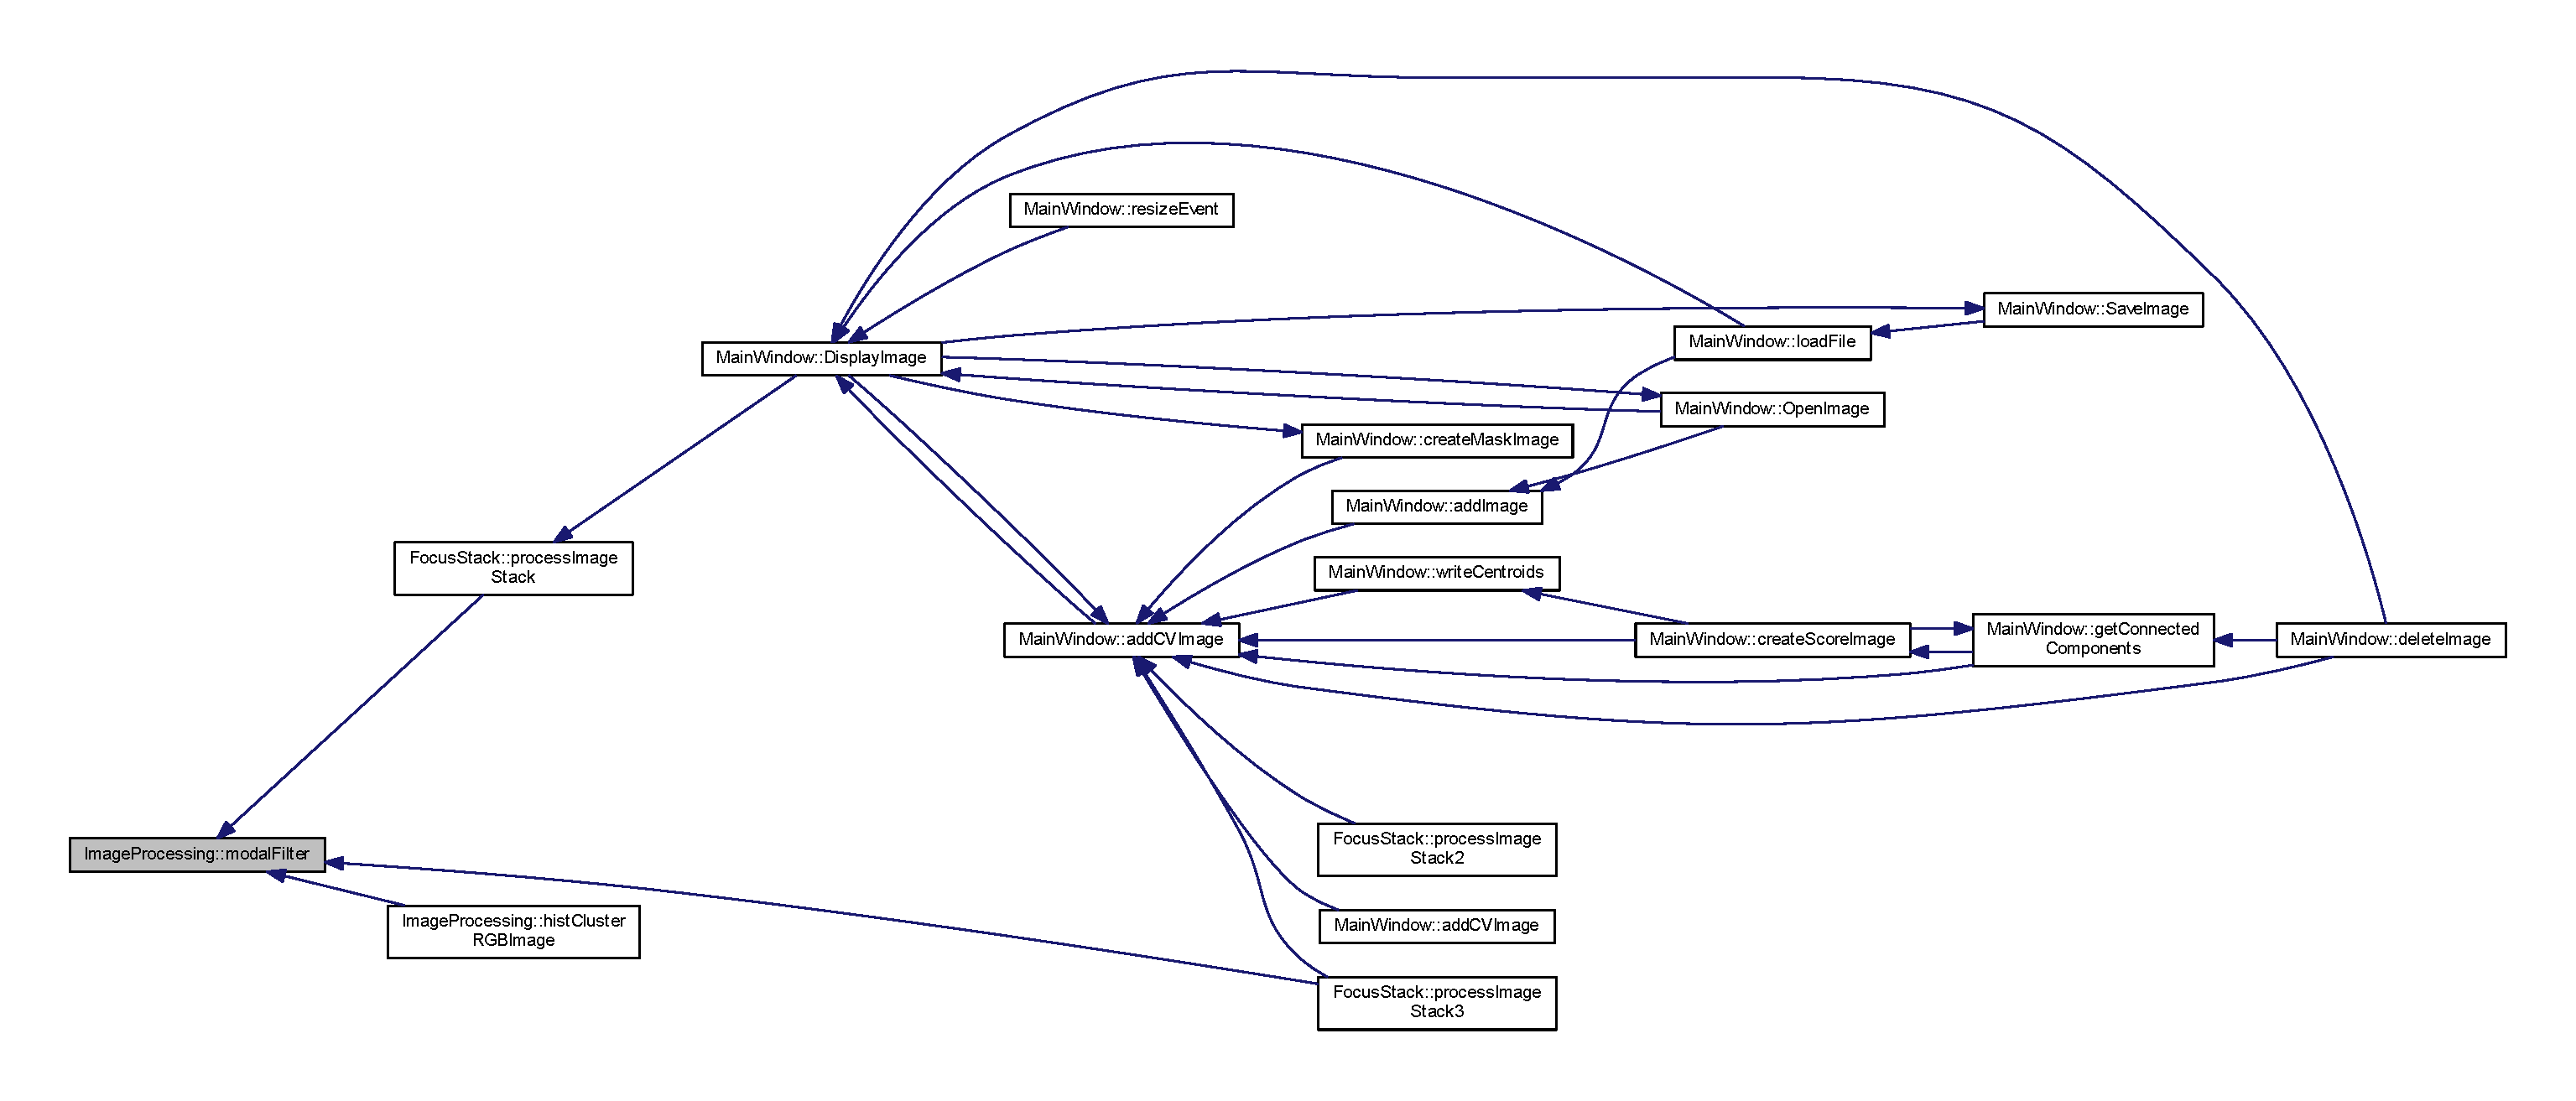
\includegraphics[width=350pt]{class_image_processing_ae1460831474adb16ed769cd6956ddbff_icgraph}
\end{center}
\end{figure}
\mbox{\Hypertarget{class_image_processing_ae664598cc3952b81d2bbe59dfd0f0d94}\label{class_image_processing_ae664598cc3952b81d2bbe59dfd0f0d94}} 
\index{Image\+Processing@{Image\+Processing}!Threshold@{Threshold}}
\index{Threshold@{Threshold}!Image\+Processing@{Image\+Processing}}
\subsubsection{\texorpdfstring{Threshold()}{Threshold()}}
{\footnotesize\ttfamily cv\+::\+Mat Image\+Processing\+::\+Threshold (\begin{DoxyParamCaption}\item[{cv\+::\+Mat \&}]{im,  }\item[{int}]{min,  }\item[{int}]{max }\end{DoxyParamCaption})\hspace{0.3cm}{\ttfamily [static]}}

Threshold image between min and max greyscale values

\begin{DoxyAuthor}{Author}
David Watts 
\end{DoxyAuthor}
\begin{DoxySince}{Since}
2017/03/07
\end{DoxySince}
Full\+Name \hyperlink{class_image_processing_ae664598cc3952b81d2bbe59dfd0f0d94}{Image\+Processing\+::\+Threshold} Qualifier 
\begin{DoxyParams}{Parameters}
{\em Mat} & \& im \\
\hline
{\em int} & min \\
\hline
{\em int} & max \\
\hline
\end{DoxyParams}
\begin{DoxyReturn}{Returns}
cv\+::\+Mat Access public 
\end{DoxyReturn}


Definition at line 32 of file imageprocessing.\+cpp.

Here is the caller graph for this function\+:
\nopagebreak
\begin{figure}[H]
\begin{center}
\leavevmode
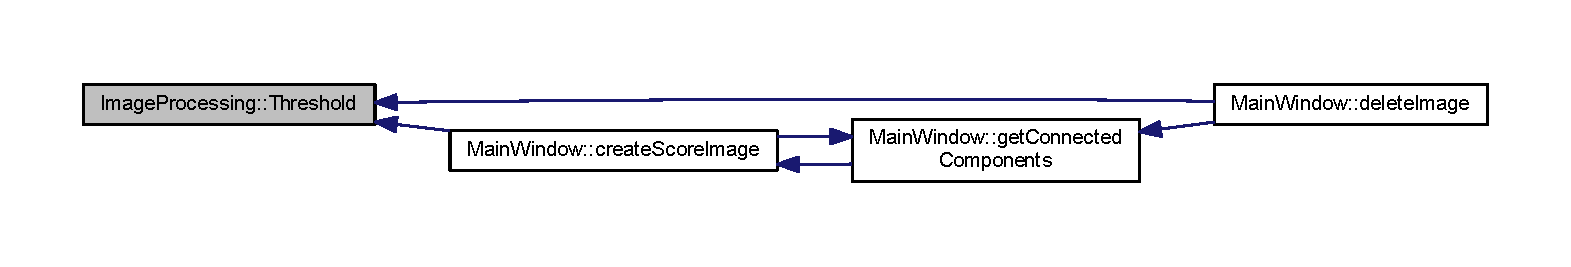
\includegraphics[width=350pt]{class_image_processing_ae664598cc3952b81d2bbe59dfd0f0d94_icgraph}
\end{center}
\end{figure}


The documentation for this class was generated from the following files\+:\begin{DoxyCompactItemize}
\item 
H\+:/\+Code\+Projects/\+Q\+T\+Projects/\+Targeter-\/msvc/imageprocessing.\+h\item 
H\+:/\+Code\+Projects/\+Q\+T\+Projects/\+Targeter-\/msvc/imageprocessing.\+cpp\end{DoxyCompactItemize}

\hypertarget{class_images_container}{}\section{Images\+Container Class Reference}
\label{class_images_container}\index{Images\+Container@{Images\+Container}}


{\ttfamily \#include $<$images\+Container.\+h$>$}



Collaboration diagram for Images\+Container\+:
\nopagebreak
\begin{figure}[H]
\begin{center}
\leavevmode
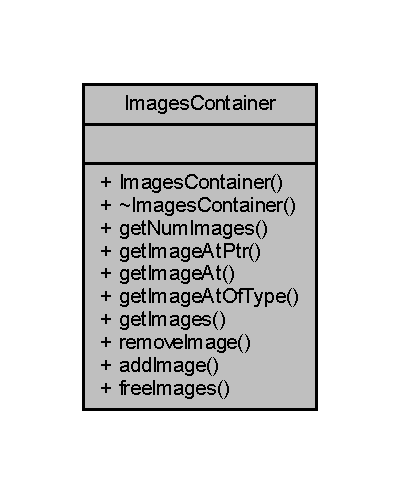
\includegraphics[width=192pt]{class_images_container__coll__graph}
\end{center}
\end{figure}
\subsection*{Public Member Functions}
\begin{DoxyCompactItemize}
\item 
\mbox{\Hypertarget{class_images_container_a0b318e09e4bef3654167c753173062db}\label{class_images_container_a0b318e09e4bef3654167c753173062db}} 
int {\bfseries get\+Num\+Images} ()
\item 
\mbox{\Hypertarget{class_images_container_abfb496674a35192bb3911ef5de704e5d}\label{class_images_container_abfb496674a35192bb3911ef5de704e5d}} 
\hyperlink{classtargeter_image}{targeter\+Image} $\ast$ {\bfseries get\+Image\+At\+Ptr} (int i)
\item 
\mbox{\Hypertarget{class_images_container_abd99550c899f54291d9a449287bf89cc}\label{class_images_container_abd99550c899f54291d9a449287bf89cc}} 
\hyperlink{classtargeter_image}{targeter\+Image} \& {\bfseries get\+Image\+At} (int i)
\item 
\mbox{\Hypertarget{class_images_container_a6c7aea31ee7e6ec8c4c29f677ae57102}\label{class_images_container_a6c7aea31ee7e6ec8c4c29f677ae57102}} 
\hyperlink{classtargeter_image}{targeter\+Image} $\ast$ {\bfseries get\+Image\+At\+Of\+Type} (int i, image\+Type\+::image\+Type type)
\item 
\mbox{\Hypertarget{class_images_container_a3a7d1fe60da597aa0bd1eb5e7d95a5b7}\label{class_images_container_a3a7d1fe60da597aa0bd1eb5e7d95a5b7}} 
std\+::vector$<$ \hyperlink{classtargeter_image}{targeter\+Image} $>$ {\bfseries get\+Images} ()
\item 
\mbox{\Hypertarget{class_images_container_a7d26fc141f4a3f0b01530b232cc4ba3d}\label{class_images_container_a7d26fc141f4a3f0b01530b232cc4ba3d}} 
void {\bfseries remove\+Image} (int ind)
\item 
\mbox{\Hypertarget{class_images_container_af2acb74349b643c59e4d1e23ec17ab2e}\label{class_images_container_af2acb74349b643c59e4d1e23ec17ab2e}} 
void {\bfseries add\+Image} (\hyperlink{classtargeter_image}{targeter\+Image} \&im)
\item 
\mbox{\Hypertarget{class_images_container_aaa184b4198472cd81a8dfeb242644369}\label{class_images_container_aaa184b4198472cd81a8dfeb242644369}} 
void {\bfseries free\+Images} ()
\end{DoxyCompactItemize}


\subsection{Detailed Description}
class to store all images 

Definition at line 9 of file images\+Container.\+h.



The documentation for this class was generated from the following file\+:\begin{DoxyCompactItemize}
\item 
H\+:/\+Code\+Projects/\+Q\+T\+Projects/\+Targeter-\/msvc/images\+Container.\+h\end{DoxyCompactItemize}

\hypertarget{class_main_window}{}\section{Main\+Window Class Reference}
\label{class_main_window}\index{Main\+Window@{Main\+Window}}


{\ttfamily \#include $<$mainwindow.\+h$>$}



Inheritance diagram for Main\+Window\+:
\nopagebreak
\begin{figure}[H]
\begin{center}
\leavevmode
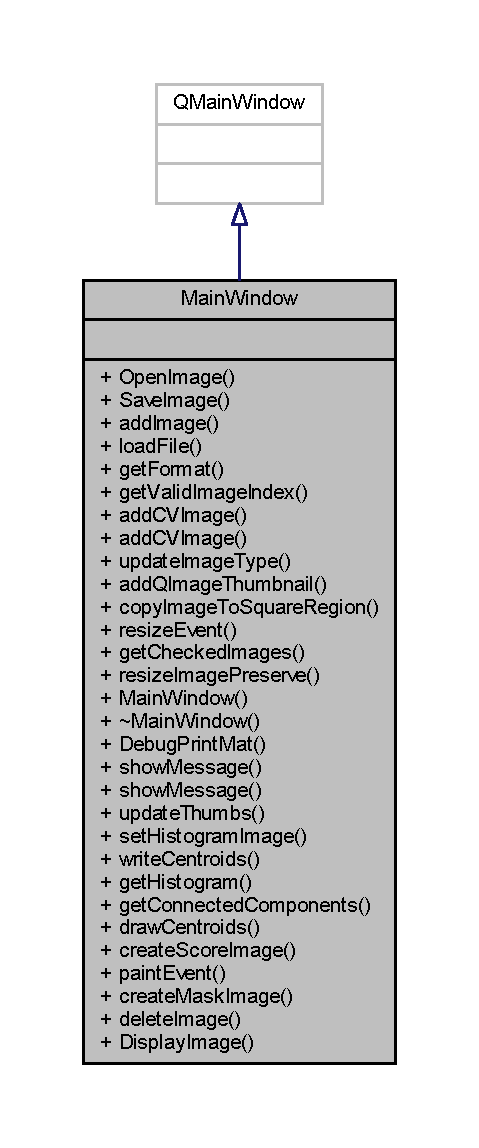
\includegraphics[height=550pt]{class_main_window__inherit__graph}
\end{center}
\end{figure}


Collaboration diagram for Main\+Window\+:
\nopagebreak
\begin{figure}[H]
\begin{center}
\leavevmode
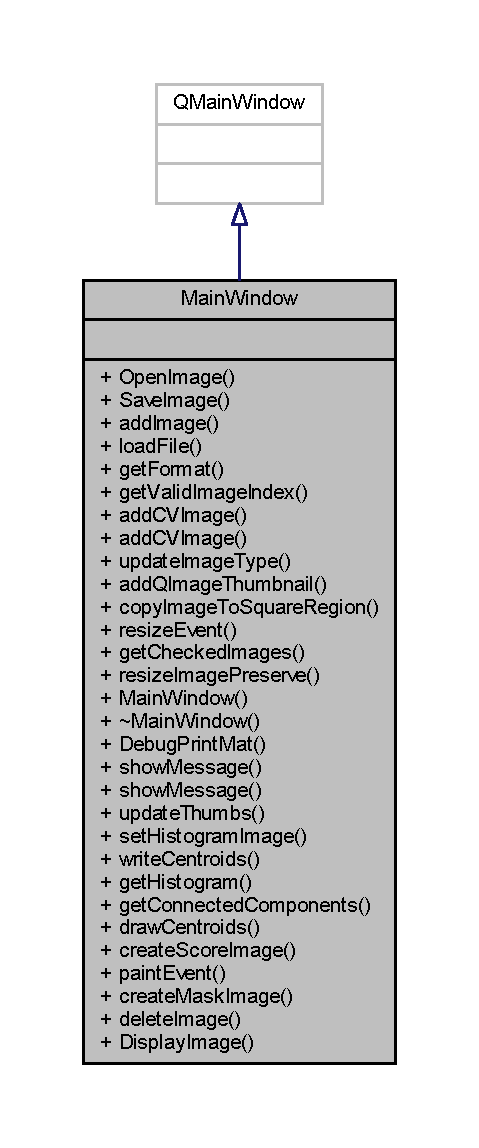
\includegraphics[height=550pt]{class_main_window__coll__graph}
\end{center}
\end{figure}
\subsection*{Public Slots}
\begin{DoxyCompactItemize}
\item 
void \hyperlink{class_main_window_a8e20e1254b179ca9ec054ec908d9cc43}{Display\+Image} ()
\end{DoxyCompactItemize}
\subsection*{Public Member Functions}
\begin{DoxyCompactItemize}
\item 
void \hyperlink{class_main_window_acea9cebdcf70bf45107baa0789e732bf}{Open\+Image} ()
\item 
void \hyperlink{class_main_window_aa816921e6ce14f558ada5c73c8a5ef20}{Save\+Image} ()
\item 
void \hyperlink{class_main_window_ab4d1f49d192d3641e0da68b5a69d014a}{add\+Image} (const Q\+String \&file\+Name, image\+Type\+::image\+Type type=image\+Type\+::display)
\item 
void \hyperlink{class_main_window_aa08469ed5c8396e60fa44bae6530bcf1}{load\+File} (const Q\+String \&file\+Name)
\item 
\mbox{\Hypertarget{class_main_window_a15007754f8c9ca7ab8e2886fd321d33d}\label{class_main_window_a15007754f8c9ca7ab8e2886fd321d33d}} 
Q\+Image\+::\+Format {\bfseries get\+Format} (int type)
\item 
int \hyperlink{class_main_window_acc35ff9a0c04d62297e7fd219fa869e5}{get\+Valid\+Image\+Index} ()
\item 
void \hyperlink{class_main_window_a0c29749703b7fc8a64a17d123816bfac}{add\+C\+V\+Image} (\hyperlink{classtargeter_image}{targeter\+Image} \&tim, Q\+String image\+Name, bool b\+R\+G\+B\+Swap)
\item 
void \hyperlink{class_main_window_ab87edc0e4b2fb3e4fb4df14a8872cbb4}{add\+C\+V\+Image} (cv\+::\+Mat im, Q\+String image\+Name=\char`\"{}\char`\"{}, bool b\+R\+G\+B\+Swap=true, image\+Type\+::image\+Type type=image\+Type\+::display, bool b\+Display=true)
\item 
void \hyperlink{class_main_window_a171b0591a4f66b4b16a33d4af5c35465}{update\+Image\+Type} (int ind, image\+Type\+::image\+Type type)
\item 
void \hyperlink{class_main_window_a8b60c57f82b0ac86df7c64692294a35e}{add\+Q\+Image\+Thumbnail} (Q\+Image \&qim, Q\+String image\+Name=\char`\"{}\char`\"{}, image\+Type\+::image\+Type type=image\+Type\+::display)
\item 
Q\+Image \hyperlink{class_main_window_a5e034c81127e2a14248eb81414e1e96e}{copy\+Image\+To\+Square\+Region} (Q\+Image im, Q\+Color col)
\item 
void \hyperlink{class_main_window_ae12f8f63791595567b6250f8bb002bda}{resize\+Event} (Q\+Resize\+Event $\ast$event)
\item 
std\+::vector$<$ int $>$ \hyperlink{class_main_window_a1e798fdae21c3294495ea7994df1887a}{get\+Checked\+Images} ()
\item 
\mbox{\Hypertarget{class_main_window_a2b4203abdf454313ed5bf11d38ae70f5}\label{class_main_window_a2b4203abdf454313ed5bf11d38ae70f5}} 
void {\bfseries resize\+Image\+Preserve} (cv\+::\+Mat \&in, cv\+::\+Mat \&out, int new\+Width, int new\+Height)
\item 
\hyperlink{class_main_window_a8b244be8b7b7db1b08de2a2acb9409db}{Main\+Window} (Q\+Widget $\ast$parent=0)
\item 
\hyperlink{class_main_window_ae98d00a93bc118200eeef9f9bba1dba7}{$\sim$\+Main\+Window} ()
\item 
\mbox{\Hypertarget{class_main_window_a838a9764a5001c205b964fd5e89742d2}\label{class_main_window_a838a9764a5001c205b964fd5e89742d2}} 
void {\bfseries Debug\+Print\+Mat} (cv\+::\+Mat mat)
\item 
void \hyperlink{class_main_window_a280d25148ac076ca817d411372584ae5}{show\+Message} (image\+Type\+::image\+Type, Q\+Message\+Box\+::\+Icon icn=Q\+Message\+Box\+::\+Warning)
\item 
void \hyperlink{class_main_window_aebde68c58d77b71d20fa6816b751356e}{show\+Message} (Q\+String message, Q\+Message\+Box\+::\+Icon icn=Q\+Message\+Box\+::\+Warning)
\item 
void \hyperlink{class_main_window_a89dfa31ef44692bb1d7307f0c35838c0}{update\+Thumbs} (int index=-\/1)
\item 
void \hyperlink{class_main_window_a5e130e8122dbab96f931a7ecc41086d3}{set\+Histogram\+Image} ()
\item 
void \hyperlink{class_main_window_aa137f4371bae807873da7862f4102521}{write\+Centroids} (\hyperlink{classtargeter_image}{targeter\+Image} \&tim, Q\+File \&xml\+File)
\item 
cv\+::\+Mat \hyperlink{class_main_window_a2734ce9308b5847a561f00b2fc9066aa}{get\+Histogram} ()
\item 
\hyperlink{classtargeter_image}{targeter\+Image} \hyperlink{class_main_window_a49cfabc6ef4845c5a9b5c9a92c9d4e2e}{get\+Connected\+Components} (cv\+::\+Mat \&im)
\item 
void \hyperlink{class_main_window_ad68b6789cc86ef20cd7cedd6de8d4ed2}{draw\+Centroids} (\hyperlink{classtargeter_image}{targeter\+Image} \&tim, cv\+::\+Mat \&drawimage)
\item 
cv\+::\+Mat \hyperlink{class_main_window_a8d87cd33d22ce614c9d7945264588e5f}{create\+Score\+Image} ()
\item 
\mbox{\Hypertarget{class_main_window_abf05d580e91f725777cdb6a5eb0bf08c}\label{class_main_window_abf05d580e91f725777cdb6a5eb0bf08c}} 
virtual void {\bfseries paint\+Event} (Q\+Paint\+Event $\ast$event)
\item 
void \hyperlink{class_main_window_a92a40847027eaf2cf258c3a9f8da4c48}{create\+Mask\+Image} (cv\+::\+Mat im, \hyperlink{structdrawing_shape}{drawing\+Shape} shape)
\item 
void \hyperlink{class_main_window_ad0219fc878a0bc02403d00a16b7fc7ec}{delete\+Image} (int index, bool b\+Display=true)
\end{DoxyCompactItemize}


\subsection{Detailed Description}
Main Q\+T\+Main\+Window derived class for managing window display 

Definition at line 25 of file mainwindow.\+h.



\subsection{Constructor \& Destructor Documentation}
\mbox{\Hypertarget{class_main_window_a8b244be8b7b7db1b08de2a2acb9409db}\label{class_main_window_a8b244be8b7b7db1b08de2a2acb9409db}} 
\index{Main\+Window@{Main\+Window}!Main\+Window@{Main\+Window}}
\index{Main\+Window@{Main\+Window}!Main\+Window@{Main\+Window}}
\subsubsection{\texorpdfstring{Main\+Window()}{MainWindow()}}
{\footnotesize\ttfamily Main\+Window\+::\+Main\+Window (\begin{DoxyParamCaption}\item[{Q\+Widget $\ast$}]{parent = {\ttfamily 0} }\end{DoxyParamCaption})\hspace{0.3cm}{\ttfamily [explicit]}}

class constructor\+: sets up slots, initializes variables, gets serialised settings values

\begin{DoxyAuthor}{Author}
David Watts 
\end{DoxyAuthor}
\begin{DoxySince}{Since}
2017/03/07
\end{DoxySince}
Full\+Name \hyperlink{class_main_window_a8b244be8b7b7db1b08de2a2acb9409db}{Main\+Window\+::\+Main\+Window} Qualifier \+: Q\+Main\+Window(parent), ui(new Ui\+::\+Main\+Window) 
\begin{DoxyParams}{Parameters}
{\em Q\+Widget} & $\ast$ parent \\
\hline
\end{DoxyParams}
\begin{DoxyReturn}{Returns}
Access public 
\end{DoxyReturn}


Definition at line 73 of file mainwindow.\+cpp.

Here is the call graph for this function\+:
\nopagebreak
\begin{figure}[H]
\begin{center}
\leavevmode
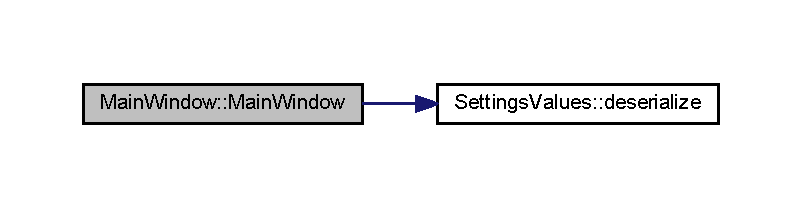
\includegraphics[width=350pt]{class_main_window_a8b244be8b7b7db1b08de2a2acb9409db_cgraph}
\end{center}
\end{figure}
\mbox{\Hypertarget{class_main_window_ae98d00a93bc118200eeef9f9bba1dba7}\label{class_main_window_ae98d00a93bc118200eeef9f9bba1dba7}} 
\index{Main\+Window@{Main\+Window}!````~Main\+Window@{$\sim$\+Main\+Window}}
\index{````~Main\+Window@{$\sim$\+Main\+Window}!Main\+Window@{Main\+Window}}
\subsubsection{\texorpdfstring{$\sim$\+Main\+Window()}{~MainWindow()}}
{\footnotesize\ttfamily Main\+Window\+::$\sim$\+Main\+Window (\begin{DoxyParamCaption}{ }\end{DoxyParamCaption})}

class destructor, serializes settings values

\begin{DoxyAuthor}{Author}
David Watts 
\end{DoxyAuthor}
\begin{DoxySince}{Since}
2017/03/07
\end{DoxySince}
Full\+Name \hyperlink{class_main_window_ae98d00a93bc118200eeef9f9bba1dba7}{Main\+Window\+::$\sim$\+Main\+Window} Qualifier \begin{DoxyReturn}{Returns}
Access public 
\end{DoxyReturn}


Definition at line 983 of file mainwindow.\+cpp.

Here is the call graph for this function\+:
\nopagebreak
\begin{figure}[H]
\begin{center}
\leavevmode
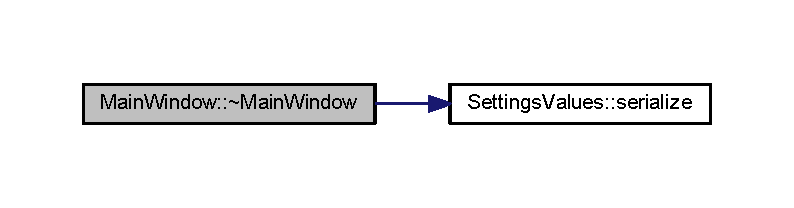
\includegraphics[width=350pt]{class_main_window_ae98d00a93bc118200eeef9f9bba1dba7_cgraph}
\end{center}
\end{figure}


\subsection{Member Function Documentation}
\mbox{\Hypertarget{class_main_window_a0c29749703b7fc8a64a17d123816bfac}\label{class_main_window_a0c29749703b7fc8a64a17d123816bfac}} 
\index{Main\+Window@{Main\+Window}!add\+C\+V\+Image@{add\+C\+V\+Image}}
\index{add\+C\+V\+Image@{add\+C\+V\+Image}!Main\+Window@{Main\+Window}}
\subsubsection{\texorpdfstring{add\+C\+V\+Image()}{addCVImage()}\hspace{0.1cm}{\footnotesize\ttfamily [1/2]}}
{\footnotesize\ttfamily void Main\+Window\+::add\+C\+V\+Image (\begin{DoxyParamCaption}\item[{\hyperlink{classtargeter_image}{targeter\+Image} \&}]{tim,  }\item[{Q\+String}]{image\+Name,  }\item[{bool}]{b\+R\+G\+B\+Swap }\end{DoxyParamCaption})}

Creates Q\+Image for display from targeter image and displays image

\begin{DoxyAuthor}{Author}
David Watts 
\end{DoxyAuthor}
\begin{DoxySince}{Since}
2017/03/07
\end{DoxySince}
Full\+Name \hyperlink{class_main_window_a0c29749703b7fc8a64a17d123816bfac}{Main\+Window\+::add\+C\+V\+Image} Qualifier 
\begin{DoxyParams}{Parameters}
{\em \hyperlink{classtargeter_image}{targeter\+Image}} & \& tim \\
\hline
{\em Q\+String} & image\+Name \\
\hline
{\em bool} & b\+R\+G\+B\+Swap \\
\hline
\end{DoxyParams}
\begin{DoxyReturn}{Returns}
void Access public 
\end{DoxyReturn}


Definition at line 597 of file mainwindow.\+cpp.

Here is the call graph for this function\+:
\nopagebreak
\begin{figure}[H]
\begin{center}
\leavevmode
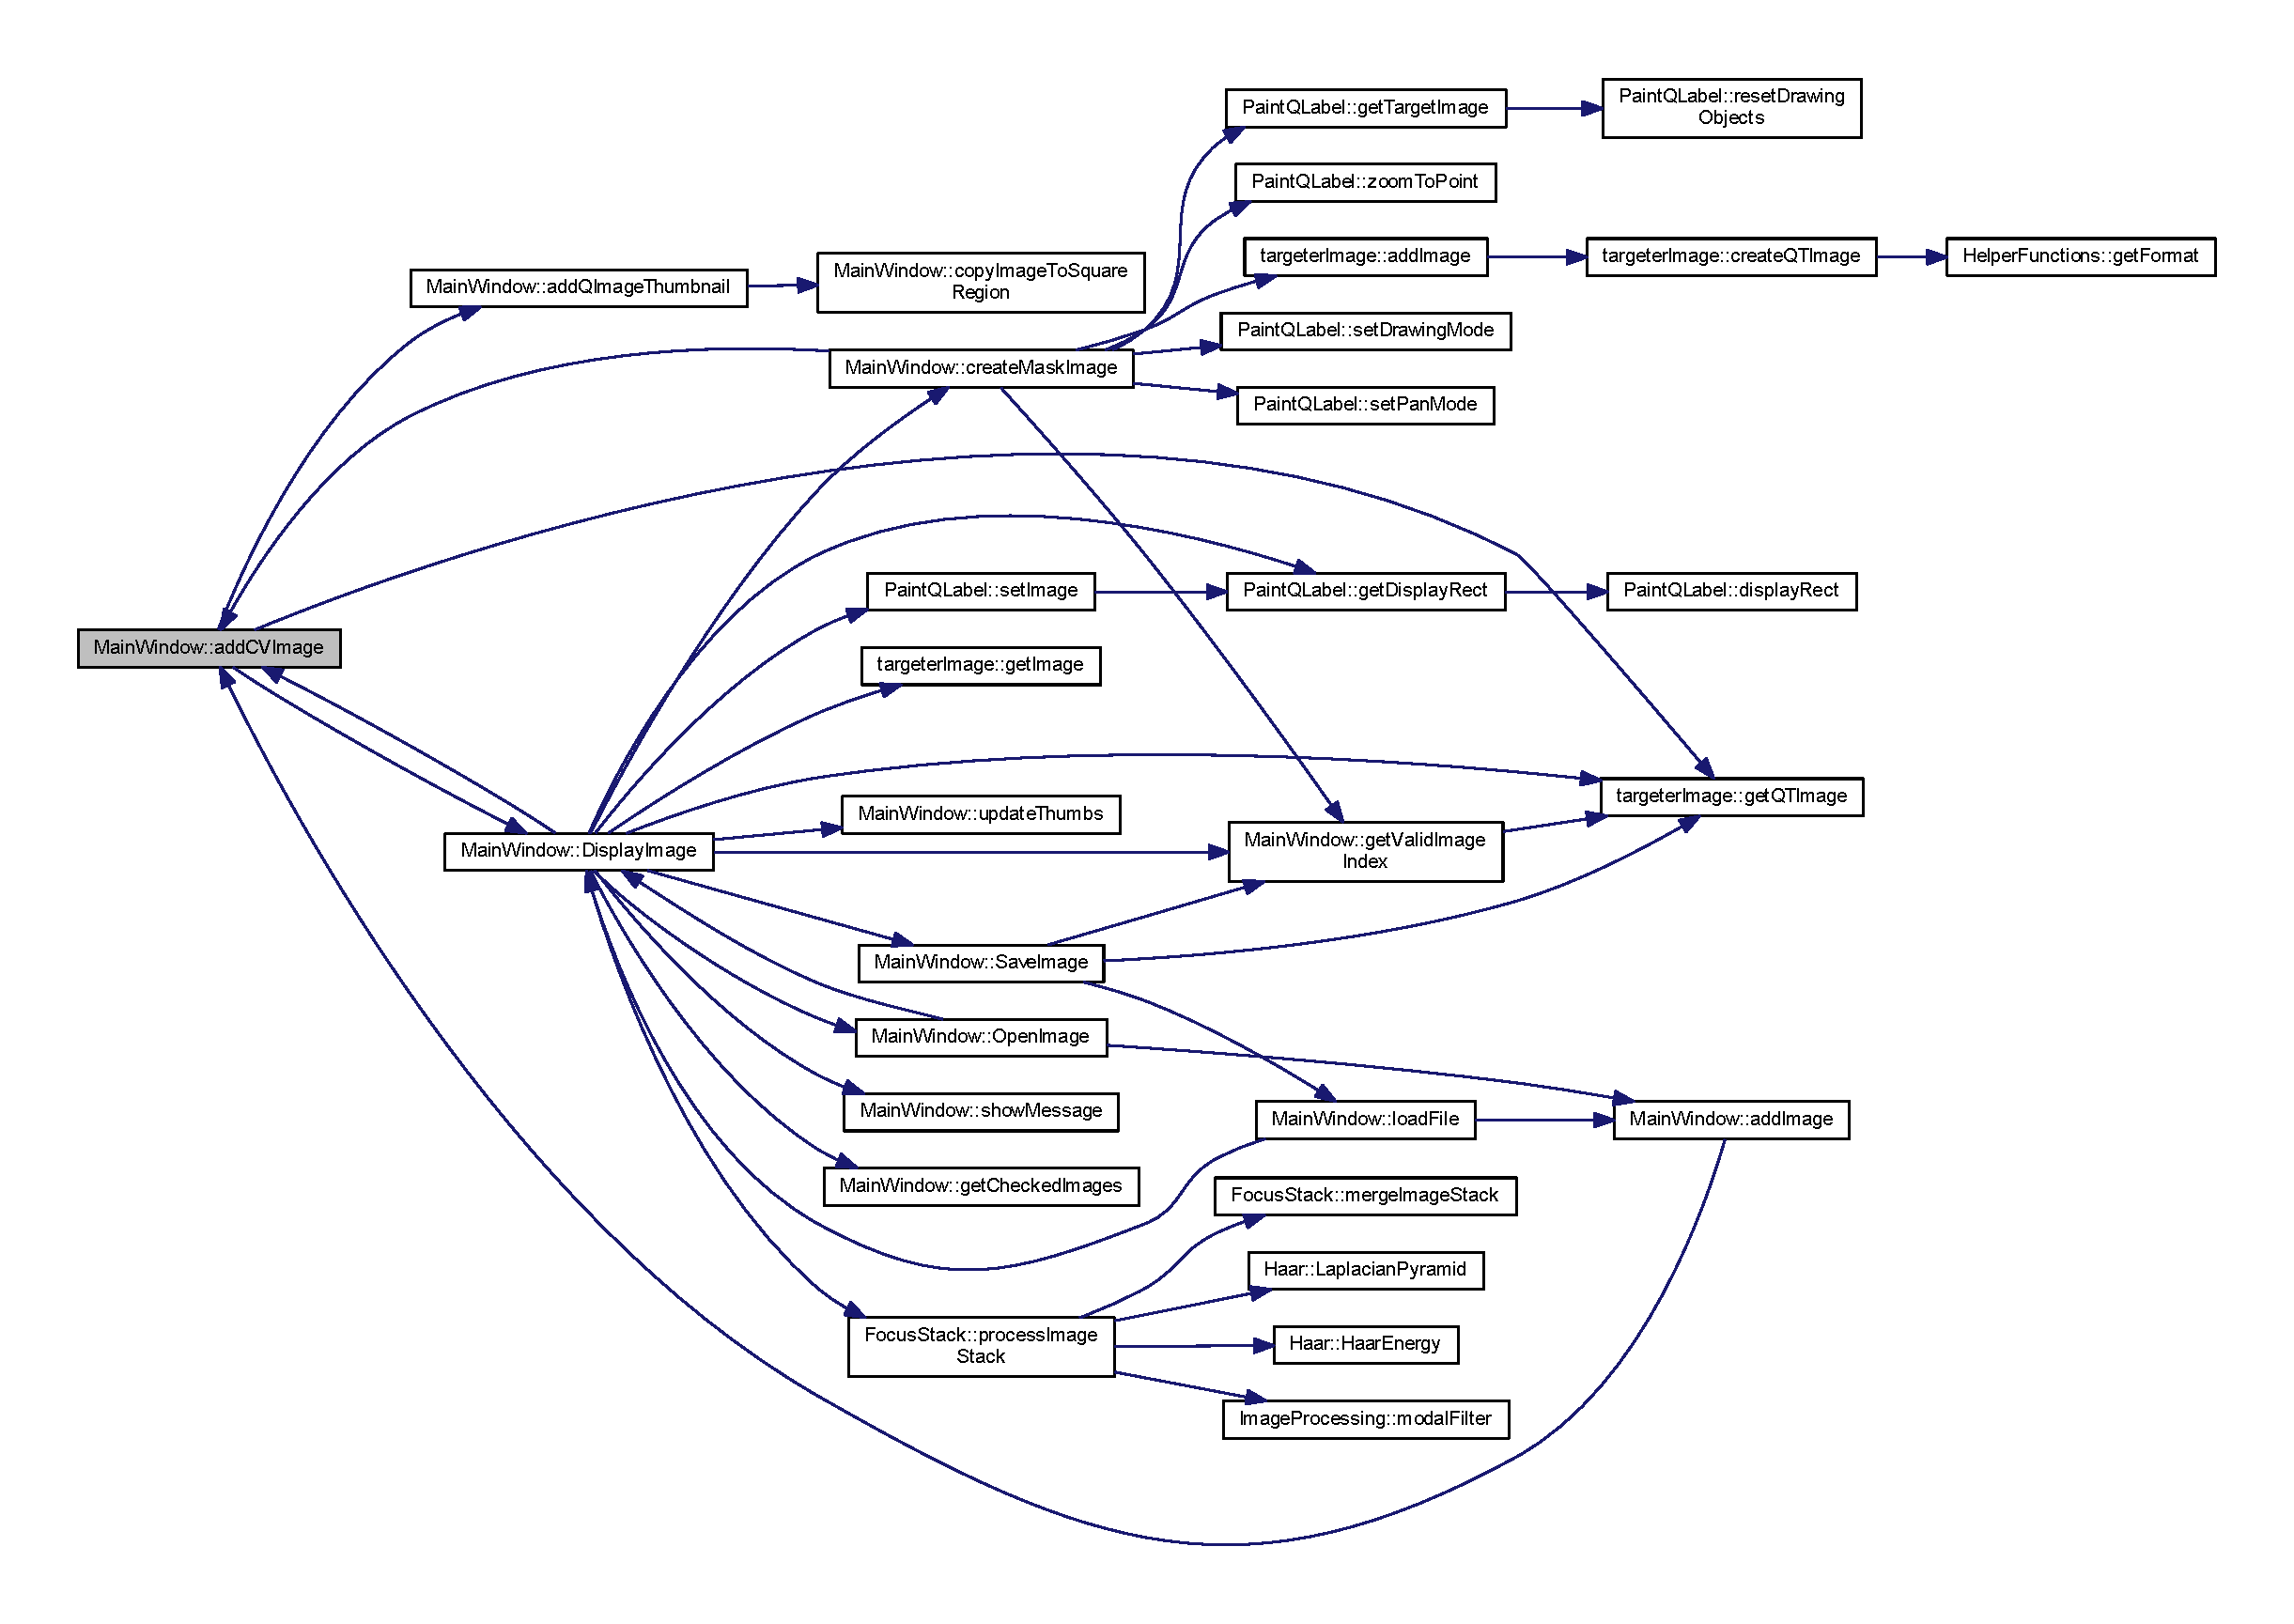
\includegraphics[width=350pt]{class_main_window_a0c29749703b7fc8a64a17d123816bfac_cgraph}
\end{center}
\end{figure}
Here is the caller graph for this function\+:
\nopagebreak
\begin{figure}[H]
\begin{center}
\leavevmode
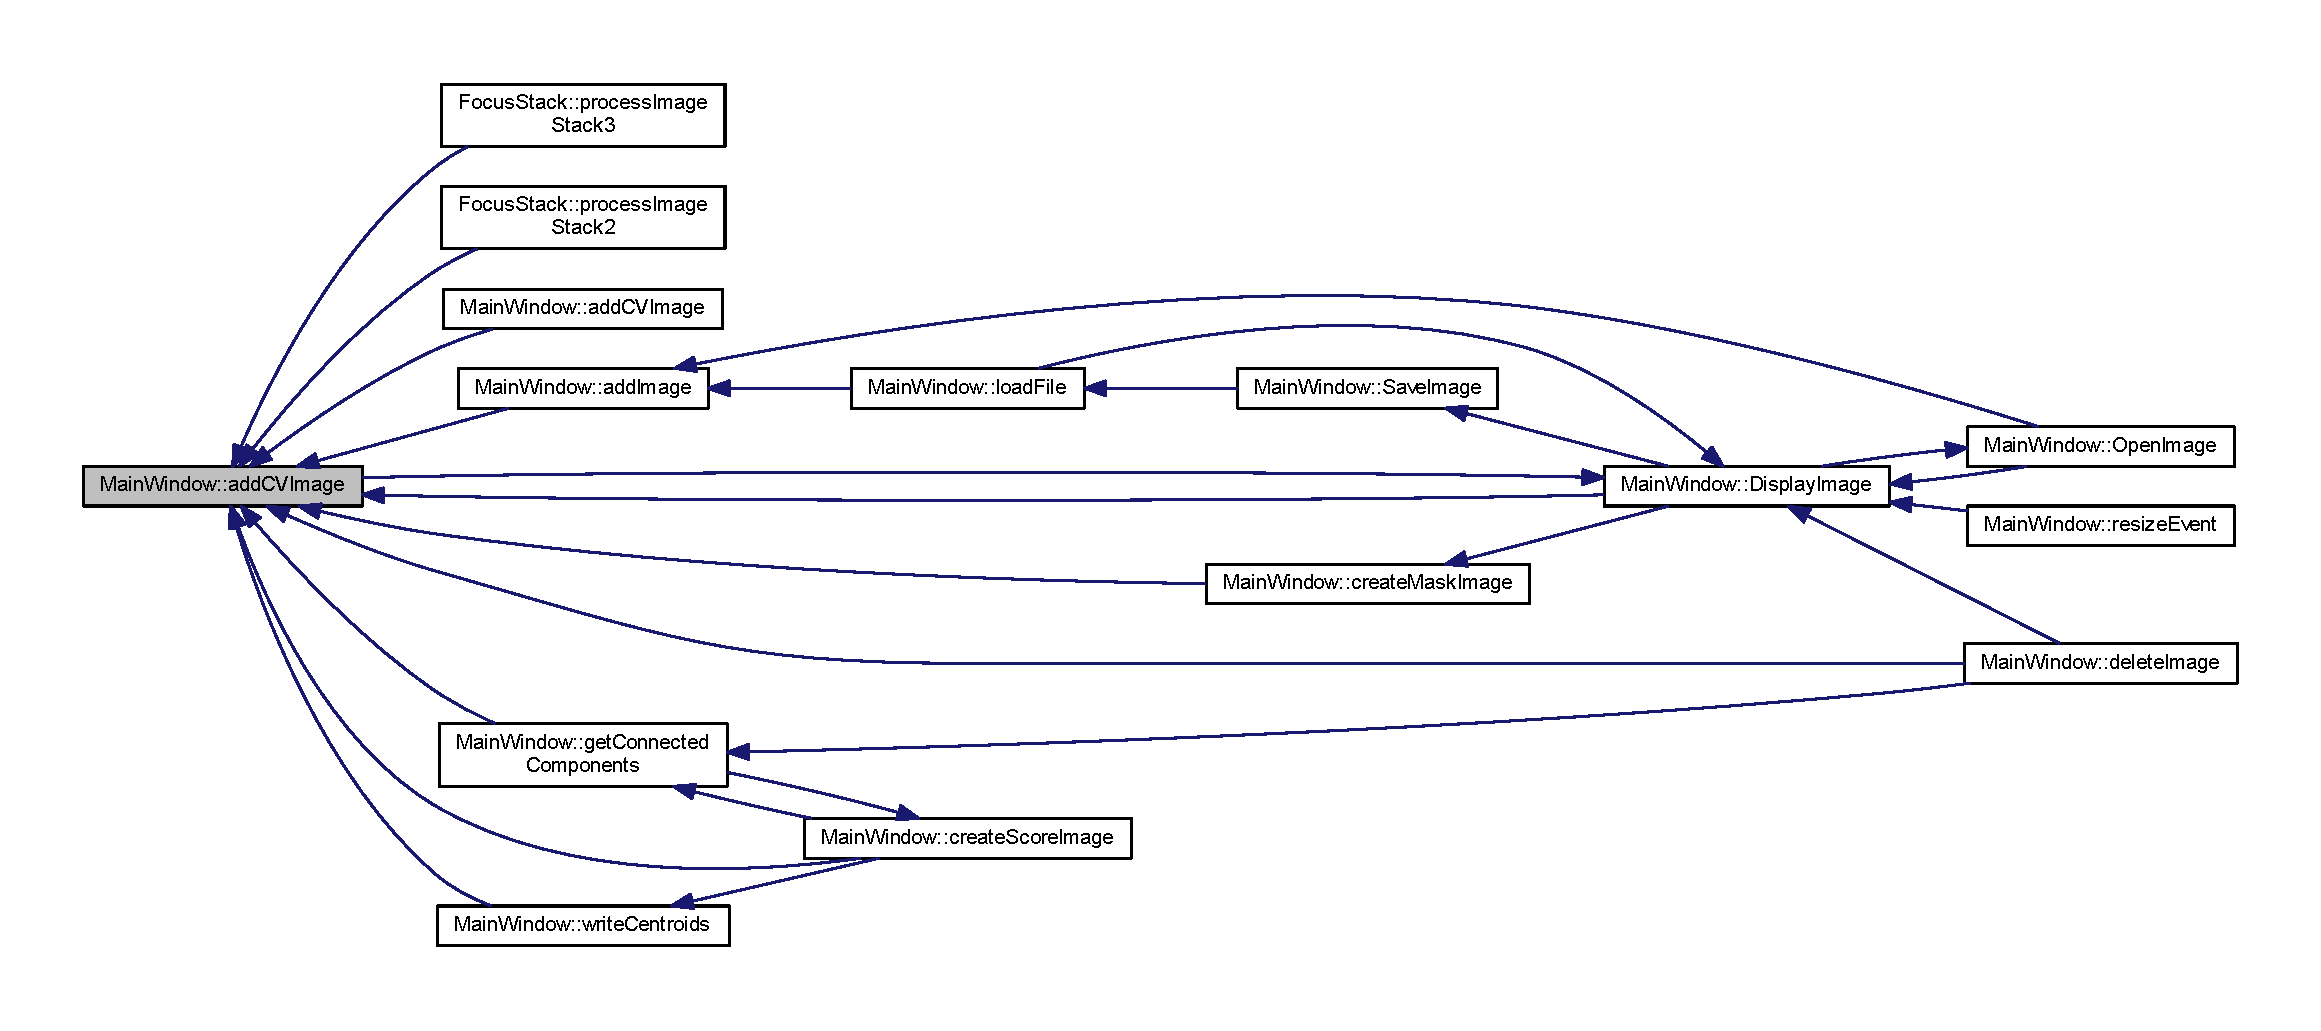
\includegraphics[width=350pt]{class_main_window_a0c29749703b7fc8a64a17d123816bfac_icgraph}
\end{center}
\end{figure}
\mbox{\Hypertarget{class_main_window_ab87edc0e4b2fb3e4fb4df14a8872cbb4}\label{class_main_window_ab87edc0e4b2fb3e4fb4df14a8872cbb4}} 
\index{Main\+Window@{Main\+Window}!add\+C\+V\+Image@{add\+C\+V\+Image}}
\index{add\+C\+V\+Image@{add\+C\+V\+Image}!Main\+Window@{Main\+Window}}
\subsubsection{\texorpdfstring{add\+C\+V\+Image()}{addCVImage()}\hspace{0.1cm}{\footnotesize\ttfamily [2/2]}}
{\footnotesize\ttfamily void Main\+Window\+::add\+C\+V\+Image (\begin{DoxyParamCaption}\item[{cv\+::\+Mat}]{im,  }\item[{Q\+String}]{image\+Name = {\ttfamily \char`\"{}\char`\"{}},  }\item[{bool}]{b\+R\+G\+B\+Swap = {\ttfamily true},  }\item[{image\+Type\+::image\+Type}]{type = {\ttfamily imageType\+:\+:display},  }\item[{bool}]{b\+Display = {\ttfamily true} }\end{DoxyParamCaption})}

Creates targeter image and Q\+Image for display from Open\+CV image

\begin{DoxyAuthor}{Author}
David Watts 
\end{DoxyAuthor}
\begin{DoxySince}{Since}
2017/03/07
\end{DoxySince}
Full\+Name \hyperlink{class_main_window_a0c29749703b7fc8a64a17d123816bfac}{Main\+Window\+::add\+C\+V\+Image} Qualifier 
\begin{DoxyParams}{Parameters}
{\em cv\+::\+Mat} & im \\
\hline
{\em Q\+String} & image\+Name \\
\hline
{\em bool} & b\+R\+G\+B\+Swap \\
\hline
{\em \hyperlink{namespaceimage_type}{image\+Type}} & type \\
\hline
\end{DoxyParams}
\begin{DoxyReturn}{Returns}
void Access public 
\end{DoxyReturn}


Definition at line 568 of file mainwindow.\+cpp.

Here is the call graph for this function\+:
\nopagebreak
\begin{figure}[H]
\begin{center}
\leavevmode
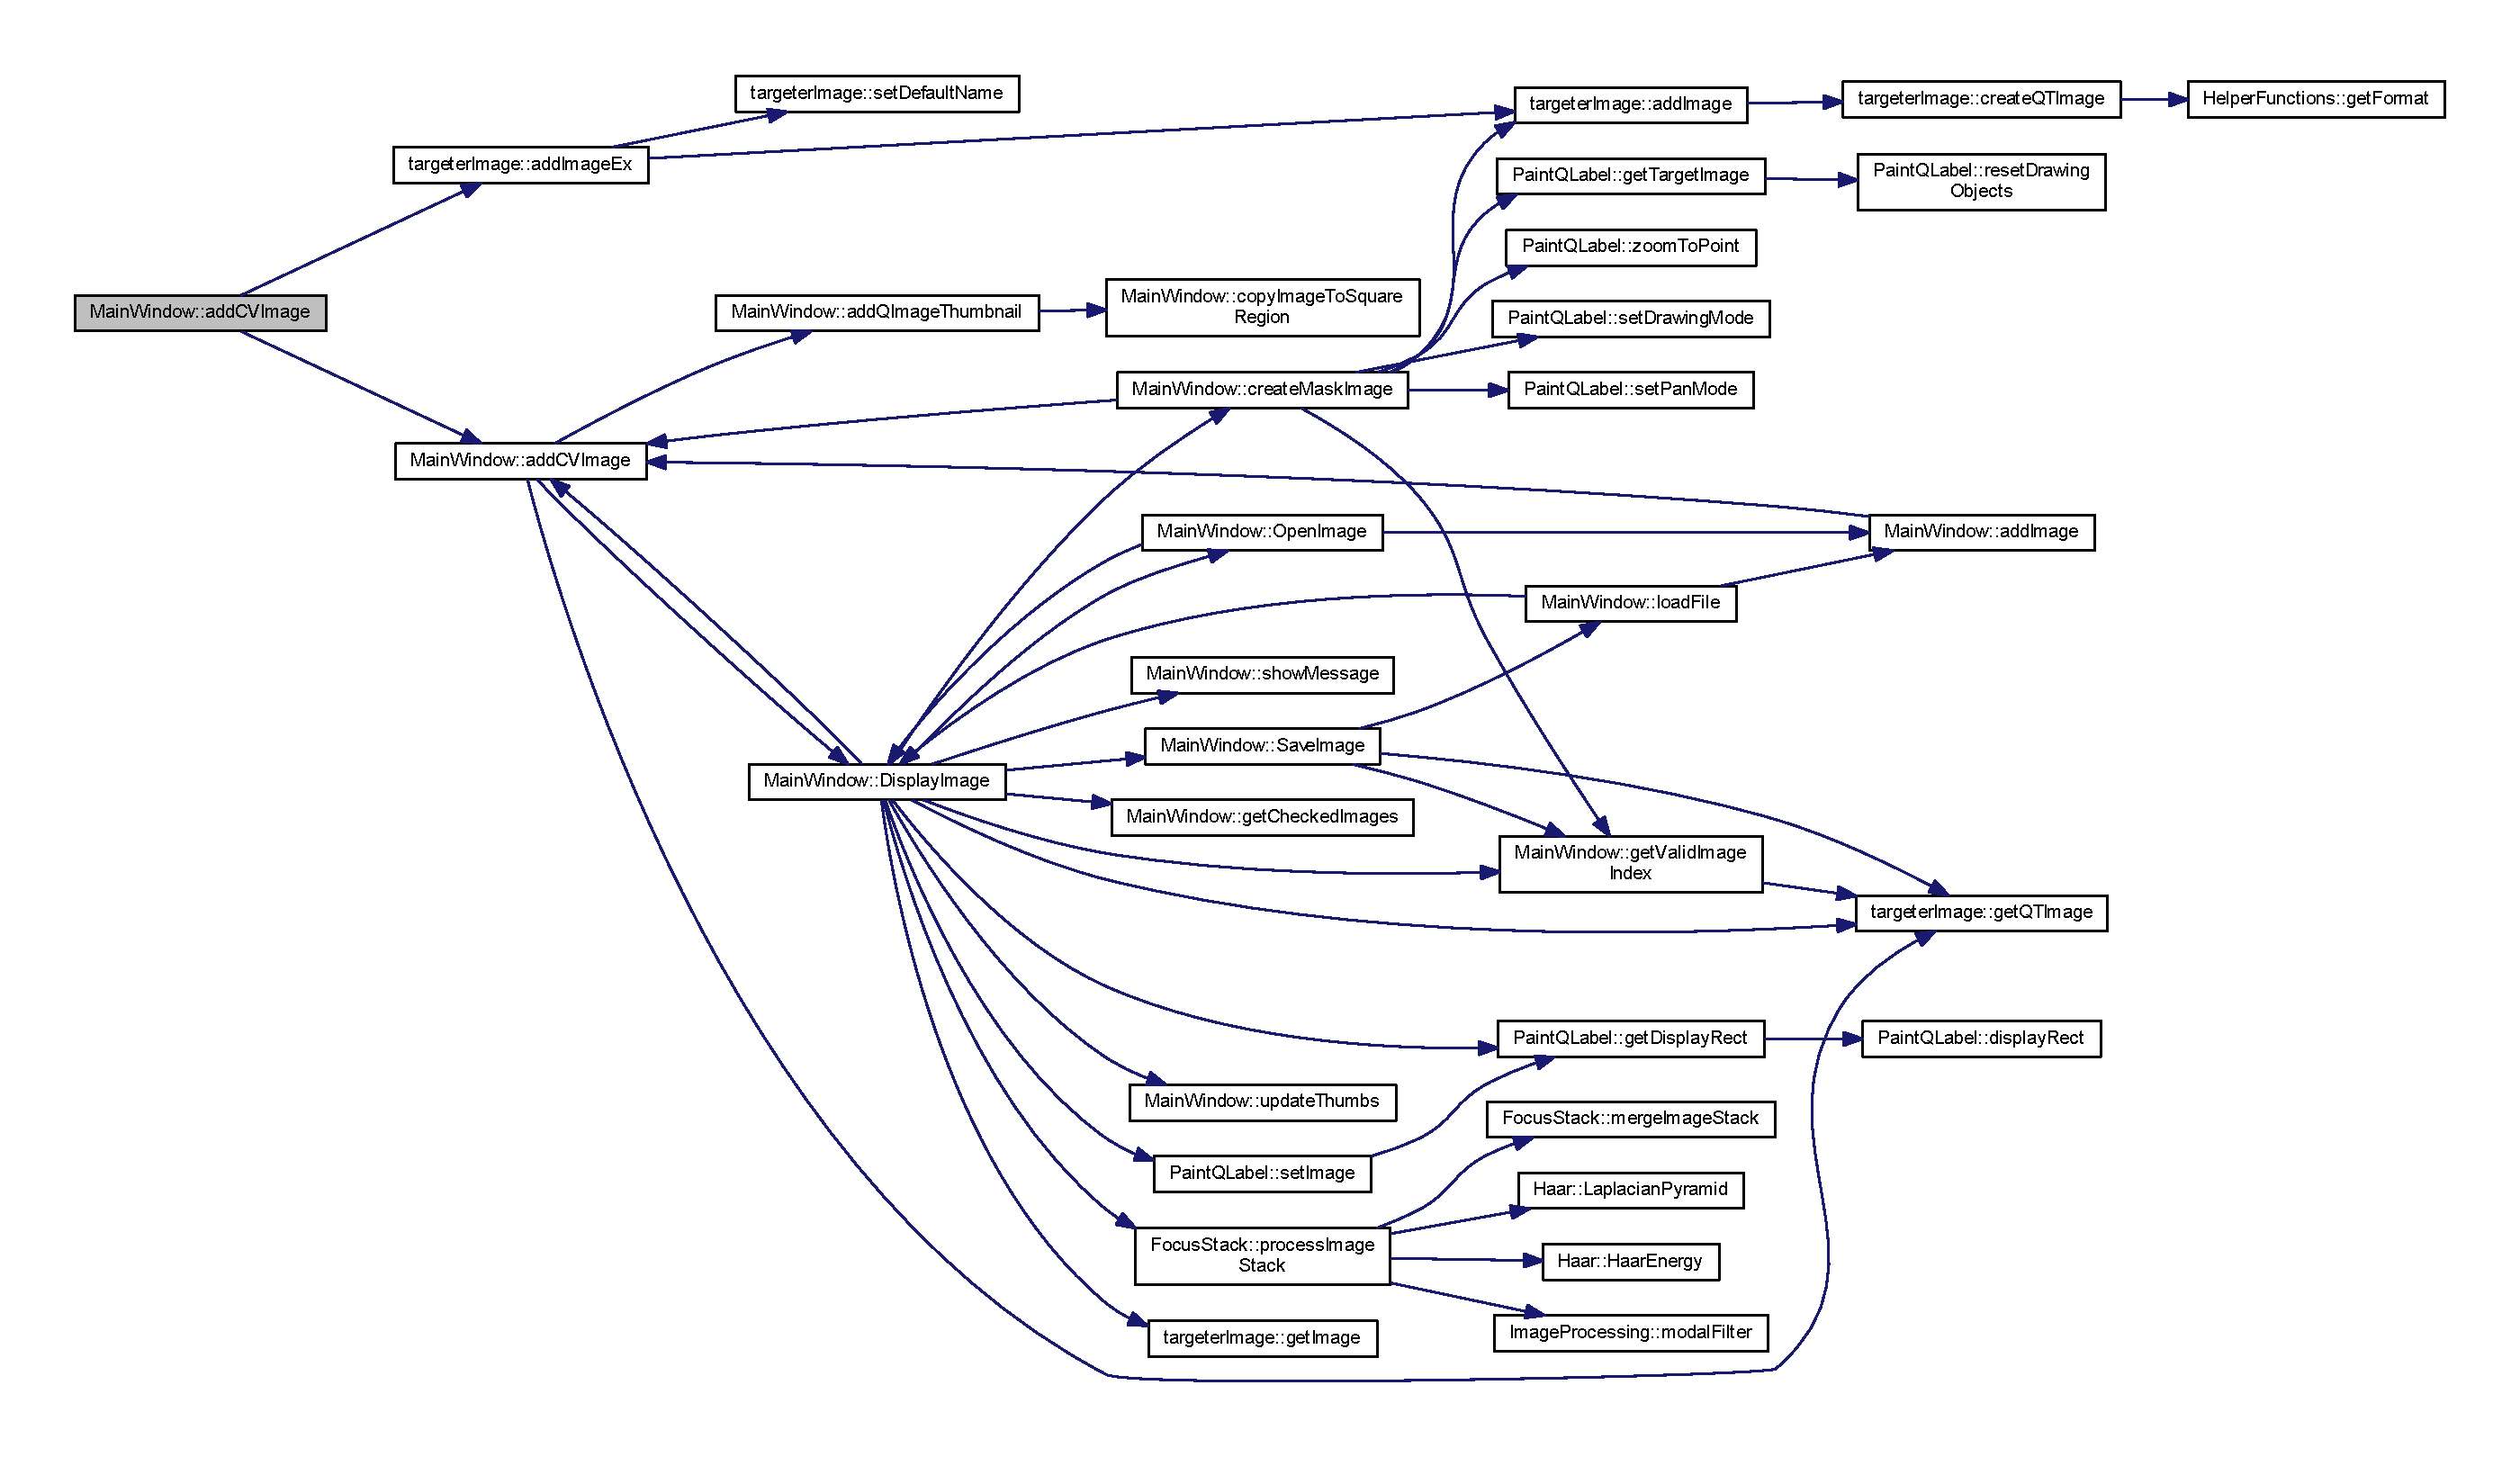
\includegraphics[width=350pt]{class_main_window_ab87edc0e4b2fb3e4fb4df14a8872cbb4_cgraph}
\end{center}
\end{figure}
\mbox{\Hypertarget{class_main_window_ab4d1f49d192d3641e0da68b5a69d014a}\label{class_main_window_ab4d1f49d192d3641e0da68b5a69d014a}} 
\index{Main\+Window@{Main\+Window}!add\+Image@{add\+Image}}
\index{add\+Image@{add\+Image}!Main\+Window@{Main\+Window}}
\subsubsection{\texorpdfstring{add\+Image()}{addImage()}}
{\footnotesize\ttfamily void Main\+Window\+::add\+Image (\begin{DoxyParamCaption}\item[{const Q\+String \&}]{file\+Name,  }\item[{image\+Type\+::image\+Type}]{type = {\ttfamily imageType\+:\+:display} }\end{DoxyParamCaption})}

Given a file name loads and reads image

\begin{DoxyAuthor}{Author}
David Watts 
\end{DoxyAuthor}
\begin{DoxySince}{Since}
2017/03/07
\end{DoxySince}
Full\+Name \hyperlink{class_main_window_ab4d1f49d192d3641e0da68b5a69d014a}{Main\+Window\+::add\+Image} Qualifier 
\begin{DoxyParams}{Parameters}
{\em const} & Q\+String \& file\+Name \\
\hline
{\em \hyperlink{namespaceimage_type}{image\+Type}} & type \\
\hline
\end{DoxyParams}
\begin{DoxyReturn}{Returns}
void Access public 
\end{DoxyReturn}


Definition at line 625 of file mainwindow.\+cpp.

Here is the call graph for this function\+:
\nopagebreak
\begin{figure}[H]
\begin{center}
\leavevmode
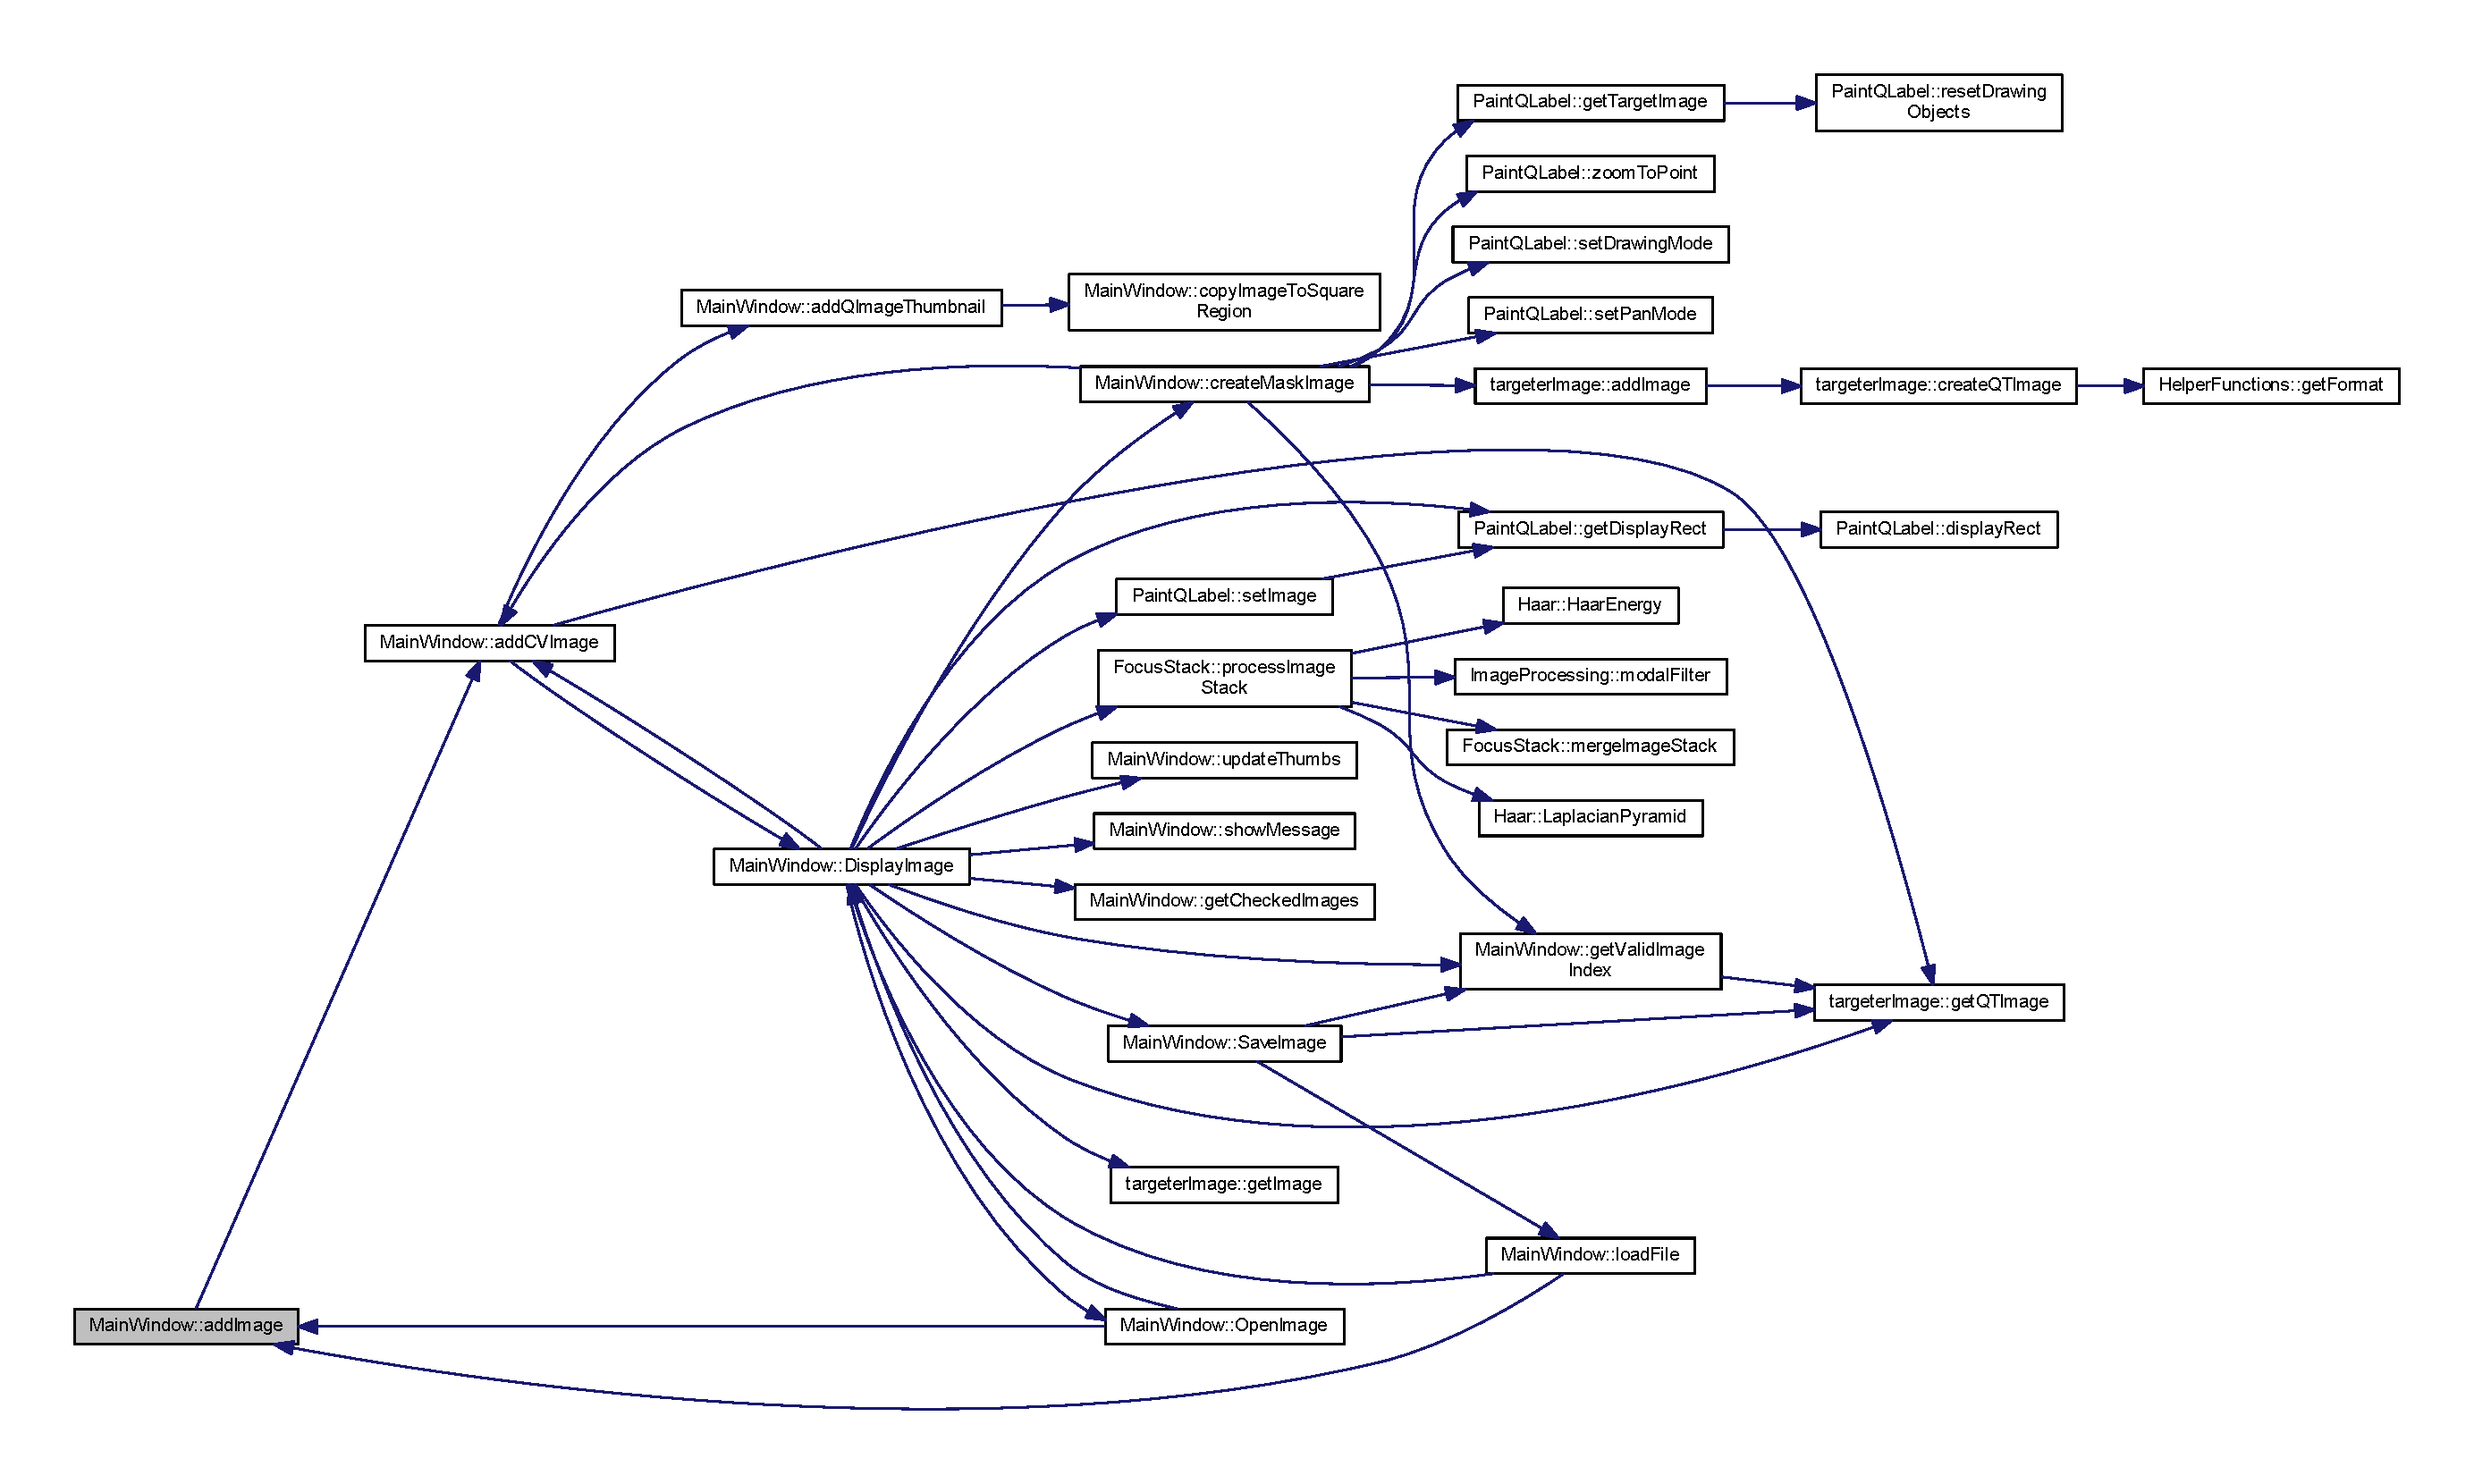
\includegraphics[width=350pt]{class_main_window_ab4d1f49d192d3641e0da68b5a69d014a_cgraph}
\end{center}
\end{figure}
Here is the caller graph for this function\+:
\nopagebreak
\begin{figure}[H]
\begin{center}
\leavevmode
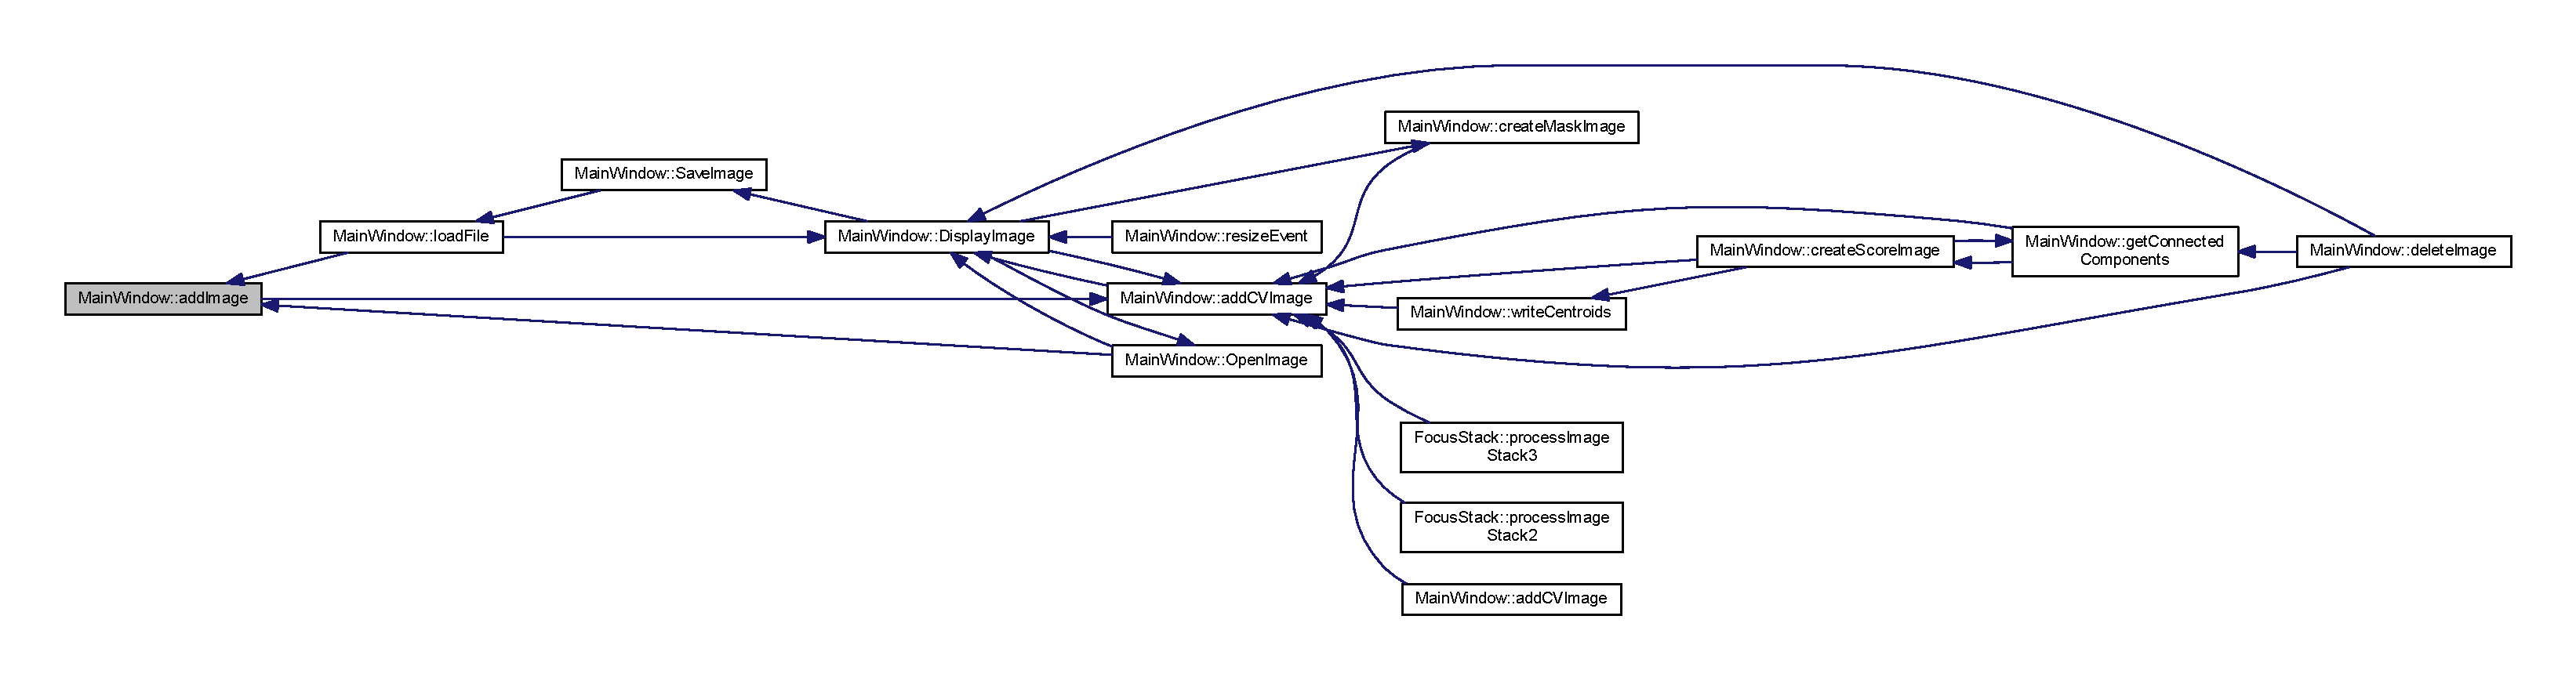
\includegraphics[width=350pt]{class_main_window_ab4d1f49d192d3641e0da68b5a69d014a_icgraph}
\end{center}
\end{figure}
\mbox{\Hypertarget{class_main_window_a8b60c57f82b0ac86df7c64692294a35e}\label{class_main_window_a8b60c57f82b0ac86df7c64692294a35e}} 
\index{Main\+Window@{Main\+Window}!add\+Q\+Image\+Thumbnail@{add\+Q\+Image\+Thumbnail}}
\index{add\+Q\+Image\+Thumbnail@{add\+Q\+Image\+Thumbnail}!Main\+Window@{Main\+Window}}
\subsubsection{\texorpdfstring{add\+Q\+Image\+Thumbnail()}{addQImageThumbnail()}}
{\footnotesize\ttfamily void Main\+Window\+::add\+Q\+Image\+Thumbnail (\begin{DoxyParamCaption}\item[{Q\+Image \&}]{qim,  }\item[{Q\+String}]{image\+Name = {\ttfamily \char`\"{}\char`\"{}},  }\item[{image\+Type\+::image\+Type}]{type = {\ttfamily imageType\+:\+:display} }\end{DoxyParamCaption})}

adds Q\+Image to thumbnail list

\begin{DoxyAuthor}{Author}
David Watts 
\end{DoxyAuthor}
\begin{DoxySince}{Since}
2017/03/07
\end{DoxySince}
Full\+Name Main\+Window\+::add\+Q\+Image Qualifier 
\begin{DoxyParams}{Parameters}
{\em Q\+Image} & \& qim \\
\hline
{\em Q\+String} & image\+Name \\
\hline
{\em \hyperlink{namespaceimage_type}{image\+Type}} & type \\
\hline
\end{DoxyParams}
\begin{DoxyReturn}{Returns}
void Access public 
\end{DoxyReturn}


Definition at line 739 of file mainwindow.\+cpp.

Here is the call graph for this function\+:
\nopagebreak
\begin{figure}[H]
\begin{center}
\leavevmode
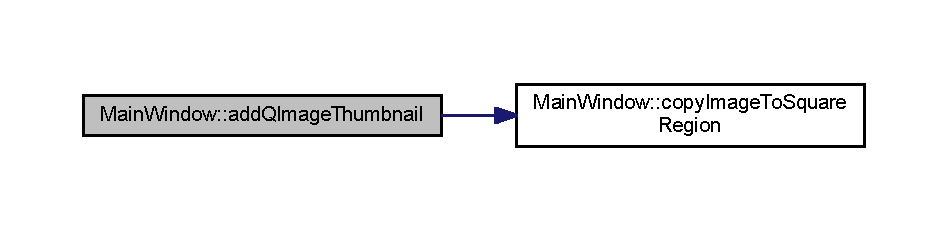
\includegraphics[width=350pt]{class_main_window_a8b60c57f82b0ac86df7c64692294a35e_cgraph}
\end{center}
\end{figure}
Here is the caller graph for this function\+:
\nopagebreak
\begin{figure}[H]
\begin{center}
\leavevmode
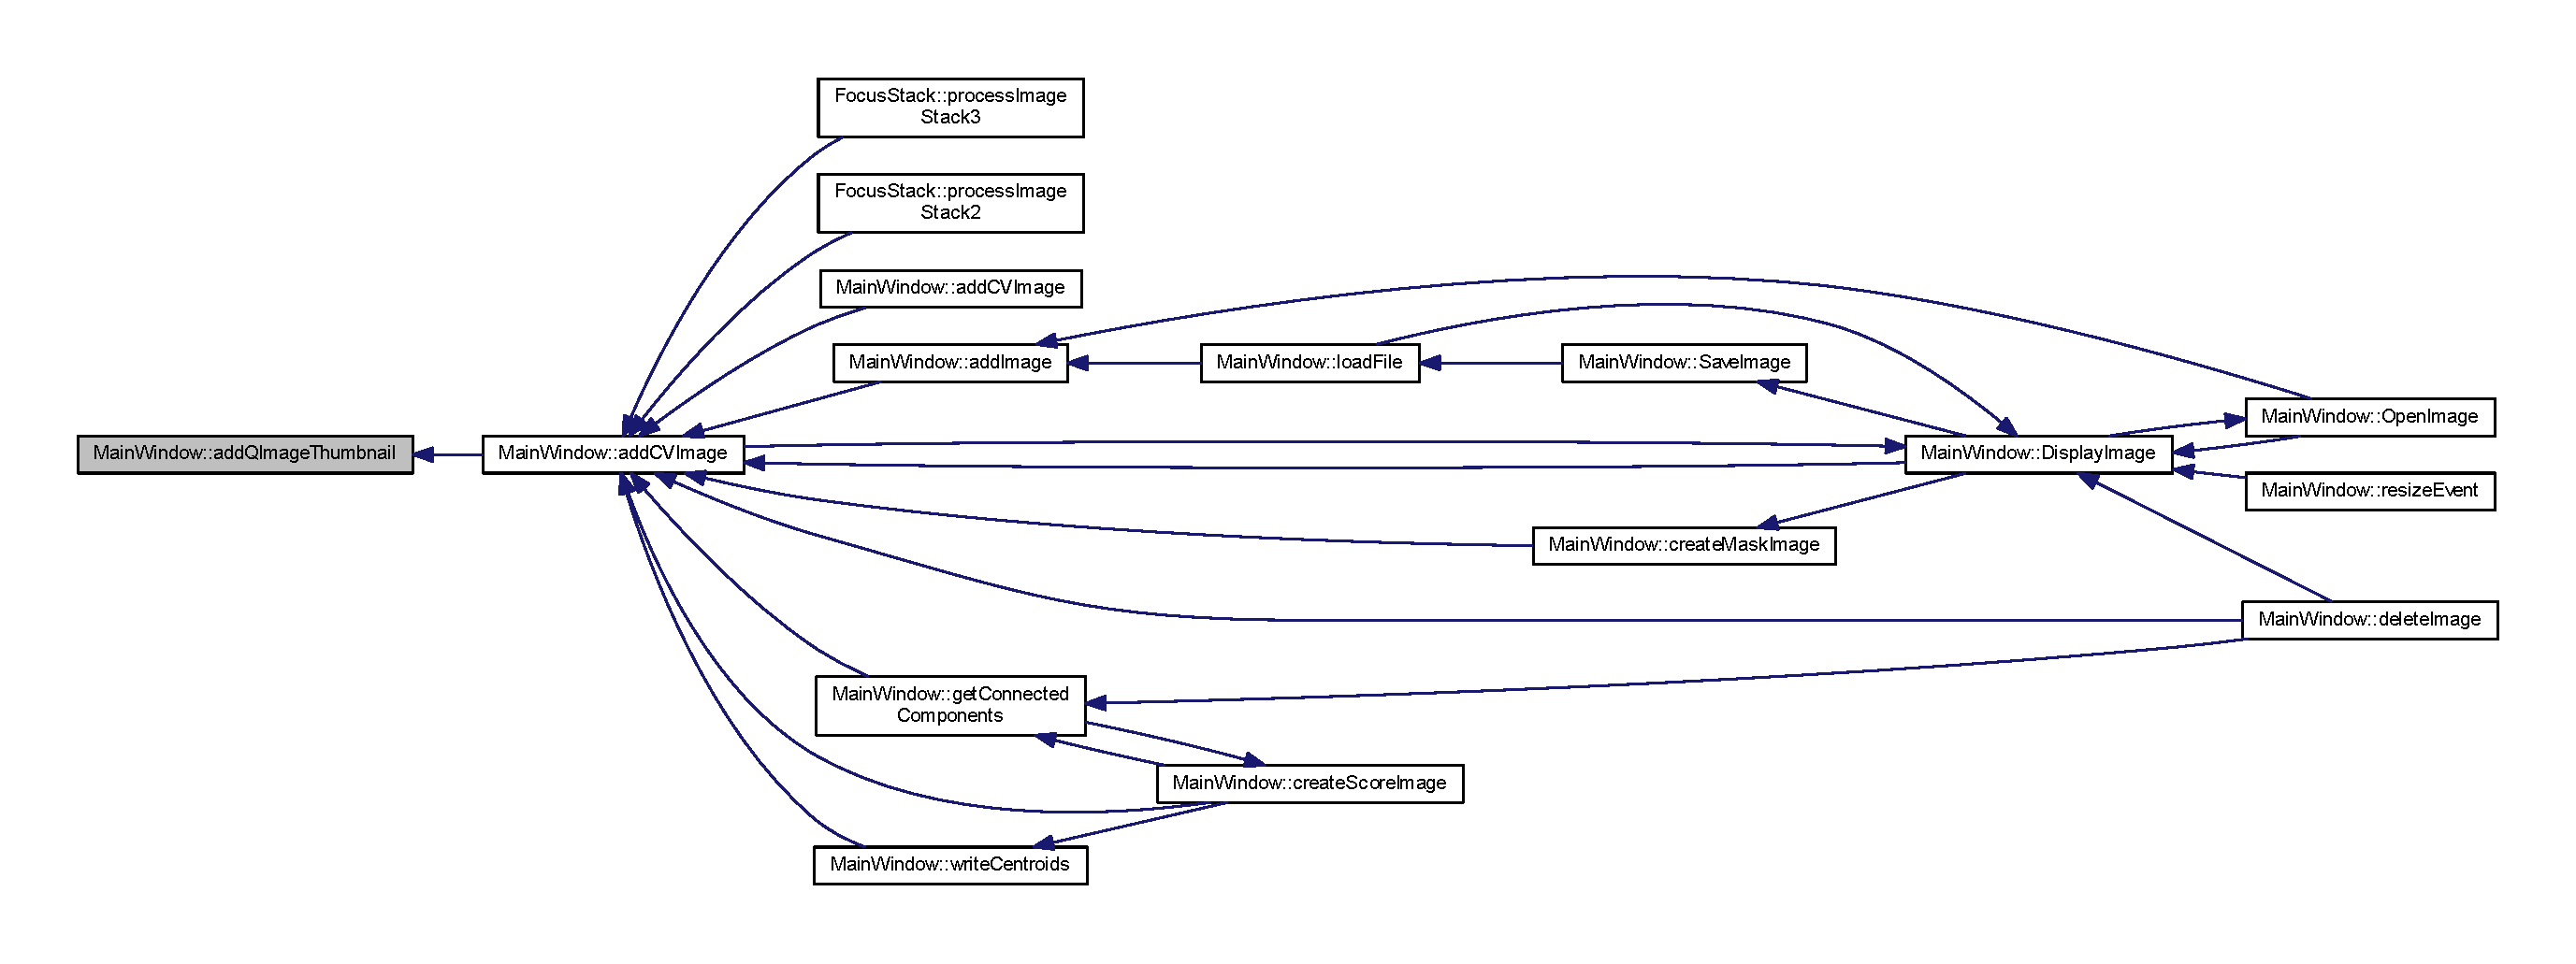
\includegraphics[width=350pt]{class_main_window_a8b60c57f82b0ac86df7c64692294a35e_icgraph}
\end{center}
\end{figure}
\mbox{\Hypertarget{class_main_window_a5e034c81127e2a14248eb81414e1e96e}\label{class_main_window_a5e034c81127e2a14248eb81414e1e96e}} 
\index{Main\+Window@{Main\+Window}!copy\+Image\+To\+Square\+Region@{copy\+Image\+To\+Square\+Region}}
\index{copy\+Image\+To\+Square\+Region@{copy\+Image\+To\+Square\+Region}!Main\+Window@{Main\+Window}}
\subsubsection{\texorpdfstring{copy\+Image\+To\+Square\+Region()}{copyImageToSquareRegion()}}
{\footnotesize\ttfamily Q\+Image Main\+Window\+::copy\+Image\+To\+Square\+Region (\begin{DoxyParamCaption}\item[{Q\+Image}]{qim,  }\item[{Q\+Color}]{col }\end{DoxyParamCaption})}

Makes sub image from rectangular region of image

\begin{DoxyAuthor}{Author}
David Watts 
\end{DoxyAuthor}
\begin{DoxySince}{Since}
2017/03/07
\end{DoxySince}
Full\+Name \hyperlink{class_main_window_a5e034c81127e2a14248eb81414e1e96e}{Main\+Window\+::copy\+Image\+To\+Square\+Region} Qualifier 
\begin{DoxyParams}{Parameters}
{\em Q\+Image} & qim \\
\hline
{\em Q\+Color} & col \\
\hline
\end{DoxyParams}
\begin{DoxyReturn}{Returns}
Q\+T\+\_\+\+N\+A\+M\+E\+S\+P\+A\+C\+E\+::\+Q\+Image Access public 
\end{DoxyReturn}


Definition at line 656 of file mainwindow.\+cpp.

Here is the caller graph for this function\+:
\nopagebreak
\begin{figure}[H]
\begin{center}
\leavevmode
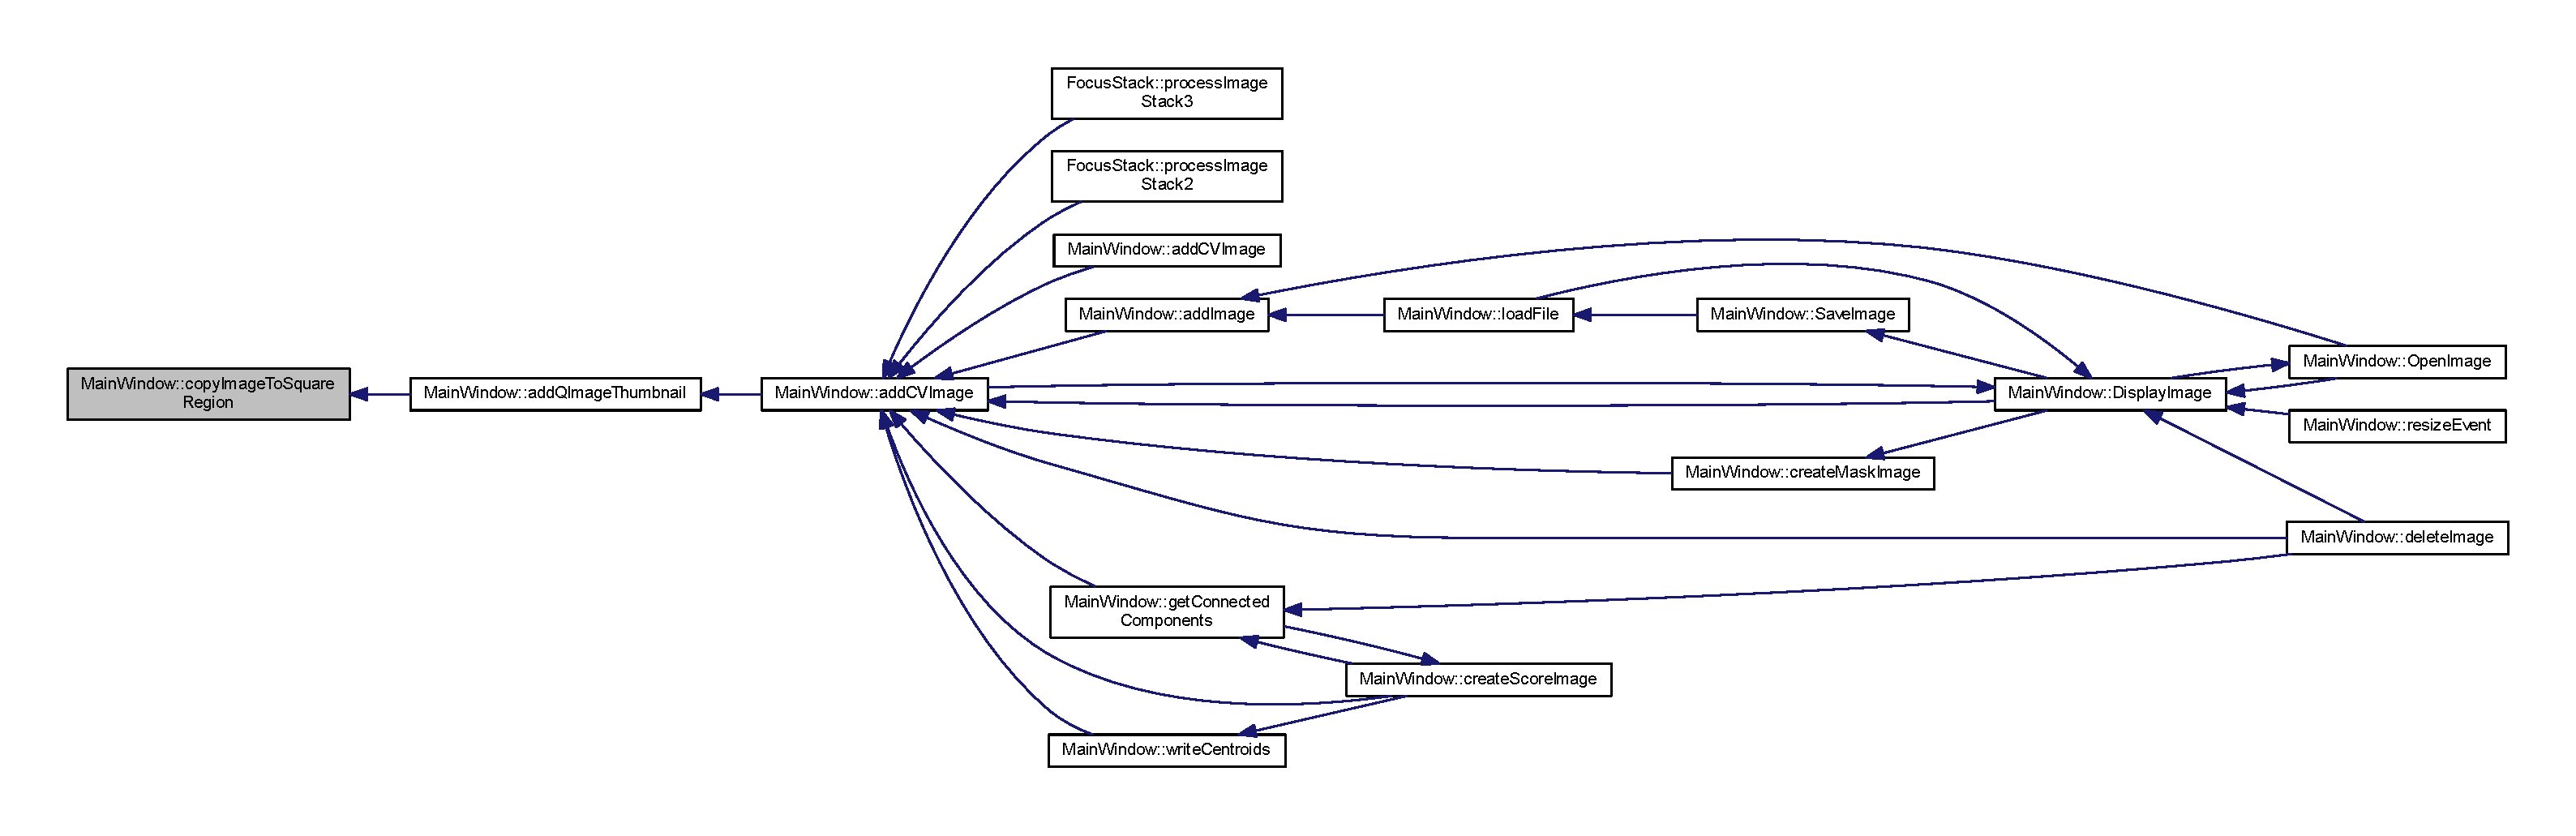
\includegraphics[width=350pt]{class_main_window_a5e034c81127e2a14248eb81414e1e96e_icgraph}
\end{center}
\end{figure}
\mbox{\Hypertarget{class_main_window_a92a40847027eaf2cf258c3a9f8da4c48}\label{class_main_window_a92a40847027eaf2cf258c3a9f8da4c48}} 
\index{Main\+Window@{Main\+Window}!create\+Mask\+Image@{create\+Mask\+Image}}
\index{create\+Mask\+Image@{create\+Mask\+Image}!Main\+Window@{Main\+Window}}
\subsubsection{\texorpdfstring{create\+Mask\+Image()}{createMaskImage()}}
{\footnotesize\ttfamily void Main\+Window\+::create\+Mask\+Image (\begin{DoxyParamCaption}\item[{cv\+::\+Mat}]{im,  }\item[{\hyperlink{structdrawing_shape}{drawing\+Shape}}]{shape }\end{DoxyParamCaption})}

Gets binary mask image and sub image from region from drawing object shape

\begin{DoxyAuthor}{Author}
David Watts 
\end{DoxyAuthor}
\begin{DoxySince}{Since}
2017/03/07
\end{DoxySince}
Full\+Name Main\+Window\+::mask\+Image Qualifier 
\begin{DoxyParams}{Parameters}
{\em Mat} & im \\
\hline
{\em \hyperlink{structdrawing_shape}{drawing\+Shape}} & shape \\
\hline
{\em \hyperlink{classtargeter_image}{targeter\+Image}} & \& tim \\
\hline
\end{DoxyParams}
\begin{DoxyReturn}{Returns}
void Access public 
\end{DoxyReturn}


Definition at line 1253 of file mainwindow.\+cpp.

Here is the call graph for this function\+:
\nopagebreak
\begin{figure}[H]
\begin{center}
\leavevmode
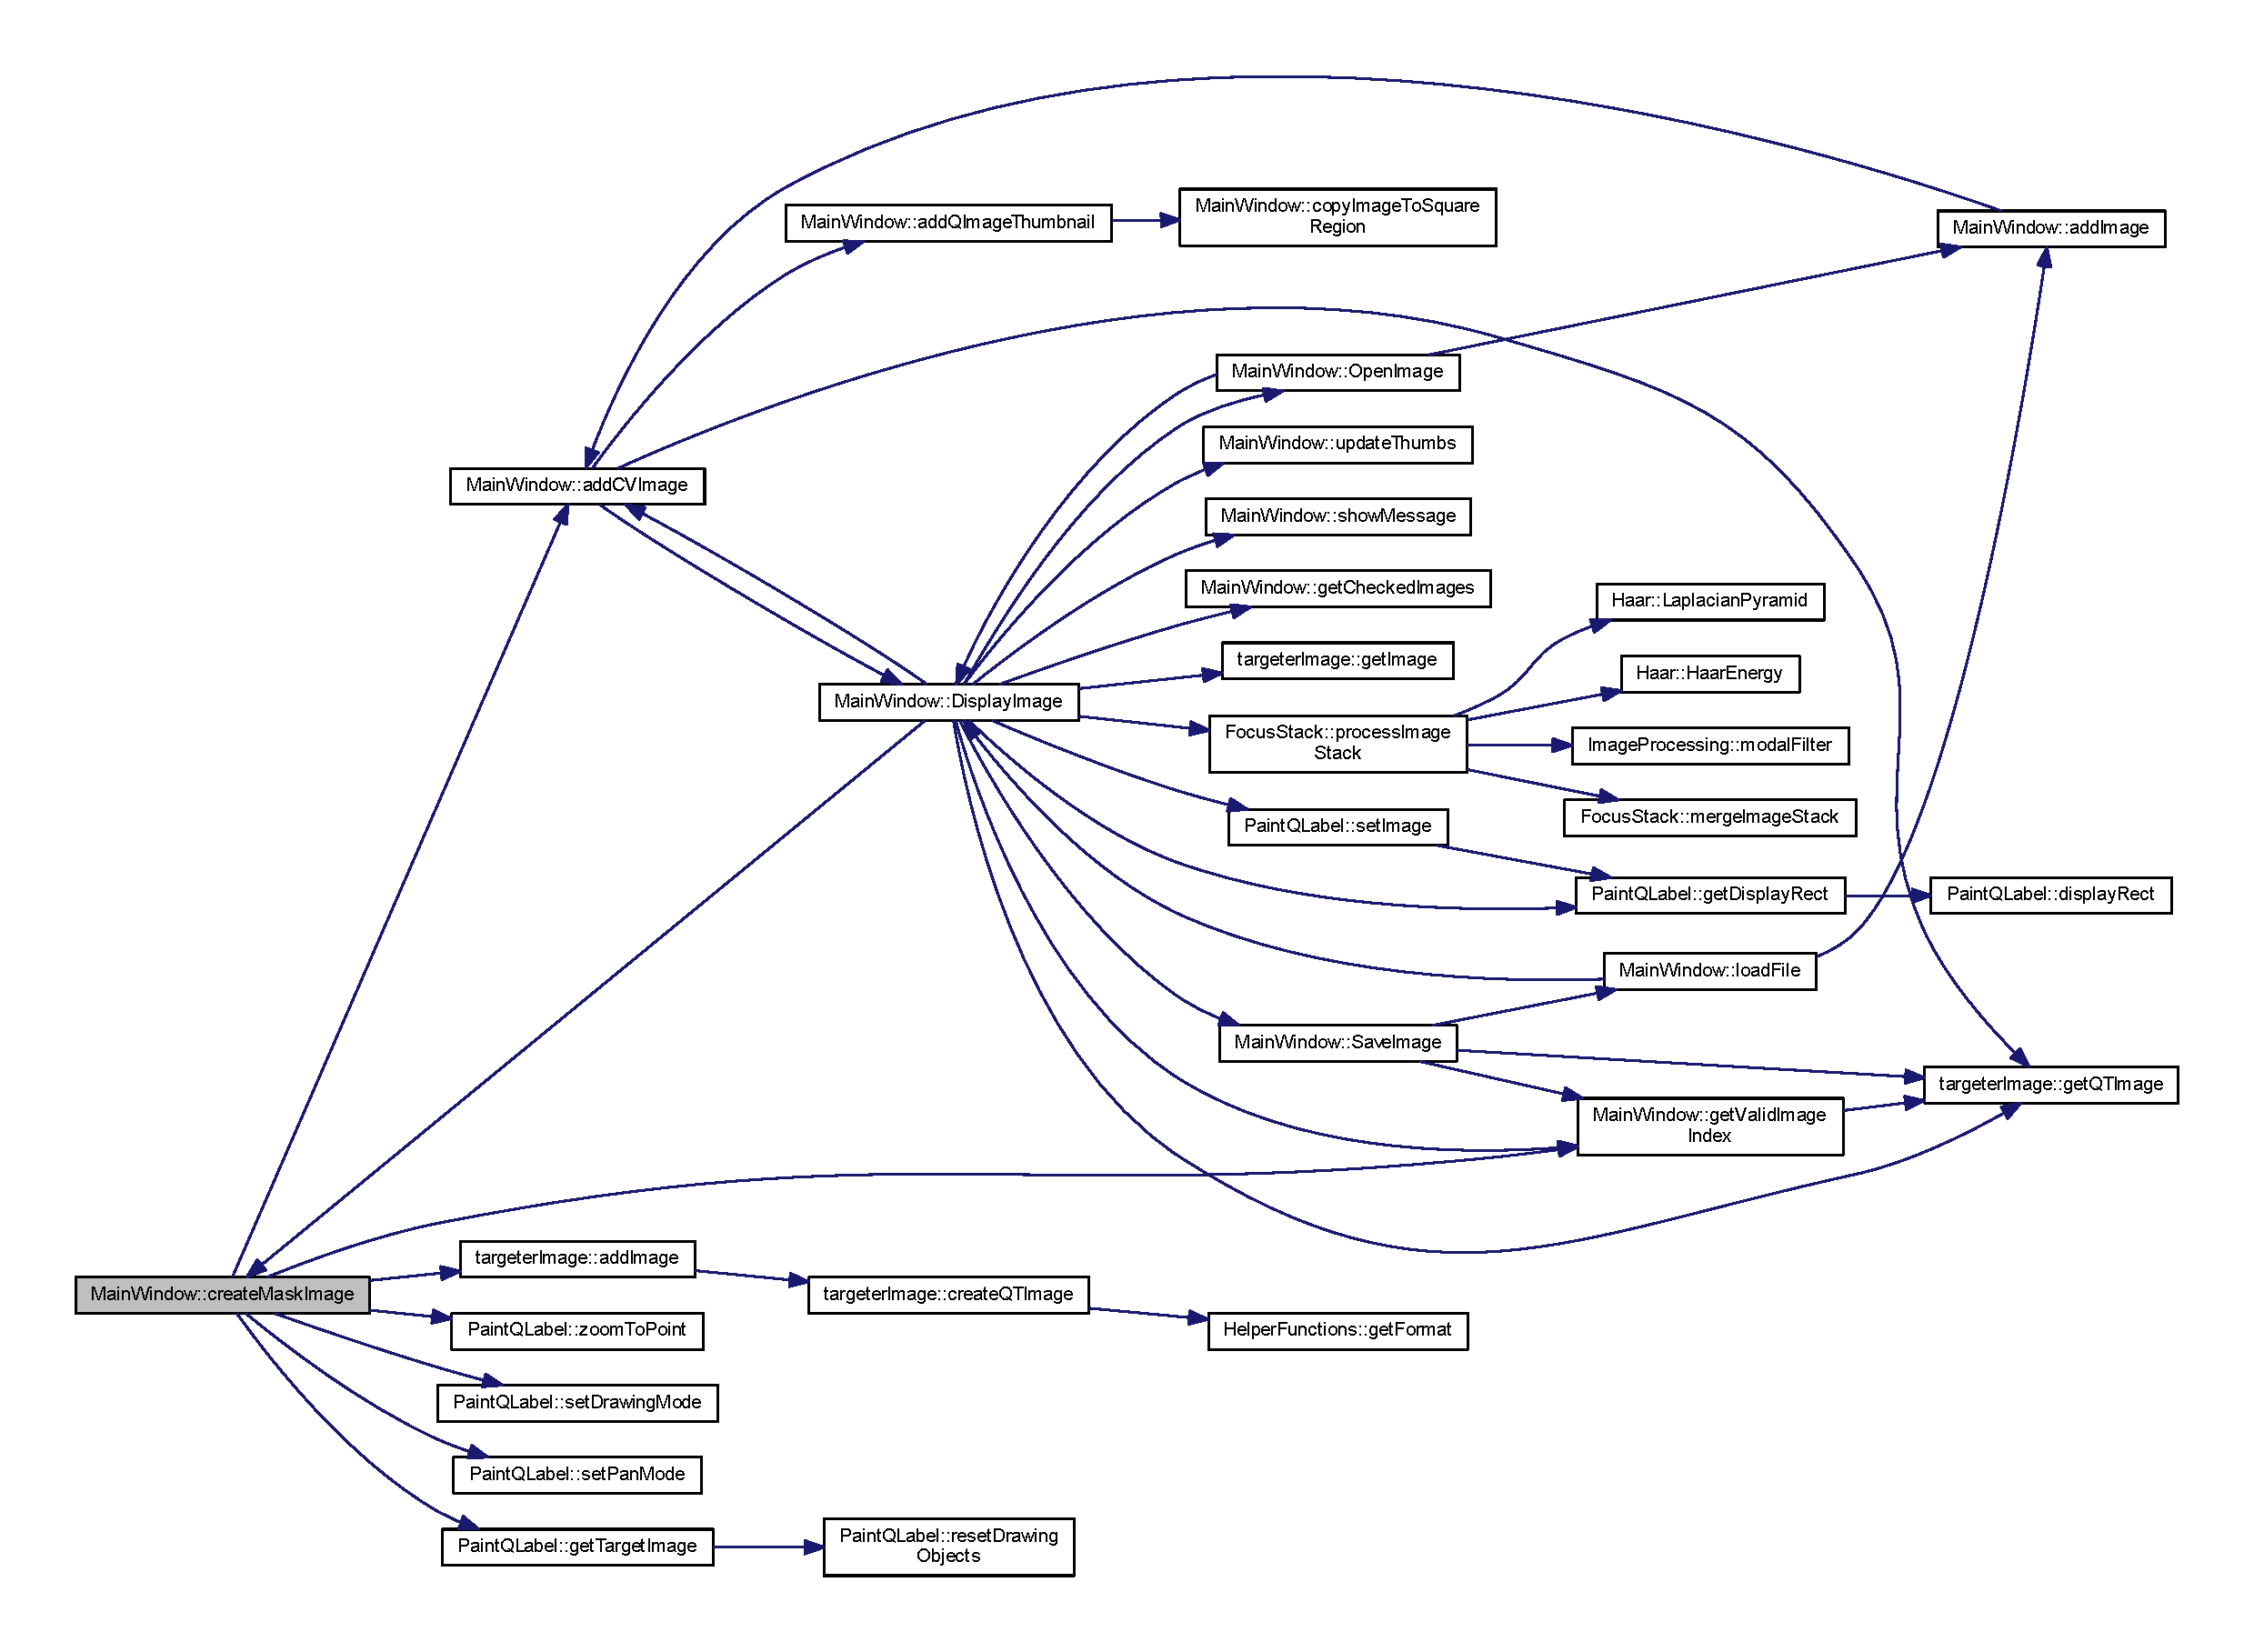
\includegraphics[width=350pt]{class_main_window_a92a40847027eaf2cf258c3a9f8da4c48_cgraph}
\end{center}
\end{figure}
Here is the caller graph for this function\+:
\nopagebreak
\begin{figure}[H]
\begin{center}
\leavevmode
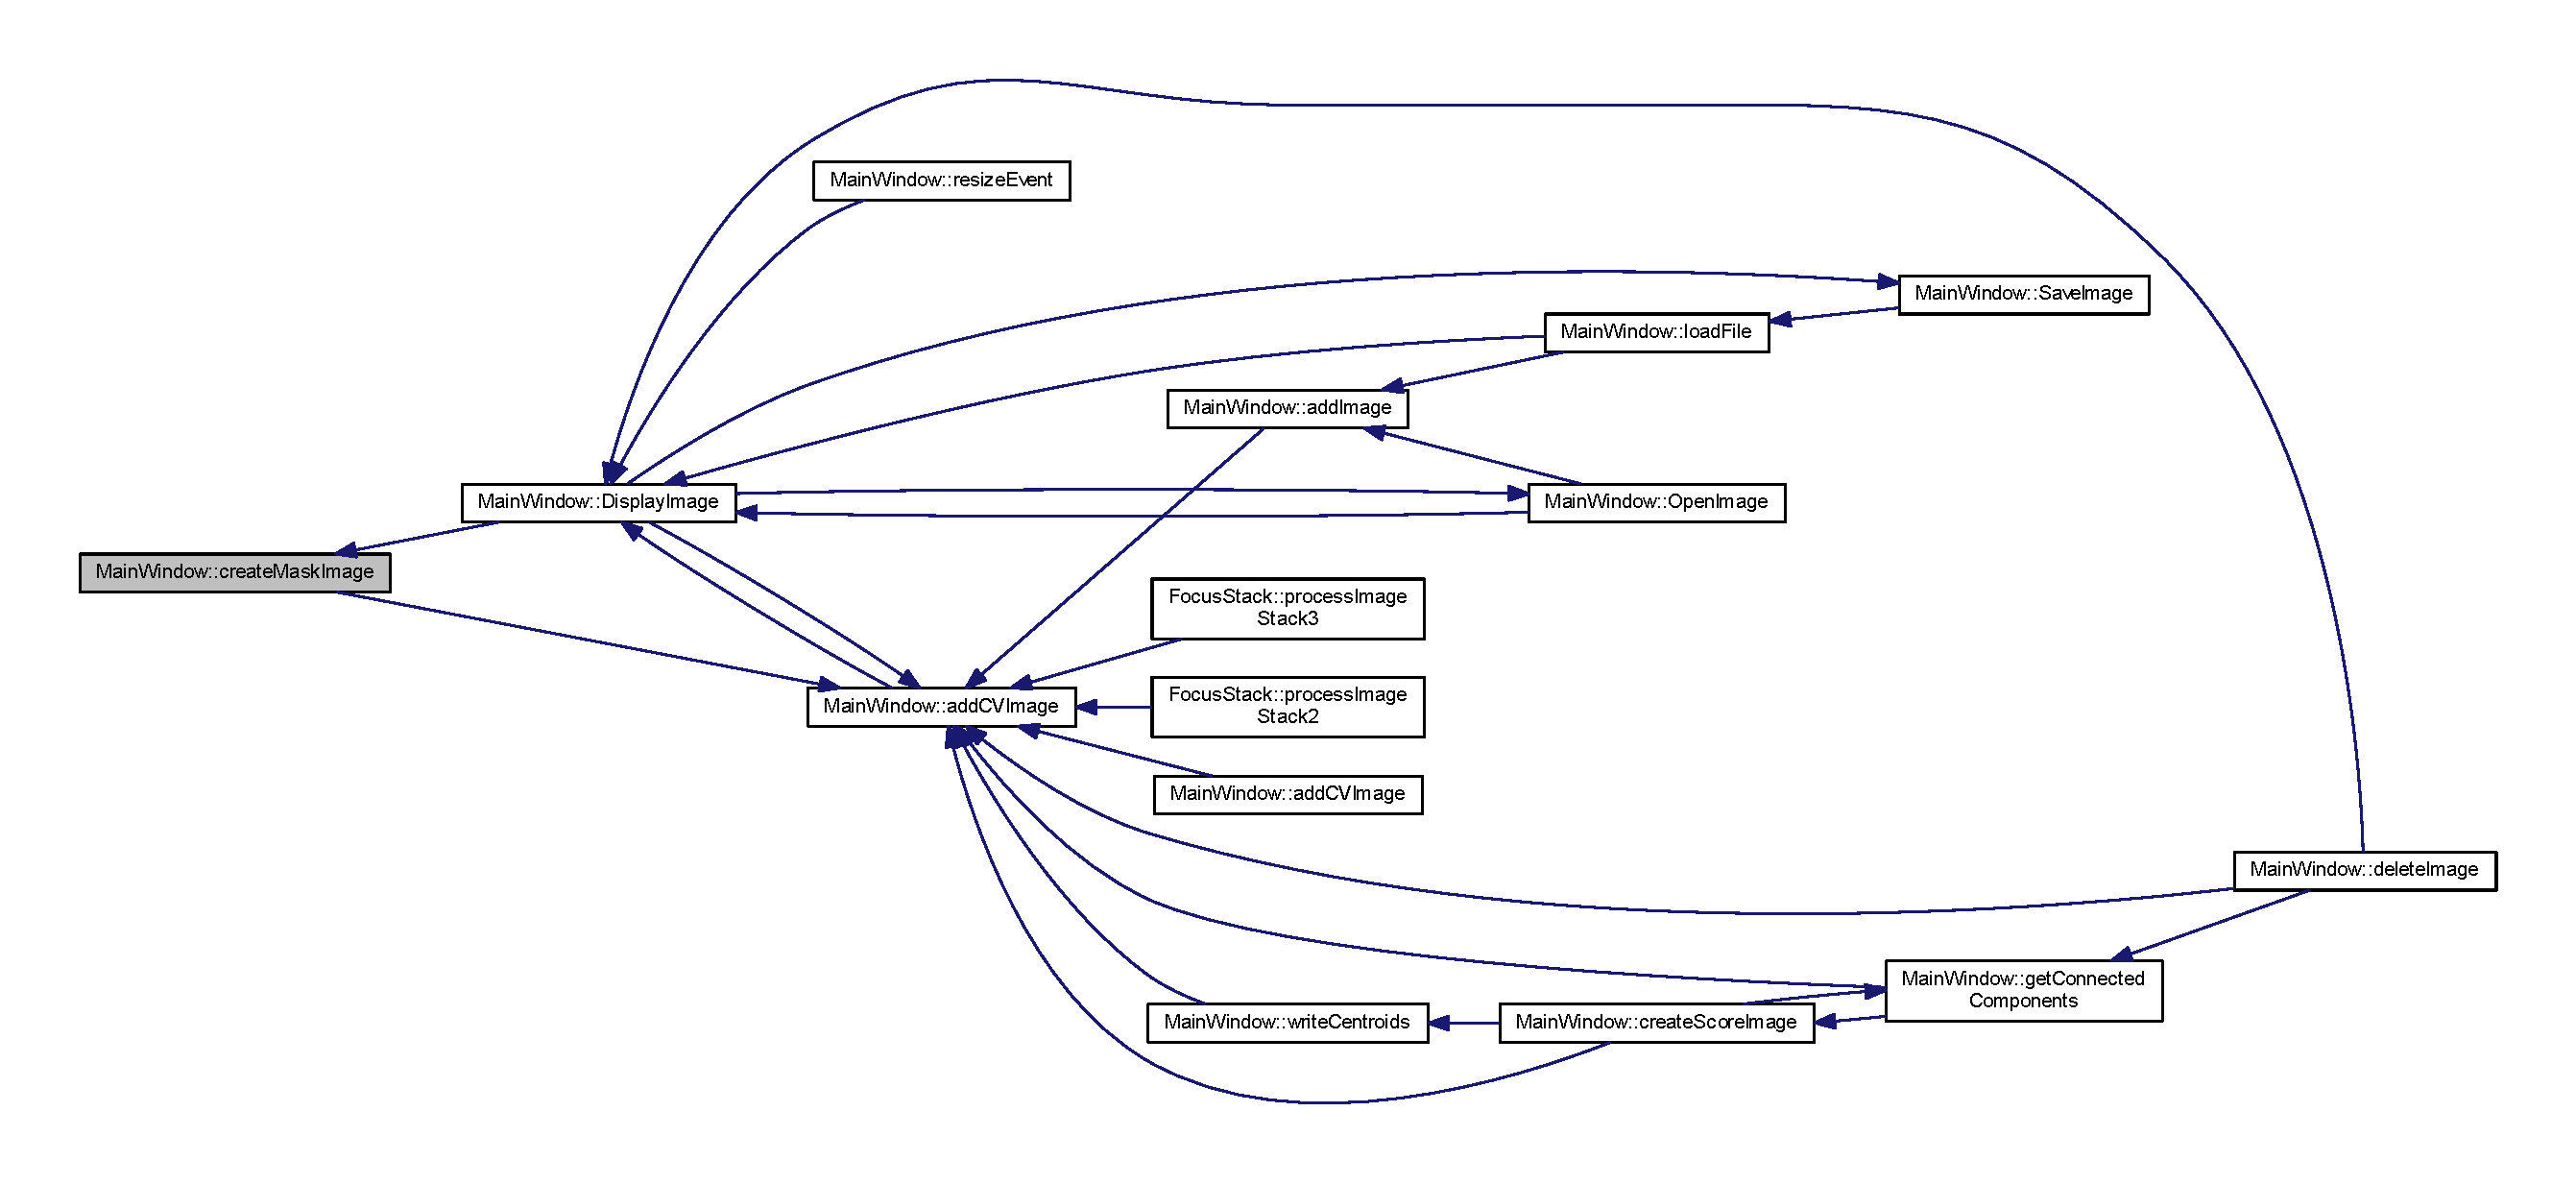
\includegraphics[width=350pt]{class_main_window_a92a40847027eaf2cf258c3a9f8da4c48_icgraph}
\end{center}
\end{figure}
\mbox{\Hypertarget{class_main_window_a8d87cd33d22ce614c9d7945264588e5f}\label{class_main_window_a8d87cd33d22ce614c9d7945264588e5f}} 
\index{Main\+Window@{Main\+Window}!create\+Score\+Image@{create\+Score\+Image}}
\index{create\+Score\+Image@{create\+Score\+Image}!Main\+Window@{Main\+Window}}
\subsubsection{\texorpdfstring{create\+Score\+Image()}{createScoreImage()}}
{\footnotesize\ttfamily cv\+::\+Mat Main\+Window\+::create\+Score\+Image (\begin{DoxyParamCaption}{ }\end{DoxyParamCaption})}

Slot to score image of possible targets found in the detection image

\begin{DoxyAuthor}{Author}
David Watts 
\end{DoxyAuthor}
\begin{DoxySince}{Since}
2017/03/17
\end{DoxySince}
Full\+Name \hyperlink{class_main_window_a8d87cd33d22ce614c9d7945264588e5f}{Main\+Window\+::create\+Score\+Image} Qualifier \begin{DoxyReturn}{Returns}
cv\+::\+Mat Access public 
\end{DoxyReturn}


Definition at line 2043 of file mainwindow.\+cpp.

Here is the call graph for this function\+:
\nopagebreak
\begin{figure}[H]
\begin{center}
\leavevmode
\includegraphics[width=350pt]{class_main_window_a8d87cd33d22ce614c9d7945264588e5f_cgraph}
\end{center}
\end{figure}
Here is the caller graph for this function\+:
\nopagebreak
\begin{figure}[H]
\begin{center}
\leavevmode
\includegraphics[width=350pt]{class_main_window_a8d87cd33d22ce614c9d7945264588e5f_icgraph}
\end{center}
\end{figure}
\mbox{\Hypertarget{class_main_window_ad0219fc878a0bc02403d00a16b7fc7ec}\label{class_main_window_ad0219fc878a0bc02403d00a16b7fc7ec}} 
\index{Main\+Window@{Main\+Window}!delete\+Image@{delete\+Image}}
\index{delete\+Image@{delete\+Image}!Main\+Window@{Main\+Window}}
\subsubsection{\texorpdfstring{delete\+Image()}{deleteImage()}}
{\footnotesize\ttfamily void Main\+Window\+::delete\+Image (\begin{DoxyParamCaption}\item[{int}]{index,  }\item[{bool}]{b\+Display = {\ttfamily true} }\end{DoxyParamCaption})}

removes image at array index

\begin{DoxyAuthor}{Author}
David Watts 
\end{DoxyAuthor}
\begin{DoxySince}{Since}
2017/03/07
\end{DoxySince}
Full\+Name \hyperlink{class_main_window_ad0219fc878a0bc02403d00a16b7fc7ec}{Main\+Window\+::delete\+Image} Qualifier 
\begin{DoxyParams}{Parameters}
{\em int} & index \\
\hline
\end{DoxyParams}
\begin{DoxyReturn}{Returns}
bool Access public 
\end{DoxyReturn}


Definition at line 1610 of file mainwindow.\+cpp.

Here is the call graph for this function\+:
\nopagebreak
\begin{figure}[H]
\begin{center}
\leavevmode
\includegraphics[width=350pt]{class_main_window_ad0219fc878a0bc02403d00a16b7fc7ec_cgraph}
\end{center}
\end{figure}
\mbox{\Hypertarget{class_main_window_a8e20e1254b179ca9ec054ec908d9cc43}\label{class_main_window_a8e20e1254b179ca9ec054ec908d9cc43}} 
\index{Main\+Window@{Main\+Window}!Display\+Image@{Display\+Image}}
\index{Display\+Image@{Display\+Image}!Main\+Window@{Main\+Window}}
\subsubsection{\texorpdfstring{Display\+Image}{DisplayImage}}
{\footnotesize\ttfamily void Main\+Window\+::\+Display\+Image (\begin{DoxyParamCaption}{ }\end{DoxyParamCaption})\hspace{0.3cm}{\ttfamily [slot]}}

Displays image in widget

\begin{DoxyAuthor}{Author}
David Watts 
\end{DoxyAuthor}
\begin{DoxySince}{Since}
2017/03/07
\end{DoxySince}
Full\+Name \hyperlink{class_main_window_a8e20e1254b179ca9ec054ec908d9cc43}{Main\+Window\+::\+Display\+Image} Qualifier \begin{DoxyReturn}{Returns}
void Access public 
\end{DoxyReturn}


Definition at line 1085 of file mainwindow.\+cpp.

Here is the call graph for this function\+:
\nopagebreak
\begin{figure}[H]
\begin{center}
\leavevmode
\includegraphics[width=350pt]{class_main_window_a8e20e1254b179ca9ec054ec908d9cc43_cgraph}
\end{center}
\end{figure}
Here is the caller graph for this function\+:
\nopagebreak
\begin{figure}[H]
\begin{center}
\leavevmode
\includegraphics[width=350pt]{class_main_window_a8e20e1254b179ca9ec054ec908d9cc43_icgraph}
\end{center}
\end{figure}
\mbox{\Hypertarget{class_main_window_ad68b6789cc86ef20cd7cedd6de8d4ed2}\label{class_main_window_ad68b6789cc86ef20cd7cedd6de8d4ed2}} 
\index{Main\+Window@{Main\+Window}!draw\+Centroids@{draw\+Centroids}}
\index{draw\+Centroids@{draw\+Centroids}!Main\+Window@{Main\+Window}}
\subsubsection{\texorpdfstring{draw\+Centroids()}{drawCentroids()}}
{\footnotesize\ttfamily void Main\+Window\+::draw\+Centroids (\begin{DoxyParamCaption}\item[{\hyperlink{classtargeter_image}{targeter\+Image} \&}]{tim,  }\item[{cv\+::\+Mat \&}]{drawimage }\end{DoxyParamCaption})}

Draws crosses at centroid positions of connected component regions on supplied cv\+::\+Mat image

\begin{DoxyAuthor}{Author}
David Watts 
\end{DoxyAuthor}
\begin{DoxySince}{Since}
2017/03/17
\end{DoxySince}
Full\+Name \hyperlink{class_main_window_ad68b6789cc86ef20cd7cedd6de8d4ed2}{Main\+Window\+::draw\+Centroids} Qualifier 
\begin{DoxyParams}{Parameters}
{\em \hyperlink{classtargeter_image}{targeter\+Image}} & \& tim \\
\hline
{\em cv\+::\+Mat} & \& drawimage \\
\hline
\end{DoxyParams}
\begin{DoxyReturn}{Returns}
void Access public 
\end{DoxyReturn}


Definition at line 2185 of file mainwindow.\+cpp.

Here is the call graph for this function\+:
\nopagebreak
\begin{figure}[H]
\begin{center}
\leavevmode
\includegraphics[width=350pt]{class_main_window_ad68b6789cc86ef20cd7cedd6de8d4ed2_cgraph}
\end{center}
\end{figure}
Here is the caller graph for this function\+:
\nopagebreak
\begin{figure}[H]
\begin{center}
\leavevmode
\includegraphics[width=350pt]{class_main_window_ad68b6789cc86ef20cd7cedd6de8d4ed2_icgraph}
\end{center}
\end{figure}
\mbox{\Hypertarget{class_main_window_a1e798fdae21c3294495ea7994df1887a}\label{class_main_window_a1e798fdae21c3294495ea7994df1887a}} 
\index{Main\+Window@{Main\+Window}!get\+Checked\+Images@{get\+Checked\+Images}}
\index{get\+Checked\+Images@{get\+Checked\+Images}!Main\+Window@{Main\+Window}}
\subsubsection{\texorpdfstring{get\+Checked\+Images()}{getCheckedImages()}}
{\footnotesize\ttfamily std\+::vector$<$ int $>$ Main\+Window\+::get\+Checked\+Images (\begin{DoxyParamCaption}{ }\end{DoxyParamCaption})}

Get vector of checked images in list

\begin{DoxyAuthor}{Author}
David Watts 
\end{DoxyAuthor}
\begin{DoxySince}{Since}
2017/03/07
\end{DoxySince}
Full\+Name \hyperlink{class_main_window_a1e798fdae21c3294495ea7994df1887a}{Main\+Window\+::get\+Checked\+Images} Qualifier \begin{DoxyReturn}{Returns}
Q\+Vector$<$int$>$ Access public 
\end{DoxyReturn}


Definition at line 952 of file mainwindow.\+cpp.

Here is the caller graph for this function\+:
\nopagebreak
\begin{figure}[H]
\begin{center}
\leavevmode
\includegraphics[width=350pt]{class_main_window_a1e798fdae21c3294495ea7994df1887a_icgraph}
\end{center}
\end{figure}
\mbox{\Hypertarget{class_main_window_a49cfabc6ef4845c5a9b5c9a92c9d4e2e}\label{class_main_window_a49cfabc6ef4845c5a9b5c9a92c9d4e2e}} 
\index{Main\+Window@{Main\+Window}!get\+Connected\+Components@{get\+Connected\+Components}}
\index{get\+Connected\+Components@{get\+Connected\+Components}!Main\+Window@{Main\+Window}}
\subsubsection{\texorpdfstring{get\+Connected\+Components()}{getConnectedComponents()}}
{\footnotesize\ttfamily \hyperlink{classtargeter_image}{targeter\+Image} Main\+Window\+::get\+Connected\+Components (\begin{DoxyParamCaption}\item[{cv\+::\+Mat \&}]{im }\end{DoxyParamCaption})}

Sets connected component image structure from binary image

\begin{DoxyAuthor}{Author}
David Watts 
\end{DoxyAuthor}
\begin{DoxySince}{Since}
2017/03/17
\end{DoxySince}
Full\+Name \hyperlink{class_main_window_a49cfabc6ef4845c5a9b5c9a92c9d4e2e}{Main\+Window\+::get\+Connected\+Components} Qualifier 
\begin{DoxyParams}{Parameters}
{\em cv\+::\+Mat} & \& im \\
\hline
\end{DoxyParams}
\begin{DoxyReturn}{Returns}
\hyperlink{classtargeter_image}{targeter\+Image}\& Access public 
\end{DoxyReturn}


Definition at line 1929 of file mainwindow.\+cpp.

Here is the call graph for this function\+:
\nopagebreak
\begin{figure}[H]
\begin{center}
\leavevmode
\includegraphics[width=350pt]{class_main_window_a49cfabc6ef4845c5a9b5c9a92c9d4e2e_cgraph}
\end{center}
\end{figure}
Here is the caller graph for this function\+:
\nopagebreak
\begin{figure}[H]
\begin{center}
\leavevmode
\includegraphics[width=350pt]{class_main_window_a49cfabc6ef4845c5a9b5c9a92c9d4e2e_icgraph}
\end{center}
\end{figure}
\mbox{\Hypertarget{class_main_window_a2734ce9308b5847a561f00b2fc9066aa}\label{class_main_window_a2734ce9308b5847a561f00b2fc9066aa}} 
\index{Main\+Window@{Main\+Window}!get\+Histogram@{get\+Histogram}}
\index{get\+Histogram@{get\+Histogram}!Main\+Window@{Main\+Window}}
\subsubsection{\texorpdfstring{get\+Histogram()}{getHistogram()}}
{\footnotesize\ttfamily cv\+::\+Mat Main\+Window\+::get\+Histogram (\begin{DoxyParamCaption}{ }\end{DoxyParamCaption})}

Gets image histogram

\begin{DoxyAuthor}{Author}
David Watts 
\end{DoxyAuthor}
\begin{DoxySince}{Since}
2017/03/17
\end{DoxySince}
Full\+Name \hyperlink{class_main_window_a2734ce9308b5847a561f00b2fc9066aa}{Main\+Window\+::get\+Histogram} Qualifier \begin{DoxyReturn}{Returns}
cv\+::\+Mat Access public 
\end{DoxyReturn}


Definition at line 522 of file mainwindow.\+cpp.

Here is the call graph for this function\+:
\nopagebreak
\begin{figure}[H]
\begin{center}
\leavevmode
\includegraphics[width=350pt]{class_main_window_a2734ce9308b5847a561f00b2fc9066aa_cgraph}
\end{center}
\end{figure}
Here is the caller graph for this function\+:
\nopagebreak
\begin{figure}[H]
\begin{center}
\leavevmode
\includegraphics[width=350pt]{class_main_window_a2734ce9308b5847a561f00b2fc9066aa_icgraph}
\end{center}
\end{figure}
\mbox{\Hypertarget{class_main_window_acc35ff9a0c04d62297e7fd219fa869e5}\label{class_main_window_acc35ff9a0c04d62297e7fd219fa869e5}} 
\index{Main\+Window@{Main\+Window}!get\+Valid\+Image\+Index@{get\+Valid\+Image\+Index}}
\index{get\+Valid\+Image\+Index@{get\+Valid\+Image\+Index}!Main\+Window@{Main\+Window}}
\subsubsection{\texorpdfstring{get\+Valid\+Image\+Index()}{getValidImageIndex()}}
{\footnotesize\ttfamily int Main\+Window\+::get\+Valid\+Image\+Index (\begin{DoxyParamCaption}{ }\end{DoxyParamCaption})}

Gets valid image array index, if current image index is invalid then function returns last valid index

\begin{DoxyAuthor}{Author}
David Watts 
\end{DoxyAuthor}
\begin{DoxySince}{Since}
2017/03/07
\end{DoxySince}
Full\+Name \hyperlink{class_main_window_acc35ff9a0c04d62297e7fd219fa869e5}{Main\+Window\+::get\+Valid\+Image\+Index} Qualifier \begin{DoxyReturn}{Returns}
int Access public 
\end{DoxyReturn}


Definition at line 1047 of file mainwindow.\+cpp.

Here is the call graph for this function\+:
\nopagebreak
\begin{figure}[H]
\begin{center}
\leavevmode
\includegraphics[width=350pt]{class_main_window_acc35ff9a0c04d62297e7fd219fa869e5_cgraph}
\end{center}
\end{figure}
Here is the caller graph for this function\+:
\nopagebreak
\begin{figure}[H]
\begin{center}
\leavevmode
\includegraphics[width=350pt]{class_main_window_acc35ff9a0c04d62297e7fd219fa869e5_icgraph}
\end{center}
\end{figure}
\mbox{\Hypertarget{class_main_window_aa08469ed5c8396e60fa44bae6530bcf1}\label{class_main_window_aa08469ed5c8396e60fa44bae6530bcf1}} 
\index{Main\+Window@{Main\+Window}!load\+File@{load\+File}}
\index{load\+File@{load\+File}!Main\+Window@{Main\+Window}}
\subsubsection{\texorpdfstring{load\+File()}{loadFile()}}
{\footnotesize\ttfamily void Main\+Window\+::load\+File (\begin{DoxyParamCaption}\item[{const Q\+String \&}]{file\+Name }\end{DoxyParamCaption})}

loads image file

\begin{DoxyAuthor}{Author}
David Watts 
\end{DoxyAuthor}
\begin{DoxySince}{Since}
2017/03/07
\end{DoxySince}
Full\+Name \hyperlink{class_main_window_aa08469ed5c8396e60fa44bae6530bcf1}{Main\+Window\+::load\+File} Qualifier 
\begin{DoxyParams}{Parameters}
{\em const} & Q\+String \& file\+Name \\
\hline
\end{DoxyParams}
\begin{DoxyReturn}{Returns}
void Access public 
\end{DoxyReturn}


Definition at line 396 of file mainwindow.\+cpp.

Here is the call graph for this function\+:
\nopagebreak
\begin{figure}[H]
\begin{center}
\leavevmode
\includegraphics[width=350pt]{class_main_window_aa08469ed5c8396e60fa44bae6530bcf1_cgraph}
\end{center}
\end{figure}
Here is the caller graph for this function\+:
\nopagebreak
\begin{figure}[H]
\begin{center}
\leavevmode
\includegraphics[width=350pt]{class_main_window_aa08469ed5c8396e60fa44bae6530bcf1_icgraph}
\end{center}
\end{figure}
\mbox{\Hypertarget{class_main_window_acea9cebdcf70bf45107baa0789e732bf}\label{class_main_window_acea9cebdcf70bf45107baa0789e732bf}} 
\index{Main\+Window@{Main\+Window}!Open\+Image@{Open\+Image}}
\index{Open\+Image@{Open\+Image}!Main\+Window@{Main\+Window}}
\subsubsection{\texorpdfstring{Open\+Image()}{OpenImage()}}
{\footnotesize\ttfamily void Main\+Window\+::\+Open\+Image (\begin{DoxyParamCaption}{ }\end{DoxyParamCaption})}

Handles Opening of image from file open dialog

\begin{DoxyAuthor}{Author}
David Watts 
\end{DoxyAuthor}
\begin{DoxySince}{Since}
2017/03/07
\end{DoxySince}
Full\+Name \hyperlink{class_main_window_acea9cebdcf70bf45107baa0789e732bf}{Main\+Window\+::\+Open\+Image} Qualifier \begin{DoxyReturn}{Returns}
void Access public 
\end{DoxyReturn}


Definition at line 805 of file mainwindow.\+cpp.

Here is the call graph for this function\+:
\nopagebreak
\begin{figure}[H]
\begin{center}
\leavevmode
\includegraphics[width=350pt]{class_main_window_acea9cebdcf70bf45107baa0789e732bf_cgraph}
\end{center}
\end{figure}
Here is the caller graph for this function\+:
\nopagebreak
\begin{figure}[H]
\begin{center}
\leavevmode
\includegraphics[width=350pt]{class_main_window_acea9cebdcf70bf45107baa0789e732bf_icgraph}
\end{center}
\end{figure}
\mbox{\Hypertarget{class_main_window_ae12f8f63791595567b6250f8bb002bda}\label{class_main_window_ae12f8f63791595567b6250f8bb002bda}} 
\index{Main\+Window@{Main\+Window}!resize\+Event@{resize\+Event}}
\index{resize\+Event@{resize\+Event}!Main\+Window@{Main\+Window}}
\subsubsection{\texorpdfstring{resize\+Event()}{resizeEvent()}}
{\footnotesize\ttfamily void Main\+Window\+::resize\+Event (\begin{DoxyParamCaption}\item[{Q\+Resize\+Event $\ast$}]{event }\end{DoxyParamCaption})}

manage image redrawing when window resized

\begin{DoxyAuthor}{Author}
David Watts 
\end{DoxyAuthor}
\begin{DoxySince}{Since}
2017/03/07
\end{DoxySince}
Full\+Name \hyperlink{class_main_window_ae12f8f63791595567b6250f8bb002bda}{Main\+Window\+::resize\+Event} Qualifier 
\begin{DoxyParams}{Parameters}
{\em Q\+Resize\+Event} & $\ast$ event \\
\hline
\end{DoxyParams}
\begin{DoxyReturn}{Returns}
void Access public 
\end{DoxyReturn}


Definition at line 1022 of file mainwindow.\+cpp.

Here is the call graph for this function\+:
\nopagebreak
\begin{figure}[H]
\begin{center}
\leavevmode
\includegraphics[width=350pt]{class_main_window_ae12f8f63791595567b6250f8bb002bda_cgraph}
\end{center}
\end{figure}
\mbox{\Hypertarget{class_main_window_aa816921e6ce14f558ada5c73c8a5ef20}\label{class_main_window_aa816921e6ce14f558ada5c73c8a5ef20}} 
\index{Main\+Window@{Main\+Window}!Save\+Image@{Save\+Image}}
\index{Save\+Image@{Save\+Image}!Main\+Window@{Main\+Window}}
\subsubsection{\texorpdfstring{Save\+Image()}{SaveImage()}}
{\footnotesize\ttfamily void Main\+Window\+::\+Save\+Image (\begin{DoxyParamCaption}{ }\end{DoxyParamCaption})}

Saves current image to file

\begin{DoxyAuthor}{Author}
David Watts 
\end{DoxyAuthor}
\begin{DoxySince}{Since}
2017/03/07
\end{DoxySince}
Full\+Name \hyperlink{class_main_window_aa816921e6ce14f558ada5c73c8a5ef20}{Main\+Window\+::\+Save\+Image} Qualifier \begin{DoxyReturn}{Returns}
void Access public 
\end{DoxyReturn}


Definition at line 340 of file mainwindow.\+cpp.

Here is the call graph for this function\+:
\nopagebreak
\begin{figure}[H]
\begin{center}
\leavevmode
\includegraphics[width=350pt]{class_main_window_aa816921e6ce14f558ada5c73c8a5ef20_cgraph}
\end{center}
\end{figure}
Here is the caller graph for this function\+:
\nopagebreak
\begin{figure}[H]
\begin{center}
\leavevmode
\includegraphics[width=350pt]{class_main_window_aa816921e6ce14f558ada5c73c8a5ef20_icgraph}
\end{center}
\end{figure}
\mbox{\Hypertarget{class_main_window_a5e130e8122dbab96f931a7ecc41086d3}\label{class_main_window_a5e130e8122dbab96f931a7ecc41086d3}} 
\index{Main\+Window@{Main\+Window}!set\+Histogram\+Image@{set\+Histogram\+Image}}
\index{set\+Histogram\+Image@{set\+Histogram\+Image}!Main\+Window@{Main\+Window}}
\subsubsection{\texorpdfstring{set\+Histogram\+Image()}{setHistogramImage()}}
{\footnotesize\ttfamily void Main\+Window\+::set\+Histogram\+Image (\begin{DoxyParamCaption}{ }\end{DoxyParamCaption})}

Sets image histogram in settings dialog

\begin{DoxyAuthor}{Author}
David Watts 
\end{DoxyAuthor}
\begin{DoxySince}{Since}
2017/03/07
\end{DoxySince}
Full\+Name \hyperlink{class_main_window_a5e130e8122dbab96f931a7ecc41086d3}{Main\+Window\+::set\+Histogram\+Image} Qualifier \begin{DoxyReturn}{Returns}
void Access public 
\end{DoxyReturn}


Definition at line 496 of file mainwindow.\+cpp.

Here is the call graph for this function\+:
\nopagebreak
\begin{figure}[H]
\begin{center}
\leavevmode
\includegraphics[width=350pt]{class_main_window_a5e130e8122dbab96f931a7ecc41086d3_cgraph}
\end{center}
\end{figure}
Here is the caller graph for this function\+:
\nopagebreak
\begin{figure}[H]
\begin{center}
\leavevmode
\includegraphics[width=350pt]{class_main_window_a5e130e8122dbab96f931a7ecc41086d3_icgraph}
\end{center}
\end{figure}
\mbox{\Hypertarget{class_main_window_a280d25148ac076ca817d411372584ae5}\label{class_main_window_a280d25148ac076ca817d411372584ae5}} 
\index{Main\+Window@{Main\+Window}!show\+Message@{show\+Message}}
\index{show\+Message@{show\+Message}!Main\+Window@{Main\+Window}}
\subsubsection{\texorpdfstring{show\+Message()}{showMessage()}\hspace{0.1cm}{\footnotesize\ttfamily [1/2]}}
{\footnotesize\ttfamily void Main\+Window\+::show\+Message (\begin{DoxyParamCaption}\item[{image\+Type\+::image\+Type}]{type,  }\item[{Q\+Message\+Box\+::\+Icon}]{icn = {\ttfamily QMessageBox\+:\+:Warning} }\end{DoxyParamCaption})}

Displays message box depending on image type

\begin{DoxyAuthor}{Author}
David Watts 
\end{DoxyAuthor}
\begin{DoxySince}{Since}
2017/03/17
\end{DoxySince}
Full\+Name \hyperlink{class_main_window_a280d25148ac076ca817d411372584ae5}{Main\+Window\+::show\+Message} Qualifier 
\begin{DoxyParams}{Parameters}
{\em image\+Type\+::image\+Type} & type \\
\hline
{\em Q\+Message\+Box\+::\+Icon} & icn \\
\hline
\end{DoxyParams}
\begin{DoxyReturn}{Returns}
void Access public 
\end{DoxyReturn}


Definition at line 437 of file mainwindow.\+cpp.

Here is the caller graph for this function\+:
\nopagebreak
\begin{figure}[H]
\begin{center}
\leavevmode
\includegraphics[width=350pt]{class_main_window_a280d25148ac076ca817d411372584ae5_icgraph}
\end{center}
\end{figure}
\mbox{\Hypertarget{class_main_window_aebde68c58d77b71d20fa6816b751356e}\label{class_main_window_aebde68c58d77b71d20fa6816b751356e}} 
\index{Main\+Window@{Main\+Window}!show\+Message@{show\+Message}}
\index{show\+Message@{show\+Message}!Main\+Window@{Main\+Window}}
\subsubsection{\texorpdfstring{show\+Message()}{showMessage()}\hspace{0.1cm}{\footnotesize\ttfamily [2/2]}}
{\footnotesize\ttfamily void Main\+Window\+::show\+Message (\begin{DoxyParamCaption}\item[{Q\+String}]{message,  }\item[{Q\+Message\+Box\+::\+Icon}]{icn = {\ttfamily QMessageBox\+:\+:Warning} }\end{DoxyParamCaption})}

Displays message box

\begin{DoxyAuthor}{Author}
David Watts 
\end{DoxyAuthor}
\begin{DoxySince}{Since}
2017/03/17
\end{DoxySince}
Full\+Name \hyperlink{class_main_window_a280d25148ac076ca817d411372584ae5}{Main\+Window\+::show\+Message} Qualifier 
\begin{DoxyParams}{Parameters}
{\em Q\+String} & message \\
\hline
{\em Q\+Message\+Box\+::\+Icon} & icn \\
\hline
\end{DoxyParams}
\begin{DoxyReturn}{Returns}
void Access public 
\end{DoxyReturn}


Definition at line 473 of file mainwindow.\+cpp.

\mbox{\Hypertarget{class_main_window_a171b0591a4f66b4b16a33d4af5c35465}\label{class_main_window_a171b0591a4f66b4b16a33d4af5c35465}} 
\index{Main\+Window@{Main\+Window}!update\+Image\+Type@{update\+Image\+Type}}
\index{update\+Image\+Type@{update\+Image\+Type}!Main\+Window@{Main\+Window}}
\subsubsection{\texorpdfstring{update\+Image\+Type()}{updateImageType()}}
{\footnotesize\ttfamily void Main\+Window\+::update\+Image\+Type (\begin{DoxyParamCaption}\item[{int}]{ind,  }\item[{image\+Type\+::image\+Type}]{type }\end{DoxyParamCaption})}

sets type of image

\begin{DoxyAuthor}{Author}
David Watts 
\end{DoxyAuthor}
\begin{DoxySince}{Since}
2017/03/14
\end{DoxySince}
Full\+Name \hyperlink{class_main_window_a171b0591a4f66b4b16a33d4af5c35465}{Main\+Window\+::update\+Image\+Type} Qualifier 
\begin{DoxyParams}{Parameters}
{\em int} & ind \\
\hline
{\em image\+Type\+::image\+Type} & type \\
\hline
\end{DoxyParams}
\begin{DoxyReturn}{Returns}
void Access public 
\end{DoxyReturn}


Definition at line 1545 of file mainwindow.\+cpp.

Here is the call graph for this function\+:
\nopagebreak
\begin{figure}[H]
\begin{center}
\leavevmode
\includegraphics[width=350pt]{class_main_window_a171b0591a4f66b4b16a33d4af5c35465_cgraph}
\end{center}
\end{figure}
Here is the caller graph for this function\+:
\nopagebreak
\begin{figure}[H]
\begin{center}
\leavevmode
\includegraphics[width=350pt]{class_main_window_a171b0591a4f66b4b16a33d4af5c35465_icgraph}
\end{center}
\end{figure}
\mbox{\Hypertarget{class_main_window_a89dfa31ef44692bb1d7307f0c35838c0}\label{class_main_window_a89dfa31ef44692bb1d7307f0c35838c0}} 
\index{Main\+Window@{Main\+Window}!update\+Thumbs@{update\+Thumbs}}
\index{update\+Thumbs@{update\+Thumbs}!Main\+Window@{Main\+Window}}
\subsubsection{\texorpdfstring{update\+Thumbs()}{updateThumbs()}}
{\footnotesize\ttfamily void Main\+Window\+::update\+Thumbs (\begin{DoxyParamCaption}\item[{int}]{index = {\ttfamily -\/1} }\end{DoxyParamCaption})}

update labels of thumbnail images

\begin{DoxyAuthor}{Author}
David Watts 
\end{DoxyAuthor}
\begin{DoxySince}{Since}
2017/03/07
\end{DoxySince}
Full\+Name \hyperlink{class_main_window_a89dfa31ef44692bb1d7307f0c35838c0}{Main\+Window\+::update\+Thumbs} Qualifier 
\begin{DoxyParams}{Parameters}
{\em int} & index \\
\hline
\end{DoxyParams}
\begin{DoxyReturn}{Returns}
void Access public 
\end{DoxyReturn}


Definition at line 703 of file mainwindow.\+cpp.

Here is the caller graph for this function\+:
\nopagebreak
\begin{figure}[H]
\begin{center}
\leavevmode
\includegraphics[width=350pt]{class_main_window_a89dfa31ef44692bb1d7307f0c35838c0_icgraph}
\end{center}
\end{figure}
\mbox{\Hypertarget{class_main_window_aa137f4371bae807873da7862f4102521}\label{class_main_window_aa137f4371bae807873da7862f4102521}} 
\index{Main\+Window@{Main\+Window}!write\+Centroids@{write\+Centroids}}
\index{write\+Centroids@{write\+Centroids}!Main\+Window@{Main\+Window}}
\subsubsection{\texorpdfstring{write\+Centroids()}{writeCentroids()}}
{\footnotesize\ttfamily void Main\+Window\+::write\+Centroids (\begin{DoxyParamCaption}\item[{\hyperlink{classtargeter_image}{targeter\+Image} \&}]{tim,  }\item[{Q\+File \&}]{xml\+File }\end{DoxyParamCaption})}

Writes X\+ML of target locations in image

\begin{DoxyAuthor}{Author}
David Watts 
\end{DoxyAuthor}
\begin{DoxySince}{Since}
2017/03/17
\end{DoxySince}
Full\+Name \hyperlink{class_main_window_aa137f4371bae807873da7862f4102521}{Main\+Window\+::write\+Centroids} Qualifier 
\begin{DoxyParams}{Parameters}
{\em \hyperlink{classtargeter_image}{targeter\+Image}} & \& tim \\
\hline
{\em Q\+File} & \& xml\+File \\
\hline
\end{DoxyParams}
\begin{DoxyReturn}{Returns}
void Access public 
\end{DoxyReturn}


Definition at line 2221 of file mainwindow.\+cpp.

Here is the call graph for this function\+:
\nopagebreak
\begin{figure}[H]
\begin{center}
\leavevmode
\includegraphics[width=350pt]{class_main_window_aa137f4371bae807873da7862f4102521_cgraph}
\end{center}
\end{figure}
Here is the caller graph for this function\+:
\nopagebreak
\begin{figure}[H]
\begin{center}
\leavevmode
\includegraphics[width=350pt]{class_main_window_aa137f4371bae807873da7862f4102521_icgraph}
\end{center}
\end{figure}


The documentation for this class was generated from the following files\+:\begin{DoxyCompactItemize}
\item 
H\+:/\+Code\+Projects/\+Q\+T\+Projects/\+Targeter-\/msvc/mainwindow.\+h\item 
H\+:/\+Code\+Projects/\+Q\+T\+Projects/\+Targeter-\/msvc/mainwindow.\+cpp\end{DoxyCompactItemize}

\hypertarget{class_ui_1_1_main_window}{}\section{Ui\+:\+:Main\+Window Class Reference}
\label{class_ui_1_1_main_window}\index{Ui\+::\+Main\+Window@{Ui\+::\+Main\+Window}}


Inheritance diagram for Ui\+:\+:Main\+Window\+:
\nopagebreak
\begin{figure}[H]
\begin{center}
\leavevmode
\includegraphics[height=550pt]{class_ui_1_1_main_window__inherit__graph}
\end{center}
\end{figure}


Collaboration diagram for Ui\+:\+:Main\+Window\+:
\nopagebreak
\begin{figure}[H]
\begin{center}
\leavevmode
\includegraphics[height=550pt]{class_ui_1_1_main_window__coll__graph}
\end{center}
\end{figure}
\subsection*{Additional Inherited Members}


\subsection{Detailed Description}


Definition at line 567 of file ui\+\_\+mainwindow.\+h.



The documentation for this class was generated from the following file\+:\begin{DoxyCompactItemize}
\item 
H\+:/\+Code\+Projects/\+Q\+T\+Projects/\+Targeter-\/msvc/\+Generated\+Files/ui\+\_\+mainwindow.\+h\end{DoxyCompactItemize}

\hypertarget{class_merge_settings_dialog}{}\section{Merge\+Settings\+Dialog Class Reference}
\label{class_merge_settings_dialog}\index{Merge\+Settings\+Dialog@{Merge\+Settings\+Dialog}}


Inheritance diagram for Merge\+Settings\+Dialog\+:
\nopagebreak
\begin{figure}[H]
\begin{center}
\leavevmode
\includegraphics[width=208pt]{class_merge_settings_dialog__inherit__graph}
\end{center}
\end{figure}


Collaboration diagram for Merge\+Settings\+Dialog\+:
\nopagebreak
\begin{figure}[H]
\begin{center}
\leavevmode
\includegraphics[width=208pt]{class_merge_settings_dialog__coll__graph}
\end{center}
\end{figure}
\subsection*{Public Member Functions}
\begin{DoxyCompactItemize}
\item 
\mbox{\Hypertarget{class_merge_settings_dialog_ab334a7e18beccbb9dcb385dfc3d74ba6}\label{class_merge_settings_dialog_ab334a7e18beccbb9dcb385dfc3d74ba6}} 
{\bfseries Merge\+Settings\+Dialog} (Q\+Widget $\ast$parent=0)
\end{DoxyCompactItemize}


\subsection{Detailed Description}


Definition at line 10 of file mergesettingsdialog.\+h.



The documentation for this class was generated from the following files\+:\begin{DoxyCompactItemize}
\item 
H\+:/\+Code\+Projects/\+Q\+T\+Projects/\+Targeter-\/msvc/mergesettingsdialog.\+h\item 
H\+:/\+Code\+Projects/\+Q\+T\+Projects/\+Targeter-\/msvc/mergesettingsdialog.\+cpp\end{DoxyCompactItemize}

\hypertarget{class_open_c_vtrilateral_filter}{}\section{Open\+C\+Vtrilateral\+Filter Class Reference}
\label{class_open_c_vtrilateral_filter}\index{Open\+C\+Vtrilateral\+Filter@{Open\+C\+Vtrilateral\+Filter}}


Collaboration diagram for Open\+C\+Vtrilateral\+Filter\+:
\nopagebreak
\begin{figure}[H]
\begin{center}
\leavevmode
\includegraphics[width=211pt]{class_open_c_vtrilateral_filter__coll__graph}
\end{center}
\end{figure}
\subsection*{Public Types}
\begin{DoxyCompactItemize}
\item 
\mbox{\Hypertarget{class_open_c_vtrilateral_filter_a7d552e7b9918da0721e5c91638ef19ca}\label{class_open_c_vtrilateral_filter_a7d552e7b9918da0721e5c91638ef19ca}} 
enum \{ {\bfseries T\+Y\+P\+E\+\_\+\+L\+UT}, 
{\bfseries T\+Y\+P\+E\+\_\+\+F\+A\+ST}
 \}
\end{DoxyCompactItemize}
\subsection*{Public Member Functions}
\begin{DoxyCompactItemize}
\item 
\mbox{\Hypertarget{class_open_c_vtrilateral_filter_a01d5a2f9a2a8ae76906e1349f739a7bf}\label{class_open_c_vtrilateral_filter_a01d5a2f9a2a8ae76906e1349f739a7bf}} 
bool {\bfseries trilateral\+Filter} (cv\+::\+Mat \&input, cv\+::\+Mat \&output, const float sigmaC, const float epsilon, const int filter\+Type=T\+Y\+P\+E\+\_\+\+F\+A\+ST)
\item 
\mbox{\Hypertarget{class_open_c_vtrilateral_filter_ae1c2335bae77ec838b302dbfc41bd308}\label{class_open_c_vtrilateral_filter_ae1c2335bae77ec838b302dbfc41bd308}} 
cv\+::\+Mat {\bfseries trilateral\+Filter} (cv\+::\+Mat \&input, const float sigmaC, const float epsilon, const int filter\+Type=T\+Y\+P\+E\+\_\+\+F\+A\+ST)
\end{DoxyCompactItemize}


\subsection{Detailed Description}


Definition at line 10 of file open\+C\+Vtrilateral\+Filter.\+h.



The documentation for this class was generated from the following files\+:\begin{DoxyCompactItemize}
\item 
H\+:/\+Code\+Projects/\+Q\+T\+Projects/\+Targeter-\/msvc/open\+C\+Vtrilateral\+Filter.\+h\item 
H\+:/\+Code\+Projects/\+Q\+T\+Projects/\+Targeter-\/msvc/open\+C\+Vtrilateral\+Filter.\+cpp\end{DoxyCompactItemize}

\hypertarget{class_paint_q_label}{}\section{Paint\+Q\+Label Class Reference}
\label{class_paint_q_label}\index{Paint\+Q\+Label@{Paint\+Q\+Label}}


{\ttfamily \#include $<$paintqlabel.\+h$>$}



Inheritance diagram for Paint\+Q\+Label\+:
\nopagebreak
\begin{figure}[H]
\begin{center}
\leavevmode
\includegraphics[height=550pt]{class_paint_q_label__inherit__graph}
\end{center}
\end{figure}


Collaboration diagram for Paint\+Q\+Label\+:
\nopagebreak
\begin{figure}[H]
\begin{center}
\leavevmode
\includegraphics[height=550pt]{class_paint_q_label__coll__graph}
\end{center}
\end{figure}
\subsection*{Signals}
\begin{DoxyCompactItemize}
\item 
\mbox{\Hypertarget{class_paint_q_label_aef10b2d14a17cf5b838106d076fdfce4}\label{class_paint_q_label_aef10b2d14a17cf5b838106d076fdfce4}} 
void {\bfseries disable\+Pan\+Button} ()
\item 
\mbox{\Hypertarget{class_paint_q_label_a0aabd575fa4e3774689bbc0aafdc6fdb}\label{class_paint_q_label_a0aabd575fa4e3774689bbc0aafdc6fdb}} 
void {\bfseries set\+Target\+Area} (\hyperlink{structdrawing_shape}{drawing\+Shape} shape)
\item 
\mbox{\Hypertarget{class_paint_q_label_a84be2f2ab4315ae3d0d128c648d9933b}\label{class_paint_q_label_a84be2f2ab4315ae3d0d128c648d9933b}} 
void {\bfseries unset\+Drawing\+Buttons} ()
\end{DoxyCompactItemize}
\subsection*{Public Member Functions}
\begin{DoxyCompactItemize}
\item 
\hyperlink{class_paint_q_label_a079e85cd5d1ec31f20f3c0bb8b510ec2}{Paint\+Q\+Label} (Q\+Widget $\ast$parent=0)
\item 
\hyperlink{class_paint_q_label_a837d8485a5da3e3fc87a30a4ada47cf2}{$\sim$\+Paint\+Q\+Label} ()
\item 
void \hyperlink{class_paint_q_label_abe77c4ddb9e176c54374718d1e782af0}{display\+Rect} (Q\+Rect r)
\item 
void \hyperlink{class_paint_q_label_a58a4d1f0765a00967529fcbb9cecbc91}{get\+Display\+Rect} ()
\item 
void \hyperlink{class_paint_q_label_a18ac8d49bd128e0ce565b588a6e8b66a}{set\+Image} (Q\+Image im)
\item 
void \hyperlink{class_paint_q_label_a30afcb97e84548909b882e0514111e03}{zoom\+To\+Point} (Q\+Point window\+Click, int zoom\+Amount)
\item 
void \hyperlink{class_paint_q_label_a332bf0f6137c8613fbdeac4bd0c1516e}{get\+Polygon\+Rect} ()
\item 
void \hyperlink{class_paint_q_label_a15478ad03c1c6254c3474ab8deb0428f}{set\+Drawing\+Mode} (drawing\+Mode\+::drawing\+Mode mode)
\item 
void \hyperlink{class_paint_q_label_a9f76a4b2851a0906aee6738c91c76969}{set\+Pan\+Mode} (bool b\+Checked)
\item 
bool \hyperlink{class_paint_q_label_aa8b3fe000a0123047ef6b2c884db979a}{check\+For\+Polygon\+Close} (Q\+Point mp)
\item 
void \hyperlink{class_paint_q_label_a76f7bb92d5971c324ff0998babd5a70f}{start\+Panning} (drawing\+Mode\+::drawing\+Mode mode, Q\+Point pos)
\item 
bool \hyperlink{class_paint_q_label_a2ba7f833ed473795ad0e9f1ccb0f29b3}{in\+Ellipse} (Q\+Rect r, Q\+Point p)
\item 
bool \hyperlink{class_paint_q_label_aa01fed3a13d42241b4769d14290a85e6}{in\+Rect} (Q\+Rect r, Q\+Point p)
\item 
bool \hyperlink{class_paint_q_label_af6562b147730457b828f0c776ff001e6}{in\+Poly} (Q\+Vector$<$ Q\+Point $>$ verts, Q\+Point p)
\item 
void \hyperlink{class_paint_q_label_a56784c6095f3ff7938ccc1c76feb7ad6}{delete\+Selected\+Drawing\+Object} ()
\item 
void \hyperlink{class_paint_q_label_a409e0869a3115968f025878ad49d9883}{get\+Target\+Image} ()
\item 
void \hyperlink{class_paint_q_label_aeac060e87e6671f65fb3a5ff4e3f15f4}{reset\+Drawing\+Objects} ()
\end{DoxyCompactItemize}
\subsection*{Public Attributes}
\begin{DoxyCompactItemize}
\item 
\mbox{\Hypertarget{class_paint_q_label_a2f14ccc35abc58b1b5f675def203f1a5}\label{class_paint_q_label_a2f14ccc35abc58b1b5f675def203f1a5}} 
int {\bfseries m\+\_\+scale}
\item 
\mbox{\Hypertarget{class_paint_q_label_a82a12e67b0c4d0916736d6ab686b5274}\label{class_paint_q_label_a82a12e67b0c4d0916736d6ab686b5274}} 
Q\+Rect {\bfseries m\+\_\+display\+Rect}
\item 
\mbox{\Hypertarget{class_paint_q_label_a5c521eb8af035302726ceb30d3865325}\label{class_paint_q_label_a5c521eb8af035302726ceb30d3865325}} 
Q\+Rect {\bfseries m\+\_\+image\+Rect}
\item 
\mbox{\Hypertarget{class_paint_q_label_aa317523c692351ba275ab8d961877332}\label{class_paint_q_label_aa317523c692351ba275ab8d961877332}} 
double {\bfseries m\+\_\+aspect\+Ratio}
\item 
\mbox{\Hypertarget{class_paint_q_label_a98346a1eb5b6dd9fe5b07e293142b63f}\label{class_paint_q_label_a98346a1eb5b6dd9fe5b07e293142b63f}} 
Q\+Image {\bfseries m\+\_\+\+Image}
\item 
\mbox{\Hypertarget{class_paint_q_label_a2f5060008173c178f3bff4718b668a22}\label{class_paint_q_label_a2f5060008173c178f3bff4718b668a22}} 
Q\+Vector$<$ Q\+Point $>$ {\bfseries m\+\_\+\+Polygon\+Points}
\item 
\mbox{\Hypertarget{class_paint_q_label_ad0d70f6b959cce938e2015413945353c}\label{class_paint_q_label_ad0d70f6b959cce938e2015413945353c}} 
bool {\bfseries m\+\_\+b\+Loop\+Closed}
\item 
\mbox{\Hypertarget{class_paint_q_label_ab98fc5e0aafa68de5b0f0a2775c0c346}\label{class_paint_q_label_ab98fc5e0aafa68de5b0f0a2775c0c346}} 
Q\+Rect {\bfseries m\+\_\+bounding\+Polygon}
\item 
\mbox{\Hypertarget{class_paint_q_label_a82c7a19109e2e455c1af992a312c5809}\label{class_paint_q_label_a82c7a19109e2e455c1af992a312c5809}} 
Q\+Rect {\bfseries m\+\_\+bounding\+Rectangle}
\item 
\mbox{\Hypertarget{class_paint_q_label_a463e17ba1635d2d23ba5fa35d0927e84}\label{class_paint_q_label_a463e17ba1635d2d23ba5fa35d0927e84}} 
Q\+Rect {\bfseries m\+\_\+bounding\+Ellipse}
\item 
\mbox{\Hypertarget{class_paint_q_label_ae8ba280e39ab0f61d2f2fc3db88845fe}\label{class_paint_q_label_ae8ba280e39ab0f61d2f2fc3db88845fe}} 
int {\bfseries m\+\_\+image\+\_\+c\+\_\+x}
\item 
\mbox{\Hypertarget{class_paint_q_label_af3dcff15c48f0fadadb07a334b22fafe}\label{class_paint_q_label_af3dcff15c48f0fadadb07a334b22fafe}} 
int {\bfseries m\+\_\+image\+\_\+c\+\_\+y}
\end{DoxyCompactItemize}
\subsection*{Protected Slots}
\begin{DoxyCompactItemize}
\item 
\mbox{\Hypertarget{class_paint_q_label_acd3f55d30aa890678038ec613aad2834}\label{class_paint_q_label_acd3f55d30aa890678038ec613aad2834}} 
virtual void {\bfseries enter\+Event} (Q\+Event $\ast$event)
\item 
\mbox{\Hypertarget{class_paint_q_label_abc3c503a911edd5df1a3d21aec89d583}\label{class_paint_q_label_abc3c503a911edd5df1a3d21aec89d583}} 
virtual void {\bfseries leave\+Event} (Q\+Event $\ast$event)
\item 
virtual void \hyperlink{class_paint_q_label_ae91b4ba28c7f30de7bfe0ece3011b8d6}{mouse\+Move\+Event} (Q\+Mouse\+Event $\ast$event)
\item 
virtual void \hyperlink{class_paint_q_label_a222bf479767638c91bb0b8b655e9794b}{mouse\+Press\+Event} (Q\+Mouse\+Event $\ast$event)
\item 
virtual void \hyperlink{class_paint_q_label_a16f35714b89231d55c733ef94f583ff4}{mouse\+Release\+Event} (Q\+Mouse\+Event $\ast$event)
\item 
virtual void \hyperlink{class_paint_q_label_adcf7154233dfb4462c1cdd4531ab74ba}{wheel\+Event} (Q\+Wheel\+Event $\ast$event)
\item 
virtual void \hyperlink{class_paint_q_label_adc08981924e300cd568881da8d321083}{paint\+Event} (Q\+Paint\+Event $\ast$event)
\item 
virtual void \hyperlink{class_paint_q_label_aec6344135e411064b52d5376650b48ef}{resize\+Event} (Q\+Resize\+Event $\ast$event)
\end{DoxyCompactItemize}
\subsection*{Protected Attributes}
\begin{DoxyCompactItemize}
\item 
\mbox{\Hypertarget{class_paint_q_label_ad84973ceabbc9544594caa4ffafacebe}\label{class_paint_q_label_ad84973ceabbc9544594caa4ffafacebe}} 
drawing\+Mode\+::drawing\+Mode {\bfseries m\+\_\+drawing\+Mode}
\item 
\mbox{\Hypertarget{class_paint_q_label_a873b6b1577d51e74e5c3f6a6b4b43288}\label{class_paint_q_label_a873b6b1577d51e74e5c3f6a6b4b43288}} 
drawing\+Mode\+::drawing\+Mode {\bfseries m\+\_\+clicked\+Region\+Item}
\item 
\mbox{\Hypertarget{class_paint_q_label_a148b9dd3ed31146008c34e2b07265c58}\label{class_paint_q_label_a148b9dd3ed31146008c34e2b07265c58}} 
drawing\+Mode\+::drawing\+Mode {\bfseries m\+\_\+hit\+Object}
\item 
\mbox{\Hypertarget{class_paint_q_label_abfd7945edf58ef75b69819472512152c}\label{class_paint_q_label_abfd7945edf58ef75b69819472512152c}} 
bool {\bfseries m\+\_\+pan\+Mode}
\item 
\mbox{\Hypertarget{class_paint_q_label_ae501978fd768bdf7650a19795d4f6982}\label{class_paint_q_label_ae501978fd768bdf7650a19795d4f6982}} 
bool {\bfseries m\+\_\+is\+Panning}
\item 
\mbox{\Hypertarget{class_paint_q_label_a259be50c06cf9788eddcf3b660deafa5}\label{class_paint_q_label_a259be50c06cf9788eddcf3b660deafa5}} 
bool {\bfseries m\+\_\+mouse\+Down}
\item 
\mbox{\Hypertarget{class_paint_q_label_abcd0f2f7a72475cc6e0367cc075a03ee}\label{class_paint_q_label_abcd0f2f7a72475cc6e0367cc075a03ee}} 
Q\+Point {\bfseries m\+\_\+mouse\+Start\+Pos}
\item 
\mbox{\Hypertarget{class_paint_q_label_a8bd70c097f0b296fe8567101f6af3a43}\label{class_paint_q_label_a8bd70c097f0b296fe8567101f6af3a43}} 
Q\+Point {\bfseries m\+\_\+mouse\+End\+Pos}
\item 
\mbox{\Hypertarget{class_paint_q_label_ae9c0765bb296330176651d8bcf6beb1d}\label{class_paint_q_label_ae9c0765bb296330176651d8bcf6beb1d}} 
Q\+Point {\bfseries m\+\_\+image\+Drag\+Offset}
\item 
\mbox{\Hypertarget{class_paint_q_label_a83b2f10f11b4d13e3ada1d504eb58a1e}\label{class_paint_q_label_a83b2f10f11b4d13e3ada1d504eb58a1e}} 
Q\+Point {\bfseries m\+\_\+drawing\+Object\+Offset}
\end{DoxyCompactItemize}


\subsection{Detailed Description}
class to manage display of images in Qlabel, manages scaling, panning, drawing objects etc. 

Definition at line 10 of file paintqlabel.\+h.



\subsection{Constructor \& Destructor Documentation}
\mbox{\Hypertarget{class_paint_q_label_a079e85cd5d1ec31f20f3c0bb8b510ec2}\label{class_paint_q_label_a079e85cd5d1ec31f20f3c0bb8b510ec2}} 
\index{Paint\+Q\+Label@{Paint\+Q\+Label}!Paint\+Q\+Label@{Paint\+Q\+Label}}
\index{Paint\+Q\+Label@{Paint\+Q\+Label}!Paint\+Q\+Label@{Paint\+Q\+Label}}
\subsubsection{\texorpdfstring{Paint\+Q\+Label()}{PaintQLabel()}}
{\footnotesize\ttfamily Paint\+Q\+Label\+::\+Paint\+Q\+Label (\begin{DoxyParamCaption}\item[{Q\+Widget $\ast$}]{parent = {\ttfamily 0} }\end{DoxyParamCaption})\hspace{0.3cm}{\ttfamily [explicit]}}

class constructor

\begin{DoxyAuthor}{Author}
David Watts 
\end{DoxyAuthor}
\begin{DoxySince}{Since}
2017/03/07
\end{DoxySince}
Full\+Name \hyperlink{class_paint_q_label_a079e85cd5d1ec31f20f3c0bb8b510ec2}{Paint\+Q\+Label\+::\+Paint\+Q\+Label} Qualifier \+: Q\+Label(parent) 
\begin{DoxyParams}{Parameters}
{\em Q\+Widget} & $\ast$ parent \\
\hline
\end{DoxyParams}
\begin{DoxyReturn}{Returns}
Access public 
\end{DoxyReturn}


Definition at line 24 of file paintqlabel.\+cpp.

Here is the call graph for this function\+:
\nopagebreak
\begin{figure}[H]
\begin{center}
\leavevmode
\includegraphics[width=350pt]{class_paint_q_label_a079e85cd5d1ec31f20f3c0bb8b510ec2_cgraph}
\end{center}
\end{figure}
\mbox{\Hypertarget{class_paint_q_label_a837d8485a5da3e3fc87a30a4ada47cf2}\label{class_paint_q_label_a837d8485a5da3e3fc87a30a4ada47cf2}} 
\index{Paint\+Q\+Label@{Paint\+Q\+Label}!````~Paint\+Q\+Label@{$\sim$\+Paint\+Q\+Label}}
\index{````~Paint\+Q\+Label@{$\sim$\+Paint\+Q\+Label}!Paint\+Q\+Label@{Paint\+Q\+Label}}
\subsubsection{\texorpdfstring{$\sim$\+Paint\+Q\+Label()}{~PaintQLabel()}}
{\footnotesize\ttfamily Paint\+Q\+Label\+::$\sim$\+Paint\+Q\+Label (\begin{DoxyParamCaption}{ }\end{DoxyParamCaption})}

class destructor

\begin{DoxyAuthor}{Author}
David Watts 
\end{DoxyAuthor}
\begin{DoxySince}{Since}
2017/03/07
\end{DoxySince}
Full\+Name \hyperlink{class_paint_q_label_a837d8485a5da3e3fc87a30a4ada47cf2}{Paint\+Q\+Label\+::$\sim$\+Paint\+Q\+Label} Qualifier \begin{DoxyReturn}{Returns}
Access public 
\end{DoxyReturn}


Definition at line 83 of file paintqlabel.\+cpp.



\subsection{Member Function Documentation}
\mbox{\Hypertarget{class_paint_q_label_aa8b3fe000a0123047ef6b2c884db979a}\label{class_paint_q_label_aa8b3fe000a0123047ef6b2c884db979a}} 
\index{Paint\+Q\+Label@{Paint\+Q\+Label}!check\+For\+Polygon\+Close@{check\+For\+Polygon\+Close}}
\index{check\+For\+Polygon\+Close@{check\+For\+Polygon\+Close}!Paint\+Q\+Label@{Paint\+Q\+Label}}
\subsubsection{\texorpdfstring{check\+For\+Polygon\+Close()}{checkForPolygonClose()}}
{\footnotesize\ttfamily bool Paint\+Q\+Label\+::check\+For\+Polygon\+Close (\begin{DoxyParamCaption}\item[{Q\+Point}]{mp }\end{DoxyParamCaption})}

checks to see if point is in a closed polygon remove point if not

\begin{DoxyAuthor}{Author}
David Watts 
\end{DoxyAuthor}
\begin{DoxySince}{Since}
2017/03/07
\end{DoxySince}
Full\+Name \hyperlink{class_paint_q_label_aa8b3fe000a0123047ef6b2c884db979a}{Paint\+Q\+Label\+::check\+For\+Polygon\+Close} Qualifier 
\begin{DoxyParams}{Parameters}
{\em Q\+Point} & mp \\
\hline
\end{DoxyParams}
\begin{DoxyReturn}{Returns}
bool Access public 
\end{DoxyReturn}


Definition at line 191 of file paintqlabel.\+cpp.

Here is the call graph for this function\+:
\nopagebreak
\begin{figure}[H]
\begin{center}
\leavevmode
\includegraphics[width=350pt]{class_paint_q_label_aa8b3fe000a0123047ef6b2c884db979a_cgraph}
\end{center}
\end{figure}
Here is the caller graph for this function\+:
\nopagebreak
\begin{figure}[H]
\begin{center}
\leavevmode
\includegraphics[width=350pt]{class_paint_q_label_aa8b3fe000a0123047ef6b2c884db979a_icgraph}
\end{center}
\end{figure}
\mbox{\Hypertarget{class_paint_q_label_a56784c6095f3ff7938ccc1c76feb7ad6}\label{class_paint_q_label_a56784c6095f3ff7938ccc1c76feb7ad6}} 
\index{Paint\+Q\+Label@{Paint\+Q\+Label}!delete\+Selected\+Drawing\+Object@{delete\+Selected\+Drawing\+Object}}
\index{delete\+Selected\+Drawing\+Object@{delete\+Selected\+Drawing\+Object}!Paint\+Q\+Label@{Paint\+Q\+Label}}
\subsubsection{\texorpdfstring{delete\+Selected\+Drawing\+Object()}{deleteSelectedDrawingObject()}}
{\footnotesize\ttfamily void Paint\+Q\+Label\+::delete\+Selected\+Drawing\+Object (\begin{DoxyParamCaption}{ }\end{DoxyParamCaption})}

delete drawing object

\begin{DoxyAuthor}{Author}
David Watts 
\end{DoxyAuthor}
\begin{DoxySince}{Since}
2017/03/07
\end{DoxySince}
Full\+Name \hyperlink{class_paint_q_label_a56784c6095f3ff7938ccc1c76feb7ad6}{Paint\+Q\+Label\+::delete\+Selected\+Drawing\+Object} Qualifier \begin{DoxyReturn}{Returns}
void Access public 
\end{DoxyReturn}


Definition at line 895 of file paintqlabel.\+cpp.

Here is the caller graph for this function\+:
\nopagebreak
\begin{figure}[H]
\begin{center}
\leavevmode
\includegraphics[width=350pt]{class_paint_q_label_a56784c6095f3ff7938ccc1c76feb7ad6_icgraph}
\end{center}
\end{figure}
\mbox{\Hypertarget{class_paint_q_label_abe77c4ddb9e176c54374718d1e782af0}\label{class_paint_q_label_abe77c4ddb9e176c54374718d1e782af0}} 
\index{Paint\+Q\+Label@{Paint\+Q\+Label}!display\+Rect@{display\+Rect}}
\index{display\+Rect@{display\+Rect}!Paint\+Q\+Label@{Paint\+Q\+Label}}
\subsubsection{\texorpdfstring{display\+Rect()}{displayRect()}}
{\footnotesize\ttfamily void Paint\+Q\+Label\+::display\+Rect (\begin{DoxyParamCaption}\item[{Q\+Rect}]{r }\end{DoxyParamCaption})}

calculate size of rectangle for display of image

\begin{DoxyAuthor}{Author}
David Watts 
\end{DoxyAuthor}
\begin{DoxySince}{Since}
2017/03/07
\end{DoxySince}
Full\+Name \hyperlink{class_paint_q_label_abe77c4ddb9e176c54374718d1e782af0}{Paint\+Q\+Label\+::display\+Rect} Qualifier 
\begin{DoxyParams}{Parameters}
{\em Q\+Rect} & r \\
\hline
\end{DoxyParams}
\begin{DoxyReturn}{Returns}
void Access public 
\end{DoxyReturn}


Definition at line 746 of file paintqlabel.\+cpp.

Here is the caller graph for this function\+:
\nopagebreak
\begin{figure}[H]
\begin{center}
\leavevmode
\includegraphics[width=350pt]{class_paint_q_label_abe77c4ddb9e176c54374718d1e782af0_icgraph}
\end{center}
\end{figure}
\mbox{\Hypertarget{class_paint_q_label_a58a4d1f0765a00967529fcbb9cecbc91}\label{class_paint_q_label_a58a4d1f0765a00967529fcbb9cecbc91}} 
\index{Paint\+Q\+Label@{Paint\+Q\+Label}!get\+Display\+Rect@{get\+Display\+Rect}}
\index{get\+Display\+Rect@{get\+Display\+Rect}!Paint\+Q\+Label@{Paint\+Q\+Label}}
\subsubsection{\texorpdfstring{get\+Display\+Rect()}{getDisplayRect()}}
{\footnotesize\ttfamily void Paint\+Q\+Label\+::get\+Display\+Rect (\begin{DoxyParamCaption}{ }\end{DoxyParamCaption})}

repaint at new display size

\begin{DoxyAuthor}{Author}
David Watts 
\end{DoxyAuthor}
\begin{DoxySince}{Since}
2017/03/07
\end{DoxySince}
Full\+Name \hyperlink{class_paint_q_label_a58a4d1f0765a00967529fcbb9cecbc91}{Paint\+Q\+Label\+::get\+Display\+Rect} Qualifier \begin{DoxyReturn}{Returns}
void Access public 
\end{DoxyReturn}


Definition at line 717 of file paintqlabel.\+cpp.

Here is the call graph for this function\+:
\nopagebreak
\begin{figure}[H]
\begin{center}
\leavevmode
\includegraphics[width=350pt]{class_paint_q_label_a58a4d1f0765a00967529fcbb9cecbc91_cgraph}
\end{center}
\end{figure}
Here is the caller graph for this function\+:
\nopagebreak
\begin{figure}[H]
\begin{center}
\leavevmode
\includegraphics[width=350pt]{class_paint_q_label_a58a4d1f0765a00967529fcbb9cecbc91_icgraph}
\end{center}
\end{figure}
\mbox{\Hypertarget{class_paint_q_label_a332bf0f6137c8613fbdeac4bd0c1516e}\label{class_paint_q_label_a332bf0f6137c8613fbdeac4bd0c1516e}} 
\index{Paint\+Q\+Label@{Paint\+Q\+Label}!get\+Polygon\+Rect@{get\+Polygon\+Rect}}
\index{get\+Polygon\+Rect@{get\+Polygon\+Rect}!Paint\+Q\+Label@{Paint\+Q\+Label}}
\subsubsection{\texorpdfstring{get\+Polygon\+Rect()}{getPolygonRect()}}
{\footnotesize\ttfamily void Paint\+Q\+Label\+::get\+Polygon\+Rect (\begin{DoxyParamCaption}{ }\end{DoxyParamCaption})}

gets polygon\textquotesingle{}s enclosing rectangle

\begin{DoxyAuthor}{Author}
David Watts 
\end{DoxyAuthor}
\begin{DoxySince}{Since}
2017/03/07
\end{DoxySince}
Full\+Name \hyperlink{class_paint_q_label_a332bf0f6137c8613fbdeac4bd0c1516e}{Paint\+Q\+Label\+::get\+Polygon\+Rect} Qualifier \begin{DoxyReturn}{Returns}
void Access public 
\end{DoxyReturn}


Definition at line 543 of file paintqlabel.\+cpp.

Here is the caller graph for this function\+:
\nopagebreak
\begin{figure}[H]
\begin{center}
\leavevmode
\includegraphics[width=350pt]{class_paint_q_label_a332bf0f6137c8613fbdeac4bd0c1516e_icgraph}
\end{center}
\end{figure}
\mbox{\Hypertarget{class_paint_q_label_a409e0869a3115968f025878ad49d9883}\label{class_paint_q_label_a409e0869a3115968f025878ad49d9883}} 
\index{Paint\+Q\+Label@{Paint\+Q\+Label}!get\+Target\+Image@{get\+Target\+Image}}
\index{get\+Target\+Image@{get\+Target\+Image}!Paint\+Q\+Label@{Paint\+Q\+Label}}
\subsubsection{\texorpdfstring{get\+Target\+Image()}{getTargetImage()}}
{\footnotesize\ttfamily void Paint\+Q\+Label\+::get\+Target\+Image (\begin{DoxyParamCaption}{ }\end{DoxyParamCaption})}

gets target image from drawing shape region

\begin{DoxyAuthor}{Author}
David Watts 
\end{DoxyAuthor}
\begin{DoxySince}{Since}
2017/03/07
\end{DoxySince}
Full\+Name \hyperlink{class_paint_q_label_a409e0869a3115968f025878ad49d9883}{Paint\+Q\+Label\+::get\+Target\+Image} Qualifier \begin{DoxyReturn}{Returns}
void Access public 
\end{DoxyReturn}


Definition at line 808 of file paintqlabel.\+cpp.

Here is the call graph for this function\+:
\nopagebreak
\begin{figure}[H]
\begin{center}
\leavevmode
\includegraphics[width=350pt]{class_paint_q_label_a409e0869a3115968f025878ad49d9883_cgraph}
\end{center}
\end{figure}
Here is the caller graph for this function\+:
\nopagebreak
\begin{figure}[H]
\begin{center}
\leavevmode
\includegraphics[width=350pt]{class_paint_q_label_a409e0869a3115968f025878ad49d9883_icgraph}
\end{center}
\end{figure}
\mbox{\Hypertarget{class_paint_q_label_a2ba7f833ed473795ad0e9f1ccb0f29b3}\label{class_paint_q_label_a2ba7f833ed473795ad0e9f1ccb0f29b3}} 
\index{Paint\+Q\+Label@{Paint\+Q\+Label}!in\+Ellipse@{in\+Ellipse}}
\index{in\+Ellipse@{in\+Ellipse}!Paint\+Q\+Label@{Paint\+Q\+Label}}
\subsubsection{\texorpdfstring{in\+Ellipse()}{inEllipse()}}
{\footnotesize\ttfamily bool Paint\+Q\+Label\+::in\+Ellipse (\begin{DoxyParamCaption}\item[{Q\+Rect}]{r,  }\item[{Q\+Point}]{p }\end{DoxyParamCaption})}

checks if point is in ellipse

\begin{DoxyAuthor}{Author}
David Watts 
\end{DoxyAuthor}
\begin{DoxySince}{Since}
2017/03/07
\end{DoxySince}
Full\+Name \hyperlink{class_paint_q_label_a2ba7f833ed473795ad0e9f1ccb0f29b3}{Paint\+Q\+Label\+::in\+Ellipse} Qualifier 
\begin{DoxyParams}{Parameters}
{\em Q\+Rect} & r \\
\hline
{\em Q\+Point} & p \\
\hline
\end{DoxyParams}
\begin{DoxyReturn}{Returns}
bool Access public 
\end{DoxyReturn}


Definition at line 430 of file paintqlabel.\+cpp.

Here is the caller graph for this function\+:
\nopagebreak
\begin{figure}[H]
\begin{center}
\leavevmode
\includegraphics[width=350pt]{class_paint_q_label_a2ba7f833ed473795ad0e9f1ccb0f29b3_icgraph}
\end{center}
\end{figure}
\mbox{\Hypertarget{class_paint_q_label_af6562b147730457b828f0c776ff001e6}\label{class_paint_q_label_af6562b147730457b828f0c776ff001e6}} 
\index{Paint\+Q\+Label@{Paint\+Q\+Label}!in\+Poly@{in\+Poly}}
\index{in\+Poly@{in\+Poly}!Paint\+Q\+Label@{Paint\+Q\+Label}}
\subsubsection{\texorpdfstring{in\+Poly()}{inPoly()}}
{\footnotesize\ttfamily bool Paint\+Q\+Label\+::in\+Poly (\begin{DoxyParamCaption}\item[{Q\+Vector$<$ Q\+Point $>$}]{verts,  }\item[{Q\+Point}]{p }\end{DoxyParamCaption})}

checks to see if point is in polygon

\begin{DoxyAuthor}{Author}
David Watts 
\end{DoxyAuthor}
\begin{DoxySince}{Since}
2017/03/07
\end{DoxySince}
Full\+Name \hyperlink{class_paint_q_label_af6562b147730457b828f0c776ff001e6}{Paint\+Q\+Label\+::in\+Poly} Qualifier 
\begin{DoxyParams}{Parameters}
{\em Q\+Vector$<$\+Q\+Point$>$} & verts \\
\hline
{\em Q\+Point} & p \\
\hline
\end{DoxyParams}
\begin{DoxyReturn}{Returns}
bool Access public 
\end{DoxyReturn}


Definition at line 163 of file paintqlabel.\+cpp.

Here is the caller graph for this function\+:
\nopagebreak
\begin{figure}[H]
\begin{center}
\leavevmode
\includegraphics[width=350pt]{class_paint_q_label_af6562b147730457b828f0c776ff001e6_icgraph}
\end{center}
\end{figure}
\mbox{\Hypertarget{class_paint_q_label_aa01fed3a13d42241b4769d14290a85e6}\label{class_paint_q_label_aa01fed3a13d42241b4769d14290a85e6}} 
\index{Paint\+Q\+Label@{Paint\+Q\+Label}!in\+Rect@{in\+Rect}}
\index{in\+Rect@{in\+Rect}!Paint\+Q\+Label@{Paint\+Q\+Label}}
\subsubsection{\texorpdfstring{in\+Rect()}{inRect()}}
{\footnotesize\ttfamily bool Paint\+Q\+Label\+::in\+Rect (\begin{DoxyParamCaption}\item[{Q\+Rect}]{r,  }\item[{Q\+Point}]{p }\end{DoxyParamCaption})}

checks if point is in rectangle

\begin{DoxyAuthor}{Author}
David Watts 
\end{DoxyAuthor}
\begin{DoxySince}{Since}
2017/03/07
\end{DoxySince}
Full\+Name \hyperlink{class_paint_q_label_aa01fed3a13d42241b4769d14290a85e6}{Paint\+Q\+Label\+::in\+Rect} Qualifier 
\begin{DoxyParams}{Parameters}
{\em Q\+Rect} & r \\
\hline
{\em Q\+Point} & p \\
\hline
\end{DoxyParams}
\begin{DoxyReturn}{Returns}
bool Access public 
\end{DoxyReturn}


Definition at line 403 of file paintqlabel.\+cpp.

Here is the caller graph for this function\+:
\nopagebreak
\begin{figure}[H]
\begin{center}
\leavevmode
\includegraphics[width=350pt]{class_paint_q_label_aa01fed3a13d42241b4769d14290a85e6_icgraph}
\end{center}
\end{figure}
\mbox{\Hypertarget{class_paint_q_label_ae91b4ba28c7f30de7bfe0ece3011b8d6}\label{class_paint_q_label_ae91b4ba28c7f30de7bfe0ece3011b8d6}} 
\index{Paint\+Q\+Label@{Paint\+Q\+Label}!mouse\+Move\+Event@{mouse\+Move\+Event}}
\index{mouse\+Move\+Event@{mouse\+Move\+Event}!Paint\+Q\+Label@{Paint\+Q\+Label}}
\subsubsection{\texorpdfstring{mouse\+Move\+Event}{mouseMoveEvent}}
{\footnotesize\ttfamily void Paint\+Q\+Label\+::mouse\+Move\+Event (\begin{DoxyParamCaption}\item[{Q\+Mouse\+Event $\ast$}]{event }\end{DoxyParamCaption})\hspace{0.3cm}{\ttfamily [protected]}, {\ttfamily [virtual]}, {\ttfamily [slot]}}

mouse move event, updates drawing of objects / panning of image

\begin{DoxyAuthor}{Author}
David Watts 
\end{DoxyAuthor}
\begin{DoxySince}{Since}
2017/03/07
\end{DoxySince}
Full\+Name \hyperlink{class_paint_q_label_ae91b4ba28c7f30de7bfe0ece3011b8d6}{Paint\+Q\+Label\+::mouse\+Move\+Event} Qualifier 
\begin{DoxyParams}{Parameters}
{\em Q\+Mouse\+Event} & $\ast$ event \\
\hline
\end{DoxyParams}
\begin{DoxyReturn}{Returns}
void Access virtual protected 
\end{DoxyReturn}


Definition at line 468 of file paintqlabel.\+cpp.

Here is the call graph for this function\+:
\nopagebreak
\begin{figure}[H]
\begin{center}
\leavevmode
\includegraphics[width=350pt]{class_paint_q_label_ae91b4ba28c7f30de7bfe0ece3011b8d6_cgraph}
\end{center}
\end{figure}
\mbox{\Hypertarget{class_paint_q_label_a222bf479767638c91bb0b8b655e9794b}\label{class_paint_q_label_a222bf479767638c91bb0b8b655e9794b}} 
\index{Paint\+Q\+Label@{Paint\+Q\+Label}!mouse\+Press\+Event@{mouse\+Press\+Event}}
\index{mouse\+Press\+Event@{mouse\+Press\+Event}!Paint\+Q\+Label@{Paint\+Q\+Label}}
\subsubsection{\texorpdfstring{mouse\+Press\+Event}{mousePressEvent}}
{\footnotesize\ttfamily void Paint\+Q\+Label\+::mouse\+Press\+Event (\begin{DoxyParamCaption}\item[{Q\+Mouse\+Event $\ast$}]{event }\end{DoxyParamCaption})\hspace{0.3cm}{\ttfamily [protected]}, {\ttfamily [virtual]}, {\ttfamily [slot]}}

mouse down event, start drawing/panning etc

\begin{DoxyAuthor}{Author}
David Watts 
\end{DoxyAuthor}
\begin{DoxySince}{Since}
2017/03/07
\end{DoxySince}
Full\+Name \hyperlink{class_paint_q_label_a222bf479767638c91bb0b8b655e9794b}{Paint\+Q\+Label\+::mouse\+Press\+Event} Qualifier 
\begin{DoxyParams}{Parameters}
{\em Q\+Mouse\+Event} & $\ast$ event \\
\hline
\end{DoxyParams}
\begin{DoxyReturn}{Returns}
void Access virtual protected 
\end{DoxyReturn}


Definition at line 265 of file paintqlabel.\+cpp.

Here is the call graph for this function\+:
\nopagebreak
\begin{figure}[H]
\begin{center}
\leavevmode
\includegraphics[width=350pt]{class_paint_q_label_a222bf479767638c91bb0b8b655e9794b_cgraph}
\end{center}
\end{figure}
\mbox{\Hypertarget{class_paint_q_label_a16f35714b89231d55c733ef94f583ff4}\label{class_paint_q_label_a16f35714b89231d55c733ef94f583ff4}} 
\index{Paint\+Q\+Label@{Paint\+Q\+Label}!mouse\+Release\+Event@{mouse\+Release\+Event}}
\index{mouse\+Release\+Event@{mouse\+Release\+Event}!Paint\+Q\+Label@{Paint\+Q\+Label}}
\subsubsection{\texorpdfstring{mouse\+Release\+Event}{mouseReleaseEvent}}
{\footnotesize\ttfamily void Paint\+Q\+Label\+::mouse\+Release\+Event (\begin{DoxyParamCaption}\item[{Q\+Mouse\+Event $\ast$}]{event }\end{DoxyParamCaption})\hspace{0.3cm}{\ttfamily [protected]}, {\ttfamily [virtual]}, {\ttfamily [slot]}}

mouse up event, stop drawing/panning etc

\begin{DoxyAuthor}{Author}
David Watts 
\end{DoxyAuthor}
\begin{DoxySince}{Since}
2017/03/07
\end{DoxySince}
Full\+Name \hyperlink{class_paint_q_label_a16f35714b89231d55c733ef94f583ff4}{Paint\+Q\+Label\+::mouse\+Release\+Event} Qualifier 
\begin{DoxyParams}{Parameters}
{\em Q\+Mouse\+Event} & $\ast$ event \\
\hline
\end{DoxyParams}
\begin{DoxyReturn}{Returns}
void Access virtual protected 
\end{DoxyReturn}


Definition at line 332 of file paintqlabel.\+cpp.

\mbox{\Hypertarget{class_paint_q_label_adc08981924e300cd568881da8d321083}\label{class_paint_q_label_adc08981924e300cd568881da8d321083}} 
\index{Paint\+Q\+Label@{Paint\+Q\+Label}!paint\+Event@{paint\+Event}}
\index{paint\+Event@{paint\+Event}!Paint\+Q\+Label@{Paint\+Q\+Label}}
\subsubsection{\texorpdfstring{paint\+Event}{paintEvent}}
{\footnotesize\ttfamily void Paint\+Q\+Label\+::paint\+Event (\begin{DoxyParamCaption}\item[{Q\+Paint\+Event $\ast$}]{event }\end{DoxyParamCaption})\hspace{0.3cm}{\ttfamily [protected]}, {\ttfamily [virtual]}, {\ttfamily [slot]}}

overridden paint event of widget, draws all objects and image

\begin{DoxyAuthor}{Author}
David Watts 
\end{DoxyAuthor}
\begin{DoxySince}{Since}
2017/03/07
\end{DoxySince}
Full\+Name \hyperlink{class_paint_q_label_adc08981924e300cd568881da8d321083}{Paint\+Q\+Label\+::paint\+Event} Qualifier 
\begin{DoxyParams}{Parameters}
{\em Q\+Paint\+Event} & $\ast$ event \\
\hline
\end{DoxyParams}
\begin{DoxyReturn}{Returns}
void Access virtual protected 
\end{DoxyReturn}


Definition at line 932 of file paintqlabel.\+cpp.

\mbox{\Hypertarget{class_paint_q_label_aeac060e87e6671f65fb3a5ff4e3f15f4}\label{class_paint_q_label_aeac060e87e6671f65fb3a5ff4e3f15f4}} 
\index{Paint\+Q\+Label@{Paint\+Q\+Label}!reset\+Drawing\+Objects@{reset\+Drawing\+Objects}}
\index{reset\+Drawing\+Objects@{reset\+Drawing\+Objects}!Paint\+Q\+Label@{Paint\+Q\+Label}}
\subsubsection{\texorpdfstring{reset\+Drawing\+Objects()}{resetDrawingObjects()}}
{\footnotesize\ttfamily void Paint\+Q\+Label\+::reset\+Drawing\+Objects (\begin{DoxyParamCaption}{ }\end{DoxyParamCaption})}

Resets drawing objects

\begin{DoxyAuthor}{Author}
David Watts 
\end{DoxyAuthor}
\begin{DoxySince}{Since}
2017/03/07
\end{DoxySince}
Full\+Name \hyperlink{class_paint_q_label_aeac060e87e6671f65fb3a5ff4e3f15f4}{Paint\+Q\+Label\+::reset\+Drawing\+Objects} Qualifier \begin{DoxyReturn}{Returns}
void Access public 
\end{DoxyReturn}


Definition at line 47 of file paintqlabel.\+cpp.

Here is the caller graph for this function\+:
\nopagebreak
\begin{figure}[H]
\begin{center}
\leavevmode
\includegraphics[width=350pt]{class_paint_q_label_aeac060e87e6671f65fb3a5ff4e3f15f4_icgraph}
\end{center}
\end{figure}
\mbox{\Hypertarget{class_paint_q_label_aec6344135e411064b52d5376650b48ef}\label{class_paint_q_label_aec6344135e411064b52d5376650b48ef}} 
\index{Paint\+Q\+Label@{Paint\+Q\+Label}!resize\+Event@{resize\+Event}}
\index{resize\+Event@{resize\+Event}!Paint\+Q\+Label@{Paint\+Q\+Label}}
\subsubsection{\texorpdfstring{resize\+Event}{resizeEvent}}
{\footnotesize\ttfamily void Paint\+Q\+Label\+::resize\+Event (\begin{DoxyParamCaption}\item[{Q\+Resize\+Event $\ast$}]{event }\end{DoxyParamCaption})\hspace{0.3cm}{\ttfamily [protected]}, {\ttfamily [virtual]}, {\ttfamily [slot]}}

resize image if control resized

\begin{DoxyAuthor}{Author}
David Watts 
\end{DoxyAuthor}
\begin{DoxySince}{Since}
2017/03/07
\end{DoxySince}
Full\+Name \hyperlink{class_paint_q_label_aec6344135e411064b52d5376650b48ef}{Paint\+Q\+Label\+::resize\+Event} Qualifier 
\begin{DoxyParams}{Parameters}
{\em Q\+Resize\+Event} & $\ast$ event \\
\hline
\end{DoxyParams}
\begin{DoxyReturn}{Returns}
void Access virtual protected 
\end{DoxyReturn}


Definition at line 700 of file paintqlabel.\+cpp.

Here is the call graph for this function\+:
\nopagebreak
\begin{figure}[H]
\begin{center}
\leavevmode
\includegraphics[width=350pt]{class_paint_q_label_aec6344135e411064b52d5376650b48ef_cgraph}
\end{center}
\end{figure}
\mbox{\Hypertarget{class_paint_q_label_a15478ad03c1c6254c3474ab8deb0428f}\label{class_paint_q_label_a15478ad03c1c6254c3474ab8deb0428f}} 
\index{Paint\+Q\+Label@{Paint\+Q\+Label}!set\+Drawing\+Mode@{set\+Drawing\+Mode}}
\index{set\+Drawing\+Mode@{set\+Drawing\+Mode}!Paint\+Q\+Label@{Paint\+Q\+Label}}
\subsubsection{\texorpdfstring{set\+Drawing\+Mode()}{setDrawingMode()}}
{\footnotesize\ttfamily void Paint\+Q\+Label\+::set\+Drawing\+Mode (\begin{DoxyParamCaption}\item[{drawing\+Mode\+::drawing\+Mode}]{mode }\end{DoxyParamCaption})}

sets drawing mode for panning/zooming

\begin{DoxyAuthor}{Author}
David Watts 
\end{DoxyAuthor}
\begin{DoxySince}{Since}
2017/03/07
\end{DoxySince}
Full\+Name \hyperlink{class_paint_q_label_a15478ad03c1c6254c3474ab8deb0428f}{Paint\+Q\+Label\+::set\+Drawing\+Mode} Qualifier 
\begin{DoxyParams}{Parameters}
{\em \hyperlink{namespacedrawing_mode}{drawing\+Mode}} & mode \\
\hline
\end{DoxyParams}
\begin{DoxyReturn}{Returns}
void Access public 
\end{DoxyReturn}


Definition at line 111 of file paintqlabel.\+cpp.

Here is the caller graph for this function\+:
\nopagebreak
\begin{figure}[H]
\begin{center}
\leavevmode
\includegraphics[width=350pt]{class_paint_q_label_a15478ad03c1c6254c3474ab8deb0428f_icgraph}
\end{center}
\end{figure}
\mbox{\Hypertarget{class_paint_q_label_a18ac8d49bd128e0ce565b588a6e8b66a}\label{class_paint_q_label_a18ac8d49bd128e0ce565b588a6e8b66a}} 
\index{Paint\+Q\+Label@{Paint\+Q\+Label}!set\+Image@{set\+Image}}
\index{set\+Image@{set\+Image}!Paint\+Q\+Label@{Paint\+Q\+Label}}
\subsubsection{\texorpdfstring{set\+Image()}{setImage()}}
{\footnotesize\ttfamily void Paint\+Q\+Label\+::set\+Image (\begin{DoxyParamCaption}\item[{Q\+Image}]{im }\end{DoxyParamCaption})}

sets image of widget

\begin{DoxyAuthor}{Author}
David Watts 
\end{DoxyAuthor}
\begin{DoxySince}{Since}
2017/03/07
\end{DoxySince}
Full\+Name \hyperlink{class_paint_q_label_a18ac8d49bd128e0ce565b588a6e8b66a}{Paint\+Q\+Label\+::set\+Image} Qualifier 
\begin{DoxyParams}{Parameters}
{\em Q\+Image} & im \\
\hline
\end{DoxyParams}
\begin{DoxyReturn}{Returns}
void Access public 
\end{DoxyReturn}


Definition at line 573 of file paintqlabel.\+cpp.

Here is the call graph for this function\+:
\nopagebreak
\begin{figure}[H]
\begin{center}
\leavevmode
\includegraphics[width=350pt]{class_paint_q_label_a18ac8d49bd128e0ce565b588a6e8b66a_cgraph}
\end{center}
\end{figure}
Here is the caller graph for this function\+:
\nopagebreak
\begin{figure}[H]
\begin{center}
\leavevmode
\includegraphics[width=350pt]{class_paint_q_label_a18ac8d49bd128e0ce565b588a6e8b66a_icgraph}
\end{center}
\end{figure}
\mbox{\Hypertarget{class_paint_q_label_a9f76a4b2851a0906aee6738c91c76969}\label{class_paint_q_label_a9f76a4b2851a0906aee6738c91c76969}} 
\index{Paint\+Q\+Label@{Paint\+Q\+Label}!set\+Pan\+Mode@{set\+Pan\+Mode}}
\index{set\+Pan\+Mode@{set\+Pan\+Mode}!Paint\+Q\+Label@{Paint\+Q\+Label}}
\subsubsection{\texorpdfstring{set\+Pan\+Mode()}{setPanMode()}}
{\footnotesize\ttfamily void Paint\+Q\+Label\+::set\+Pan\+Mode (\begin{DoxyParamCaption}\item[{bool}]{b\+Checked }\end{DoxyParamCaption})}

sets mode to panning image

\begin{DoxyAuthor}{Author}
David Watts 
\end{DoxyAuthor}
\begin{DoxySince}{Since}
2017/03/07
\end{DoxySince}
Full\+Name \hyperlink{class_paint_q_label_a9f76a4b2851a0906aee6738c91c76969}{Paint\+Q\+Label\+::set\+Pan\+Mode} Qualifier 
\begin{DoxyParams}{Parameters}
{\em bool} & b\+Checked \\
\hline
\end{DoxyParams}
\begin{DoxyReturn}{Returns}
void Access public 
\end{DoxyReturn}


Definition at line 141 of file paintqlabel.\+cpp.

Here is the caller graph for this function\+:
\nopagebreak
\begin{figure}[H]
\begin{center}
\leavevmode
\includegraphics[width=350pt]{class_paint_q_label_a9f76a4b2851a0906aee6738c91c76969_icgraph}
\end{center}
\end{figure}
\mbox{\Hypertarget{class_paint_q_label_a76f7bb92d5971c324ff0998babd5a70f}\label{class_paint_q_label_a76f7bb92d5971c324ff0998babd5a70f}} 
\index{Paint\+Q\+Label@{Paint\+Q\+Label}!start\+Panning@{start\+Panning}}
\index{start\+Panning@{start\+Panning}!Paint\+Q\+Label@{Paint\+Q\+Label}}
\subsubsection{\texorpdfstring{start\+Panning()}{startPanning()}}
{\footnotesize\ttfamily void Paint\+Q\+Label\+::start\+Panning (\begin{DoxyParamCaption}\item[{drawing\+Mode\+::drawing\+Mode}]{mode,  }\item[{Q\+Point}]{pos }\end{DoxyParamCaption})}

initialises panning parameters

\begin{DoxyAuthor}{Author}
David Watts 
\end{DoxyAuthor}
\begin{DoxySince}{Since}
2017/03/07
\end{DoxySince}
Full\+Name \hyperlink{class_paint_q_label_a76f7bb92d5971c324ff0998babd5a70f}{Paint\+Q\+Label\+::start\+Panning} Qualifier 
\begin{DoxyParams}{Parameters}
{\em \hyperlink{namespacedrawing_mode}{drawing\+Mode}} & mode \\
\hline
{\em Q\+Point} & pos \\
\hline
\end{DoxyParams}
\begin{DoxyReturn}{Returns}
void Access public 
\end{DoxyReturn}


Definition at line 227 of file paintqlabel.\+cpp.

Here is the caller graph for this function\+:
\nopagebreak
\begin{figure}[H]
\begin{center}
\leavevmode
\includegraphics[width=350pt]{class_paint_q_label_a76f7bb92d5971c324ff0998babd5a70f_icgraph}
\end{center}
\end{figure}
\mbox{\Hypertarget{class_paint_q_label_adcf7154233dfb4462c1cdd4531ab74ba}\label{class_paint_q_label_adcf7154233dfb4462c1cdd4531ab74ba}} 
\index{Paint\+Q\+Label@{Paint\+Q\+Label}!wheel\+Event@{wheel\+Event}}
\index{wheel\+Event@{wheel\+Event}!Paint\+Q\+Label@{Paint\+Q\+Label}}
\subsubsection{\texorpdfstring{wheel\+Event}{wheelEvent}}
{\footnotesize\ttfamily void Paint\+Q\+Label\+::wheel\+Event (\begin{DoxyParamCaption}\item[{Q\+Wheel\+Event $\ast$}]{event }\end{DoxyParamCaption})\hspace{0.3cm}{\ttfamily [protected]}, {\ttfamily [virtual]}, {\ttfamily [slot]}}

zoom on mouse wheel movement

\begin{DoxyAuthor}{Author}
David Watts 
\end{DoxyAuthor}
\begin{DoxySince}{Since}
2017/03/07
\end{DoxySince}
Full\+Name \hyperlink{class_paint_q_label_adcf7154233dfb4462c1cdd4531ab74ba}{Paint\+Q\+Label\+::wheel\+Event} Qualifier 
\begin{DoxyParams}{Parameters}
{\em Q\+Wheel\+Event} & $\ast$ event \\
\hline
\end{DoxyParams}
\begin{DoxyReturn}{Returns}
void Access virtual protected 
\end{DoxyReturn}


Definition at line 663 of file paintqlabel.\+cpp.

Here is the call graph for this function\+:
\nopagebreak
\begin{figure}[H]
\begin{center}
\leavevmode
\includegraphics[width=350pt]{class_paint_q_label_adcf7154233dfb4462c1cdd4531ab74ba_cgraph}
\end{center}
\end{figure}
\mbox{\Hypertarget{class_paint_q_label_a30afcb97e84548909b882e0514111e03}\label{class_paint_q_label_a30afcb97e84548909b882e0514111e03}} 
\index{Paint\+Q\+Label@{Paint\+Q\+Label}!zoom\+To\+Point@{zoom\+To\+Point}}
\index{zoom\+To\+Point@{zoom\+To\+Point}!Paint\+Q\+Label@{Paint\+Q\+Label}}
\subsubsection{\texorpdfstring{zoom\+To\+Point()}{zoomToPoint()}}
{\footnotesize\ttfamily void Paint\+Q\+Label\+::zoom\+To\+Point (\begin{DoxyParamCaption}\item[{Q\+Point}]{window\+Click,  }\item[{int}]{zoom\+Amount }\end{DoxyParamCaption})}

google maps style, zoom in/out to a mouse point

\begin{DoxyAuthor}{Author}
David Watts 
\end{DoxyAuthor}
\begin{DoxySince}{Since}
2017/03/07
\end{DoxySince}
Full\+Name \hyperlink{class_paint_q_label_a30afcb97e84548909b882e0514111e03}{Paint\+Q\+Label\+::zoom\+To\+Point} Qualifier 
\begin{DoxyParams}{Parameters}
{\em Q\+Point} & window\+Click \\
\hline
{\em int} & zoom\+Amount \\
\hline
\end{DoxyParams}
\begin{DoxyReturn}{Returns}
void Access public 
\end{DoxyReturn}


Definition at line 599 of file paintqlabel.\+cpp.

Here is the caller graph for this function\+:
\nopagebreak
\begin{figure}[H]
\begin{center}
\leavevmode
\includegraphics[width=350pt]{class_paint_q_label_a30afcb97e84548909b882e0514111e03_icgraph}
\end{center}
\end{figure}


The documentation for this class was generated from the following files\+:\begin{DoxyCompactItemize}
\item 
H\+:/\+Code\+Projects/\+Q\+T\+Projects/\+Targeter-\/msvc/paintqlabel.\+h\item 
H\+:/\+Code\+Projects/\+Q\+T\+Projects/\+Targeter-\/msvc/debug/moc\+\_\+paintqlabel.\+cpp\item 
H\+:/\+Code\+Projects/\+Q\+T\+Projects/\+Targeter-\/msvc/paintqlabel.\+cpp\end{DoxyCompactItemize}

\hypertarget{structqimage__to__mat}{}\section{qimage\+\_\+to\+\_\+mat$<$ Policy $>$ Struct Template Reference}
\label{structqimage__to__mat}\index{qimage\+\_\+to\+\_\+mat$<$ Policy $>$@{qimage\+\_\+to\+\_\+mat$<$ Policy $>$}}


Collaboration diagram for qimage\+\_\+to\+\_\+mat$<$ Policy $>$\+:
\nopagebreak
\begin{figure}[H]
\begin{center}
\leavevmode
\includegraphics[width=208pt]{structqimage__to__mat__coll__graph}
\end{center}
\end{figure}
\subsection*{Static Public Member Functions}
\begin{DoxyCompactItemize}
\item 
{\footnotesize template$<$typename Image $>$ }\\static cv\+::\+Mat \hyperlink{structqimage__to__mat_abd72ef7629c43797b7afd8deb3e4b4b1}{run} (Image \&\&img, bool swap)
\end{DoxyCompactItemize}


\subsection{Detailed Description}
\subsubsection*{template$<$typename Policy$>$\newline
struct qimage\+\_\+to\+\_\+mat$<$ Policy $>$}

generic class for reducing duplicate codes 

Definition at line 46 of file opencvtoqt.\+cpp.



\subsection{Member Function Documentation}
\mbox{\Hypertarget{structqimage__to__mat_abd72ef7629c43797b7afd8deb3e4b4b1}\label{structqimage__to__mat_abd72ef7629c43797b7afd8deb3e4b4b1}} 
\index{qimage\+\_\+to\+\_\+mat@{qimage\+\_\+to\+\_\+mat}!run@{run}}
\index{run@{run}!qimage\+\_\+to\+\_\+mat@{qimage\+\_\+to\+\_\+mat}}
\subsubsection{\texorpdfstring{run()}{run()}}
{\footnotesize\ttfamily template$<$typename Policy $>$ \\
template$<$typename Image $>$ \\
cv\+::\+Mat \hyperlink{structqimage__to__mat}{qimage\+\_\+to\+\_\+mat}$<$ Policy $>$\+::run (\begin{DoxyParamCaption}\item[{Image \&\&}]{img,  }\item[{bool}]{swap }\end{DoxyParamCaption})\hspace{0.3cm}{\ttfamily [static]}}

transform Q\+Image to cv\+::\+Mat

Full\+Name \hyperlink{structqimage__to__mat_abd72ef7629c43797b7afd8deb3e4b4b1}{qimage\+\_\+to\+\_\+mat\+::run} Qualifier 
\begin{DoxyParams}{Parameters}
{\em Image} & \& \& img \\
\hline
{\em bool} & swap (true \+: swap R\+GB to B\+GR; false, do nothing) \\
\hline
\end{DoxyParams}
\begin{DoxyReturn}{Returns}
cv\+::\+Mat Access public static 
\end{DoxyReturn}


Definition at line 66 of file opencvtoqt.\+cpp.



The documentation for this struct was generated from the following file\+:\begin{DoxyCompactItemize}
\item 
H\+:/\+Code\+Projects/\+Q\+T\+Projects/\+Targeter-\/msvc/opencvtoqt.\+cpp\end{DoxyCompactItemize}

\hypertarget{structqimage__to__mat__cpy__policy}{}\section{qimage\+\_\+to\+\_\+mat\+\_\+cpy\+\_\+policy Struct Reference}
\label{structqimage__to__mat__cpy__policy}\index{qimage\+\_\+to\+\_\+mat\+\_\+cpy\+\_\+policy@{qimage\+\_\+to\+\_\+mat\+\_\+cpy\+\_\+policy}}


Collaboration diagram for qimage\+\_\+to\+\_\+mat\+\_\+cpy\+\_\+policy\+:
\nopagebreak
\begin{figure}[H]
\begin{center}
\leavevmode
\includegraphics[width=215pt]{structqimage__to__mat__cpy__policy__coll__graph}
\end{center}
\end{figure}
\subsection*{Static Public Member Functions}
\begin{DoxyCompactItemize}
\item 
\mbox{\Hypertarget{structqimage__to__mat__cpy__policy_afc5c916569a7690ccb496d2133e9dc4b}\label{structqimage__to__mat__cpy__policy_afc5c916569a7690ccb496d2133e9dc4b}} 
static cv\+::\+Mat {\bfseries start} (Q\+Image const \&img, int format)
\end{DoxyCompactItemize}


\subsection{Detailed Description}
copy Q\+Image into cv\+::\+Mat 

Definition at line 23 of file opencvtoqt.\+cpp.



The documentation for this struct was generated from the following file\+:\begin{DoxyCompactItemize}
\item 
H\+:/\+Code\+Projects/\+Q\+T\+Projects/\+Targeter-\/msvc/opencvtoqt.\+cpp\end{DoxyCompactItemize}

\hypertarget{structqimage__to__mat__ref__policy}{}\section{qimage\+\_\+to\+\_\+mat\+\_\+ref\+\_\+policy Struct Reference}
\label{structqimage__to__mat__ref__policy}\index{qimage\+\_\+to\+\_\+mat\+\_\+ref\+\_\+policy@{qimage\+\_\+to\+\_\+mat\+\_\+ref\+\_\+policy}}


Collaboration diagram for qimage\+\_\+to\+\_\+mat\+\_\+ref\+\_\+policy\+:
\nopagebreak
\begin{figure}[H]
\begin{center}
\leavevmode
\includegraphics[width=210pt]{structqimage__to__mat__ref__policy__coll__graph}
\end{center}
\end{figure}
\subsection*{Static Public Member Functions}
\begin{DoxyCompactItemize}
\item 
\mbox{\Hypertarget{structqimage__to__mat__ref__policy_af2b9a582568ee050aac9da25b3f8c9ea}\label{structqimage__to__mat__ref__policy_af2b9a582568ee050aac9da25b3f8c9ea}} 
static cv\+::\+Mat {\bfseries start} (Q\+Image \&img, int format)
\end{DoxyCompactItemize}


\subsection{Detailed Description}
make Qimage and cv\+::\+Mat share the same buffer, the resource of the cv\+::\+Mat must not deleted before the Q\+Image finish the jobs. 

Definition at line 34 of file opencvtoqt.\+cpp.



The documentation for this struct was generated from the following file\+:\begin{DoxyCompactItemize}
\item 
H\+:/\+Code\+Projects/\+Q\+T\+Projects/\+Targeter-\/msvc/opencvtoqt.\+cpp\end{DoxyCompactItemize}

\hypertarget{structqt__meta__stringdata___main_window__t}{}\section{qt\+\_\+meta\+\_\+stringdata\+\_\+\+Main\+Window\+\_\+t Struct Reference}
\label{structqt__meta__stringdata___main_window__t}\index{qt\+\_\+meta\+\_\+stringdata\+\_\+\+Main\+Window\+\_\+t@{qt\+\_\+meta\+\_\+stringdata\+\_\+\+Main\+Window\+\_\+t}}


Collaboration diagram for qt\+\_\+meta\+\_\+stringdata\+\_\+\+Main\+Window\+\_\+t\+:
\nopagebreak
\begin{figure}[H]
\begin{center}
\leavevmode
\includegraphics[width=180pt]{structqt__meta__stringdata___main_window__t__coll__graph}
\end{center}
\end{figure}
\subsection*{Public Attributes}
\begin{DoxyCompactItemize}
\item 
\mbox{\Hypertarget{structqt__meta__stringdata___main_window__t_a1da75c3fb4448f99b656a5ca7a65897f}\label{structqt__meta__stringdata___main_window__t_a1da75c3fb4448f99b656a5ca7a65897f}} 
Q\+Byte\+Array\+Data {\bfseries data} \mbox{[}41\mbox{]}
\item 
\mbox{\Hypertarget{structqt__meta__stringdata___main_window__t_a839d87a6c9288dacfc295a89c4c212fd}\label{structqt__meta__stringdata___main_window__t_a839d87a6c9288dacfc295a89c4c212fd}} 
char {\bfseries stringdata0} \mbox{[}1056\mbox{]}
\end{DoxyCompactItemize}


\subsection{Detailed Description}


Definition at line 21 of file moc\+\_\+mainwindow.\+cpp.



The documentation for this struct was generated from the following file\+:\begin{DoxyCompactItemize}
\item 
H\+:/\+Code\+Projects/\+Q\+T\+Projects/\+Targeter-\/msvc/debug/moc\+\_\+mainwindow.\+cpp\end{DoxyCompactItemize}

\hypertarget{structqt__meta__stringdata___paint_q_label__t}{}\section{qt\+\_\+meta\+\_\+stringdata\+\_\+\+Paint\+Q\+Label\+\_\+t Struct Reference}
\label{structqt__meta__stringdata___paint_q_label__t}\index{qt\+\_\+meta\+\_\+stringdata\+\_\+\+Paint\+Q\+Label\+\_\+t@{qt\+\_\+meta\+\_\+stringdata\+\_\+\+Paint\+Q\+Label\+\_\+t}}


Collaboration diagram for qt\+\_\+meta\+\_\+stringdata\+\_\+\+Paint\+Q\+Label\+\_\+t\+:
\nopagebreak
\begin{figure}[H]
\begin{center}
\leavevmode
\includegraphics[width=180pt]{structqt__meta__stringdata___paint_q_label__t__coll__graph}
\end{center}
\end{figure}
\subsection*{Public Attributes}
\begin{DoxyCompactItemize}
\item 
\mbox{\Hypertarget{structqt__meta__stringdata___paint_q_label__t_aa067bdbf91630b95ac9625b0c0073886}\label{structqt__meta__stringdata___paint_q_label__t_aa067bdbf91630b95ac9625b0c0073886}} 
Q\+Byte\+Array\+Data {\bfseries data} \mbox{[}21\mbox{]}
\item 
\mbox{\Hypertarget{structqt__meta__stringdata___paint_q_label__t_ac84668d6aa6c02b698fa23c3cb9ecee4}\label{structqt__meta__stringdata___paint_q_label__t_ac84668d6aa6c02b698fa23c3cb9ecee4}} 
char {\bfseries stringdata0} \mbox{[}255\mbox{]}
\end{DoxyCompactItemize}


\subsection{Detailed Description}


Definition at line 21 of file moc\+\_\+paintqlabel.\+cpp.



The documentation for this struct was generated from the following file\+:\begin{DoxyCompactItemize}
\item 
H\+:/\+Code\+Projects/\+Q\+T\+Projects/\+Targeter-\/msvc/debug/moc\+\_\+paintqlabel.\+cpp\end{DoxyCompactItemize}

\hypertarget{structqt__meta__stringdata___settings_dialog__t}{}\section{qt\+\_\+meta\+\_\+stringdata\+\_\+\+Settings\+Dialog\+\_\+t Struct Reference}
\label{structqt__meta__stringdata___settings_dialog__t}\index{qt\+\_\+meta\+\_\+stringdata\+\_\+\+Settings\+Dialog\+\_\+t@{qt\+\_\+meta\+\_\+stringdata\+\_\+\+Settings\+Dialog\+\_\+t}}


Collaboration diagram for qt\+\_\+meta\+\_\+stringdata\+\_\+\+Settings\+Dialog\+\_\+t\+:
\nopagebreak
\begin{figure}[H]
\begin{center}
\leavevmode
\includegraphics[width=180pt]{structqt__meta__stringdata___settings_dialog__t__coll__graph}
\end{center}
\end{figure}
\subsection*{Public Attributes}
\begin{DoxyCompactItemize}
\item 
\mbox{\Hypertarget{structqt__meta__stringdata___settings_dialog__t_ad7d49096ed7a8eef35850444e58e7567}\label{structqt__meta__stringdata___settings_dialog__t_ad7d49096ed7a8eef35850444e58e7567}} 
Q\+Byte\+Array\+Data {\bfseries data} \mbox{[}14\mbox{]}
\item 
\mbox{\Hypertarget{structqt__meta__stringdata___settings_dialog__t_ae7fc6b04286324dd23492c2801c865e3}\label{structqt__meta__stringdata___settings_dialog__t_ae7fc6b04286324dd23492c2801c865e3}} 
char {\bfseries stringdata0} \mbox{[}319\mbox{]}
\end{DoxyCompactItemize}


\subsection{Detailed Description}


Definition at line 21 of file moc\+\_\+settingsdialog.\+cpp.



The documentation for this struct was generated from the following file\+:\begin{DoxyCompactItemize}
\item 
H\+:/\+Code\+Projects/\+Q\+T\+Projects/\+Targeter-\/msvc/debug/moc\+\_\+settingsdialog.\+cpp\end{DoxyCompactItemize}

\hypertarget{class_settings_dialog}{}\section{Settings\+Dialog Class Reference}
\label{class_settings_dialog}\index{Settings\+Dialog@{Settings\+Dialog}}


{\ttfamily \#include $<$settingsdialog.\+h$>$}



Inheritance diagram for Settings\+Dialog\+:
\nopagebreak
\begin{figure}[H]
\begin{center}
\leavevmode
\includegraphics[width=196pt]{class_settings_dialog__inherit__graph}
\end{center}
\end{figure}


Collaboration diagram for Settings\+Dialog\+:
\nopagebreak
\begin{figure}[H]
\begin{center}
\leavevmode
\includegraphics[width=196pt]{class_settings_dialog__coll__graph}
\end{center}
\end{figure}
\subsection*{Public Member Functions}
\begin{DoxyCompactItemize}
\item 
\hyperlink{class_settings_dialog_a76b0a61383133b8f723431c0b663bdc1}{Settings\+Dialog} (\hyperlink{struct_settings_values}{Settings\+Values} v, Q\+Widget $\ast$parent=0)
\item 
\hyperlink{class_settings_dialog_a9933956b777b2c0451e9119581cc22fb}{Settings\+Dialog} (Q\+Widget $\ast$parent=0)
\item 
void \hyperlink{class_settings_dialog_ae84085e9bcbf5411d75f7463b874e005}{create} (\hyperlink{struct_settings_values}{Settings\+Values} v)
\item 
void \hyperlink{class_settings_dialog_a3a730a1d975d4c349fe2a4ed01267735}{set\+Histogram\+Image} (Q\+Image im)
\item 
\hyperlink{class_settings_dialog_ac48f54d4472902be0a3845a69167f068}{$\sim$\+Settings\+Dialog} ()
\item 
\hyperlink{struct_settings_values}{Settings\+Values} \hyperlink{class_settings_dialog_aa60a210ac0141f29ba2f0ef0ebe5f191}{get\+Settings} ()
\end{DoxyCompactItemize}


\subsection{Detailed Description}
dialog class to manage application settings 

Definition at line 16 of file settingsdialog.\+h.



\subsection{Constructor \& Destructor Documentation}
\mbox{\Hypertarget{class_settings_dialog_a76b0a61383133b8f723431c0b663bdc1}\label{class_settings_dialog_a76b0a61383133b8f723431c0b663bdc1}} 
\index{Settings\+Dialog@{Settings\+Dialog}!Settings\+Dialog@{Settings\+Dialog}}
\index{Settings\+Dialog@{Settings\+Dialog}!Settings\+Dialog@{Settings\+Dialog}}
\subsubsection{\texorpdfstring{Settings\+Dialog()}{SettingsDialog()}\hspace{0.1cm}{\footnotesize\ttfamily [1/2]}}
{\footnotesize\ttfamily Settings\+Dialog\+::\+Settings\+Dialog (\begin{DoxyParamCaption}\item[{\hyperlink{struct_settings_values}{Settings\+Values}}]{v,  }\item[{Q\+Widget $\ast$}]{parent = {\ttfamily 0} }\end{DoxyParamCaption})\hspace{0.3cm}{\ttfamily [explicit]}}

class constructor using passed in settings values

\begin{DoxyAuthor}{Author}
David Watts 
\end{DoxyAuthor}
\begin{DoxySince}{Since}
2017/03/07
\end{DoxySince}
Full\+Name \hyperlink{class_settings_dialog_a76b0a61383133b8f723431c0b663bdc1}{Settings\+Dialog\+::\+Settings\+Dialog} Qualifier \+: Q\+Dialog(parent), ui(new Ui\+::\+Settings\+Dialog) 
\begin{DoxyParams}{Parameters}
{\em \hyperlink{struct_settings_values}{Settings\+Values}} & v \\
\hline
{\em Q\+Widget} & $\ast$ parent \\
\hline
\end{DoxyParams}
\begin{DoxyReturn}{Returns}
Access public 
\end{DoxyReturn}


Definition at line 22 of file settingsdialog.\+cpp.

Here is the call graph for this function\+:
\nopagebreak
\begin{figure}[H]
\begin{center}
\leavevmode
\includegraphics[width=350pt]{class_settings_dialog_a76b0a61383133b8f723431c0b663bdc1_cgraph}
\end{center}
\end{figure}
\mbox{\Hypertarget{class_settings_dialog_a9933956b777b2c0451e9119581cc22fb}\label{class_settings_dialog_a9933956b777b2c0451e9119581cc22fb}} 
\index{Settings\+Dialog@{Settings\+Dialog}!Settings\+Dialog@{Settings\+Dialog}}
\index{Settings\+Dialog@{Settings\+Dialog}!Settings\+Dialog@{Settings\+Dialog}}
\subsubsection{\texorpdfstring{Settings\+Dialog()}{SettingsDialog()}\hspace{0.1cm}{\footnotesize\ttfamily [2/2]}}
{\footnotesize\ttfamily Settings\+Dialog\+::\+Settings\+Dialog (\begin{DoxyParamCaption}\item[{Q\+Widget $\ast$}]{parent = {\ttfamily 0} }\end{DoxyParamCaption})\hspace{0.3cm}{\ttfamily [explicit]}}

class constructor

\begin{DoxyAuthor}{Author}
David Watts 
\end{DoxyAuthor}
\begin{DoxySince}{Since}
2017/03/07
\end{DoxySince}
Full\+Name \hyperlink{class_settings_dialog_a76b0a61383133b8f723431c0b663bdc1}{Settings\+Dialog\+::\+Settings\+Dialog} Qualifier \+: Q\+Dialog(parent), ui(new Ui\+::\+Settings\+Dialog) 
\begin{DoxyParams}{Parameters}
{\em Q\+Widget} & $\ast$ parent \\
\hline
\end{DoxyParams}
\begin{DoxyReturn}{Returns}
Access public 
\end{DoxyReturn}


Definition at line 45 of file settingsdialog.\+cpp.

\mbox{\Hypertarget{class_settings_dialog_ac48f54d4472902be0a3845a69167f068}\label{class_settings_dialog_ac48f54d4472902be0a3845a69167f068}} 
\index{Settings\+Dialog@{Settings\+Dialog}!````~Settings\+Dialog@{$\sim$\+Settings\+Dialog}}
\index{````~Settings\+Dialog@{$\sim$\+Settings\+Dialog}!Settings\+Dialog@{Settings\+Dialog}}
\subsubsection{\texorpdfstring{$\sim$\+Settings\+Dialog()}{~SettingsDialog()}}
{\footnotesize\ttfamily Settings\+Dialog\+::$\sim$\+Settings\+Dialog (\begin{DoxyParamCaption}{ }\end{DoxyParamCaption})}

class destructor

\begin{DoxyAuthor}{Author}
David Watts 
\end{DoxyAuthor}
\begin{DoxySince}{Since}
2017/03/07
\end{DoxySince}
Full\+Name \hyperlink{class_settings_dialog_ac48f54d4472902be0a3845a69167f068}{Settings\+Dialog\+::$\sim$\+Settings\+Dialog} Qualifier \begin{DoxyReturn}{Returns}
Access public 
\end{DoxyReturn}


Definition at line 168 of file settingsdialog.\+cpp.



\subsection{Member Function Documentation}
\mbox{\Hypertarget{class_settings_dialog_ae84085e9bcbf5411d75f7463b874e005}\label{class_settings_dialog_ae84085e9bcbf5411d75f7463b874e005}} 
\index{Settings\+Dialog@{Settings\+Dialog}!create@{create}}
\index{create@{create}!Settings\+Dialog@{Settings\+Dialog}}
\subsubsection{\texorpdfstring{create()}{create()}}
{\footnotesize\ttfamily void Settings\+Dialog\+::create (\begin{DoxyParamCaption}\item[{\hyperlink{struct_settings_values}{Settings\+Values}}]{v }\end{DoxyParamCaption})}

sets initial values of class

\begin{DoxyAuthor}{Author}
David Watts 
\end{DoxyAuthor}
\begin{DoxySince}{Since}
2017/03/07
\end{DoxySince}
Full\+Name \hyperlink{class_settings_dialog_ae84085e9bcbf5411d75f7463b874e005}{Settings\+Dialog\+::create} Qualifier 
\begin{DoxyParams}{Parameters}
{\em \hyperlink{struct_settings_values}{Settings\+Values}} & v \\
\hline
\end{DoxyParams}
\begin{DoxyReturn}{Returns}
void Access public 
\end{DoxyReturn}


Definition at line 77 of file settingsdialog.\+cpp.

Here is the caller graph for this function\+:
\nopagebreak
\begin{figure}[H]
\begin{center}
\leavevmode
\includegraphics[width=350pt]{class_settings_dialog_ae84085e9bcbf5411d75f7463b874e005_icgraph}
\end{center}
\end{figure}
\mbox{\Hypertarget{class_settings_dialog_aa60a210ac0141f29ba2f0ef0ebe5f191}\label{class_settings_dialog_aa60a210ac0141f29ba2f0ef0ebe5f191}} 
\index{Settings\+Dialog@{Settings\+Dialog}!get\+Settings@{get\+Settings}}
\index{get\+Settings@{get\+Settings}!Settings\+Dialog@{Settings\+Dialog}}
\subsubsection{\texorpdfstring{get\+Settings()}{getSettings()}}
{\footnotesize\ttfamily \hyperlink{struct_settings_values}{Settings\+Values} Settings\+Dialog\+::get\+Settings (\begin{DoxyParamCaption}{ }\end{DoxyParamCaption})}

gets settings

\begin{DoxyAuthor}{Author}
David Watts 
\end{DoxyAuthor}
\begin{DoxySince}{Since}
2017/03/07
\end{DoxySince}
Full\+Name \hyperlink{class_settings_dialog_aa60a210ac0141f29ba2f0ef0ebe5f191}{Settings\+Dialog\+::get\+Settings} Qualifier \begin{DoxyReturn}{Returns}
\hyperlink{struct_settings_values}{Settings\+Values} Access public 
\end{DoxyReturn}


Definition at line 185 of file settingsdialog.\+cpp.

Here is the caller graph for this function\+:
\nopagebreak
\begin{figure}[H]
\begin{center}
\leavevmode
\includegraphics[width=350pt]{class_settings_dialog_aa60a210ac0141f29ba2f0ef0ebe5f191_icgraph}
\end{center}
\end{figure}
\mbox{\Hypertarget{class_settings_dialog_a3a730a1d975d4c349fe2a4ed01267735}\label{class_settings_dialog_a3a730a1d975d4c349fe2a4ed01267735}} 
\index{Settings\+Dialog@{Settings\+Dialog}!set\+Histogram\+Image@{set\+Histogram\+Image}}
\index{set\+Histogram\+Image@{set\+Histogram\+Image}!Settings\+Dialog@{Settings\+Dialog}}
\subsubsection{\texorpdfstring{set\+Histogram\+Image()}{setHistogramImage()}}
{\footnotesize\ttfamily void Settings\+Dialog\+::set\+Histogram\+Image (\begin{DoxyParamCaption}\item[{Q\+Image}]{im }\end{DoxyParamCaption})}

Displays histogram image in Qlabel

\begin{DoxyAuthor}{Author}
David Watts 
\end{DoxyAuthor}
\begin{DoxySince}{Since}
2017/03/07
\end{DoxySince}
Full\+Name \hyperlink{class_settings_dialog_a3a730a1d975d4c349fe2a4ed01267735}{Settings\+Dialog\+::set\+Histogram\+Image} Qualifier 
\begin{DoxyParams}{Parameters}
{\em Q\+Image} & im \\
\hline
\end{DoxyParams}
\begin{DoxyReturn}{Returns}
void Access public 
\end{DoxyReturn}


Definition at line 97 of file settingsdialog.\+cpp.

Here is the caller graph for this function\+:
\nopagebreak
\begin{figure}[H]
\begin{center}
\leavevmode
\includegraphics[width=350pt]{class_settings_dialog_a3a730a1d975d4c349fe2a4ed01267735_icgraph}
\end{center}
\end{figure}


The documentation for this class was generated from the following files\+:\begin{DoxyCompactItemize}
\item 
H\+:/\+Code\+Projects/\+Q\+T\+Projects/\+Targeter-\/msvc/settingsdialog.\+h\item 
H\+:/\+Code\+Projects/\+Q\+T\+Projects/\+Targeter-\/msvc/settingsdialog.\+cpp\end{DoxyCompactItemize}

\hypertarget{class_ui_1_1_settings_dialog}{}\section{Ui\+:\+:Settings\+Dialog Class Reference}
\label{class_ui_1_1_settings_dialog}\index{Ui\+::\+Settings\+Dialog@{Ui\+::\+Settings\+Dialog}}


Inheritance diagram for Ui\+:\+:Settings\+Dialog\+:
\nopagebreak
\begin{figure}[H]
\begin{center}
\leavevmode
\includegraphics[height=550pt]{class_ui_1_1_settings_dialog__inherit__graph}
\end{center}
\end{figure}


Collaboration diagram for Ui\+:\+:Settings\+Dialog\+:
\nopagebreak
\begin{figure}[H]
\begin{center}
\leavevmode
\includegraphics[height=550pt]{class_ui_1_1_settings_dialog__coll__graph}
\end{center}
\end{figure}
\subsection*{Additional Inherited Members}


\subsection{Detailed Description}


Definition at line 437 of file ui\+\_\+settingsdialog.\+h.



The documentation for this class was generated from the following file\+:\begin{DoxyCompactItemize}
\item 
H\+:/\+Code\+Projects/\+Q\+T\+Projects/\+Targeter-\/msvc/\+Generated\+Files/ui\+\_\+settingsdialog.\+h\end{DoxyCompactItemize}

\hypertarget{struct_settings_values}{}\section{Settings\+Values Struct Reference}
\label{struct_settings_values}\index{Settings\+Values@{Settings\+Values}}


{\ttfamily \#include $<$globals.\+h$>$}



Collaboration diagram for Settings\+Values\+:
\nopagebreak
\begin{figure}[H]
\begin{center}
\leavevmode
\includegraphics[width=199pt]{struct_settings_values__coll__graph}
\end{center}
\end{figure}
\subsection*{Public Member Functions}
\begin{DoxyCompactItemize}
\item 
void \hyperlink{struct_settings_values_ad4544b482570ff509c6afef78071a003}{serialize} (Q\+Data\+Stream \&stream)
\begin{DoxyCompactList}\small\item\em type of algorithm used to find target \end{DoxyCompactList}\item 
void \hyperlink{struct_settings_values_aa8366afce6108e4404af7d6f98ad1368}{deserialize} (Q\+Data\+Stream \&stream)
\end{DoxyCompactItemize}
\subsection*{Public Attributes}
\begin{DoxyCompactItemize}
\item 
\mbox{\Hypertarget{struct_settings_values_acb69ab102f07b5d618ec0288f31c6dfa}\label{struct_settings_values_acb69ab102f07b5d618ec0288f31c6dfa}} 
int {\bfseries cluster}
\item 
\mbox{\Hypertarget{struct_settings_values_ad1a3f2b400302307e0a5d6bb7efcbb15}\label{struct_settings_values_ad1a3f2b400302307e0a5d6bb7efcbb15}} 
int \hyperlink{struct_settings_values_ad1a3f2b400302307e0a5d6bb7efcbb15}{distance}
\begin{DoxyCompactList}\small\item\em number of clusters \end{DoxyCompactList}\item 
\mbox{\Hypertarget{struct_settings_values_a93c384ba159a19b1a1906e30c522d386}\label{struct_settings_values_a93c384ba159a19b1a1906e30c522d386}} 
bool \hyperlink{struct_settings_values_a93c384ba159a19b1a1906e30c522d386}{auto\+Threshold}
\begin{DoxyCompactList}\small\item\em number of distance pixels \end{DoxyCompactList}\item 
\mbox{\Hypertarget{struct_settings_values_a52c98a788db736bacf2234fddcb020af}\label{struct_settings_values_a52c98a788db736bacf2234fddcb020af}} 
int \hyperlink{struct_settings_values_a52c98a788db736bacf2234fddcb020af}{No\+Clusters\+Threshold}
\begin{DoxyCompactList}\small\item\em whether to auto threshold \end{DoxyCompactList}\item 
\mbox{\Hypertarget{struct_settings_values_aecb171c3e966f04c251a0b0334a78d5c}\label{struct_settings_values_aecb171c3e966f04c251a0b0334a78d5c}} 
int \hyperlink{struct_settings_values_aecb171c3e966f04c251a0b0334a78d5c}{threshold\+\_\+min}
\begin{DoxyCompactList}\small\item\em number of clusters in threshold \end{DoxyCompactList}\item 
\mbox{\Hypertarget{struct_settings_values_a2d338baea9c8dba546dc265649a81689}\label{struct_settings_values_a2d338baea9c8dba546dc265649a81689}} 
int \hyperlink{struct_settings_values_a2d338baea9c8dba546dc265649a81689}{threshold\+\_\+max}
\begin{DoxyCompactList}\small\item\em minimum threshold value \end{DoxyCompactList}\item 
\mbox{\Hypertarget{struct_settings_values_a41cb832a5aa92eae047bf29e2f498c1c}\label{struct_settings_values_a41cb832a5aa92eae047bf29e2f498c1c}} 
int \hyperlink{struct_settings_values_a41cb832a5aa92eae047bf29e2f498c1c}{Score\+Threshold}
\begin{DoxyCompactList}\small\item\em maximum threshold value \end{DoxyCompactList}\item 
\mbox{\Hypertarget{struct_settings_values_a1a49689492e105d90562e1008a549f09}\label{struct_settings_values_a1a49689492e105d90562e1008a549f09}} 
int {\bfseries size\+Tolerance\+Smaller}
\item 
\mbox{\Hypertarget{struct_settings_values_a57b7fe23d3c419fdff5fdc8504542d8f}\label{struct_settings_values_a57b7fe23d3c419fdff5fdc8504542d8f}} 
int \hyperlink{struct_settings_values_a57b7fe23d3c419fdff5fdc8504542d8f}{size\+Tolerance\+Larger}
\begin{DoxyCompactList}\small\item\em tolerance to size of detected regions, if smaller than tolerance then not selected \end{DoxyCompactList}\item 
\mbox{\Hypertarget{struct_settings_values_a9cf36ccdbc5b9a17056b5ead4b847a0a}\label{struct_settings_values_a9cf36ccdbc5b9a17056b5ead4b847a0a}} 
int \hyperlink{struct_settings_values_a9cf36ccdbc5b9a17056b5ead4b847a0a}{hu\+Moment\+Similarity}
\begin{DoxyCompactList}\small\item\em tolerance to size of detected regions, if larger than tolerance then not selected \end{DoxyCompactList}\item 
\mbox{\Hypertarget{struct_settings_values_ad067123d5f5095c6986733fd31e4f270}\label{struct_settings_values_ad067123d5f5095c6986733fd31e4f270}} 
algo\+Type\+::algo\+Type \hyperlink{struct_settings_values_ad067123d5f5095c6986733fd31e4f270}{algorithm\+Type}
\begin{DoxyCompactList}\small\item\em how similar in shape obects should be \end{DoxyCompactList}\end{DoxyCompactItemize}


\subsection{Detailed Description}
structure defining setting values (settings values serialised to file and used in settings dialog) 

Definition at line 73 of file globals.\+h.



\subsection{Member Function Documentation}
\mbox{\Hypertarget{struct_settings_values_aa8366afce6108e4404af7d6f98ad1368}\label{struct_settings_values_aa8366afce6108e4404af7d6f98ad1368}} 
\index{Settings\+Values@{Settings\+Values}!deserialize@{deserialize}}
\index{deserialize@{deserialize}!Settings\+Values@{Settings\+Values}}
\subsubsection{\texorpdfstring{deserialize()}{deserialize()}}
{\footnotesize\ttfamily void Settings\+Values\+::deserialize (\begin{DoxyParamCaption}\item[{Q\+Data\+Stream \&}]{stream }\end{DoxyParamCaption})\hspace{0.3cm}{\ttfamily [inline]}}

function to read settings values from file

\begin{DoxyAuthor}{Author}
David Watts 
\end{DoxyAuthor}
\begin{DoxySince}{Since}
2017/03/07
\end{DoxySince}
Full\+Name \hyperlink{struct_settings_values_aa8366afce6108e4404af7d6f98ad1368}{Settings\+Values\+::deserialize} Qualifier 
\begin{DoxyParams}{Parameters}
{\em Q\+Data\+Stream} & \& stream \\
\hline
\end{DoxyParams}
\begin{DoxyReturn}{Returns}
void Access public 
\end{DoxyReturn}


Definition at line 134 of file globals.\+h.

Here is the caller graph for this function\+:
\nopagebreak
\begin{figure}[H]
\begin{center}
\leavevmode
\includegraphics[width=350pt]{struct_settings_values_aa8366afce6108e4404af7d6f98ad1368_icgraph}
\end{center}
\end{figure}
\mbox{\Hypertarget{struct_settings_values_ad4544b482570ff509c6afef78071a003}\label{struct_settings_values_ad4544b482570ff509c6afef78071a003}} 
\index{Settings\+Values@{Settings\+Values}!serialize@{serialize}}
\index{serialize@{serialize}!Settings\+Values@{Settings\+Values}}
\subsubsection{\texorpdfstring{serialize()}{serialize()}}
{\footnotesize\ttfamily void Settings\+Values\+::serialize (\begin{DoxyParamCaption}\item[{Q\+Data\+Stream \&}]{stream }\end{DoxyParamCaption})\hspace{0.3cm}{\ttfamily [inline]}}



type of algorithm used to find target 

function to serialise settings parameters to file

\begin{DoxyAuthor}{Author}
David Watts 
\end{DoxyAuthor}
\begin{DoxySince}{Since}
2017/03/07
\end{DoxySince}
Full\+Name \hyperlink{struct_settings_values_ad4544b482570ff509c6afef78071a003}{Settings\+Values\+::serialize} Qualifier 
\begin{DoxyParams}{Parameters}
{\em Q\+Data\+Stream} & \& stream \\
\hline
\end{DoxyParams}
\begin{DoxyReturn}{Returns}
void Access public 
\end{DoxyReturn}


Definition at line 104 of file globals.\+h.

Here is the caller graph for this function\+:
\nopagebreak
\begin{figure}[H]
\begin{center}
\leavevmode
\includegraphics[width=350pt]{struct_settings_values_ad4544b482570ff509c6afef78071a003_icgraph}
\end{center}
\end{figure}


The documentation for this struct was generated from the following file\+:\begin{DoxyCompactItemize}
\item 
H\+:/\+Code\+Projects/\+Q\+T\+Projects/\+Targeter-\/msvc/globals.\+h\end{DoxyCompactItemize}

\hypertarget{class_slider_event_filter}{}\section{Slider\+Event\+Filter Class Reference}
\label{class_slider_event_filter}\index{Slider\+Event\+Filter@{Slider\+Event\+Filter}}


Inheritance diagram for Slider\+Event\+Filter\+:
\nopagebreak
\begin{figure}[H]
\begin{center}
\leavevmode
\includegraphics[width=182pt]{class_slider_event_filter__inherit__graph}
\end{center}
\end{figure}


Collaboration diagram for Slider\+Event\+Filter\+:
\nopagebreak
\begin{figure}[H]
\begin{center}
\leavevmode
\includegraphics[width=182pt]{class_slider_event_filter__coll__graph}
\end{center}
\end{figure}
\subsection*{Public Member Functions}
\begin{DoxyCompactItemize}
\item 
\hyperlink{class_slider_event_filter_a568bd52f3892fc149689cd036f50ff9b}{Slider\+Event\+Filter} (\hyperlink{class_super_slider}{Super\+Slider} $\ast$\+\_\+grand\+Parent)
\end{DoxyCompactItemize}
\subsection*{Protected Member Functions}
\begin{DoxyCompactItemize}
\item 
\mbox{\Hypertarget{class_slider_event_filter_a705b5e6e07f9b5a4e7da804e74b0401a}\label{class_slider_event_filter_a705b5e6e07f9b5a4e7da804e74b0401a}} 
bool {\bfseries event\+Filter} (Q\+Object $\ast$obj, Q\+Event $\ast$event)
\end{DoxyCompactItemize}


\subsection{Detailed Description}


Definition at line 46 of file superslider.\+h.



\subsection{Constructor \& Destructor Documentation}
\mbox{\Hypertarget{class_slider_event_filter_a568bd52f3892fc149689cd036f50ff9b}\label{class_slider_event_filter_a568bd52f3892fc149689cd036f50ff9b}} 
\index{Slider\+Event\+Filter@{Slider\+Event\+Filter}!Slider\+Event\+Filter@{Slider\+Event\+Filter}}
\index{Slider\+Event\+Filter@{Slider\+Event\+Filter}!Slider\+Event\+Filter@{Slider\+Event\+Filter}}
\subsubsection{\texorpdfstring{Slider\+Event\+Filter()}{SliderEventFilter()}}
{\footnotesize\ttfamily Slider\+Event\+Filter\+::\+Slider\+Event\+Filter (\begin{DoxyParamCaption}\item[{\hyperlink{class_super_slider}{Super\+Slider} $\ast$}]{\+\_\+grand\+Parent }\end{DoxyParamCaption})\hspace{0.3cm}{\ttfamily [inline]}}

Constructor 

Definition at line 50 of file superslider.\+h.



The documentation for this class was generated from the following files\+:\begin{DoxyCompactItemize}
\item 
H\+:/\+Code\+Projects/\+Q\+T\+Projects/\+Targeter-\/msvc/superslider.\+h\item 
H\+:/\+Code\+Projects/\+Q\+T\+Projects/\+Targeter-\/msvc/superslider.\+cpp\end{DoxyCompactItemize}

\hypertarget{class_slider_proxy}{}\section{Slider\+Proxy Class Reference}
\label{class_slider_proxy}\index{Slider\+Proxy@{Slider\+Proxy}}


Inheritance diagram for Slider\+Proxy\+:
\nopagebreak
\begin{figure}[H]
\begin{center}
\leavevmode
\includegraphics[width=159pt]{class_slider_proxy__inherit__graph}
\end{center}
\end{figure}


Collaboration diagram for Slider\+Proxy\+:
\nopagebreak
\begin{figure}[H]
\begin{center}
\leavevmode
\includegraphics[width=159pt]{class_slider_proxy__coll__graph}
\end{center}
\end{figure}
\subsection*{Public Member Functions}
\begin{DoxyCompactItemize}
\item 
\mbox{\Hypertarget{class_slider_proxy_a351faed6a290f643fb744e5447cf6b34}\label{class_slider_proxy_a351faed6a290f643fb744e5447cf6b34}} 
int {\bfseries pixel\+Metric} (Pixel\+Metric metric, const Q\+Style\+Option $\ast$option=0, const Q\+Widget $\ast$widget=0) const
\end{DoxyCompactItemize}


\subsection{Detailed Description}


Definition at line 15 of file superslider.\+cpp.



The documentation for this class was generated from the following file\+:\begin{DoxyCompactItemize}
\item 
H\+:/\+Code\+Projects/\+Q\+T\+Projects/\+Targeter-\/msvc/superslider.\+cpp\end{DoxyCompactItemize}

\hypertarget{class_super_slider}{}\section{Super\+Slider Class Reference}
\label{class_super_slider}\index{Super\+Slider@{Super\+Slider}}


Inheritance diagram for Super\+Slider\+:
\nopagebreak
\begin{figure}[H]
\begin{center}
\leavevmode
\includegraphics[width=200pt]{class_super_slider__inherit__graph}
\end{center}
\end{figure}


Collaboration diagram for Super\+Slider\+:
\nopagebreak
\begin{figure}[H]
\begin{center}
\leavevmode
\includegraphics[width=266pt]{class_super_slider__coll__graph}
\end{center}
\end{figure}
\subsection*{Signals}
\begin{DoxyCompactItemize}
\item 
void \hyperlink{class_super_slider_ad061aa26ff1184c5d2483b39df5e4744}{alt\+\_\+value\+Changed} (int)
\end{DoxyCompactItemize}
\subsection*{Public Member Functions}
\begin{DoxyCompactItemize}
\item 
\hyperlink{class_super_slider_a1ced83868e54ebc4cf04bd16839c63be}{Super\+Slider} (Q\+Widget $\ast$parent=0)
\item 
void \hyperlink{class_super_slider_ac008206439cf573a9947626c916559d5}{mouse\+Release\+Event} (Q\+Mouse\+Event $\ast$event)
\item 
int \hyperlink{class_super_slider_a3163146dc0b994d09b17ff2722ff4d9c}{alt\+\_\+value} ()
\item 
void \hyperlink{class_super_slider_a1f6984cb59675c75c7c556f596fea804}{alt\+\_\+set\+Value} (int value)
\item 
void \hyperlink{class_super_slider_aee1cced49be3361b1d2262cbcd49fb77}{Reset} ()
\item 
void \hyperlink{class_super_slider_af8067e0fa6ea94d1b7e03fa377b5b1e7}{alt\+\_\+update} ()
\end{DoxyCompactItemize}
\subsection*{Public Attributes}
\begin{DoxyCompactItemize}
\item 
\hyperlink{class_super_slider_handle}{Super\+Slider\+Handle} $\ast$ \hyperlink{class_super_slider_ab9914dbeb1d49ddb7e4c0309477189a8}{alt\+\_\+handle}
\end{DoxyCompactItemize}


\subsection{Detailed Description}


Definition at line 17 of file superslider.\+h.



\subsection{Constructor \& Destructor Documentation}
\mbox{\Hypertarget{class_super_slider_a1ced83868e54ebc4cf04bd16839c63be}\label{class_super_slider_a1ced83868e54ebc4cf04bd16839c63be}} 
\index{Super\+Slider@{Super\+Slider}!Super\+Slider@{Super\+Slider}}
\index{Super\+Slider@{Super\+Slider}!Super\+Slider@{Super\+Slider}}
\subsubsection{\texorpdfstring{Super\+Slider()}{SuperSlider()}}
{\footnotesize\ttfamily Super\+Slider\+::\+Super\+Slider (\begin{DoxyParamCaption}\item[{Q\+Widget $\ast$}]{parent = {\ttfamily 0} }\end{DoxyParamCaption})}

Constructor 

Definition at line 28 of file superslider.\+cpp.



\subsection{Member Function Documentation}
\mbox{\Hypertarget{class_super_slider_a1f6984cb59675c75c7c556f596fea804}\label{class_super_slider_a1f6984cb59675c75c7c556f596fea804}} 
\index{Super\+Slider@{Super\+Slider}!alt\+\_\+set\+Value@{alt\+\_\+set\+Value}}
\index{alt\+\_\+set\+Value@{alt\+\_\+set\+Value}!Super\+Slider@{Super\+Slider}}
\subsubsection{\texorpdfstring{alt\+\_\+set\+Value()}{alt\_setValue()}}
{\footnotesize\ttfamily void Super\+Slider\+::alt\+\_\+set\+Value (\begin{DoxyParamCaption}\item[{int}]{value }\end{DoxyParamCaption})}

Convenience function for setting the value of the alternate handle 

Definition at line 67 of file superslider.\+cpp.

\mbox{\Hypertarget{class_super_slider_af8067e0fa6ea94d1b7e03fa377b5b1e7}\label{class_super_slider_af8067e0fa6ea94d1b7e03fa377b5b1e7}} 
\index{Super\+Slider@{Super\+Slider}!alt\+\_\+update@{alt\+\_\+update}}
\index{alt\+\_\+update@{alt\+\_\+update}!Super\+Slider@{Super\+Slider}}
\subsubsection{\texorpdfstring{alt\+\_\+update()}{alt\_update()}}
{\footnotesize\ttfamily void Super\+Slider\+::alt\+\_\+update (\begin{DoxyParamCaption}{ }\end{DoxyParamCaption})}

Used to update the position of the alternate handle through the use of an event filter 

Definition at line 82 of file superslider.\+cpp.

\mbox{\Hypertarget{class_super_slider_a3163146dc0b994d09b17ff2722ff4d9c}\label{class_super_slider_a3163146dc0b994d09b17ff2722ff4d9c}} 
\index{Super\+Slider@{Super\+Slider}!alt\+\_\+value@{alt\+\_\+value}}
\index{alt\+\_\+value@{alt\+\_\+value}!Super\+Slider@{Super\+Slider}}
\subsubsection{\texorpdfstring{alt\+\_\+value()}{alt\_value()}}
{\footnotesize\ttfamily int Super\+Slider\+::alt\+\_\+value (\begin{DoxyParamCaption}{ }\end{DoxyParamCaption})}

Returns the slider value for the alternate handle 

Definition at line 62 of file superslider.\+cpp.

\mbox{\Hypertarget{class_super_slider_ad061aa26ff1184c5d2483b39df5e4744}\label{class_super_slider_ad061aa26ff1184c5d2483b39df5e4744}} 
\index{Super\+Slider@{Super\+Slider}!alt\+\_\+value\+Changed@{alt\+\_\+value\+Changed}}
\index{alt\+\_\+value\+Changed@{alt\+\_\+value\+Changed}!Super\+Slider@{Super\+Slider}}
\subsubsection{\texorpdfstring{alt\+\_\+value\+Changed}{alt\_valueChanged}}
{\footnotesize\ttfamily void Super\+Slider\+::alt\+\_\+value\+Changed (\begin{DoxyParamCaption}\item[{int}]{ }\end{DoxyParamCaption})\hspace{0.3cm}{\ttfamily [signal]}}

Constructor \mbox{\Hypertarget{class_super_slider_ac008206439cf573a9947626c916559d5}\label{class_super_slider_ac008206439cf573a9947626c916559d5}} 
\index{Super\+Slider@{Super\+Slider}!mouse\+Release\+Event@{mouse\+Release\+Event}}
\index{mouse\+Release\+Event@{mouse\+Release\+Event}!Super\+Slider@{Super\+Slider}}
\subsubsection{\texorpdfstring{mouse\+Release\+Event()}{mouseReleaseEvent()}}
{\footnotesize\ttfamily void Super\+Slider\+::mouse\+Release\+Event (\begin{DoxyParamCaption}\item[{Q\+Mouse\+Event $\ast$}]{event }\end{DoxyParamCaption})}

Overridden mouse release event 

Definition at line 72 of file superslider.\+cpp.

\mbox{\Hypertarget{class_super_slider_aee1cced49be3361b1d2262cbcd49fb77}\label{class_super_slider_aee1cced49be3361b1d2262cbcd49fb77}} 
\index{Super\+Slider@{Super\+Slider}!Reset@{Reset}}
\index{Reset@{Reset}!Super\+Slider@{Super\+Slider}}
\subsubsection{\texorpdfstring{Reset()}{Reset()}}
{\footnotesize\ttfamily void Super\+Slider\+::\+Reset (\begin{DoxyParamCaption}{ }\end{DoxyParamCaption})}

Resets the alternate handle to the right side of the slider 

Definition at line 135 of file superslider.\+cpp.



\subsection{Member Data Documentation}
\mbox{\Hypertarget{class_super_slider_ab9914dbeb1d49ddb7e4c0309477189a8}\label{class_super_slider_ab9914dbeb1d49ddb7e4c0309477189a8}} 
\index{Super\+Slider@{Super\+Slider}!alt\+\_\+handle@{alt\+\_\+handle}}
\index{alt\+\_\+handle@{alt\+\_\+handle}!Super\+Slider@{Super\+Slider}}
\subsubsection{\texorpdfstring{alt\+\_\+handle}{alt\_handle}}
{\footnotesize\ttfamily \hyperlink{class_super_slider_handle}{Super\+Slider\+Handle}$\ast$ Super\+Slider\+::alt\+\_\+handle}

Store the alternate handle for this slider 

Definition at line 25 of file superslider.\+h.



The documentation for this class was generated from the following files\+:\begin{DoxyCompactItemize}
\item 
H\+:/\+Code\+Projects/\+Q\+T\+Projects/\+Targeter-\/msvc/superslider.\+h\item 
H\+:/\+Code\+Projects/\+Q\+T\+Projects/\+Targeter-\/msvc/superslider.\+cpp\end{DoxyCompactItemize}

\hypertarget{class_super_slider_handle}{}\section{Super\+Slider\+Handle Class Reference}
\label{class_super_slider_handle}\index{Super\+Slider\+Handle@{Super\+Slider\+Handle}}


Inheritance diagram for Super\+Slider\+Handle\+:
\nopagebreak
\begin{figure}[H]
\begin{center}
\leavevmode
\includegraphics[width=192pt]{class_super_slider_handle__inherit__graph}
\end{center}
\end{figure}


Collaboration diagram for Super\+Slider\+Handle\+:
\nopagebreak
\begin{figure}[H]
\begin{center}
\leavevmode
\includegraphics[width=267pt]{class_super_slider_handle__coll__graph}
\end{center}
\end{figure}
\subsection*{Public Slots}
\begin{DoxyCompactItemize}
\item 
void \hyperlink{class_super_slider_handle_ac207cf8a1eb0a5412de13021cd8befda}{set\+Value} (double \hyperlink{class_super_slider_handle_a45284935c0a9a93f2e611161d3b78c61}{value})
\end{DoxyCompactItemize}
\subsection*{Public Member Functions}
\begin{DoxyCompactItemize}
\item 
\hyperlink{class_super_slider_handle_ae4c35dc37f3ec823934fe0150015c0e2}{Super\+Slider\+Handle} (\hyperlink{class_super_slider}{Super\+Slider} $\ast$\hyperlink{class_super_slider_handle_ae7159611443ea36306dab546ea939212}{parent}=0)
\item 
void \hyperlink{class_super_slider_handle_a4e6bf0699c88598690bbfcd10c2de0a0}{mouse\+Press\+Event} (Q\+Mouse\+Event $\ast$event)
\item 
int \hyperlink{class_super_slider_handle_a45284935c0a9a93f2e611161d3b78c61}{value} ()
\item 
int \hyperlink{class_super_slider_handle_a9d22009e1ffe51eb8e3d8595843618b6}{map\+Value} ()
\end{DoxyCompactItemize}
\subsection*{Public Attributes}
\begin{DoxyCompactItemize}
\item 
\hyperlink{class_super_slider}{Super\+Slider} $\ast$ \hyperlink{class_super_slider_handle_ae7159611443ea36306dab546ea939212}{parent}
\item 
bool \hyperlink{class_super_slider_handle_a57621665613ebd303a0b2aa4c5134b38}{handle\+Activated}
\end{DoxyCompactItemize}


\subsection{Detailed Description}


Definition at line 64 of file superslider.\+h.



\subsection{Constructor \& Destructor Documentation}
\mbox{\Hypertarget{class_super_slider_handle_ae4c35dc37f3ec823934fe0150015c0e2}\label{class_super_slider_handle_ae4c35dc37f3ec823934fe0150015c0e2}} 
\index{Super\+Slider\+Handle@{Super\+Slider\+Handle}!Super\+Slider\+Handle@{Super\+Slider\+Handle}}
\index{Super\+Slider\+Handle@{Super\+Slider\+Handle}!Super\+Slider\+Handle@{Super\+Slider\+Handle}}
\subsubsection{\texorpdfstring{Super\+Slider\+Handle()}{SuperSliderHandle()}}
{\footnotesize\ttfamily Super\+Slider\+Handle\+::\+Super\+Slider\+Handle (\begin{DoxyParamCaption}\item[{\hyperlink{class_super_slider}{Super\+Slider} $\ast$}]{parent = {\ttfamily 0} }\end{DoxyParamCaption})}

Constructor 

Definition at line 48 of file superslider.\+cpp.



\subsection{Member Function Documentation}
\mbox{\Hypertarget{class_super_slider_handle_a9d22009e1ffe51eb8e3d8595843618b6}\label{class_super_slider_handle_a9d22009e1ffe51eb8e3d8595843618b6}} 
\index{Super\+Slider\+Handle@{Super\+Slider\+Handle}!map\+Value@{map\+Value}}
\index{map\+Value@{map\+Value}!Super\+Slider\+Handle@{Super\+Slider\+Handle}}
\subsubsection{\texorpdfstring{map\+Value()}{mapValue()}}
{\footnotesize\ttfamily int Super\+Slider\+Handle\+::map\+Value (\begin{DoxyParamCaption}{ }\end{DoxyParamCaption})}

Maps mouse coordinates to slider values \mbox{\Hypertarget{class_super_slider_handle_a4e6bf0699c88598690bbfcd10c2de0a0}\label{class_super_slider_handle_a4e6bf0699c88598690bbfcd10c2de0a0}} 
\index{Super\+Slider\+Handle@{Super\+Slider\+Handle}!mouse\+Press\+Event@{mouse\+Press\+Event}}
\index{mouse\+Press\+Event@{mouse\+Press\+Event}!Super\+Slider\+Handle@{Super\+Slider\+Handle}}
\subsubsection{\texorpdfstring{mouse\+Press\+Event()}{mousePressEvent()}}
{\footnotesize\ttfamily void Super\+Slider\+Handle\+::mouse\+Press\+Event (\begin{DoxyParamCaption}\item[{Q\+Mouse\+Event $\ast$}]{event }\end{DoxyParamCaption})}

An overloaded mouse\+Pressevent so that we can start grabbing the cursor and using it\textquotesingle{}s position for the value 

Definition at line 95 of file superslider.\+cpp.

\mbox{\Hypertarget{class_super_slider_handle_ac207cf8a1eb0a5412de13021cd8befda}\label{class_super_slider_handle_ac207cf8a1eb0a5412de13021cd8befda}} 
\index{Super\+Slider\+Handle@{Super\+Slider\+Handle}!set\+Value@{set\+Value}}
\index{set\+Value@{set\+Value}!Super\+Slider\+Handle@{Super\+Slider\+Handle}}
\subsubsection{\texorpdfstring{set\+Value}{setValue}}
{\footnotesize\ttfamily void Super\+Slider\+Handle\+::set\+Value (\begin{DoxyParamCaption}\item[{double}]{value }\end{DoxyParamCaption})\hspace{0.3cm}{\ttfamily [slot]}}

Sets the value of the handle with respect to the slider 

Definition at line 119 of file superslider.\+cpp.

\mbox{\Hypertarget{class_super_slider_handle_a45284935c0a9a93f2e611161d3b78c61}\label{class_super_slider_handle_a45284935c0a9a93f2e611161d3b78c61}} 
\index{Super\+Slider\+Handle@{Super\+Slider\+Handle}!value@{value}}
\index{value@{value}!Super\+Slider\+Handle@{Super\+Slider\+Handle}}
\subsubsection{\texorpdfstring{value()}{value()}}
{\footnotesize\ttfamily int Super\+Slider\+Handle\+::value (\begin{DoxyParamCaption}{ }\end{DoxyParamCaption})}

Returns the value of this handle with respect to the slider 

Definition at line 128 of file superslider.\+cpp.



\subsection{Member Data Documentation}
\mbox{\Hypertarget{class_super_slider_handle_a57621665613ebd303a0b2aa4c5134b38}\label{class_super_slider_handle_a57621665613ebd303a0b2aa4c5134b38}} 
\index{Super\+Slider\+Handle@{Super\+Slider\+Handle}!handle\+Activated@{handle\+Activated}}
\index{handle\+Activated@{handle\+Activated}!Super\+Slider\+Handle@{Super\+Slider\+Handle}}
\subsubsection{\texorpdfstring{handle\+Activated}{handleActivated}}
{\footnotesize\ttfamily bool Super\+Slider\+Handle\+::handle\+Activated}

Store a bool to determine if the alternate handle has been activated 

Definition at line 84 of file superslider.\+h.

\mbox{\Hypertarget{class_super_slider_handle_ae7159611443ea36306dab546ea939212}\label{class_super_slider_handle_ae7159611443ea36306dab546ea939212}} 
\index{Super\+Slider\+Handle@{Super\+Slider\+Handle}!parent@{parent}}
\index{parent@{parent}!Super\+Slider\+Handle@{Super\+Slider\+Handle}}
\subsubsection{\texorpdfstring{parent}{parent}}
{\footnotesize\ttfamily \hyperlink{class_super_slider}{Super\+Slider}$\ast$ Super\+Slider\+Handle\+::parent}

Store the parent as a slider so that you don\textquotesingle{}t have to keep casting it 

Definition at line 81 of file superslider.\+h.



The documentation for this class was generated from the following files\+:\begin{DoxyCompactItemize}
\item 
H\+:/\+Code\+Projects/\+Q\+T\+Projects/\+Targeter-\/msvc/superslider.\+h\item 
H\+:/\+Code\+Projects/\+Q\+T\+Projects/\+Targeter-\/msvc/superslider.\+cpp\end{DoxyCompactItemize}

\hypertarget{classtargeter_image}{}\section{targeter\+Image Class Reference}
\label{classtargeter_image}\index{targeter\+Image@{targeter\+Image}}


{\ttfamily \#include $<$targeterimage.\+h$>$}



Collaboration diagram for targeter\+Image\+:
\nopagebreak
\begin{figure}[H]
\begin{center}
\leavevmode
\includegraphics[width=208pt]{classtargeter_image__coll__graph}
\end{center}
\end{figure}
\subsection*{Public Member Functions}
\begin{DoxyCompactItemize}
\item 
\hyperlink{classtargeter_image_a2a82f686b73602837e2fb304ce37861d}{targeter\+Image} (\hyperlink{class_images_container}{Images\+Container} $\ast$p\+Win)
\item 
\hyperlink{classtargeter_image_a5fadb46e9235423e05b42e301b33c83f}{targeter\+Image} ()
\item 
\hyperlink{classtargeter_image_a885fd05e144dff445373442278e96c1b}{$\sim$targeter\+Image} ()
\item 
void \hyperlink{classtargeter_image_a3ebd45ebb6d80dbb175906efbfd5e479}{add\+Image\+From\+File} (std\+::string filename, image\+Type\+::image\+Type type=image\+Type\+::display)
\item 
void \hyperlink{classtargeter_image_a71d81d6bc145df61da64989c14444d76}{add\+Image\+Ex} (cv\+::\+Mat im, image\+Type\+::image\+Type type, std\+::string descriptive\+Name=\char`\"{}\char`\"{}, std\+::string tooltip=\char`\"{}\char`\"{}, std\+::string filename=\char`\"{}\char`\"{})
\item 
void \hyperlink{classtargeter_image_a20a228c177141e4f0ca2a7776c7f242d}{add\+Image} (cv\+::\+Mat im)
\item 
cv\+::\+Mat \& \hyperlink{classtargeter_image_a2a66aadfba8fe64dfde9725bde71808c}{get\+Image} ()
\item 
void \hyperlink{classtargeter_image_affcf9e83dc25eb200a8919518cf40155}{create\+Q\+T\+Image} (bool b\+R\+G\+B\+Swap=true)
\item 
Q\+Image \hyperlink{classtargeter_image_a9c5c783a82afecd73a0b877d3bfdfc01}{get\+Q\+T\+Image} ()
\item 
std\+::string \hyperlink{classtargeter_image_a47b6c3edc2c1854523e6f14504a64883}{set\+Default\+Name} ()
\item 
\mbox{\Hypertarget{classtargeter_image_a170820c93d910509215d3a47a91aa92e}\label{classtargeter_image_a170820c93d910509215d3a47a91aa92e}} 
void {\bfseries set\+Image\+Type} (image\+Type\+::image\+Type type)
\item 
\mbox{\Hypertarget{classtargeter_image_a53176820ff167a5d0cdcb660a767d15b}\label{classtargeter_image_a53176820ff167a5d0cdcb660a767d15b}} 
image\+Type\+::image\+Type {\bfseries get\+Image\+Function} ()
\item 
\mbox{\Hypertarget{classtargeter_image_a2a6e7ae1dad077db2a3e25e936976ca1}\label{classtargeter_image_a2a6e7ae1dad077db2a3e25e936976ca1}} 
std\+::vector$<$ int $>$ \& {\bfseries get\+Derived\+Image\+Array} ()
\item 
\mbox{\Hypertarget{classtargeter_image_a9a1a800e49ba929db6b9611f28631d76}\label{classtargeter_image_a9a1a800e49ba929db6b9611f28631d76}} 
void {\bfseries add\+Derived\+Index} (int ind)
\item 
\mbox{\Hypertarget{classtargeter_image_a4e30051ac89f5982d8f363df9dbf76da}\label{classtargeter_image_a4e30051ac89f5982d8f363df9dbf76da}} 
void {\bfseries add\+Derived\+Indexes} (const std\+::vector$<$ int $>$ \&to\+\_\+add)
\item 
\hyperlink{classtargeter_image}{targeter\+Image} \& \hyperlink{classtargeter_image_a92b7c1e3195bc50b112fc67f161b9723}{get\+Image\+Of\+Type} (image\+Type\+::image\+Type image\+Function)
\item 
void \hyperlink{classtargeter_image_ac18fa800316f0d23610318ccf1b35bfc}{remove\+Derived\+Index} (int ind)
\item 
void \hyperlink{classtargeter_image_a578e6fabf498c693b7183437ea4dd9e2}{remove\+Derived\+Indexes} (const std\+::vector$<$ int $>$ \&to\+\_\+remove)
\item 
\mbox{\Hypertarget{classtargeter_image_ad718efc259fbb42c457a41d5148e2d0b}\label{classtargeter_image_ad718efc259fbb42c457a41d5148e2d0b}} 
std\+::string {\bfseries get\+Name} ()
\item 
\mbox{\Hypertarget{classtargeter_image_a88d07fb21e05b2883f9e3672fce0528f}\label{classtargeter_image_a88d07fb21e05b2883f9e3672fce0528f}} 
void {\bfseries set\+Name} (std\+::string s)
\item 
int $\ast$ \hyperlink{classtargeter_image_a7e046315df5fec0ac687a4a6beee1a63}{get1\+D\+Image} (image\+Type\+::image\+Type type)
\item 
void \hyperlink{classtargeter_image_abcdf64a3dcbb3fc4c9d4a79e9fd658fc}{set1\+D\+Image} (int $\ast$im, image\+Type\+::image\+Type type=image\+Type\+::display)
\item 
void \hyperlink{classtargeter_image_a45f6264d5e1ce760c376b1348137d970}{free1\+D\+Images} ()
\item 
\mbox{\Hypertarget{classtargeter_image_ae035ad0f4ad898343955b501d05c75d2}\label{classtargeter_image_ae035ad0f4ad898343955b501d05c75d2}} 
int {\bfseries get\+Image\+Rows} ()
\item 
\mbox{\Hypertarget{classtargeter_image_aa206240f0c2882288a6370b631bc2ce7}\label{classtargeter_image_aa206240f0c2882288a6370b631bc2ce7}} 
int {\bfseries get\+Image\+Cols} ()
\item 
\mbox{\Hypertarget{classtargeter_image_a643b66c947c2edb6f38f76291eb89469}\label{classtargeter_image_a643b66c947c2edb6f38f76291eb89469}} 
cv\+::\+Size {\bfseries get\+Image\+Size} ()
\item 
\mbox{\Hypertarget{classtargeter_image_aba57839705644e736af8e7eb5bbc0a18}\label{classtargeter_image_aba57839705644e736af8e7eb5bbc0a18}} 
int {\bfseries get\+Image\+Type} ()
\item 
\mbox{\Hypertarget{classtargeter_image_ac84ad19a329b9c13ffaedfef952872c2}\label{classtargeter_image_ac84ad19a329b9c13ffaedfef952872c2}} 
cv\+::\+Mat \& {\bfseries get\+Labels\+Image} ()
\item 
\mbox{\Hypertarget{classtargeter_image_a9d928692de5b2650ac7494100dddf901}\label{classtargeter_image_a9d928692de5b2650ac7494100dddf901}} 
cv\+::\+Mat \& {\bfseries get\+Stats\+Image} ()
\item 
\mbox{\Hypertarget{classtargeter_image_aaa3de0344745c9b3739cf5ddb30d1b89}\label{classtargeter_image_aaa3de0344745c9b3739cf5ddb30d1b89}} 
cv\+::\+Mat \& {\bfseries get\+Centroids\+Image} ()
\item 
\mbox{\Hypertarget{classtargeter_image_ada04756b972b05877424afbb952af17c}\label{classtargeter_image_ada04756b972b05877424afbb952af17c}} 
void {\bfseries set\+Labels\+Image} (cv\+::\+Mat im)
\item 
\mbox{\Hypertarget{classtargeter_image_ab99a3acbea5ccb634f25ae7eb8102dfa}\label{classtargeter_image_ab99a3acbea5ccb634f25ae7eb8102dfa}} 
void {\bfseries set\+Stats\+Image} (cv\+::\+Mat im)
\item 
\mbox{\Hypertarget{classtargeter_image_af4f171771b7457629388be5748f76136}\label{classtargeter_image_af4f171771b7457629388be5748f76136}} 
void {\bfseries set\+Centroids\+Image} (cv\+::\+Mat im)
\item 
\mbox{\Hypertarget{classtargeter_image_aac06df6cfcb1f654ad7d0a2241954c81}\label{classtargeter_image_aac06df6cfcb1f654ad7d0a2241954c81}} 
void {\bfseries set\+Mask\+Type} (drawing\+Mode\+::drawing\+Mode mode)
\item 
\mbox{\Hypertarget{classtargeter_image_ae19d5c454796299cc60e09fcf5c974cf}\label{classtargeter_image_ae19d5c454796299cc60e09fcf5c974cf}} 
drawing\+Mode\+::drawing\+Mode {\bfseries get\+Mask\+Type} ()
\end{DoxyCompactItemize}


\subsection{Detailed Description}
class to represent targeter image used to store associated image information and group images together 

Definition at line 16 of file targeterimage.\+h.



\subsection{Constructor \& Destructor Documentation}
\mbox{\Hypertarget{classtargeter_image_a2a82f686b73602837e2fb304ce37861d}\label{classtargeter_image_a2a82f686b73602837e2fb304ce37861d}} 
\index{targeter\+Image@{targeter\+Image}!targeter\+Image@{targeter\+Image}}
\index{targeter\+Image@{targeter\+Image}!targeter\+Image@{targeter\+Image}}
\subsubsection{\texorpdfstring{targeter\+Image()}{targeterImage()}\hspace{0.1cm}{\footnotesize\ttfamily [1/2]}}
{\footnotesize\ttfamily targeter\+Image\+::targeter\+Image (\begin{DoxyParamCaption}\item[{\hyperlink{class_images_container}{Images\+Container} $\ast$}]{p\+Images }\end{DoxyParamCaption})}

Constructor for \hyperlink{classtargeter_image}{targeter\+Image} class, has pointer to image array

\begin{DoxyAuthor}{Author}
David Watts 
\end{DoxyAuthor}
\begin{DoxySince}{Since}
2017/03/17
\end{DoxySince}
Full\+Name \hyperlink{classtargeter_image_a2a82f686b73602837e2fb304ce37861d}{targeter\+Image\+::targeter\+Image} Qualifier 
\begin{DoxyParams}{Parameters}
{\em \hyperlink{class_images_container}{Images\+Container}} & $\ast$ p\+Images \\
\hline
\end{DoxyParams}
\begin{DoxyReturn}{Returns}
Access public 
\end{DoxyReturn}


Definition at line 26 of file targeterimage.\+cpp.

\mbox{\Hypertarget{classtargeter_image_a5fadb46e9235423e05b42e301b33c83f}\label{classtargeter_image_a5fadb46e9235423e05b42e301b33c83f}} 
\index{targeter\+Image@{targeter\+Image}!targeter\+Image@{targeter\+Image}}
\index{targeter\+Image@{targeter\+Image}!targeter\+Image@{targeter\+Image}}
\subsubsection{\texorpdfstring{targeter\+Image()}{targeterImage()}\hspace{0.1cm}{\footnotesize\ttfamily [2/2]}}
{\footnotesize\ttfamily targeter\+Image\+::targeter\+Image (\begin{DoxyParamCaption}{ }\end{DoxyParamCaption})}

Constructor for \hyperlink{classtargeter_image}{targeter\+Image} class

\begin{DoxyAuthor}{Author}
David Watts 
\end{DoxyAuthor}
\begin{DoxySince}{Since}
2017/03/17
\end{DoxySince}
Full\+Name \hyperlink{classtargeter_image_a2a82f686b73602837e2fb304ce37861d}{targeter\+Image\+::targeter\+Image} Qualifier \begin{DoxyReturn}{Returns}
Access public 
\end{DoxyReturn}


Definition at line 50 of file targeterimage.\+cpp.

\mbox{\Hypertarget{classtargeter_image_a885fd05e144dff445373442278e96c1b}\label{classtargeter_image_a885fd05e144dff445373442278e96c1b}} 
\index{targeter\+Image@{targeter\+Image}!````~targeter\+Image@{$\sim$targeter\+Image}}
\index{````~targeter\+Image@{$\sim$targeter\+Image}!targeter\+Image@{targeter\+Image}}
\subsubsection{\texorpdfstring{$\sim$targeter\+Image()}{~targeterImage()}}
{\footnotesize\ttfamily targeter\+Image\+::$\sim$targeter\+Image (\begin{DoxyParamCaption}{ }\end{DoxyParamCaption})}

\hyperlink{classtargeter_image}{targeter\+Image} destructor

\begin{DoxyAuthor}{Author}
David Watts 
\end{DoxyAuthor}
\begin{DoxySince}{Since}
2017/03/17
\end{DoxySince}
Full\+Name \hyperlink{classtargeter_image_a885fd05e144dff445373442278e96c1b}{targeter\+Image\+::$\sim$targeter\+Image} Qualifier \begin{DoxyReturn}{Returns}
Access public 
\end{DoxyReturn}


Definition at line 73 of file targeterimage.\+cpp.



\subsection{Member Function Documentation}
\mbox{\Hypertarget{classtargeter_image_a20a228c177141e4f0ca2a7776c7f242d}\label{classtargeter_image_a20a228c177141e4f0ca2a7776c7f242d}} 
\index{targeter\+Image@{targeter\+Image}!add\+Image@{add\+Image}}
\index{add\+Image@{add\+Image}!targeter\+Image@{targeter\+Image}}
\subsubsection{\texorpdfstring{add\+Image()}{addImage()}}
{\footnotesize\ttfamily void targeter\+Image\+::add\+Image (\begin{DoxyParamCaption}\item[{cv\+::\+Mat}]{im }\end{DoxyParamCaption})}

adds image and creates QT Image copy for display

\begin{DoxyAuthor}{Author}
David Watts 
\end{DoxyAuthor}
\begin{DoxySince}{Since}
2017/03/17
\end{DoxySince}
Full\+Name \hyperlink{classtargeter_image_a20a228c177141e4f0ca2a7776c7f242d}{targeter\+Image\+::add\+Image} Qualifier 
\begin{DoxyParams}{Parameters}
{\em cv\+::\+Mat} & im \\
\hline
\end{DoxyParams}
\begin{DoxyReturn}{Returns}
void Access public 
\end{DoxyReturn}


Definition at line 345 of file targeterimage.\+cpp.

Here is the call graph for this function\+:
\nopagebreak
\begin{figure}[H]
\begin{center}
\leavevmode
\includegraphics[width=350pt]{classtargeter_image_a20a228c177141e4f0ca2a7776c7f242d_cgraph}
\end{center}
\end{figure}
Here is the caller graph for this function\+:
\nopagebreak
\begin{figure}[H]
\begin{center}
\leavevmode
\includegraphics[width=350pt]{classtargeter_image_a20a228c177141e4f0ca2a7776c7f242d_icgraph}
\end{center}
\end{figure}
\mbox{\Hypertarget{classtargeter_image_a71d81d6bc145df61da64989c14444d76}\label{classtargeter_image_a71d81d6bc145df61da64989c14444d76}} 
\index{targeter\+Image@{targeter\+Image}!add\+Image\+Ex@{add\+Image\+Ex}}
\index{add\+Image\+Ex@{add\+Image\+Ex}!targeter\+Image@{targeter\+Image}}
\subsubsection{\texorpdfstring{add\+Image\+Ex()}{addImageEx()}}
{\footnotesize\ttfamily void targeter\+Image\+::add\+Image\+Ex (\begin{DoxyParamCaption}\item[{cv\+::\+Mat}]{im,  }\item[{image\+Type\+::image\+Type}]{type,  }\item[{std\+::string}]{descriptive\+Name = {\ttfamily \char`\"{}\char`\"{}},  }\item[{std\+::string}]{tooltip = {\ttfamily \char`\"{}\char`\"{}},  }\item[{std\+::string}]{filename = {\ttfamily \char`\"{}\char`\"{}} }\end{DoxyParamCaption})}

Extended method to create image

\begin{DoxyAuthor}{Author}
David Watts 
\end{DoxyAuthor}
\begin{DoxySince}{Since}
2017/03/17
\end{DoxySince}
Full\+Name \hyperlink{classtargeter_image_a71d81d6bc145df61da64989c14444d76}{targeter\+Image\+::add\+Image\+Ex} Qualifier 
\begin{DoxyParams}{Parameters}
{\em cv\+::\+Mat} & im \\
\hline
{\em image\+Type\+::image\+Type} & type \\
\hline
{\em std\+::string} & descriptive\+Name \\
\hline
{\em std\+::string} & tooltip \\
\hline
{\em std\+::string} & filename \\
\hline
\end{DoxyParams}
\begin{DoxyReturn}{Returns}
void Access public 
\end{DoxyReturn}


Definition at line 282 of file targeterimage.\+cpp.

Here is the call graph for this function\+:
\nopagebreak
\begin{figure}[H]
\begin{center}
\leavevmode
\includegraphics[width=350pt]{classtargeter_image_a71d81d6bc145df61da64989c14444d76_cgraph}
\end{center}
\end{figure}
Here is the caller graph for this function\+:
\nopagebreak
\begin{figure}[H]
\begin{center}
\leavevmode
\includegraphics[width=350pt]{classtargeter_image_a71d81d6bc145df61da64989c14444d76_icgraph}
\end{center}
\end{figure}
\mbox{\Hypertarget{classtargeter_image_a3ebd45ebb6d80dbb175906efbfd5e479}\label{classtargeter_image_a3ebd45ebb6d80dbb175906efbfd5e479}} 
\index{targeter\+Image@{targeter\+Image}!add\+Image\+From\+File@{add\+Image\+From\+File}}
\index{add\+Image\+From\+File@{add\+Image\+From\+File}!targeter\+Image@{targeter\+Image}}
\subsubsection{\texorpdfstring{add\+Image\+From\+File()}{addImageFromFile()}}
{\footnotesize\ttfamily void targeter\+Image\+::add\+Image\+From\+File (\begin{DoxyParamCaption}\item[{std\+::string}]{filename,  }\item[{image\+Type\+::image\+Type}]{type = {\ttfamily imageType\+:\+:display} }\end{DoxyParamCaption})}

loads image from file

\begin{DoxyAuthor}{Author}
David Watts 
\end{DoxyAuthor}
\begin{DoxySince}{Since}
2017/03/17
\end{DoxySince}
Full\+Name \hyperlink{classtargeter_image_a3ebd45ebb6d80dbb175906efbfd5e479}{targeter\+Image\+::add\+Image\+From\+File} Qualifier 
\begin{DoxyParams}{Parameters}
{\em std\+::string} & filename \\
\hline
{\em image\+Type\+::image\+Type} & type \\
\hline
\end{DoxyParams}
\begin{DoxyReturn}{Returns}
void Access public 
\end{DoxyReturn}


Definition at line 256 of file targeterimage.\+cpp.

Here is the call graph for this function\+:
\nopagebreak
\begin{figure}[H]
\begin{center}
\leavevmode
\includegraphics[width=350pt]{classtargeter_image_a3ebd45ebb6d80dbb175906efbfd5e479_cgraph}
\end{center}
\end{figure}
\mbox{\Hypertarget{classtargeter_image_affcf9e83dc25eb200a8919518cf40155}\label{classtargeter_image_affcf9e83dc25eb200a8919518cf40155}} 
\index{targeter\+Image@{targeter\+Image}!create\+Q\+T\+Image@{create\+Q\+T\+Image}}
\index{create\+Q\+T\+Image@{create\+Q\+T\+Image}!targeter\+Image@{targeter\+Image}}
\subsubsection{\texorpdfstring{create\+Q\+T\+Image()}{createQTImage()}}
{\footnotesize\ttfamily void targeter\+Image\+::create\+Q\+T\+Image (\begin{DoxyParamCaption}\item[{bool}]{b\+R\+G\+B\+Swap = {\ttfamily true} }\end{DoxyParamCaption})}

Creates a Q\+Image for display purposes from an Open\+CV image (shares memory)

\begin{DoxyAuthor}{Author}
David Watts 
\end{DoxyAuthor}
\begin{DoxySince}{Since}
2017/03/13
\end{DoxySince}
Full\+Name targeter\+Image\+::get\+Q\+Image Qualifier 
\begin{DoxyParams}{Parameters}
{\em bool} & b\+R\+G\+B\+Swap \\
\hline
\end{DoxyParams}
\begin{DoxyReturn}{Returns}
void Access private 
\end{DoxyReturn}


Definition at line 196 of file targeterimage.\+cpp.

Here is the call graph for this function\+:
\nopagebreak
\begin{figure}[H]
\begin{center}
\leavevmode
\includegraphics[width=350pt]{classtargeter_image_affcf9e83dc25eb200a8919518cf40155_cgraph}
\end{center}
\end{figure}
Here is the caller graph for this function\+:
\nopagebreak
\begin{figure}[H]
\begin{center}
\leavevmode
\includegraphics[width=350pt]{classtargeter_image_affcf9e83dc25eb200a8919518cf40155_icgraph}
\end{center}
\end{figure}
\mbox{\Hypertarget{classtargeter_image_a45f6264d5e1ce760c376b1348137d970}\label{classtargeter_image_a45f6264d5e1ce760c376b1348137d970}} 
\index{targeter\+Image@{targeter\+Image}!free1\+D\+Images@{free1\+D\+Images}}
\index{free1\+D\+Images@{free1\+D\+Images}!targeter\+Image@{targeter\+Image}}
\subsubsection{\texorpdfstring{free1\+D\+Images()}{free1DImages()}}
{\footnotesize\ttfamily void targeter\+Image\+::free1\+D\+Images (\begin{DoxyParamCaption}{ }\end{DoxyParamCaption})}

free\textquotesingle{}s memory used by image pointers

\begin{DoxyAuthor}{Author}
David Watts 
\end{DoxyAuthor}
\begin{DoxySince}{Since}
2017/03/17
\end{DoxySince}
Full\+Name \hyperlink{classtargeter_image_a45f6264d5e1ce760c376b1348137d970}{targeter\+Image\+::free1\+D\+Images} Qualifier \begin{DoxyReturn}{Returns}
void Access public 
\end{DoxyReturn}


Definition at line 130 of file targeterimage.\+cpp.

\mbox{\Hypertarget{classtargeter_image_a7e046315df5fec0ac687a4a6beee1a63}\label{classtargeter_image_a7e046315df5fec0ac687a4a6beee1a63}} 
\index{targeter\+Image@{targeter\+Image}!get1\+D\+Image@{get1\+D\+Image}}
\index{get1\+D\+Image@{get1\+D\+Image}!targeter\+Image@{targeter\+Image}}
\subsubsection{\texorpdfstring{get1\+D\+Image()}{get1DImage()}}
{\footnotesize\ttfamily int $\ast$ targeter\+Image\+::get1\+D\+Image (\begin{DoxyParamCaption}\item[{image\+Type\+::image\+Type}]{type }\end{DoxyParamCaption})}

Returns int$\ast$ image pointer depending on type of image

\begin{DoxyAuthor}{Author}
David Watts 
\end{DoxyAuthor}
\begin{DoxySince}{Since}
2017/03/17
\end{DoxySince}
Full\+Name \hyperlink{classtargeter_image_a7e046315df5fec0ac687a4a6beee1a63}{targeter\+Image\+::get1\+D\+Image} Qualifier 
\begin{DoxyParams}{Parameters}
{\em image\+Type\+::image\+Type} & type \\
\hline
\end{DoxyParams}
\begin{DoxyReturn}{Returns}
int$\ast$ Access public 
\end{DoxyReturn}


Definition at line 90 of file targeterimage.\+cpp.

\mbox{\Hypertarget{classtargeter_image_a2a66aadfba8fe64dfde9725bde71808c}\label{classtargeter_image_a2a66aadfba8fe64dfde9725bde71808c}} 
\index{targeter\+Image@{targeter\+Image}!get\+Image@{get\+Image}}
\index{get\+Image@{get\+Image}!targeter\+Image@{targeter\+Image}}
\subsubsection{\texorpdfstring{get\+Image()}{getImage()}}
{\footnotesize\ttfamily cv\+::\+Mat \& targeter\+Image\+::get\+Image (\begin{DoxyParamCaption}{ }\end{DoxyParamCaption})}

returns the current display image if existing or a valid image if not

\begin{DoxyAuthor}{Author}
David Watts 
\end{DoxyAuthor}
\begin{DoxySince}{Since}
2017/03/15
\end{DoxySince}
Full\+Name \hyperlink{classtargeter_image_a2a66aadfba8fe64dfde9725bde71808c}{targeter\+Image\+::get\+Image} Qualifier \begin{DoxyReturn}{Returns}
cv\+::\+Mat\& Access public 
\end{DoxyReturn}


Definition at line 216 of file targeterimage.\+cpp.

Here is the caller graph for this function\+:
\nopagebreak
\begin{figure}[H]
\begin{center}
\leavevmode
\includegraphics[width=350pt]{classtargeter_image_a2a66aadfba8fe64dfde9725bde71808c_icgraph}
\end{center}
\end{figure}
\mbox{\Hypertarget{classtargeter_image_a92b7c1e3195bc50b112fc67f161b9723}\label{classtargeter_image_a92b7c1e3195bc50b112fc67f161b9723}} 
\index{targeter\+Image@{targeter\+Image}!get\+Image\+Of\+Type@{get\+Image\+Of\+Type}}
\index{get\+Image\+Of\+Type@{get\+Image\+Of\+Type}!targeter\+Image@{targeter\+Image}}
\subsubsection{\texorpdfstring{get\+Image\+Of\+Type()}{getImageOfType()}}
{\footnotesize\ttfamily \hyperlink{classtargeter_image}{targeter\+Image} \& targeter\+Image\+::get\+Image\+Of\+Type (\begin{DoxyParamCaption}\item[{image\+Type\+::image\+Type}]{image\+Function }\end{DoxyParamCaption})}

gets associated image of a certain type

\begin{DoxyAuthor}{Author}
David Watts 
\end{DoxyAuthor}
\begin{DoxySince}{Since}
2017/03/17
\end{DoxySince}
Full\+Name \hyperlink{classtargeter_image_a92b7c1e3195bc50b112fc67f161b9723}{targeter\+Image\+::get\+Image\+Of\+Type} Qualifier 
\begin{DoxyParams}{Parameters}
{\em image\+Type\+::image\+Type} & image\+Function \\
\hline
\end{DoxyParams}
\begin{DoxyReturn}{Returns}
\hyperlink{classtargeter_image_a2a82f686b73602837e2fb304ce37861d}{targeter\+Image\+::targeter\+Image}\& Access public 
\end{DoxyReturn}


Definition at line 156 of file targeterimage.\+cpp.

\mbox{\Hypertarget{classtargeter_image_a9c5c783a82afecd73a0b877d3bfdfc01}\label{classtargeter_image_a9c5c783a82afecd73a0b877d3bfdfc01}} 
\index{targeter\+Image@{targeter\+Image}!get\+Q\+T\+Image@{get\+Q\+T\+Image}}
\index{get\+Q\+T\+Image@{get\+Q\+T\+Image}!targeter\+Image@{targeter\+Image}}
\subsubsection{\texorpdfstring{get\+Q\+T\+Image()}{getQTImage()}}
{\footnotesize\ttfamily Q\+Image targeter\+Image\+::get\+Q\+T\+Image (\begin{DoxyParamCaption}{ }\end{DoxyParamCaption})}

gets Q\+Image and if not exising creates one from valid cv\+::\+Mat image

\begin{DoxyAuthor}{Author}
David Watts 
\end{DoxyAuthor}
\begin{DoxySince}{Since}
2017/03/15
\end{DoxySince}
Full\+Name \hyperlink{classtargeter_image_a9c5c783a82afecd73a0b877d3bfdfc01}{targeter\+Image\+::get\+Q\+T\+Image} Qualifier \begin{DoxyReturn}{Returns}
Q\+T\+\_\+\+N\+A\+M\+E\+S\+P\+A\+C\+E\+::\+Q\+Image Access public 
\end{DoxyReturn}


Definition at line 178 of file targeterimage.\+cpp.

Here is the caller graph for this function\+:
\nopagebreak
\begin{figure}[H]
\begin{center}
\leavevmode
\includegraphics[width=350pt]{classtargeter_image_a9c5c783a82afecd73a0b877d3bfdfc01_icgraph}
\end{center}
\end{figure}
\mbox{\Hypertarget{classtargeter_image_ac18fa800316f0d23610318ccf1b35bfc}\label{classtargeter_image_ac18fa800316f0d23610318ccf1b35bfc}} 
\index{targeter\+Image@{targeter\+Image}!remove\+Derived\+Index@{remove\+Derived\+Index}}
\index{remove\+Derived\+Index@{remove\+Derived\+Index}!targeter\+Image@{targeter\+Image}}
\subsubsection{\texorpdfstring{remove\+Derived\+Index()}{removeDerivedIndex()}}
{\footnotesize\ttfamily void targeter\+Image\+::remove\+Derived\+Index (\begin{DoxyParamCaption}\item[{int}]{ind }\end{DoxyParamCaption})}

remove associated image given its ID

\begin{DoxyAuthor}{Author}
David Watts 
\end{DoxyAuthor}
\begin{DoxySince}{Since}
2017/03/17
\end{DoxySince}
Full\+Name \hyperlink{classtargeter_image_ac18fa800316f0d23610318ccf1b35bfc}{targeter\+Image\+::remove\+Derived\+Index} Qualifier 
\begin{DoxyParams}{Parameters}
{\em int} & ind \\
\hline
\end{DoxyParams}
\begin{DoxyReturn}{Returns}
void Access public 
\end{DoxyReturn}


Definition at line 365 of file targeterimage.\+cpp.

\mbox{\Hypertarget{classtargeter_image_a578e6fabf498c693b7183437ea4dd9e2}\label{classtargeter_image_a578e6fabf498c693b7183437ea4dd9e2}} 
\index{targeter\+Image@{targeter\+Image}!remove\+Derived\+Indexes@{remove\+Derived\+Indexes}}
\index{remove\+Derived\+Indexes@{remove\+Derived\+Indexes}!targeter\+Image@{targeter\+Image}}
\subsubsection{\texorpdfstring{remove\+Derived\+Indexes()}{removeDerivedIndexes()}}
{\footnotesize\ttfamily void targeter\+Image\+::remove\+Derived\+Indexes (\begin{DoxyParamCaption}\item[{const std\+::vector$<$ int $>$ \&}]{to\+\_\+remove }\end{DoxyParamCaption})}

remove associated images given their ID\textquotesingle{}s

\begin{DoxyAuthor}{Author}
David Watts 
\end{DoxyAuthor}
\begin{DoxySince}{Since}
2017/03/17
\end{DoxySince}
Full\+Name \hyperlink{classtargeter_image_a578e6fabf498c693b7183437ea4dd9e2}{targeter\+Image\+::remove\+Derived\+Indexes} Qualifier 
\begin{DoxyParams}{Parameters}
{\em const} & std\+::vector$<$int$>$ \& to\+\_\+remove \\
\hline
\end{DoxyParams}
\begin{DoxyReturn}{Returns}
void Access public 
\end{DoxyReturn}


Definition at line 384 of file targeterimage.\+cpp.

\mbox{\Hypertarget{classtargeter_image_abcdf64a3dcbb3fc4c9d4a79e9fd658fc}\label{classtargeter_image_abcdf64a3dcbb3fc4c9d4a79e9fd658fc}} 
\index{targeter\+Image@{targeter\+Image}!set1\+D\+Image@{set1\+D\+Image}}
\index{set1\+D\+Image@{set1\+D\+Image}!targeter\+Image@{targeter\+Image}}
\subsubsection{\texorpdfstring{set1\+D\+Image()}{set1DImage()}}
{\footnotesize\ttfamily void targeter\+Image\+::set1\+D\+Image (\begin{DoxyParamCaption}\item[{int $\ast$}]{im,  }\item[{image\+Type\+::image\+Type}]{type = {\ttfamily imageType\+:\+:display} }\end{DoxyParamCaption})}

sets int$\ast$ image pointer, depending on type of image

\begin{DoxyAuthor}{Author}
David Watts 
\end{DoxyAuthor}
\begin{DoxySince}{Since}
2017/03/17
\end{DoxySince}
Full\+Name \hyperlink{classtargeter_image_abcdf64a3dcbb3fc4c9d4a79e9fd658fc}{targeter\+Image\+::set1\+D\+Image} Qualifier 
\begin{DoxyParams}{Parameters}
{\em int} & $\ast$ im \\
\hline
{\em image\+Type\+::image\+Type} & type \\
\hline
\end{DoxyParams}
\begin{DoxyReturn}{Returns}
void Access public 
\end{DoxyReturn}


Definition at line 111 of file targeterimage.\+cpp.

\mbox{\Hypertarget{classtargeter_image_a47b6c3edc2c1854523e6f14504a64883}\label{classtargeter_image_a47b6c3edc2c1854523e6f14504a64883}} 
\index{targeter\+Image@{targeter\+Image}!set\+Default\+Name@{set\+Default\+Name}}
\index{set\+Default\+Name@{set\+Default\+Name}!targeter\+Image@{targeter\+Image}}
\subsubsection{\texorpdfstring{set\+Default\+Name()}{setDefaultName()}}
{\footnotesize\ttfamily std\+::string targeter\+Image\+::set\+Default\+Name (\begin{DoxyParamCaption}{ }\end{DoxyParamCaption})}

sets a default name for image based on type

\begin{DoxyAuthor}{Author}
David Watts 
\end{DoxyAuthor}
\begin{DoxySince}{Since}
2017/03/17
\end{DoxySince}
Full\+Name \hyperlink{classtargeter_image_a47b6c3edc2c1854523e6f14504a64883}{targeter\+Image\+::set\+Default\+Name} Qualifier \begin{DoxyReturn}{Returns}
std\+::string Access public 
\end{DoxyReturn}


Definition at line 310 of file targeterimage.\+cpp.

Here is the caller graph for this function\+:
\nopagebreak
\begin{figure}[H]
\begin{center}
\leavevmode
\includegraphics[width=350pt]{classtargeter_image_a47b6c3edc2c1854523e6f14504a64883_icgraph}
\end{center}
\end{figure}


The documentation for this class was generated from the following files\+:\begin{DoxyCompactItemize}
\item 
H\+:/\+Code\+Projects/\+Q\+T\+Projects/\+Targeter-\/msvc/targeterimage.\+h\item 
H\+:/\+Code\+Projects/\+Q\+T\+Projects/\+Targeter-\/msvc/targeterimage.\+cpp\end{DoxyCompactItemize}

\hypertarget{class_ui___main_window}{}\section{Ui\+\_\+\+Main\+Window Class Reference}
\label{class_ui___main_window}\index{Ui\+\_\+\+Main\+Window@{Ui\+\_\+\+Main\+Window}}


Inheritance diagram for Ui\+\_\+\+Main\+Window\+:
\nopagebreak
\begin{figure}[H]
\begin{center}
\leavevmode
\includegraphics[height=550pt]{class_ui___main_window__inherit__graph}
\end{center}
\end{figure}


Collaboration diagram for Ui\+\_\+\+Main\+Window\+:
\nopagebreak
\begin{figure}[H]
\begin{center}
\leavevmode
\includegraphics[height=550pt]{class_ui___main_window__coll__graph}
\end{center}
\end{figure}
\subsection*{Public Member Functions}
\begin{DoxyCompactItemize}
\item 
\mbox{\Hypertarget{class_ui___main_window_acf4a0872c4c77d8f43a2ec66ed849b58}\label{class_ui___main_window_acf4a0872c4c77d8f43a2ec66ed849b58}} 
void {\bfseries setup\+Ui} (Q\+Main\+Window $\ast$\hyperlink{class_main_window}{Main\+Window})
\item 
\mbox{\Hypertarget{class_ui___main_window_a097dd160c3534a204904cb374412c618}\label{class_ui___main_window_a097dd160c3534a204904cb374412c618}} 
void {\bfseries retranslate\+Ui} (Q\+Main\+Window $\ast$\hyperlink{class_main_window}{Main\+Window})
\end{DoxyCompactItemize}
\subsection*{Public Attributes}
\begin{DoxyCompactItemize}
\item 
\mbox{\Hypertarget{class_ui___main_window_ae2f5c6fb696d5c3c2adb5be43ae4ab8d}\label{class_ui___main_window_ae2f5c6fb696d5c3c2adb5be43ae4ab8d}} 
Q\+Action $\ast$ {\bfseries action\+File}
\item 
\mbox{\Hypertarget{class_ui___main_window_a2a0779eda3ee6e9dceb4fcb319f11d3c}\label{class_ui___main_window_a2a0779eda3ee6e9dceb4fcb319f11d3c}} 
Q\+Action $\ast$ {\bfseries action\+\_\+\+File}
\item 
\mbox{\Hypertarget{class_ui___main_window_a3710f686be93bfd53122528bd18d08fa}\label{class_ui___main_window_a3710f686be93bfd53122528bd18d08fa}} 
Q\+Action $\ast$ {\bfseries action\+\_\+\+Exit}
\item 
\mbox{\Hypertarget{class_ui___main_window_a8519e56bcc446c498bcba56d30b3dee4}\label{class_ui___main_window_a8519e56bcc446c498bcba56d30b3dee4}} 
Q\+Action $\ast$ {\bfseries action\+\_\+\+Open}
\item 
\mbox{\Hypertarget{class_ui___main_window_adeda788592a9f6400933354b32f3f3f2}\label{class_ui___main_window_adeda788592a9f6400933354b32f3f3f2}} 
Q\+Action $\ast$ {\bfseries action\+Process\+Focus\+Stack}
\item 
\mbox{\Hypertarget{class_ui___main_window_a20bbf5ae40051241791821693116aaf4}\label{class_ui___main_window_a20bbf5ae40051241791821693116aaf4}} 
Q\+Action $\ast$ {\bfseries action\+\_\+\+Save}
\item 
\mbox{\Hypertarget{class_ui___main_window_a69864a890d2467b5a25af9d6ae865cda}\label{class_ui___main_window_a69864a890d2467b5a25af9d6ae865cda}} 
Q\+Action $\ast$ {\bfseries action\+Select\+\_\+\+All}
\item 
\mbox{\Hypertarget{class_ui___main_window_a546e78e85656dc4119cfcffa12f5efdf}\label{class_ui___main_window_a546e78e85656dc4119cfcffa12f5efdf}} 
Q\+Action $\ast$ {\bfseries action\+Deselect\+\_\+\+All}
\item 
\mbox{\Hypertarget{class_ui___main_window_a25b03caa5747976616e5497bdf873c1f}\label{class_ui___main_window_a25b03caa5747976616e5497bdf873c1f}} 
Q\+Action $\ast$ {\bfseries action\+Grab\+\_\+\+Image\+\_\+\+From\+\_\+\+Camera}
\item 
\mbox{\Hypertarget{class_ui___main_window_a926d2c91cef52ec5d03ab4893c24c9ca}\label{class_ui___main_window_a926d2c91cef52ec5d03ab4893c24c9ca}} 
Q\+Action $\ast$ {\bfseries action\+Zoom\+\_\+\+Out}
\item 
\mbox{\Hypertarget{class_ui___main_window_ab434596b50558d4af1aafe9f12e2506d}\label{class_ui___main_window_ab434596b50558d4af1aafe9f12e2506d}} 
Q\+Action $\ast$ {\bfseries action\+Zoom\+\_\+\+In}
\item 
\mbox{\Hypertarget{class_ui___main_window_aa78e3b62dac716cb847f0a596ca306b3}\label{class_ui___main_window_aa78e3b62dac716cb847f0a596ca306b3}} 
Q\+Action $\ast$ {\bfseries action\+Draw\+\_\+\+Polygon}
\item 
\mbox{\Hypertarget{class_ui___main_window_a119c0efbb5d7be171f4d185fb870d84c}\label{class_ui___main_window_a119c0efbb5d7be171f4d185fb870d84c}} 
Q\+Action $\ast$ {\bfseries action\+Draw\+\_\+\+Circle\+\_\+\+Region}
\item 
\mbox{\Hypertarget{class_ui___main_window_aa519676ff6f538fdc82d166c8a5ba3c1}\label{class_ui___main_window_aa519676ff6f538fdc82d166c8a5ba3c1}} 
Q\+Action $\ast$ {\bfseries action\+Draw\+\_\+\+Rectangular\+\_\+\+Region}
\item 
\mbox{\Hypertarget{class_ui___main_window_a0caf67c24cebb02f79d540ac2724b552}\label{class_ui___main_window_a0caf67c24cebb02f79d540ac2724b552}} 
Q\+Action $\ast$ {\bfseries action\+\_\+\+Move\+\_\+\+Image}
\item 
\mbox{\Hypertarget{class_ui___main_window_a93eb409b55181ad3172ecb3cf4526b6a}\label{class_ui___main_window_a93eb409b55181ad3172ecb3cf4526b6a}} 
Q\+Action $\ast$ {\bfseries action\+Get\+\_\+\+Target\+\_\+image\+\_\+region}
\item 
\mbox{\Hypertarget{class_ui___main_window_a4afb2fff67e388342106ba951cd83874}\label{class_ui___main_window_a4afb2fff67e388342106ba951cd83874}} 
Q\+Action $\ast$ {\bfseries action\+Set\+\_\+as\+\_\+\+Target}
\item 
\mbox{\Hypertarget{class_ui___main_window_a4ee2dd67387e3d42136a5a5a3aa38afc}\label{class_ui___main_window_a4ee2dd67387e3d42136a5a5a3aa38afc}} 
Q\+Action $\ast$ {\bfseries action\+Set\+\_\+as\+\_\+find\+\_\+targets\+\_\+image}
\item 
\mbox{\Hypertarget{class_ui___main_window_a2d22f2f4ee336b2c154eacd14fe822c0}\label{class_ui___main_window_a2d22f2f4ee336b2c154eacd14fe822c0}} 
Q\+Action $\ast$ {\bfseries action\+Find\+\_\+targets}
\item 
\mbox{\Hypertarget{class_ui___main_window_a4a89ffd0ae47941091c89658e2fca0ab}\label{class_ui___main_window_a4a89ffd0ae47941091c89658e2fca0ab}} 
Q\+Action $\ast$ {\bfseries action\+Delete\+Object}
\item 
\mbox{\Hypertarget{class_ui___main_window_a73ead9e34e1c793ff8bd66273a39d85f}\label{class_ui___main_window_a73ead9e34e1c793ff8bd66273a39d85f}} 
Q\+Action $\ast$ {\bfseries action\+Target\+\_\+detection\+\_\+settings}
\item 
\mbox{\Hypertarget{class_ui___main_window_afd5c7c8811f901975159d3f645f27254}\label{class_ui___main_window_afd5c7c8811f901975159d3f645f27254}} 
Q\+Action $\ast$ {\bfseries action\+Delete\+Image}
\item 
\mbox{\Hypertarget{class_ui___main_window_a1999eecc51bf8ad6af873090620f1beb}\label{class_ui___main_window_a1999eecc51bf8ad6af873090620f1beb}} 
Q\+Action $\ast$ {\bfseries action\+Threshold\+Image}
\item 
\mbox{\Hypertarget{class_ui___main_window_a1bd44b333988ac473bee1e1fb7cd0f86}\label{class_ui___main_window_a1bd44b333988ac473bee1e1fb7cd0f86}} 
Q\+Action $\ast$ {\bfseries action\+Merge\+Images}
\item 
\mbox{\Hypertarget{class_ui___main_window_a5b65436e6cc259d5586eb6e309b612e4}\label{class_ui___main_window_a5b65436e6cc259d5586eb6e309b612e4}} 
Q\+Action $\ast$ {\bfseries action\+Settings}
\item 
\mbox{\Hypertarget{class_ui___main_window_a3ba4bf9df15ea253554ed735ec503545}\label{class_ui___main_window_a3ba4bf9df15ea253554ed735ec503545}} 
Q\+Action $\ast$ {\bfseries action\+Reference\+\_\+fuducial\+\_\+marks}
\item 
\mbox{\Hypertarget{class_ui___main_window_a1e144f031641c731def4b2b67bfd90c7}\label{class_ui___main_window_a1e144f031641c731def4b2b67bfd90c7}} 
Q\+Action $\ast$ {\bfseries action\+Find\+\_\+\+Centers}
\item 
\mbox{\Hypertarget{class_ui___main_window_a942f00b08d5246ae17f406479f62e488}\label{class_ui___main_window_a942f00b08d5246ae17f406479f62e488}} 
Q\+Action $\ast$ {\bfseries action\+Invert}
\item 
\mbox{\Hypertarget{class_ui___main_window_abfa990a9bf6252edf01b81d476b1068f}\label{class_ui___main_window_abfa990a9bf6252edf01b81d476b1068f}} 
Q\+Action $\ast$ {\bfseries action\+Connected\+\_\+\+Components}
\item 
\mbox{\Hypertarget{class_ui___main_window_a404c2e3902af4b5203058ca3f6accf93}\label{class_ui___main_window_a404c2e3902af4b5203058ca3f6accf93}} 
Q\+Action $\ast$ {\bfseries action\+Filter\+\_\+\+Binary\+\_\+\+Objects}
\item 
\mbox{\Hypertarget{class_ui___main_window_a81c4b849341ee0fa6d2bc569fc32e183}\label{class_ui___main_window_a81c4b849341ee0fa6d2bc569fc32e183}} 
Q\+Action $\ast$ {\bfseries action\+Save\+\_\+\+Target\+\_\+\+Positions}
\item 
\mbox{\Hypertarget{class_ui___main_window_a359a1e125f0da2e999911516e80b298b}\label{class_ui___main_window_a359a1e125f0da2e999911516e80b298b}} 
Q\+Action $\ast$ {\bfseries action\+Score\+Image}
\item 
\mbox{\Hypertarget{class_ui___main_window_a30075506c2116c3ed4ff25e07ae75f81}\label{class_ui___main_window_a30075506c2116c3ed4ff25e07ae75f81}} 
Q\+Widget $\ast$ {\bfseries central\+Widget}
\item 
\mbox{\Hypertarget{class_ui___main_window_a525ed3c5fe0784ac502ee222fba4e205}\label{class_ui___main_window_a525ed3c5fe0784ac502ee222fba4e205}} 
Q\+Grid\+Layout $\ast$ {\bfseries grid\+Layout}
\item 
\mbox{\Hypertarget{class_ui___main_window_aecd96a04789fcfec3f98d80390ad8184}\label{class_ui___main_window_aecd96a04789fcfec3f98d80390ad8184}} 
Q\+V\+Box\+Layout $\ast$ {\bfseries vertical\+Layout}
\item 
\mbox{\Hypertarget{class_ui___main_window_afcbad21c4f3f1ea6942bdee2975b33b0}\label{class_ui___main_window_afcbad21c4f3f1ea6942bdee2975b33b0}} 
\hyperlink{class_paint_q_label}{Paint\+Q\+Label} $\ast$ {\bfseries display\+\_\+image}
\item 
\mbox{\Hypertarget{class_ui___main_window_ac5779d53b47a565785fec252abb1b3c6}\label{class_ui___main_window_ac5779d53b47a565785fec252abb1b3c6}} 
Q\+Scroll\+Area $\ast$ {\bfseries scroll\+Area}
\item 
\mbox{\Hypertarget{class_ui___main_window_aa70fc2af9f9ea3b686db12823c5deb47}\label{class_ui___main_window_aa70fc2af9f9ea3b686db12823c5deb47}} 
Q\+Widget $\ast$ {\bfseries scroll\+Area\+Widget\+Contents}
\item 
\mbox{\Hypertarget{class_ui___main_window_a0c01bad60d9f422a1258e710635a2f65}\label{class_ui___main_window_a0c01bad60d9f422a1258e710635a2f65}} 
Q\+V\+Box\+Layout $\ast$ {\bfseries vertical\+Layout\+\_\+2}
\item 
\mbox{\Hypertarget{class_ui___main_window_a9dfc5b5c2d358ca5cc20f08ddb34730d}\label{class_ui___main_window_a9dfc5b5c2d358ca5cc20f08ddb34730d}} 
Q\+List\+Widget $\ast$ {\bfseries Image\+Thumb\+List}
\item 
\mbox{\Hypertarget{class_ui___main_window_a2be1c24ec9adfca18e1dcc951931457f}\label{class_ui___main_window_a2be1c24ec9adfca18e1dcc951931457f}} 
Q\+Menu\+Bar $\ast$ {\bfseries menu\+Bar}
\item 
\mbox{\Hypertarget{class_ui___main_window_a6d6a92a6bccde97ab13fce9014eb25d4}\label{class_ui___main_window_a6d6a92a6bccde97ab13fce9014eb25d4}} 
Q\+Menu $\ast$ {\bfseries menu\+\_\+\+File}
\item 
\mbox{\Hypertarget{class_ui___main_window_ab172f93f22b4567b040d62d5372e9e90}\label{class_ui___main_window_ab172f93f22b4567b040d62d5372e9e90}} 
Q\+Menu $\ast$ {\bfseries menu\+Images}
\item 
\mbox{\Hypertarget{class_ui___main_window_a99419bf330964ed9f5c5c6d02ef8d924}\label{class_ui___main_window_a99419bf330964ed9f5c5c6d02ef8d924}} 
Q\+Menu $\ast$ {\bfseries menu\+With\+\_\+\+Selected}
\item 
\mbox{\Hypertarget{class_ui___main_window_aec690ade184c1eb6056af99d39a1714a}\label{class_ui___main_window_aec690ade184c1eb6056af99d39a1714a}} 
Q\+Menu $\ast$ {\bfseries menu\+Mask\+\_\+target\+\_\+region}
\item 
\mbox{\Hypertarget{class_ui___main_window_a1240045c3b078590becae3c51418a3f7}\label{class_ui___main_window_a1240045c3b078590becae3c51418a3f7}} 
Q\+Menu $\ast$ {\bfseries menu\+Type\+\_\+\+Here}
\item 
\mbox{\Hypertarget{class_ui___main_window_a939c943a64b6ee56dff201caa11eaeeb}\label{class_ui___main_window_a939c943a64b6ee56dff201caa11eaeeb}} 
Q\+Menu $\ast$ {\bfseries menu\+Image\+\_\+\+Zoom\+\_\+\+Panning}
\item 
\mbox{\Hypertarget{class_ui___main_window_a067ad38c8fbc65bc4cf62c50a3c13c25}\label{class_ui___main_window_a067ad38c8fbc65bc4cf62c50a3c13c25}} 
Q\+Menu $\ast$ {\bfseries menu\+Detection}
\item 
\mbox{\Hypertarget{class_ui___main_window_aee81092157c2175414c3f118907c3824}\label{class_ui___main_window_aee81092157c2175414c3f118907c3824}} 
Q\+Menu $\ast$ {\bfseries menu\+Camera}
\item 
\mbox{\Hypertarget{class_ui___main_window_ac92066abe04d62efe54550b886395198}\label{class_ui___main_window_ac92066abe04d62efe54550b886395198}} 
Q\+Menu $\ast$ {\bfseries menu\+Image\+\_\+\+Processing}
\item 
\mbox{\Hypertarget{class_ui___main_window_a19ede563c6a2fa1690ffa5abe29eb362}\label{class_ui___main_window_a19ede563c6a2fa1690ffa5abe29eb362}} 
Q\+Menu $\ast$ {\bfseries menu\+Settings}
\item 
\mbox{\Hypertarget{class_ui___main_window_a6de383fea17a7bf05a9e177b6cd76824}\label{class_ui___main_window_a6de383fea17a7bf05a9e177b6cd76824}} 
Q\+Menu $\ast$ {\bfseries menu\+Alignment}
\item 
\mbox{\Hypertarget{class_ui___main_window_a5172877001c8c7b4e0f6de50421867d1}\label{class_ui___main_window_a5172877001c8c7b4e0f6de50421867d1}} 
Q\+Tool\+Bar $\ast$ {\bfseries main\+Tool\+Bar}
\item 
\mbox{\Hypertarget{class_ui___main_window_a50fa481337604bcc8bf68de18ab16ecd}\label{class_ui___main_window_a50fa481337604bcc8bf68de18ab16ecd}} 
Q\+Status\+Bar $\ast$ {\bfseries status\+Bar}
\item 
\mbox{\Hypertarget{class_ui___main_window_ab84dc49349f514d7b7d3fe8e78de069b}\label{class_ui___main_window_ab84dc49349f514d7b7d3fe8e78de069b}} 
Q\+Tool\+Bar $\ast$ {\bfseries tool\+Bar}
\item 
\mbox{\Hypertarget{class_ui___main_window_a5fc53408d466b2c64213d2edd23bb86e}\label{class_ui___main_window_a5fc53408d466b2c64213d2edd23bb86e}} 
Q\+Tool\+Bar $\ast$ {\bfseries tool\+Bar\+\_\+2}
\item 
\mbox{\Hypertarget{class_ui___main_window_a8cc80c2319786627a7b3076d7a7d7217}\label{class_ui___main_window_a8cc80c2319786627a7b3076d7a7d7217}} 
Q\+Tool\+Bar $\ast$ {\bfseries tool\+Bar\+\_\+3}
\item 
\mbox{\Hypertarget{class_ui___main_window_ad718ef13767e15dc5e9b3c2babeba3bc}\label{class_ui___main_window_ad718ef13767e15dc5e9b3c2babeba3bc}} 
Q\+Tool\+Bar $\ast$ {\bfseries tool\+Bar\+\_\+4}
\end{DoxyCompactItemize}


\subsection{Detailed Description}


Definition at line 31 of file ui\+\_\+mainwindow.\+h.



The documentation for this class was generated from the following file\+:\begin{DoxyCompactItemize}
\item 
H\+:/\+Code\+Projects/\+Q\+T\+Projects/\+Targeter-\/msvc/\+Generated\+Files/ui\+\_\+mainwindow.\+h\end{DoxyCompactItemize}

\hypertarget{class_ui___settings_dialog}{}\section{Ui\+\_\+\+Settings\+Dialog Class Reference}
\label{class_ui___settings_dialog}\index{Ui\+\_\+\+Settings\+Dialog@{Ui\+\_\+\+Settings\+Dialog}}


Inheritance diagram for Ui\+\_\+\+Settings\+Dialog\+:
\nopagebreak
\begin{figure}[H]
\begin{center}
\leavevmode
\includegraphics[height=550pt]{class_ui___settings_dialog__inherit__graph}
\end{center}
\end{figure}


Collaboration diagram for Ui\+\_\+\+Settings\+Dialog\+:
\nopagebreak
\begin{figure}[H]
\begin{center}
\leavevmode
\includegraphics[height=550pt]{class_ui___settings_dialog__coll__graph}
\end{center}
\end{figure}
\subsection*{Public Member Functions}
\begin{DoxyCompactItemize}
\item 
\mbox{\Hypertarget{class_ui___settings_dialog_a4666ab89748eeb11cdb95d857bd02c6e}\label{class_ui___settings_dialog_a4666ab89748eeb11cdb95d857bd02c6e}} 
void {\bfseries setup\+Ui} (Q\+Dialog $\ast$\hyperlink{class_settings_dialog}{Settings\+Dialog})
\item 
\mbox{\Hypertarget{class_ui___settings_dialog_a7a0adf32eef516ceffcc0633a90c3b34}\label{class_ui___settings_dialog_a7a0adf32eef516ceffcc0633a90c3b34}} 
void {\bfseries retranslate\+Ui} (Q\+Dialog $\ast$\hyperlink{class_settings_dialog}{Settings\+Dialog})
\end{DoxyCompactItemize}
\subsection*{Public Attributes}
\begin{DoxyCompactItemize}
\item 
\mbox{\Hypertarget{class_ui___settings_dialog_a09551a97148926f55793aa99e53fd934}\label{class_ui___settings_dialog_a09551a97148926f55793aa99e53fd934}} 
Q\+Tab\+Widget $\ast$ {\bfseries Settings\+Tab}
\item 
\mbox{\Hypertarget{class_ui___settings_dialog_a2822ba29577361b3b30a78c86202876d}\label{class_ui___settings_dialog_a2822ba29577361b3b30a78c86202876d}} 
Q\+Widget $\ast$ {\bfseries Camera\+Settings\+Tab}
\item 
\mbox{\Hypertarget{class_ui___settings_dialog_ab2ba3896bb665378ef3a8559664e3cee}\label{class_ui___settings_dialog_ab2ba3896bb665378ef3a8559664e3cee}} 
Q\+Double\+Spin\+Box $\ast$ {\bfseries sp\+Pixel\+Size}
\item 
\mbox{\Hypertarget{class_ui___settings_dialog_a475eee9e5d99ebf3d08f2e44707e3ea9}\label{class_ui___settings_dialog_a475eee9e5d99ebf3d08f2e44707e3ea9}} 
Q\+Label $\ast$ {\bfseries label\+\_\+7}
\item 
\mbox{\Hypertarget{class_ui___settings_dialog_a8c1eeca69cb2116f124df6fb5942efb5}\label{class_ui___settings_dialog_a8c1eeca69cb2116f124df6fb5942efb5}} 
Q\+Label $\ast$ {\bfseries label\+\_\+8}
\item 
\mbox{\Hypertarget{class_ui___settings_dialog_a199ff68e22d967f9863f14532ac1097a}\label{class_ui___settings_dialog_a199ff68e22d967f9863f14532ac1097a}} 
Q\+Label $\ast$ {\bfseries label\+\_\+9}
\item 
\mbox{\Hypertarget{class_ui___settings_dialog_a36a0e44a009ea3f965dc222ced0cecce}\label{class_ui___settings_dialog_a36a0e44a009ea3f965dc222ced0cecce}} 
Q\+Label $\ast$ {\bfseries label\+\_\+10}
\item 
\mbox{\Hypertarget{class_ui___settings_dialog_a2b9c14c78c9fccb1ddff505888b40287}\label{class_ui___settings_dialog_a2b9c14c78c9fccb1ddff505888b40287}} 
Q\+Label $\ast$ {\bfseries label\+\_\+11}
\item 
\mbox{\Hypertarget{class_ui___settings_dialog_a402f0af54f65b97d085e4eee31ef7c3a}\label{class_ui___settings_dialog_a402f0af54f65b97d085e4eee31ef7c3a}} 
Q\+Label $\ast$ {\bfseries lbl\+\_\+fm\+\_\+\+T\+L\+\_\+X}
\item 
\mbox{\Hypertarget{class_ui___settings_dialog_abd46cf2f1e6cfab4fe8c56205fed3c9b}\label{class_ui___settings_dialog_abd46cf2f1e6cfab4fe8c56205fed3c9b}} 
Q\+Label $\ast$ {\bfseries label\+\_\+13}
\item 
\mbox{\Hypertarget{class_ui___settings_dialog_a600ffd2903afdcb05e30168046e3f0d8}\label{class_ui___settings_dialog_a600ffd2903afdcb05e30168046e3f0d8}} 
Q\+Label $\ast$ {\bfseries lbl\+\_\+fm\+\_\+\+T\+L\+\_\+Y}
\item 
\mbox{\Hypertarget{class_ui___settings_dialog_a5ef06d5cd7011ccf7e72499ae133b092}\label{class_ui___settings_dialog_a5ef06d5cd7011ccf7e72499ae133b092}} 
Q\+Push\+Button $\ast$ {\bfseries btn\+\_\+fm\+\_\+\+TL}
\item 
\mbox{\Hypertarget{class_ui___settings_dialog_a319d0a1efaa651a28b515c26e687c62e}\label{class_ui___settings_dialog_a319d0a1efaa651a28b515c26e687c62e}} 
Q\+Label $\ast$ {\bfseries lbl\+\_\+fm\+\_\+\+T\+R\+\_\+Y}
\item 
\mbox{\Hypertarget{class_ui___settings_dialog_a37ea64ff918096f230f64d034ab33e72}\label{class_ui___settings_dialog_a37ea64ff918096f230f64d034ab33e72}} 
Q\+Push\+Button $\ast$ {\bfseries btn\+\_\+fm\+\_\+\+TR}
\item 
\mbox{\Hypertarget{class_ui___settings_dialog_a21e78530c5d4bd2b73350fcfc643a03f}\label{class_ui___settings_dialog_a21e78530c5d4bd2b73350fcfc643a03f}} 
Q\+Label $\ast$ {\bfseries lbl\+\_\+fm\+\_\+\+T\+R\+\_\+X}
\item 
\mbox{\Hypertarget{class_ui___settings_dialog_a2f843213b5d1f0a700467ee1e718c7b0}\label{class_ui___settings_dialog_a2f843213b5d1f0a700467ee1e718c7b0}} 
Q\+Label $\ast$ {\bfseries label\+\_\+15}
\item 
\mbox{\Hypertarget{class_ui___settings_dialog_af2cbb64356c7057ade8a65d4416ae803}\label{class_ui___settings_dialog_af2cbb64356c7057ade8a65d4416ae803}} 
Q\+Label $\ast$ {\bfseries lbl\+\_\+fm\+\_\+\+B\+L\+\_\+Y}
\item 
\mbox{\Hypertarget{class_ui___settings_dialog_a2ee18556bcf0b2cb8d88a7f3b5051da1}\label{class_ui___settings_dialog_a2ee18556bcf0b2cb8d88a7f3b5051da1}} 
Q\+Push\+Button $\ast$ {\bfseries btn\+\_\+fm\+\_\+\+BL}
\item 
\mbox{\Hypertarget{class_ui___settings_dialog_a5208c8b00005d173fd528dd9d2143fbc}\label{class_ui___settings_dialog_a5208c8b00005d173fd528dd9d2143fbc}} 
Q\+Label $\ast$ {\bfseries lbl\+\_\+fm\+\_\+\+B\+L\+\_\+X}
\item 
\mbox{\Hypertarget{class_ui___settings_dialog_a8630c4ad730c371feb1a7fd041f6b32b}\label{class_ui___settings_dialog_a8630c4ad730c371feb1a7fd041f6b32b}} 
Q\+Label $\ast$ {\bfseries label\+\_\+17}
\item 
\mbox{\Hypertarget{class_ui___settings_dialog_a78f96d03ce67f146950ece304edd1e30}\label{class_ui___settings_dialog_a78f96d03ce67f146950ece304edd1e30}} 
Q\+Widget $\ast$ {\bfseries Stage\+Settings\+Tab}
\item 
\mbox{\Hypertarget{class_ui___settings_dialog_a0412619dff029d0ac157160c6ac5e099}\label{class_ui___settings_dialog_a0412619dff029d0ac157160c6ac5e099}} 
Q\+Widget $\ast$ {\bfseries Target\+Settings\+Tab}
\item 
\mbox{\Hypertarget{class_ui___settings_dialog_a392616c8bc137ef2c3a213d510c96d3c}\label{class_ui___settings_dialog_a392616c8bc137ef2c3a213d510c96d3c}} 
Q\+Label $\ast$ {\bfseries label\+\_\+4}
\item 
\mbox{\Hypertarget{class_ui___settings_dialog_a1a5e761fa91f765037d52eeacf5abd6a}\label{class_ui___settings_dialog_a1a5e761fa91f765037d52eeacf5abd6a}} 
Q\+Label $\ast$ {\bfseries label\+\_\+distance}
\item 
\mbox{\Hypertarget{class_ui___settings_dialog_afaf79cd85289aa71f3b9dce9d11ff7c4}\label{class_ui___settings_dialog_afaf79cd85289aa71f3b9dce9d11ff7c4}} 
Q\+Label $\ast$ {\bfseries label\+Cluster}
\item 
\mbox{\Hypertarget{class_ui___settings_dialog_ac8755196bdc98382c6a4878ee82d80a7}\label{class_ui___settings_dialog_ac8755196bdc98382c6a4878ee82d80a7}} 
Q\+Combo\+Box $\ast$ {\bfseries Algo\+Combo\+Box}
\item 
\mbox{\Hypertarget{class_ui___settings_dialog_ac5107d077b0f9615c5a0c25e8156759e}\label{class_ui___settings_dialog_ac5107d077b0f9615c5a0c25e8156759e}} 
Q\+Label $\ast$ {\bfseries label}
\item 
\mbox{\Hypertarget{class_ui___settings_dialog_abb428518ed850971bb7605b45f92a084}\label{class_ui___settings_dialog_abb428518ed850971bb7605b45f92a084}} 
Q\+Label $\ast$ {\bfseries Score\+Threshold\+Lbl}
\item 
\mbox{\Hypertarget{class_ui___settings_dialog_ae559733071b622cc383526e6e27fd1af}\label{class_ui___settings_dialog_ae559733071b622cc383526e6e27fd1af}} 
Q\+Label $\ast$ {\bfseries label\+\_\+22}
\item 
\mbox{\Hypertarget{class_ui___settings_dialog_a3775c6f79c813265d9a7f2762ea29d62}\label{class_ui___settings_dialog_a3775c6f79c813265d9a7f2762ea29d62}} 
Q\+Splitter $\ast$ {\bfseries splitter}
\item 
\mbox{\Hypertarget{class_ui___settings_dialog_a8cfacff5cd57f477000c056aa9ce3a88}\label{class_ui___settings_dialog_a8cfacff5cd57f477000c056aa9ce3a88}} 
Q\+Slider $\ast$ {\bfseries num\+Clusters}
\item 
\mbox{\Hypertarget{class_ui___settings_dialog_a588a68ae7f1855b5cfc37cbba64af5eb}\label{class_ui___settings_dialog_a588a68ae7f1855b5cfc37cbba64af5eb}} 
Q\+Slider $\ast$ {\bfseries distance\+Threshold}
\item 
\mbox{\Hypertarget{class_ui___settings_dialog_a05c367dc4c6c738d6daf69f53c96cf5a}\label{class_ui___settings_dialog_a05c367dc4c6c738d6daf69f53c96cf5a}} 
Q\+Slider $\ast$ {\bfseries Score\+Threshold}
\item 
\mbox{\Hypertarget{class_ui___settings_dialog_a7a03e1a2470421f1a6ec35472d5d1507}\label{class_ui___settings_dialog_a7a03e1a2470421f1a6ec35472d5d1507}} 
Q\+Splitter $\ast$ {\bfseries splitter\+\_\+2}
\item 
\mbox{\Hypertarget{class_ui___settings_dialog_a5ac9133881d047b5c4caf5f96e781fc8}\label{class_ui___settings_dialog_a5ac9133881d047b5c4caf5f96e781fc8}} 
Q\+Label $\ast$ {\bfseries label\+\_\+2}
\item 
\mbox{\Hypertarget{class_ui___settings_dialog_af6fb284cc70940632af79f88828f2a60}\label{class_ui___settings_dialog_af6fb284cc70940632af79f88828f2a60}} 
Q\+Label $\ast$ {\bfseries label\+\_\+3}
\item 
\mbox{\Hypertarget{class_ui___settings_dialog_adbc0a7fe45a7d15161c3787b12f3223b}\label{class_ui___settings_dialog_adbc0a7fe45a7d15161c3787b12f3223b}} 
Q\+Label $\ast$ {\bfseries label\+\_\+20}
\item 
\mbox{\Hypertarget{class_ui___settings_dialog_ae191b8d9c2695787be282270c7989967}\label{class_ui___settings_dialog_ae191b8d9c2695787be282270c7989967}} 
Q\+Widget $\ast$ {\bfseries Threshold\+Settings\+Tab}
\item 
\mbox{\Hypertarget{class_ui___settings_dialog_a8d25e34cab3c60a2f1b89d8cae294ab0}\label{class_ui___settings_dialog_a8d25e34cab3c60a2f1b89d8cae294ab0}} 
Q\+Slider $\ast$ {\bfseries Threshold\+Min\+Slider}
\item 
\mbox{\Hypertarget{class_ui___settings_dialog_a5af279081b09d1782ea7c32a3c27c8c9}\label{class_ui___settings_dialog_a5af279081b09d1782ea7c32a3c27c8c9}} 
Q\+Label $\ast$ {\bfseries Threshold\+Min\+Lbl}
\item 
\mbox{\Hypertarget{class_ui___settings_dialog_aea5f4e53e7631d6f46da13a24ae04f47}\label{class_ui___settings_dialog_aea5f4e53e7631d6f46da13a24ae04f47}} 
Q\+Label $\ast$ {\bfseries label\+\_\+6}
\item 
\mbox{\Hypertarget{class_ui___settings_dialog_a1707c2044054fef01692c7dee37a5e2a}\label{class_ui___settings_dialog_a1707c2044054fef01692c7dee37a5e2a}} 
Q\+Label $\ast$ {\bfseries label\+\_\+5}
\item 
\mbox{\Hypertarget{class_ui___settings_dialog_a5479818cb2adb07690b88040ade9bf90}\label{class_ui___settings_dialog_a5479818cb2adb07690b88040ade9bf90}} 
Q\+Slider $\ast$ {\bfseries Threshold\+Max\+Slider}
\item 
\mbox{\Hypertarget{class_ui___settings_dialog_adba83f4978b7dd3e59b49a8ba6d84be0}\label{class_ui___settings_dialog_adba83f4978b7dd3e59b49a8ba6d84be0}} 
Q\+Label $\ast$ {\bfseries Threshold\+Max\+Lbl}
\item 
\mbox{\Hypertarget{class_ui___settings_dialog_a8b0804240937d259742818a9593c1f17}\label{class_ui___settings_dialog_a8b0804240937d259742818a9593c1f17}} 
Q\+Check\+Box $\ast$ {\bfseries chk\+Auto\+Threshold}
\item 
\mbox{\Hypertarget{class_ui___settings_dialog_a01ad5bc4727b2249ae2cf8ab00d2c04b}\label{class_ui___settings_dialog_a01ad5bc4727b2249ae2cf8ab00d2c04b}} 
Q\+Label $\ast$ {\bfseries histogram\+\_\+image}
\item 
\mbox{\Hypertarget{class_ui___settings_dialog_a01a3aba4b3f04e5aded4838fb97e12d1}\label{class_ui___settings_dialog_a01a3aba4b3f04e5aded4838fb97e12d1}} 
Q\+Frame $\ast$ {\bfseries line\+Threshold\+Min}
\item 
\mbox{\Hypertarget{class_ui___settings_dialog_ae208bf0beed185736f982fa0724ec23b}\label{class_ui___settings_dialog_ae208bf0beed185736f982fa0724ec23b}} 
Q\+Frame $\ast$ {\bfseries line\+Threshold\+Max}
\item 
\mbox{\Hypertarget{class_ui___settings_dialog_a59331b09b8f0961bd8dba971480f6bd6}\label{class_ui___settings_dialog_a59331b09b8f0961bd8dba971480f6bd6}} 
Q\+Slider $\ast$ {\bfseries No\+Clusters\+Slider}
\item 
\mbox{\Hypertarget{class_ui___settings_dialog_ac3b77f00b1afa4bde4805d2b3540e88d}\label{class_ui___settings_dialog_ac3b77f00b1afa4bde4805d2b3540e88d}} 
Q\+Label $\ast$ {\bfseries label\+\_\+12}
\item 
\mbox{\Hypertarget{class_ui___settings_dialog_abda267a07a812abe8c18d83bb4d2ac1e}\label{class_ui___settings_dialog_abda267a07a812abe8c18d83bb4d2ac1e}} 
Q\+Label $\ast$ {\bfseries No\+Clusters\+Lbl}
\item 
\mbox{\Hypertarget{class_ui___settings_dialog_aa48d2ee37605f5f7deaa6fae98543554}\label{class_ui___settings_dialog_aa48d2ee37605f5f7deaa6fae98543554}} 
Q\+Widget $\ast$ {\bfseries tab}
\item 
\mbox{\Hypertarget{class_ui___settings_dialog_ab9cb2a0c4b212868aa41da800e922133}\label{class_ui___settings_dialog_ab9cb2a0c4b212868aa41da800e922133}} 
Q\+Label $\ast$ {\bfseries label\+\_\+14}
\item 
\mbox{\Hypertarget{class_ui___settings_dialog_a089852c945a6a5aaee3be4557041493f}\label{class_ui___settings_dialog_a089852c945a6a5aaee3be4557041493f}} 
Q\+Label $\ast$ {\bfseries label\+\_\+16}
\item 
\mbox{\Hypertarget{class_ui___settings_dialog_a60c51404b18ff171c77850c7bfd97f18}\label{class_ui___settings_dialog_a60c51404b18ff171c77850c7bfd97f18}} 
Q\+Spin\+Box $\ast$ {\bfseries size\+Tolerance\+Smaller\+Spin\+Box}
\item 
\mbox{\Hypertarget{class_ui___settings_dialog_a40723cd17eff39c345a62944f35f094b}\label{class_ui___settings_dialog_a40723cd17eff39c345a62944f35f094b}} 
Q\+Spin\+Box $\ast$ {\bfseries size\+Tolerance\+Larger\+Spin\+Box}
\item 
\mbox{\Hypertarget{class_ui___settings_dialog_af7f6d3aac8c3e1446088298e58623cdb}\label{class_ui___settings_dialog_af7f6d3aac8c3e1446088298e58623cdb}} 
Q\+Label $\ast$ {\bfseries label\+\_\+18}
\item 
\mbox{\Hypertarget{class_ui___settings_dialog_abb4475dfeb80f4375b9e95bd48738852}\label{class_ui___settings_dialog_abb4475dfeb80f4375b9e95bd48738852}} 
Q\+Slider $\ast$ {\bfseries hu\+Moment\+Similarity\+Slider}
\item 
\mbox{\Hypertarget{class_ui___settings_dialog_a83d928990bb76fa72ae251ff3424643e}\label{class_ui___settings_dialog_a83d928990bb76fa72ae251ff3424643e}} 
Q\+Label $\ast$ {\bfseries label\+\_\+19}
\item 
\mbox{\Hypertarget{class_ui___settings_dialog_ad2dd31dc9ceee549199e20bf03177f1e}\label{class_ui___settings_dialog_ad2dd31dc9ceee549199e20bf03177f1e}} 
Q\+Dialog\+Button\+Box $\ast$ {\bfseries button\+Box}
\item 
\mbox{\Hypertarget{class_ui___settings_dialog_a2d6c1138d7a4f9586bc19be7d2547e09}\label{class_ui___settings_dialog_a2d6c1138d7a4f9586bc19be7d2547e09}} 
Q\+Push\+Button $\ast$ {\bfseries reset\+Values}
\end{DoxyCompactItemize}


\subsection{Detailed Description}


Definition at line 33 of file ui\+\_\+settingsdialog.\+h.



The documentation for this class was generated from the following file\+:\begin{DoxyCompactItemize}
\item 
H\+:/\+Code\+Projects/\+Q\+T\+Projects/\+Targeter-\/msvc/\+Generated\+Files/ui\+\_\+settingsdialog.\+h\end{DoxyCompactItemize}

%--- End generated contents ---

% Index
\backmatter
\newpage
\phantomsection
\clearemptydoublepage
\addcontentsline{toc}{chapter}{Index}
\printindex

\end{document}
